% !TeX root = ./main.tex
\ifdefined\BayeStarMLMainFile
  \let\BayeStarMLMaybeInputMain\relax
\else
  \def\BayeStarMLMaybeInputMain{% !TeX root = ./main.tex
% !TeX program = pdflatex
\def\BayeStarMLMainFile{}
% !TeX root = ./main.tex
\ifdefined\BayeStarMLMainFile
  \let\BayeStarMLMaybeInputMain\relax
\else
  \def\BayeStarMLMaybeInputMain{% !TeX root = ./main.tex
% !TeX program = pdflatex
\def\BayeStarMLMainFile{}
\input{configuracion}


\begin{document}
\input{portada}
\newpage

\begingroup
\setlength{\parindent}{0pt}
\noindent\resizebox{0.48\textwidth}{!}{%
\begin{minipage}[t]{0.785\textwidth}
    \setstretch{0.95}
    \begin{center}
        \bfseries Abstract
    \end{center}
    Reliable stellar masses are required for stellar astrophysics and for the interpretation of exoplanet observations, but direct and homogeneous mass determinations are available only for limited samples. This work presents an uncertainty-aware machine-learning study of main-sequence stellar mass prediction based on a high-quality sample of 767 stars assembled mainly from eclipsing binaries, asteroseismic stars and interferometric benchmark stars. Bayesian Additive Regression Trees, a two-process heteroscedastic sparse Gaussian Process and a Hierarchical Bayesian Neural Network are trained as level-0 predictors, whose posterior predictive distributions are combined through Bayesian Hierarchical Stacking.

    \par\smallskip
    For FGK-type stars, using $T_{\mathrm{eff}}$, $\rho$ and $[\mathrm{Fe}/\mathrm{H}]$ as input features, the stacking model reaches a mean absolute difference below $5\%$ on a holdout test set, while showing no clear mass-dependent bias. The same framework is then applied to eclipsing-binary components using $T_{\mathrm{eff}}$, $L$, $\log g$ and $[\mathrm{Fe}/\mathrm{H}]$, in order to test whether tidal distortion affects mass predictions transferred from a purely asteroseismic training sample. For the selected sample of 85 binaries, oblateness does not produce a significant signed bias, but it is associated with an increase in the absolute mass residuals, indicating a loss of precision rather than a systematic loss of accuracy. Finally, an experiment motivated by the ESA ARIEL mission uses $T_{\mathrm{eff}}$, $[\mathrm{Fe}/\mathrm{H}]$ and $L$, excluding $\log g$ to reduce direct dependence on stellar evolutionary models, and yields mean absolute differences below $7\%$. The comparison with stellar-grid and linear-relation masses shows that the methods give broadly consistent but not identical results, supporting the use of probabilistic stacking as a data-driven tool for stellar-mass estimation with reduced model dependence and explicit uncertainty propagation.
\end{minipage}}\hfill
\resizebox{0.48\textwidth}{!}{%
\begin{minipage}[t]{0.785\textwidth}
    \setstretch{0.95}
    \itshape
    \begin{center}
        Resumen
    \end{center}
    La obtenci\'on fiable de masas estelares es necesaria para la astrof\'isica estelar y para la interpretaci\'on de observaciones de exoplanetas, pero su determinaci\'on directa y homog\'enea s\'olo es posible mediante muestras limitadas. Este trabajo presenta un estudio mediante machine learning con tratamiento expl\'icito de incertidumbres para la predicci\'on de masas de estrellas de la secuencia principal, basado en una muestra de alta calidad de 767 estrellas, construida principalmente a partir de binarias eclipsantes, m\'etodos astros\'ismicos y estrellas de referencia interferom\'etricas. Bayesian Additive Regression Trees, una Red Neuronal Bayesiana Jer\'arquica y un Gaussian Process disperso heteroced\'astico de dos procesos se entrenan como predictores de nivel 0, cuyas distribuciones predictivas posteriores se combinan mediante Bayesian Hierarchical Stacking.

    \par\smallskip
    Para estrellas de tipo FGK, usando $T_{\mathrm{eff}}$, $\rho$ y $[\mathrm{Fe}/\mathrm{H}]$ como variables de entrada, el modelo de stacking alcanza una diferencia media absoluta inferior al $5\%$ en un conjunto de prueba reservado a partir del dataset original, sin mostrar un sesgo signado claro dependiente de la masa. El mismo marco se aplica despu\'es a componentes de binarias eclipsantes usando $T_{\mathrm{eff}}$, $[\mathrm{Fe}/\mathrm{H}]$, $L$ y $\log g$, con el objetivo de comprobar si la distorsi\'on por mareas afecta a las predicciones de masa transferidas desde una muestra de entrenamiento puramente astros\'ismica. Para la muestra seleccionada de 85 binarias, la oblaticidad no produce un sesgo signado significativo, pero s\'i est\'a asociada con un aumento de los residuos absolutos de masa, lo que indica una p\'erdida de precisi\'on m\'as que una p\'erdida sistem\'atica de exactitud. Finalmente, un experimento motivado por la misi\'on ARIEL de la ESA usa $T_{\mathrm{eff}}$, $[\mathrm{Fe}/\mathrm{H}]$ y $L$, excluyendo $\log g$ para reducir la dependencia directa de modelos de evoluci\'on estelar, y obtiene diferencias medias absolutas inferiores al $7\%$. La comparaci\'on con masas obtenidas mediante modelos de evoluci\'on estelar y relaciones lineales muestra que los m\'etodos proporcionan resultados ampliamente consistentes, aunque no id\'enticos, apoyando el uso del stacking probabil\'istico como herramienta basada en datos para la estimaci\'on de masas estelares con menor dependencia de modelos y propagaci\'on expl\'icita de incertidumbres.
\end{minipage}}
\par\vspace{0.05cm}
{\setstretch{0.7}\tableofcontents}
\endgroup
\newpage


\section{Introduction} \label{sec:introduction}

Machine-learning methods have become increasingly important in stellar astrophysics, particularly for stellar characterization \citep{moya2022}. Quantities such as stellar mass, radius, effective temperature, luminosity, surface gravity and metallicity determine the physical state and evolutionary stage of a star, and they also affect the interpretation of any planetary system orbiting it. Reliable stellar parameters are therefore required. However, the direct determination of these quantities is not always possible \citep{Serenelli2021}. Different observational methods constrain different stellar parameters with different levels of model dependence, and no single method provides complete coverage across all stellar types.

For stars lacking direct mass measurements, empirical relations and numerical regression methods provide a way to infer masses from other observable stellar parameters. With the development of artificial intelligence and machine learning, more flexible methods can now be used to model these relations \citep{moya2022}. Their usefulness depends not only on predictive accuracy, but also on their ability to represent uncertainty and on the quality of the data from which they learn.

This work adopts a Bayesian approach to machine-learning stellar-mass prediction. Input quantities with reported uncertainties are treated as probability distributions, allowing the models to propagate observational uncertainties into their posterior predictions. This is especially relevant when the models are applied to regions of parameter space that are sparsely represented in the training data. The models used in this work, described in Section \ref{sec:models}, are combined through Bayesian Hierarchical Stacking. This stacking approach assigns feature-dependent weights to the different predictors, allowing the final model to favour each method in the regions where it performs most reliably \citep{yao2022hierarchicalstacking}.

The resulting predictions depend strongly on the quality of the training data: precision, completeness and physical reliability of the stellar features used \citep{Serenelli2021}. For this reason, the training sample is built from reference methods that provide the most reliable available stellar parameters, mainly detached eclipsing binaries, asteroseismology and interferometry, as described in Section \ref{methods}. The literature sources used to build the final catalogue are carefully selected and processed in Section \ref{sec:data}.

The models are applied in three studies, presented in Section \ref{sec:results}. The first application provides a baseline assessment of the predictive accuracy and bias of each method, as well as of the improvement obtained through Bayesian Hierarchical Stacking. In addition, the limited coverage of low-mass M stars is approached indirectly through FGK-type stars in eclipsing-binary systems, since the latter are the most common type of stars in the training database. Following \citet{maxted2023benchmark}, accurate characterization of the FGK-type primary can help constrain the properties of the lower-mass companion. 

The second application is motivated by ESA's ARIEL space mission, for which accurate stellar characterization is required to interpret atmospheric observations of the exoplanets orbiting the studied stars. In this case, the mass estimates should be as independent as possible from stellar evolutionary models. The feature $\log g$ is therefore excluded because it may introduce a stronger dependence on stellar-evolution models \citep{tsantaki2018,Serenelli2021}. The resulting predictions are also compared with masses obtained from stellar evolutionary grids and with masses derived from linear relations in \citet{moya2018}.

Finally, this work examines whether eclipsing-binary components can be treated as approximately individual stars, for the purposes of mass prediction. To test this, asteroseismic stars are taken as a reference sample of approximately isolated stellar evolution. The models are trained only on asteroseismic stars, and then applied to eclipsing-binary components. The differences between the predicted and reference masses are analysed as a function of the oblateness parameter, used here as an indicator of binary interaction. This makes it possible to assess whether mass relations calibrated on individual stars remain valid for eclipsing-binary components, or whether increasing tidal distortion produces a measurable degradation in the predictions.

MIGHT DELETE THIS PARAGRPAH
Overall, this thesis combines catalogue construction, Bayesian machine learning and astrophysical validation tests in order to assess how reliably stellar masses can be inferred from observable stellar parameters. The emphasis is placed not only on predictive performance, but also on uncertainty calibration and model dependence.


\section{Machine Learning Models} \label{sec:models}



\subsection{Bayesian Framework for the Models} \label{sec:bayesian-inference}
%could the cafeteria reference be used gere?
Bayesian statistics treats unknown model quantities as uncertain variables. The information available before analysing the data is encoded in a prior distribution; after conditioning on the observations, this information is updated into a posterior distribution. In compact form, Bayes' theorem states that $p(\theta \mid \mathcal{D}) = p(\mathcal{D} \mid \theta)p(\theta)/p(\mathcal{D})$, where $\theta$ represents model parameters, $\mathcal{D}$ the data and $p(\mathcal{D})$ the evidence, which normalizes the posterior distribution. This is useful in scientific modelling because it makes assumptions explicit and allows uncertainty to be carried through the full inference process \citep{mcelreath2020rethinking}.

This framework is especially relevant for stellar characterization. The training data contain observational errors, correlations between stellar parameters and regions of sparse feature coverage in parameter space. In this context, the input stellar quantities used by the models are referred to as features. A Bayesian treatment is therefore not chosen only to obtain point predictions, but to quantify how reliable those predictions are. The models discussed in the following subsections use priors to regularize flexible functions and posterior inference to propagate both data uncertainty and model uncertainty into the final estimates \citep{chipman2010bart,rasmussen2006gpml,jospin2022bnn}.

For the models used here, the posterior distribution is usually too complex to evaluate analytically. Markov Chain Monte Carlo (MCMC) methods address this by constructing a sequence of dependent samples whose long-run distribution approximates the target posterior. A proposed move is accepted or rejected according to how compatible it is with the posterior, so the chain spends more time in high-probability regions without requiring an exhaustive search of the full parameter space \citep{hastings1970,bardenet2017mcmc}. However, because consecutive samples are correlated, practical MCMC requires convergence checks, an initial warm-up or burn-in period, and attention to the effective number of independent samples. Although computationally expensive, this sampling approach is well suited to the Bayesian models in this work because it provides a principled way to explore parameter uncertainty rather than collapsing the model to a single point estimation without error.

Rather than selecting a single best model, this work combines the predictions of independent level-0 models through Bayesian Hierarchical Stacking (BHS), as sketched in Figure \ref{fig:bhsarch}. In the following sections, a Bayesian Additive Regression Trees, a Gaussian Process and a
hierarchical Bayesian neural network model are described. The predictions yielded by these models can be passed to this first-level model, which assigns feature-dependent weights to each one, in order to optimize predictive performance.

\begin{figure}[H]
    \centering
    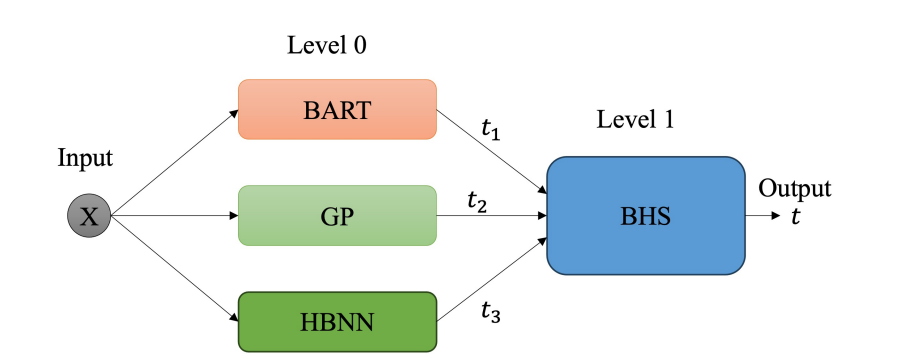
\includegraphics[width=0.65\linewidth]{stacking_arquitecture.png}
    \caption{Schematic architecture of the Bayesian Hierarchical Stacking model. The predictions from BART, GP and HBNN are combined through a first-level model that learns their relative weights.}
    \label{fig:bhsarch}
\end{figure}

\iffalse
ADD SOME BRIEF INTRO ABOUT BAYESIAN INFERENCE and statistics, PRIORS AND POSTERIORS, AND THE MODELS TO BE USED, WITHOUT NAMiNG THEM. NOT MORE Than ONE OR TWO PARAGRAPHS
Valuable source for this and other sections: Statistical Rethinking by Richard McElreath https://oceanrep.geomar.de/id/eprint/55819/1/Statistical%20Rethinking%202nd%20Edition.pdf. 
cafe example in page 413 is great to understand how a prior is learned from the data itself


W. K. Hastings, “Monte Carlo sampling methods usingMarkov chains and their applications,” Biometrika, vol. 57, no. 1, pp. 97–109, 04 1970 https://www2.stat.duke.edu/~scs/Courses/Stat376/Papers/Basic/Hastings1970.pdf


The objective of Markov Chain Monte Carlo (MCMC) methods is to construct a sequence of random samples (a Markov chain) where each state $S_i$ probabilistically depends exclusively on the preceding state $S_{i-1}$. Rather than executing a computationally intractable random grid search across all independent Gaussian distributions, the algorithm initiates at a random coordinate and proposes a sequential step (there's yt videos about this). If the proposed step moves toward a region of higher probability density within the posterior distribution, it is accepted. If it moves toward a less probable region, it is typically rejected, and the chain records the current position again. This mechanism allows the algorithm to efficiently map complex distributions with far fewer iterations than brute-force random sampling.

This sequential dependency introduces inherent drawbacks. Because $S_i$ is physically tethered to $S_{i-1}$, successive samples are highly autocorrelated and do not represent strictly independent draws from the posterior. To mitigate this, algorithms require an initial ``burn-in'' period (a large set of early iterations that are permanently discarded to allow the chain to reach the stationary distribution). Following burn-in, the chain must be thinned, storing only a subsampled fraction of the sequence (typically retaining only every $N$-th iteration) to approximate independent sampling. Despite these computational expenses, MCMC remains the optimal framework for sampling exact posterior distributions in highly parameterized deep learning models (R. Bardenet, A. Doucet, and C. Holmes, ``On Markov Chain Monte Carlo methods for tall data,'' J. Mach. Learn. Res., vol. 18, no. 1, pp. 1515–1557, Jan. 2017).

By tracking multiple independent Markov chains simultaneously, the algorithm thoroughly maps the hyperparameter space. This process inherently captures the learned covariance between variables, enforcing physical and mathematical limits on the parameter combinations that the respective probabilistic models evaluate.

\fi

\subsection{Bayesian Additive Regression Trees (BART)}
Among the three level-0 models used in this work, the practical deployment of the BART framework is mathematically and computationally the most straightforward, since its architecture requires relatively few tuning choices \citep{hill2020}. To understand the ensemble, the mechanics of a single regression tree must be defined. A tree recursively partitions the dataset by evaluating binary thresholds across input variables (e.g. $T_{\mathrm{eff}} < 5000\,\mathrm{K}$). At each step, the algorithm selects the threshold that maximizes the homogeneity of the target variable in the resulting subsets. When predicting for a new observation, the input traverses this learned path of decisions until it reaches a terminal node, or ``leaf''. The target variable prediction associated with that leaf is simply the mean value of the training points that occupy that specific terminal node.

% Explanation of "At each step, the algorithm selects the threshold that maximizes the homogeneity of the target variable in the resulting subsets.": Assume a parent node contains five stars with known masses: $[1.0, 1.1, 1.2, 5.0, 5.2]$.The algorithm tests possible splitting thresholds on an input variable (e.g., Effective Temperature).Split Option A: Creates Subset 1 $[1.0, 5.0]$ and Subset 2 $[1.1, 1.2, 5.2]$. Both subsets contain extreme high and low values. Internal variance is high. Homogeneity is low. The algorithm rejects this threshold.Split Option B: Creates Subset 1 $[1.0, 1.1, 1.2]$ and Subset 2 $[5.0, 5.2]$. The values inside Subset 1 are nearly identical to each other. The values inside Subset 2 are nearly identical to each other. Internal variance is minimized. Homogeneity is maximized. The algorithm selects this threshold.

The Bayesian Additive Regression Trees framework, introduced by \citet{chipman2010bart}, employs a sum-of-trees architecture to approximate complex non-linear functions. A Random Forest constructs an ensemble of deep, independent regression trees. By training each one of such trees on a random sample of the dataset and averaging the predictions of all of them, it produces a final output which reduces variance. BART follows this dataset subsampling logic, but the final predictions are not the average of the independent models, but the cumulative sum of the terminal node values across all interdependent trees in the ensemble. Therefore, in Random Forests every tree is a strong learner which produces an absolute value prediction for the target; while in BART the trees are weak learners, which just produce a part of the answer \citep{chipman2010bart}.

% Explanation of last part: in RF, you have 3 trees that give 1.9, 2.0 and 2.1. in BART, they giuve 1.5, 0.2 and 0.3.

This weak learner approach is mathematically guaranteed by regularisation priors, which constrain the size and structural influence of each tree. These mathematical penalties prevent any single tree component from dominating the overall model, thereby preserving the functional and computational advantages of the additive representation. Left unconstrained, the algorithm naturally drives individual trees to grow massive in pursuit of tighter data fits \citep{chipman2010bart}. The priors counteract this by forcing each tree to function as a weak learner, modelling only a restricted subset of the underlying function. This way, each tree provides only a small part of the predictor space, not a prediction itself.

Since each individual tree recursively partitions the predictor space utilising binary decision rules, the overall capacity and complexity of the model depends on the total number of trees. Predictive performance generally improves as this quantity increases, eventually reaching an asymptote.

Model optimisation follows the Bayesian backfitting MCMC scheme introduced in Section \ref{sec:bayesian-inference}. During each sweep, the algorithm updates one tree conditional on the partial residual left by the rest of the ensemble, proposing local changes such as growing, pruning or modifying a split. Repeating this process samples plausible tree structures and terminal-node values rather than selecting a fixed ensemble \citep{chipman2010bart}.

Crucially for stellar characterization, where uncertainty of the input features is a dominant factor, the framework used in this work accommodates an errors-in-variables approach. Inputs are not treated as static, exact measurements; rather, they are modeled as latent variables characterised by a Gaussian distribution whose variance is fixed by the observational uncertainties. This allows the model to account for the diverse uncertainties present across the entire star catalogue.



\subsection{Two-process Heteroscedastic Sparse Gaussian Process (GP)}
In classical parametric modelling, the functional form of the predictor is fixed in advance and inference is performed over its parameters. A Gaussian Process (GP) takes a different approach: it defines a probability distribution over possible functions. Any finite set of function values is assumed to follow a joint Gaussian distribution, so the model is specified by a mean function and a covariance function, or kernel. In many applications, the covariance function carries most of the information, while the mean function can be set to zero. Therefore, the main modelling choices are the prior covariance structure and the observational noise model, rather than an explicit fixed equation for the underlying function \citep{mackay1998gp,rasmussen2006gpml}.



% First, understand a multivariate gaussian: many variables, each in a gaussian distribution. A multivariate gaussian lives in a vector space, since each individual point has many components: point x has (x1, x2,...), point y has (y1, y2,...) and the gaussians followed are the gaussian conformed by (x1, y1...) the gaussian formed by (x2, y2...) and so on. If we extend these multivariate gaussian from a finite vector space to a continuous function space, we have a Gaussian Process (GP), where the elements are the functions (one element might be f(x, y) = sin x + y, the other might be g(x, y) = 2x + 6y). And the gaussian distributions are followed by the functions evaluated at the same points (f(2, 5) and g(2, 5); f(1, 0) and g(1,0)...). 

% The result of a gaussian distribution of vectors is a vector: the components of this result vector follow a gaussian, so for each iteration different numbers will be obtained, but overall they form a gaussian. The result of a gaussian distribution of functions is a function, where each point of the variable space follows a gaussian. But again, the result of an iteration is just a function with a fixed number for every coordinate in space. But these fixed numbers come from a gaussian dsitribution.


Training a GP therefore amounts to selecting a kernel and inferring its constraints, usually referred to as hyperparameters. The amplitude of the kernel controls the overall scale of the functions, and its length-scale controls how rapidly function values can change along the input axes. In this work, the kernel is chosen to favour smooth functions: nearby points in the input space are strongly correlated, while the correlation decreases as their separation increases. Large length-scales are thus dominant, since they produce slowly varying functions \citep{rasmussen2006gpml}.

% (additional info at the end of the text, to help you explain it better in the presentation)

% FINAL VERSION: MIGHT ERASE LAST SENTENCE OF THIS PARAGRAPH
To prevent the model from choosing unphysical hyperparameter values, priors are placed on the kernel length-scales and amplitudes. The version used in this work is the Automatic Relevance Determination (ARD) kernel, where each input dimension has its own length-scale, rather than sharing a single one. Dimensions with little predictive information can therefore be assigned very large length-scales, making them contribute less to the covariance structure \citep{rasmussen2006gpml}. The priors regularise this process by keeping the length-scales compatible with the spacing and span of the training data, while weakly informative amplitude priors avoid variances that collapse to zero or diverge.

The standard GP formulation usually assumes homoscedastic observational noise, meaning a single constant noise variance across the dataset. Stellar catalogues, however, contain measurements with uncertainties that vary between stars and between parameters. To account for this, the model used in this work follows a two-process heteroscedastic construction: one GP, $f(\boldsymbol{x})$, represents the latent predictive mean as a function of the stellar parameters, while a second GP, $g(\boldsymbol{\epsilon})$, models the logarithm of the noise variance from the reported measurement errors. This allows the predictive uncertainty to vary across the input space instead of being forced into a single global noise level \citep{le2005heteroscedasticgp}.

This flexibility comes with a computational cost. Because the kernel compares each data point with every other one, standard GP inference constructs an $N \times N$ covariance matrix; its diagonal terms describe each point's variance, while the off-diagonal terms encode similarity between different observations \citep{rasmussen2006gpml}. GP inference scales as $\mathcal{O}(N^3)$ because it requires operations on the full covariance matrix. To make inference feasible, both processes $f(\boldsymbol{x})$ and $g(\boldsymbol{\epsilon})$ are represented through a sparse approximation with $M$ inducing points, which act as representatives of the entire training set. Predictive covariances are therefore computed through the inducing set rather than directly through all pairwise relations between the $N$ observations, reducing the computational complexity to approximately $\mathcal{O}(NM^2)$ \citep{quinonero2005sparsegp}. Even so, Gaussian Processes can remain computationally demanding for large datasets.

The model is treated in a fully Bayesian way. As described in Section \ref{sec:bayesian-inference}, MCMC sampling explores plausible kernel hyperparameters, inducing variables and noise structures rather than fixing them at a single point with no uncertainty. Predictions are then averaged over these samples, propagating measurement and model uncertainty into the reported intervals.


% Additional info on the kernel function. First, picture the weight space. You have a set of data x, that we can fit to a linear regression model. But if we first apply a fixed function to these data, we can do the regression in the results (weight) space. We execute standard, computationally cheap linear matrix algebra in the 3D feature space, but the result projects back into the 1D input space as a non-linear parabola. Weight space allows linear algorithms to model non-linear geometries. We can extend the definition to function space: specifying a weight space and performing linear regression with a distribution of weights is mathematically identical to directly evaluating a kernel function between two points (evaluating the function itself, not fixed in this case).

% Additional way of understanding the length scale $\ell$: how far does one need to move (along a particular axis) in the input space for the function values to become uncorrelated.



\subsection{Hierarchical Bayesian Neural Network (HBNN)}
% "Traditional NN," "classical NN," and "point-estimate NN" all refer to the exact same thing: a standard neural network that uses fixed numbers for its weights, rather than probability distributions. ANN is just the broad category

% A bayesian neural network (BNN) is a stochastic artificial neural network (ANN) trained using Bayesian inference. So  just training an ANN with some probability distribution.


% other source: UNUSED: Weight Uncertainty in Neural Networks" by Blundell et al. (2015), USED a lot: Jospin et al. (2022) "Hands-on Bayesian Neural Networks - A Tutorial for Deep Learning Users"

% Good way of initially understanding neural newtorks:

% At its core, a neural network is an intricate sequence of mathematical operations. Data flows through hidden layers where every "neuron" calculates a sum by multiplying incoming data by adjustable **weights** and adding a baseline **bias**. To ensure the network can understand complex, real-world patterns rather than just plotting flat lines, this sum is passed through an activation function like **ReLU** (bc the other things are just linear). ReLU acts as a simple non-linear threshold (typically passing positive numbers through directly while turning any negative numbers into zero) which fundamentally allows the network to bend and shape its mathematical understanding of the data.

% The "learning" aspect is simply the automated, ongoing tuning of these equations to emulate reality. When a network first makes a prediction, its random weights produce an incorrect answer. By comparing its mathematical output to the true, real-world answer, the system calculates the exact error and uses a process called **backpropagation** to work backward through the layers, systematically tweaking every single weight and bias. After thousands or millions of these microscopic adjustments, the network's internal math becomes perfectly balanced to reliably transform new inputs into highly accurate predictions.

At its core, an artificial neural network is a sequence of mathematical operations arranged in layers. Neural networks are used to approximate non-linear relations by applying successive linear transformations and non-linear activation functions to the input data. In a standard network, the weights and biases in each layer are fitted as fixed point estimates. This can provide accurate predictions, but it does not naturally represent uncertainty in the model parameters and may produce overconfident results outside the region well covered by the training data \citep{jospin2022bnn}. 

Bayesian Neural Networks (BNNs) address this limitation by assigning probability distributions to the weights and biases instead of single values. After conditioning on the data, the prediction is obtained by averaging over an ensemble of possible networks, making model uncertainty part of the prediction itself \citep{blundell2015weight}. In the hierarchical formulation used in this work, the model also accounts for the finite precision of the observations, not only for uncertainty in the neural-network weights and biases \citep{jospin2022bnn}. This distinction is central for stellar characterization, where sparse training regions and measurement errors both affect the reliability of the final prediction.


\begin{figure}[H]
\centering

\begin{subfigure}[t]{0.36\textwidth}
    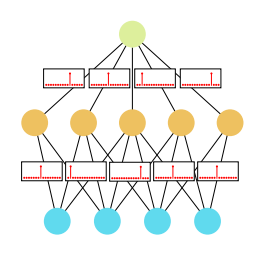
\includegraphics[width=\textwidth]{understandBNN_panel_a_point_estimate.png}
    \caption{Point-estimate NN.}
    \label{fig:nn_point_estimate}
\end{subfigure}\hspace{1.5cm}
\begin{subfigure}[t]{0.36\textwidth}
    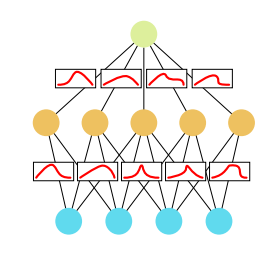
\includegraphics[width=\textwidth]{understandBNN_panel_b_weight_distributions.png}
    \caption{BNN with weight distributions.}
    \label{fig:bnn_weight_distributions}
\end{subfigure}

\caption{Comparison between neural-network formulations. Figure \ref{fig:nn_point_estimate} shows a standard network, in which the weights and biases are fixed after training. Figure \ref{fig:bnn_weight_distributions} shows the Bayesian formulation used in this work, where probability distributions are assigned to the weights and biases. Adapted from \citep{jospin2022bnn}.}
\label{fig:noseno}
\end{figure}

The network itself uses Gaussian priors for the weights and biases and a two-layer architecture with Leaky ReLU activations \citep{maas2013rectifier}. As discussed in Section \ref{sec:bayesian-inference}, MCMC sampling explores the posterior distribution rather than converging to a single point with no uncertainty. The HBNN therefore keeps the flexibility of neural networks while preserving the probabilistic interpretation required for calibrated stellar predictions \citep{jospin2022bnn}.





% for the presentation, also keep in mind that andy always describes these neural neetworks as a sort of one layer, many branches to many layers, many levels of layers, and then they converge to one putput (see fig 1 of 2022). the key is the boceto, to illustrate it. might look for somehting similar, either for resentation itself or for blackboard explanation when in questions



\iffalse

This approach improves results because aggregating predictions from a large ensemble of distinct, independent models generally yields superior predictive accuracy compared to relying on a single deterministic model (galton1907voxpopuli and breiman1996bagging). However, the primary motivation for employing BNNs isn't their enhanced prediction ability, but their rigorous quantification of uncertainty. By evaluating the variance across the multiple sampled models, BNNs provide a mathematically sound measure of prediction confidence, significantly reducing overconfidence compared to classical ANNs (J. Mitros and B. M. Namee, ``On the validity of Bayesian neural networks for uncertainty estimation,'' in AICS, 2019; AND ALSO A. Kristiadi, M. Hein, and P. Hennig, ``Being Bayesian, even just a bit, fixes overconfidence in ReLU networks,'' CoRR, vol. abs/2002.10118, 2020. [Online]. Available: http://arxiv.org/abs/2002.10118). Furthermore, BNNs distinguish between epistemic uncertainty (model uncertainty due to a lack of data) and aleatoric uncertainty (inherent noise within the data itself) (A. D. Kiureghian and O. Ditlevsen, ``Aleatory or epistemic? does it matter?'' Structural Safety, vol. 31, no. 2, pp. 105–112, 2009). This distinction makes BNNs highly data-efficient and less susceptible to overfitting on small datasets (S. Depeweg, J.-M. Hernandez-Lobato, F. Doshi-Velez, and S. Udluft, ``Decomposition of uncertainty in Bayesian deep learning for efficient and risk-sensitive learning,'' in Proceedings of the 35th International Conference on Machine Learning, vol. 80, 2018, pp. 1184–1193).


In this work, we deploy a Hierarchical Bayesian Neural Network (HBNN). A hierarchical (or multilevel) model separates inference into distinct, interconnected levels. In a standard hierarchical structure, the parameters defining a base-level probability distribution are not fixed scalars; rather, they are themselves governed by higher-level probability distributions, known as hyperpriors. In our specific HBNN, the hierarchy distinctly separates the physical modeling of the stellar input parameters from the non-linear regression performed by the network.


Standard errors-in-variables models treat input predictors as independent. Level 1 of the HBNN explicitly models the physical correlations between the measured inputs (e.g., the relationship between effective temperature and surface gravity). So is this just the parameters of the layers and hidden layers?

The true, unobservable physical parameters are treated as latent variables, denoted $x_{\mathrm{latent}}$. To model their interdependencies, $x_{\mathrm{latent}}$ is assigned a zero-mean multivariate normal prior:
\begin{equation}
    x_{\mathrm{latent}} \sim \mathcal{N}(0, \Sigma)
\end{equation}
where $\Sigma$ is the covariance matrix. We utilize an LKJ Cholesky prior (Lewandowski et al., 2009) for the correlation matrix components of $\Sigma$, a standard formulation ensuring the matrix remains mathematically valid. This level links the reported instrumental measurements and their $1\sigma$ errors to the latent variables, calculating a joint probability distribution that accounts for both measurement noise and intrinsic physical correlations. Gaussian distributions are predominantly utilized here and throughout the model due to their computational tractability and ease of generalization to higher dimensions.

In Level 2, the joint probability distribution of $x_{\mathrm{latent}}$ calculated in Level 1 serves as the input to the stochastic neural network, mapping the correlated stellar parameters to the target variable (e.g. stellar mass, $M$). 

Because the network is Bayesian, independent Gaussian priors are placed on all network weights and biases. The architecture utilizes a two-layer structure with a Leaky ReLU activation function, which prevents training from ending too early (bc the gradient vanishes during training). (Maas, A. L., Hannun, A. Y., and Ng, A. Y. (2013). Rectifier nonlinearities improve neural network acoustic models. In Proc. icml (Vol. 30, No. 1, p. 3)). 
Training is executed via Markov Chain Monte Carlo (MCMC) sampling. Rather than utilizing standard gradient descent to converge on a single optimal configuration, MCMC algorithms traverse the high-dimensional parameter space to iteratively sample from the posterior distribution, mathematically generating the required ensemble of stochastic models.

\fi

% Explanation: In deep networks, standard activation functions (like Sigmoid or regular ReLU) can cause the gradients (the math used to update the weights during training) to become $0$. If the gradient is $0$, the network stops learning

% Likelihood is the mathematical probability of observing your exact training data given a specific set of model parameters. It quantifies how accurately a proposed model configuration reproduces the measured target variables.


\subsection{Bayesian Hierarchical Stacking}
The predictions from BART, GP and HBNN are combined through Bayesian Hierarchical Stacking (BHS). Stacking is an ensemble method in which the outputs from several models are combined using learned weights, allowing relevant information from each model to contribute to the final prediction \citep{wolpert1992stacked}. Unlike simple averaging, BHS allows the weights assigned to each level-0 predictor to depend on the input features. This is important because a model may be reliable for near-solar stars but less reliable for more massive objects or for stars with larger uncertainties. The former is the case of the level-0 models used in this work, as described in Section \ref{sec:results}. The final estimate is therefore a locally weighted combination of the three model outputs \citep{yao2022hierarchicalstacking}.

The weights are estimated using cross-validation information, discussed in Section \ref{sec:evaluation}. The hierarchical formulation regularizes the variation in these weights, preventing the stacking model from reacting too strongly to noise in sparsely populated regions of the dataset. Thus, BHS is used as a controlled way to exploit the complementary strengths of the three models while reducing the risk of relying on a single imperfect predictor.


\iffalse

In this context, an individual predictive algorithm or model is referred to as a \textit{generalizer}. By partitioning the training set, training generalizers on one partition, and evaluating them on the other, we can deduce and mathematically correct for the individual biases of each generalizer. Loosely speaking, this strategy combines the generalizers rather than choosing amongst them. This is achieved by taking the output predictions of the base models as input components in a new mathematical space, and then deploying a meta-model to generalize within that new space (David Wolpert. Stacked generalization. Neural Networks, 5:241–259, 12 1992. doi: 10.1016/S0893-6080(05)80023-1).

In our framework, the base generalizers (level-0 models) correspond to our $K=3$ independently fitted probabilistic predictors, each providing a posterior predictive distribution $p_k(y \mid \mathbf{x})$. Our level-0 models are the Bayesian Additive Regression Trees (BART), Gaussian Process (GP), and hierarchical Bayesian neural network (HBNN) discussed previously. A level-1 meta-model is then used to learn how to optimally combine these predictions.


Standard model averaging assigns a fixed, global weight to each model based on overall performance. However, in hierarchical stacking, the weights are not fixed per model; they vary dynamically with the input data. This is crucial because different models can be highly effective at explaining different physical regions of the input space cite yao 2022. Therefore, BHS can be conceptualized as point-wise model averaging.

The stacking weights are estimated by maximizing the leave-one-out (LOO) expected log predictive density, which we approximate using Pareto-smoothed importance sampling (PSIS-LOO) [cite vehtari 2017}]. see Section \ref{sec:evaluation} 

To achieve spatially varying weights across the predictor space, the framework introduces latent, unconstrained variables (logits) (add reference).


Permitting weights to vary freely across the input space risks severe overfitting. To regularize the feature dependence of the weights, we apply a hierarchical prior to the regression coefficients $\beta_k$. Each coefficient vector is modeled as a Gaussian:
\begin{equation}
\beta_{kj} \sim \mathcal{N}(\mu_k, \sigma_k^2), \qquad j = 1, \dots, d,
\label{eq:beta_prior}
\end{equation}
where $d$ is the number of input variables. This hierarchical construction mathematically links the coefficient distributions across the different models. It effectively shrinks $\beta_k$ toward a model-specific mean unless the empirical data provides strong evidence for feature dependence. This balances local adaptation with global regularization.

The use of this two-level architecture is sufficient and robust because the level-1 model does not artificially invent new predictive structures for the target variable; it strictly learns the optimal spatial combination of the probabilistic level-0 predictors. Crucially, uncertainty is rigorously propagated throughout the entire procedure. The epistemic and aleatoric uncertainties inherent to the stellar parameters are captured within the level-0 posteriors $p_k(y \mid \mathbf{x})$, while the uncertainty regarding which model to trust is captured within the posterior of the stacking weights $(\beta_k, \mu_k, \sigma_k)$. In this work, unless stated otherwise, we report final predictions using the posterior mean of $w_k(\mathbf{x}_*)$ evaluated at a new input $\mathbf{x}_*$.

\fi

\subsection{Model Evaluation through Cross-validation} \label{sec:evaluation}
% Data extracted from Rasmussen and Williams (2006).

Model evaluation estimates how well a trained model will generalize to stars that were not used during training. A simple train--validation split gives a direct test of this: part of the dataset is kept aside as a validation subset, and the trained model is then evaluated against it. Nevertheless, the result can depend strongly on the particular partition, since a large validation set reduces the data available for fitting, while a small one gives a noisy estimate of the error \citep{rasmussen2006gpml}.

Cross-validation reduces this dependence on a single split. In $k$-fold cross-validation, the dataset is divided into $k$ subsets; each subset is used once for validation while the remaining subsets are used for training. The reported performance is then averaged over the folds, so every star contributes both to fitting and to out-of-sample assessment \citep{rasmussen2006gpml}. This provides a more stable basis for evaluating the target-variable predictions produced by the models used in this work, allowing for a better comparison between them.

The most exhaustive version is Leave-One-Out Cross-Validation (LOO-CV), where each observation is validated once while the model is trained on all remaining observations. For complex Bayesian models, explicitly refitting the model for every observation is usually too expensive. Therefore, when appropriate, this work uses the efficient LOO approximation proposed by \citet{vehtari2017loo}: Pareto-smoothed importance sampling (PSIS-LOO). This gives a common evaluation criterion without requiring a separate validation set.

\iffalse

To evaluate predictive performance, datasets are traditionally partitioned into distinct training and validation subsets. The model optimizes its parameters on the training set, while the validation set provides an empirical measure of the generalization error, defined as the expected prediction error on unseen, independent data points. 

However, a static train-validation split presents inherent mathematical limitations. Withholding a large fraction of data for validation starves the model of valuable training information, whereas employing a small validation set results in high-variance, unreliable performance estimates (Rasmussen and Williams, 2006). 

To mitigate these drawbacks, $k$-fold cross-validation is employed. This technique partitions the dataset into $k$ disjoint (mutually exclusive) subsets of equal size. In a single iteration, one subset acts as the validation hold-out, while the remaining $k-1$ subsets are aggregated to train the model. This protocol is iterated $k$ times until every subset has served exactly once as the validation set. Consequently, a vast majority of the data is utilized for training in each fold, and every observation is ultimately evaluated as an unseen validation case.

Despite its statistical advantages, standard $k$-fold cross-validation imposes severe computational burdens, as the model must be completely refitted $k$ times. The logical extreme of this method occurs when $k = n$, where $n$ is the total number of observations. This is known as Leave-One-Out Cross-Validation (LOO-CV). While theoretically optimal for performance estimation, standard LOO-CV is computationally intractable for complex Bayesian models, necessitating advanced mathematical approximations (such as Pareto-smoothed importance sampling (PSIS-LOO)) to evaluate the predictive density without requiring explicit refitting (Rasmussen and Williams, 2006).

\fi

\section{Methods} \label{methods}
% A medida que expliques como cada uno de los metodos utiliza las observaicioens directas para calcular parametros, puedes mencionar los papers qu ehayas ido usando. Esto hazlo en el futuro, cuando releas los papers para hacer unos parrafos de explicacion de cada uno de ellos

This section introduces the observational basis of the stellar labels used later to construct the final catalogue. The catalogue is built from three reference methods: detached eclipsing binaries, asteroseismology and interferometry. Spectroscopy is discussed first as context, because it is essential for many stellar parameters, but relies strongly on stellar-atmosphere modelling. This contrast motivates the use of the other three methods as the main sources of high-quality labels, while also making clear that they are not completely free from auxiliary assumptions.

\subsection{Spectroscopy}
%revisar si esta(s) seccion(es) tiene un tono demasiado didactico, lejos de un paper/TFG

%  spectroscopy study the distribution of electromagnetic radiation as a function of wavelength. photometry studies this distribution in large intervals, selected by means of filters, while spectroscopy makes a finer analysis, with higher resolution, by means of optical dispersion devices, such as optical prisms and diffraction gratings. So spectroscopy = wavelength separation
Spectroscopy analyses the stellar radiation received as a function of wavelength. The continuum, discontinuities, absorption lines and molecular bands are produced by physical processes in the stellar atmosphere, and therefore contain information about stellar parameters.

The difficulty is that these quantities are not usually obtained by direct measurement. They are inferred by comparing the observed spectrum with synthetic spectra, line lists and stellar-atmosphere models \citep{tsantaki2018}. Spectroscopy is therefore essential, especially for $T_{\mathrm{eff}}$ and $[\mathrm{Fe}/\mathrm{H}]$, but it can also introduce model-dependent assumptions into any machine-learning model trained on those input features.

%maybe add something about photometry . say that it is very similar or smth. it prolly need atmospheric methods as well. also mention astrometry, which I think doesn't rely on atmopshere, but needs very precise and hard to obtain data, and take too much time to measure. exoplanet transits happen very rarely


\subsection{Eclipsing Binaries}
%add this somewhere, if I find a refernce: DEBs are considered the absolute pinnacle for determining stellar mass and radius.
Detached eclipsing binaries are systems in which two stars orbit each other without significant mass transfer, while their orbital plane causes periodic eclipses as seen from Earth. Because the components are dynamically linked but remain physically separated, they are especially valuable for obtaining fundamental stellar parameters such as $M$ \citep{Southworth2015,Eker2018}.

The measured light curve gives the orbital period, eclipse geometry, relative radii and temperature ratio. Radial-velocity measurements from Doppler shifts then provide the orbital velocities. Combining these observables with Keplerian dynamics yields absolute masses and radii, from which density and surface gravity follow. These quantities are therefore mainly geometric and dynamical.

The atmospheric quantities are less direct. Absolute temperatures and luminosities usually require spectroscopy, colour-temperature relations, parallax, bolometric fluxes, or a combination of these ingredients \citep{Graczyk2022}. For this reason, detached eclipsing binaries are treated as a strong reference source for masses and radii, while their temperature and luminosity labels still require attention to the assumptions used to derive them.

% Revisar que estos dos metodos se cumplan luego en los papers. Puede haber menos, o mas.

\subsection{Asteroseismology}
%revisar si esta(s) seccion(es) tiene un tono demasiado didactico, lejos de un paper/TFG. sobre todo el final sobre los harmonicos

% Rodrigues 2017 explains well this method (especially the used parameters delta nu and nu_max) in its introduction
Asteroseismology studies stellar oscillations. An extensively studied type of oscillations occurs in solar-like stars, where turbulent motion in the outer convective envelope excites pressure waves that propagate through the interior and produce small brightness variations. Time-series photometry and Fourier analysis reveal the characteristic oscillation frequencies of the star \citep{Bellinger2019,Serenelli2021}.

Two global seismic quantities are especially useful. The large frequency separation, $\Delta\nu$, scales with the square root of the mean density, while the frequency of maximum oscillation power, $\nu_{\mathrm{max}}$, is related to surface gravity and effective temperature:
\begin{equation}
\Delta\nu \propto \sqrt{\frac{M}{R^3}}, \qquad
\nu_{\mathrm{max}} \propto \frac{M}{R^2\sqrt{T_{\mathrm{eff}}}} .
\end{equation}
With an external estimate of $T_{\mathrm{eff}}$, these relations constrain mass, radius and $\log g$ \citep{chaplin2013}.

This makes asteroseismology particularly useful for single stars, where direct dynamical masses are usually unavailable. However, the method still depends on scaling relations, external atmospheric inputs and, in more detailed analyses, stellar models. It therefore provides strong constraints, but not completely model-independent labels.

% Asteroseismic $\log g$ values are far more precise than any other method for single stars. (add reference

\subsection{Interferometry}
Interferometry combines the light collected by separated telescopes, effectively increasing the angular resolution beyond that of a single aperture. For nearby bright stars, this makes it possible to measure the angular diameter. Together with an independent distance, usually from parallax, the stellar radius can then be obtained geometrically \citep{ligi2016}.

If the bolometric flux is also known, the effective temperature follows from the Stefan--Boltzmann relation. This makes interferometry one of the most empirical routes to stellar radii and temperatures, and it is used in benchmark-star calibrations \citep{Soubiran2024}. The method is not fully assumption-free, because bolometric flux estimates require extinction corrections and model-dependent treatment of unobserved spectral regions. It is also limited to stars with sufficiently large angular diameters, so its contribution to the total sample is small.

\subsection{Limits of Model Independence}
MIGHT REMOVE THIS SECTION. NOT BECAUSE OF SPACE; BUT AVOIDING UNNCESSARY REPETITION

The methods described above are used because they reduce the dependence on stellar-atmosphere models, but they do not remove modelling assumptions completely. Eclipsing binaries still require external calibrations for absolute temperatures and luminosities, asteroseismic masses and radii depend on scaling relations and an external $T_{\mathrm{eff}}$ estimate, and interferometric temperatures require bolometric fluxes and extinction corrections.

For this reason, the catalogues used in this work should not be interpreted as perfectly model-independent ground truth. They are instead high-quality reference labels, selected because their central constraints are closer to geometry or dynamics than to atmospheric modelling: eclipsing binaries provide strong masses and radii, asteroseismology constrains stellar density and surface gravity, and interferometry gives empirical radii and temperatures for suitable nearby stars. This compromise is important for the machine-learning models trained later, since their predictions cannot be more physically reliable than the labels from which they learn.


\section{Data} \label{sec:data}
% This paper talks about prioritising Data instead of models. Not prioritising good data over a large quantity of data. It explicitly says it wants high quality and quantity of data. Might use it in the future, tho. https://www.semanticscholar.org/paper/Data-centric-Artificial-Intelligence%3A-A-Survey-Zha-Bhat/12c6be503e4e5b7c9cb1810152d4364f26628a8d Zha et al., 2023

In supervised machine learning, the quality of the input features can be as important as the size of the training set. Large catalogues affected by heterogeneous systematics may lead the models to reproduce those biases instead of learning the underlying physical relations \citep{li2021dataquality}. For this reason, this work follows a quality-centred strategy, prioritising a smaller, traceable and physically reliable calibration set over a larger but less controlled sample.

Following the guidance of \citet{moya2018}, whose catalogue covered approximately the mass range $0.7\,M_\odot < M < 2.5\,M_\odot$, an extended stellar catalogue was assembled from literature sources with complementary parameter coverage. The lower boundary has been reduced to $0.5\,M_\odot$, since one of the aims of this extension was to improve the coverage at lower masses. Such reference stars are needed to calibrate predictions for M-type stars, which are especially relevant in exoplanet studies (see Section \ref{subsec:dataset_b}). The aim was to obtain a statistically meaningful and heterogeneous sample, while preserving clear information on the uncertainties of the stellar parameters. Because the reported uncertainties are propagated into the final mass predictions in the probabilistic models in this work, this uncertainty-treatment is a key aspect.

As explained in Section \ref{methods}, the reference sources were selected according to three observational methods: eclipsing binaries, asteroseismology and interferometry. Studies published between 2018 and 2025 were reviewed when they provided uncertainties and as many of the required stellar parameters as possible, listed in Table \ref{MS_catalog_database_D}. Stellar mass and radius were mandatory, since stellar densities were computed from them. This initial compilation contained 16094 stars before duplicate removal and quality cleaning.

\begin{table}[H]
\centering
\setlength{\tabcolsep}{4pt}
\caption{Summary of the stellar parameters contributed by each catalogue to the final calibration sample of 767 usable main-sequence stars. Each value gives the number of stars with the corresponding available parameter. The metallicity column combines $[\mathrm{Fe}/\mathrm{H}]$ and $[\mathrm{M}/\mathrm{H}]$. Catalogues not individually discussed in this work are described in \citet{moya2018}.}
\footnotesize
\begin{tabular}{lrrrrrrrr}
\hline\hline
Catalogue & $M$ & $R$ & $T_{\mathrm{eff}}$ & $L$ & Meta & $\log g$ & $\rho$ & $a$\\
~ & ($M_\odot$) & ($R_\odot$) & (K) & ($L_\odot$) & (dex) & (dex) & ($\rho_\odot$) & ($R_\odot$)\\
\hline
Serenelli et al. (2017) & 240 & 240 & 240 & 240 & 240 & 240 & 240 & 0\\
Xiong et al. (2023) & 141 & 141 & 141 & 141 & 141 & 141 & 141 & 141\\
Chaplin et al. (2014, SDSS) & 62 & 62 & 62 & 62 & 62 & 62 & 62 & 0\\
Eker et al. (2014) & 54 & 54 & 54 & 54 & 54 & 54 & 54 & 54\\
Yildiz et al. (2019) & 42 & 42 & 42 & 42 & 42 & 42 & 42 & 0\\
Lund et al. (2016) & 28 & 28 & 28 & 28 & 28 & 28 & 28 & 0\\
Huber et al. (2013) & 24 & 24 & 24 & 24 & 24 & 0 & 24 & 0\\
Silva Aguirre et al. (2015) & 24 & 24 & 24 & 24 & 24 & 24 & 24 & 0\\
Wang et al. (2025) & 20 & 20 & 20 & 20 & 20 & 20 & 20 & 20\\
Eker et al. (2014, 2018) & 17 & 17 & 17 & 17 & 17 & 17 & 17 & 17\\
Silva Aguirre et al. (2017) & 15 & 15 & 15 & 15 & 15 & 15 & 15 & 0\\
Soubiran et al. (2024) & 13 & 13 & 13 & 13 & 13 & 13 & 13 & 0\\
Helminiak et al. (2019) & 11 & 11 & 11 & 11 & 11 & 11 & 11 & 11\\
Pan et al. (2025) & 10 & 10 & 10 & 10 & 10 & 10 & 10 & 10\\
Ligi et al. (2016) & 10 & 10 & 10 & 10 & 10 & 0 & 10 & 0\\
Chaplin et al. (2014, Bruntt) & 8 & 8 & 8 & 8 & 8 & 8 & 8 & 0\\
Özdarcan et al. (2025, Feb.) & 7 & 7 & 7 & 7 & 7 & 7 & 7 & 7\\
Malkov et al. (2007) & 4 & 4 & 4 & 4 & 4 & 0 & 4 & 0\\
Welsh et al. (2012) & 4 & 4 & 4 & 4 & 4 & 4 & 4 & 4\\
Brogaard et al. (2018) & 3 & 3 & 3 & 3 & 3 & 3 & 3 & 3\\
Özdarcan et al. (2024) & 3 & 3 & 3 & 3 & 3 & 3 & 3 & 3\\
Torres et al. (2010) & 3 & 3 & 3 & 3 & 3 & 3 & 3 & 3\\
Çakırlı et al. (2025, Apr.) & 2 & 2 & 2 & 2 & 2 & 2 & 2 & 2\\
Çakırlı et al. (2025, Dec.) & 2 & 2 & 2 & 2 & 2 & 2 & 2 & 2\\
Knudstrup et al. (2020) & 2 & 2 & 2 & 2 & 2 & 2 & 2 & 2\\
Martin et al. (2024, Dec.) & 2 & 2 & 2 & 2 & 2 & 2 & 2 & 2\\
Miller et al. (2022) & 2 & 2 & 2 & 2 & 2 & 2 & 2 & 2\\
Miller et al. (2026) & 2 & 2 & 2 & 2 & 2 & 2 & 2 & 2\\
O'Brien et al. (2025) & 2 & 2 & 2 & 2 & 2 & 2 & 2 & 2\\
Xu et al. (2026) & 2 & 2 & 2 & 2 & 2 & 2 & 2 & 2\\
Yücel et al. (2026) & 2 & 2 & 2 & 2 & 2 & 2 & 2 & 2\\
Bond et al. (2020) & 1 & 1 & 1 & 1 & 1 & 1 & 1 & 1\\
Jennings et al. (2024) & 1 & 1 & 1 & 1 & 1 & 1 & 1 & 0\\
Lund et al. (2019) & 1 & 1 & 1 & 1 & 1 & 1 & 1 & 0\\
Maxted et al. (2023) & 1 & 1 & 1 & 1 & 1 & 1 & 1 & 1\\
Maxted et al. (2025) & 1 & 1 & 1 & 1 & 1 & 1 & 1 & 1\\
Thomsen et al. (2022) & 1 & 1 & 1 & 1 & 1 & 1 & 1 & 1\\
Total & 767 & 767 & 767 & 767 & 767 & 729 & 767 & 295\\
\hline
\end{tabular}
\label{MS_catalog_database_D}
\end{table}

\subsection{Catalogues}
The literature sources used to compile the catalogue are summarised in Table \ref{tab:catalogue_sources}. The main role of each source in the construction of the final sample, is also indicated, since not all catalogues contributed the same type of information.

\begin{table}[H]
\centering
\caption{Summary of the main literature sources used to build the stellar catalogue. The initial-entries column gives the number of main-sequence stars taken from each source before duplicate removal and further quality cleaning (see Section \ref{sec:cleaning}). The method column indicates the main observational basis of each source, while the final column summarises its role in the catalogue construction and any relevant technical treatment applied during the merging process.}
\label{tab:catalogue_sources}
\scriptsize
\setlength{\tabcolsep}{3pt}
\renewcommand{\arraystretch}{1.12}
\begin{tabular}{p{0.17\linewidth}p{0.09\linewidth}p{0.18\linewidth}p{0.22\linewidth}p{0.27\linewidth}}
\hline\hline
Source & Initial entries & Main method & Main contribution & Notes for this work \\
\hline
\citet{Eker2018} & 508 & Detached eclipsing binaries & Accurate stellar parameters for main-sequence binary components over a broad mass range & Used as a high-quality reference for masses and radii; also relevant for calibrating $L$ and $T_{\mathrm{eff}}$. \\
\hline
\citet{Helminiak2019} & 22 & Detached eclipsing binaries with spectroscopic support & Binary-star parameters with additional atmospheric information & Treated with care because the reported abundance information was given as $[\alpha/\mathrm{Fe}]$, not directly in the metallicity scale adopted here. \\
\hline
\citet{Graczyk2021,Graczyk2022} & 28 & Detached eclipsing binaries & Surface-brightness--colour calibration samples & The dwarf-star calibrating sample of \citet{Graczyk2022} was adopted as a strong reference source. \\
\hline
\citet{Nsamba2025} & 8 & Benchmark stars & Pre-existing benchmark-star compilation & Required careful duplicate removal because of overlap with other catalogues. \\
\hline
\citet{Bellinger2019} & 97 & Asteroseismology & Asteroseismic masses and radii for mostly solar-like stars & Several objects lacked some atmospheric parameters required in this work. \\
\hline
\citet{Serenelli2021} & 106 & Mixed benchmark compilation & Stellar mass-determination methods across the HR diagram, including eclipsing binaries and asteroseismology & Contributed a large number of reliable stars, although luminosity and metallicity were not always available. \\
\hline
\citet{Soubiran2024} & 31 & Interferometry and benchmark-star calibration & Gaia FGK benchmark stars with fundamental $T_{\mathrm{eff}}$ and $\log g$ & Luminosities were provided as $\log L$, requiring conversion before use in the catalogue. \\
\hline
\citet{Xiong2023} & 354 & Eclipsing binaries with spectroscopic information & Empirical library based on binary-star parameters & Treated with additional caution because of non-standard identifiers and some comparatively large uncertainties. \\
\hline
\citet{Sayeed2025} & 694 & Asteroseismology & Homogeneous catalogue of Kepler main-sequence and subgiant solar-like oscillators & Metallicity was not always accompanied by uncertainty. \\
\hline
\citet{Yildiz2019} & 74 & Asteroseismology & Masses and radii for Kepler and CoRoT solar-like oscillators & Metallicities reported as surface metal mass fractions were converted to the logarithmic scale. \\
\hline
\end{tabular}
\end{table}


\citet{Yildiz2019} provided metallicities as surface metal mass fractions $Z_s$. They were converted to the logarithmic scale using $[\mathrm{M}/\mathrm{H}] = \log \left[(Z_s/X_s)/(Z/X)_\odot\right]$, adopting $X_s \simeq 0.7381$ and $(Z/X)_\odot = 0.0181$ from \citet{asplund2009}.


% \citet{Southworth2015} is the famous DEBCat, but it didn't finally make the sample because L was computed from model-dependet methods

\subsection{Cleaning} \label{sec:cleaning}
When the same star appeared in several catalogues, the retained entry was chosen according to the reliability of the source. Priority was given to catalogues providing the most direct stellar parameters, smaller reported uncertainties and a more complete set of parameters. Regularly updated catalogues and benchmark-star compilations were also preferred over more heterogeneous or less traceable sources. This meant favouring high-precision eclipsing-binary catalogues such as \citet{Eker2018} and the calibrating samples of \citet{Graczyk2022}, benchmark compilations such as the Gaia FGK benchmark-star catalogue \citep{Soubiran2024}, and samples cross-validated across different methods, such as those in \citet{Serenelli2021}. After duplicate removal, 13783 stars remained.

The cleaned sample was then restricted to main-sequence candidates using a criterion based on $\log g$. Following \citet{bilir2008}, stars with $\log g > 4.0$ were classified as main-sequence objects, except for extremely large values of $\log g$ ($\gtrsim 5.5$), which were not interpreted as normal main-sequence stars. Although this threshold is approximate, the effect of applying different classification criteria was already analysed by \citet{moya2018}. They found that the choice between a simple threshold and a more robust classification method had little influence on the final results. The $\log g$ criterion adopted here was therefore considered sufficient for the purposes of this work.

1915 stars remained after this selection, although not all of them contained every required parameter. In principle, incomplete entries could be retained in a Bayesian framework by treating missing quantities as latent variables, provided that an explicit model for the missing-data process is specified \citep[p.~511]{mcelreath2020}. In this work, however, parameter completeness and direct traceability were prioritised, so this kind of imputation was not used. % IDK what latent means here

% \begin{table}[H]
% \centering
% \caption{Secondary sources used to complement missing stellar parameters. During the catalogue merging process, when a preferred primary source (Output catalogue) lacked data for specific parameters, the gaps were filled using the secondary catalogues listed in the corresponding columns.}
% \begin{tabular}{c}
% Ejemplo tabla que tarda poco en compilar\\
% \end{tabular}
% \label{Tab:secondary sources}
% \end{table}

The newly compiled 1915-star sample was then cross-matched with the catalogue of \citet{moya2018} in order to merge both sources, while avoiding duplicates and retaining only the highest-quality entries. Following the same data-centred strategy, stars were removed when they had excessively large uncertainties, zero reported uncertainty in any parameter except $a$, were not classified as main-sequence stars in both catalogues, or had duplicated identifiers. This reduced the sample to 784 stars. Section \ref{subsec:dataset_a} explains the later removal of 17 additional objects, leading to the final training sample of $n=767$ stars.

Although each star in the final merged sample is assigned a primary catalogue identifier according to the reliability criteria described above, the individual stellar parameters for a given entry do not always originate from that single source. To maximise completeness, the merging algorithm constructed composite entries: when the primary catalogue lacked a given parameter, the missing value was filled from an available secondary catalogue. The final parameter set for a star can therefore be heterogeneous in origin. To preserve traceability, a more detailed internal provenance table was used alongside Table \ref{MS_catalog_database_D}; for each primary source, it records which secondary catalogues were queried to fill each missing parameter. When several secondary sources were available, they were prioritised according to the reliability hierarchy described above.

The Hertzsprung--Russell diagram was used as a final consistency check for the cleaned sample. This diagram relates stellar luminosity to effective temperature and is commonly used to identify evolutionary stages, especially the main sequence. As shown in Figure \ref{fig:HRdiagram}, the stars mostly follow the expected main-sequence behaviour, with luminosity decreasing towards lower effective temperatures. FGK stars occupy approximately $T_{\mathrm{eff}} \sim 3500$--$7400\,\mathrm{K}$ \citep{pecaut2013}, or $\log_{10}T_{\mathrm{eff}} \sim 3.54$--$3.87$. Most of the sample lies in this regime, especially the asteroseismic and interferometric stars. The eclipsing-binary subsample is also mainly concentrated around the main sequence, but it spans a broader region of the diagram.

\begin{figure}[H]
    \centering
    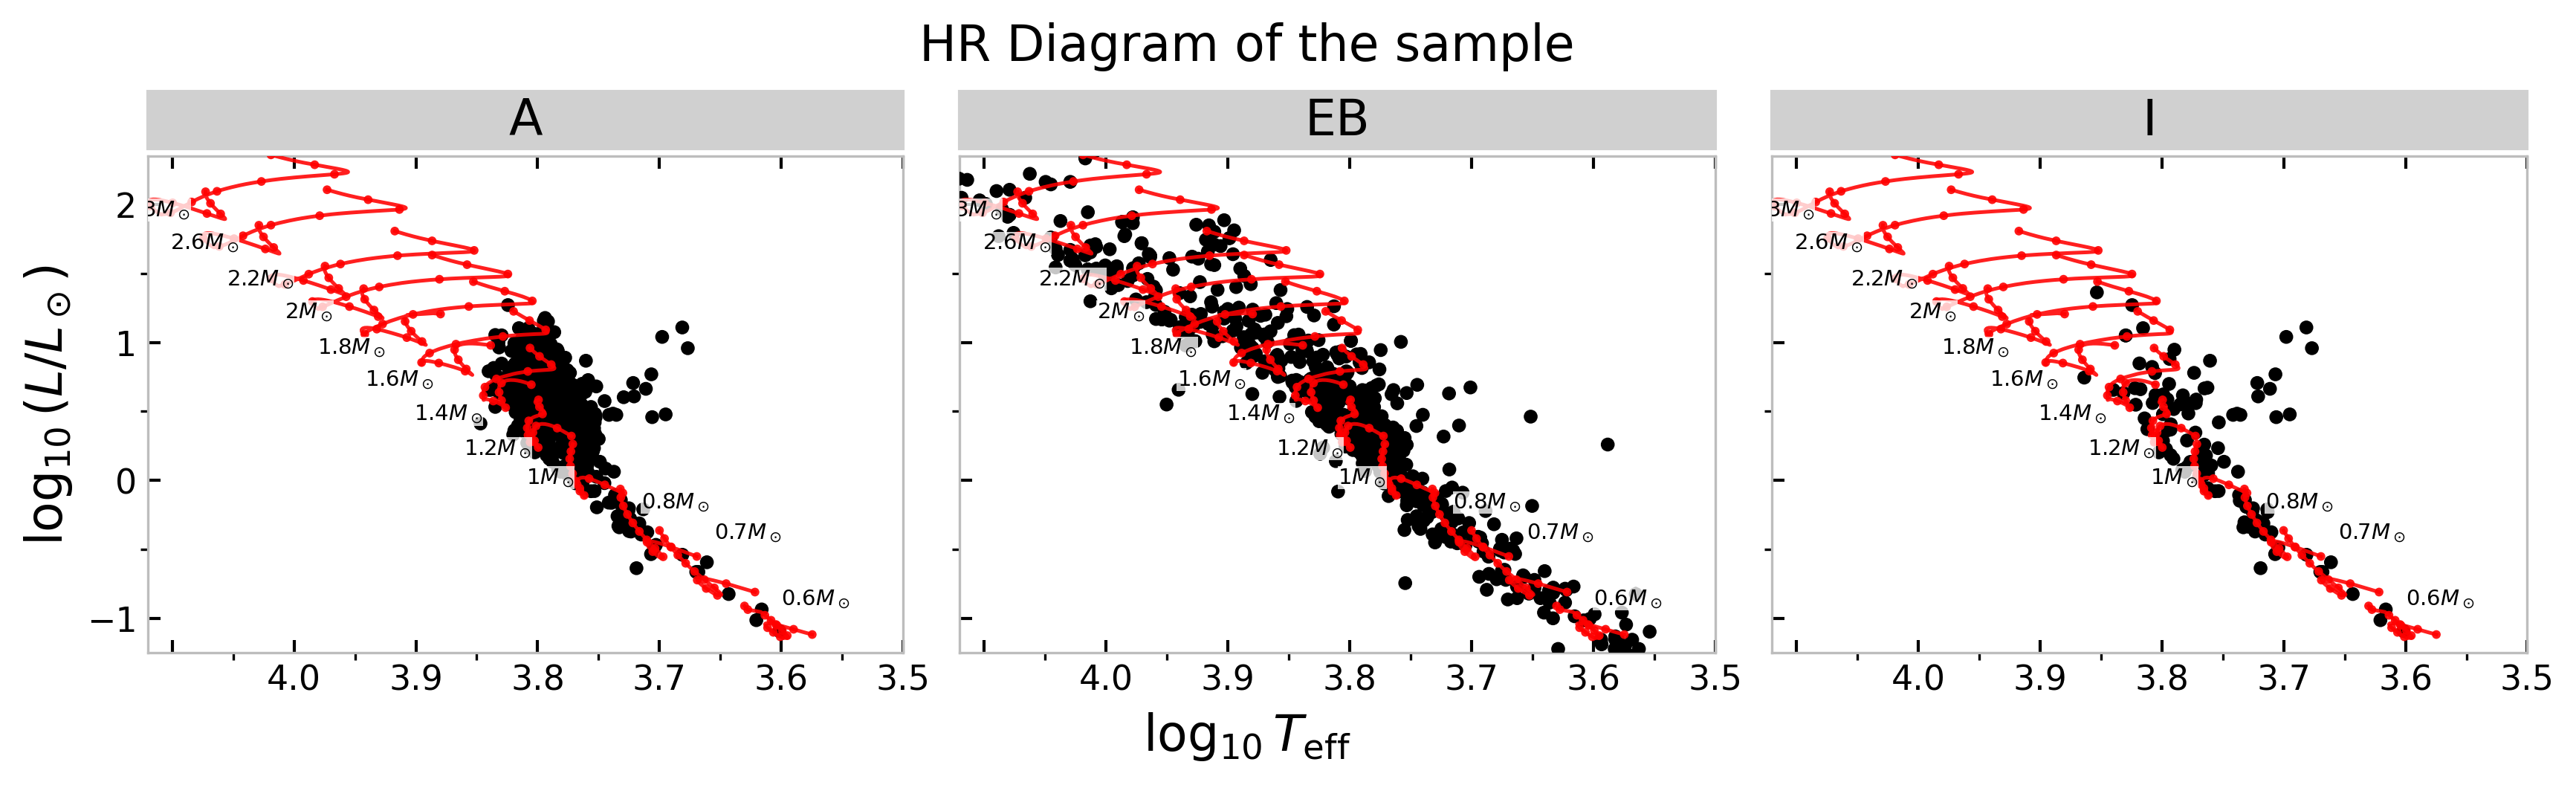
\includegraphics[width=0.99\linewidth]{hr_diagram_parsec_sample_clean.png}
    \caption{HR diagram of the 767 stars in the final sample. The red curves are theoretical evolutionary tracks of different masses obtained with PARSEC \citep{bressan2012}. The sample is divided by the main method used to study each star: asteroseismology, eclipsing binaries and interferometry.}
    \label{fig:HRdiagram}
\end{figure}

Finally, Section \ref{sec:dataset_C} requires the computation of oblateness (Equation \ref{eq:oblateness}), which depends on the orbital semi-major axis $a$. This parameter was often reported without an uncertainty. To retain a statistically meaningful sample, the missing uncertainty was estimated from four significant digits of the reported value. This produced 295 stars with computed oblateness, 48 of which used this uncertainty estimate.



\section{Machine Learning Model Training} \label{sec:results}
The behaviours and quantitative results described in these sections were consistent across different random-seed runs for the four analysed models, keeping the same inputs, target and training strategy. The main evaluation metrics are the Mean Absolute Error (MAE), which measures the average absolute difference between the true masses $m_i$ and the model estimates $\hat{m}_i$; the Mean Absolute Relative Difference (MARD), which measures the average relative accuracy across $N$ samples; and the Mean Relative Difference (MRD), which measures the signed relative bias of the predictions with respect to the true values.

\begin{equation}
\text{MAE} = \frac{\sum_{i=1}^N |m_i - \hat{m}_i|}{N}, \quad \text{MARD} = \frac{\sum_{i=1}^N \frac{|m_i - \hat{m}_i|}{m_i}}{N}, \quad \text{MRD} = \frac{\sum_{i=1}^N \frac{m_i - \hat{m}_i}{m_i}}{N}.
\end{equation}

\subsection{Mass Predictions for FGK-type Stars} \label{subsec:dataset_a}
Main-sequence stars of spectral types F, G and K are especially useful in stellar studies because they are common survey targets and therefore often have well-measured atmospheric parameters. By contrast, main-sequence M-type stars are less extensively documented. They are cooler, low-mass objects that burn hydrogen slowly and evolve very little over the age of the Universe \citep{laughlin1997}. Their intrinsic faintness and slow evolution make precise stellar parameters difficult to obtain \citep{chabrier2000}.

\citet{maxted2023benchmark} proposed a way to obtain information about M-type stars by studying eclipsing-binary systems in which the M star is the secondary component of a better-characterized primary star. Because many eclipsing-binary parameters are measured relative to the two components, information about one star can help constrain the other \citep{Southworth2015}. This motivates a focus on systems with an FGK-type primary and an M-type secondary: accurate mass predictions for the better-characterized FGK component can improve the inferred properties of the lower-mass companion. This helps to extend the calibration towards the M-star regime, where high-quality masses remain scarce.

As discussed in Section \ref{sec:cleaning}, Figure \ref{fig:HRdiagram} shows that the catalogue compiled in this work is rich in FGK-type stars, making this first mass-prediction experiment well suited to the available data. Following \citet{moya2018}, $T_{\mathrm{eff}}$, $\rho$ and $[\mathrm{Fe}/\mathrm{H}]$ were adopted as input parameters for stellar-mass estimation. This choice is motivated by well-studied eclipsing binaries, for which these quantities can be obtained more precisely than alternatives such as $\log g$ or $L$. After combining the stars compiled in this work with the Moya catalogue, applying the main-sequence selection described in Section \ref{sec:data}, requiring these three input parameters, and removing stars with zero reported uncertainty, the final available set contained 767 stars. Of these, 618 were used for training and the remaining 155 stars, corresponding to $20\%$, were retained as a holdout set for testing. The holdout set was repeatedly randomly selected for each seed run.

\subsubsection*{Results}

The behaviour described in this section was consistent across different random-seed runs for the four analysed models. The main evaluation metrics are the Mean Absolute Error (MAE), which measures the average absolute difference between the true masses $m_i$ and the model estimates $\hat{m}_i$; the Mean Absolute Relative Difference (MARD), which measures the average relative accuracy across $N$ samples; and the Mean Relative Difference (MRD), which measures the signed relative bias of the predictions with respect to the true values.

\begin{equation}
\text{MAE} = \frac{\sum_{i=1}^N |m_i - \hat{m}_i|}{N}, \quad \text{MARD} = \frac{\sum_{i=1}^N \frac{|m_i - \hat{m}_i|}{m_i}}{N}, \quad \text{MRD} = \frac{\sum_{i=1}^N \frac{m_i - \hat{m}_i}{m_i}}{N}.
\end{equation}

Figure \ref{fig:hbnn_mass_predictions} shows the HBNN mass predictions for one representative run. In the prediction panel, the points mostly follow the 1:1 relation between predicted and true mass. However, the distribution is not completely uniform: lower-mass stars tend to be overpredicted, whereas higher-mass stars tend to be underpredicted. When averaged over the full holdout set, these two effects partly cancel, leading to a Mean Relative Difference close to zero, $0.71\%$, as shown in Table \ref{tab:model_mard_mrd}.

This trend is more clearly visible in the residual plot\footnote{For visual clarity, residuals were defined as $M_{\mathrm{pred}}-M_{\mathrm{true}}$ in the figures, including \ref{fig:mass_holdout_all_models}, while in the MAE, MARD and MRD definitions the sign is switched, $M_{\mathrm{true}}-M_{\mathrm{pred}}$.}, Figure \ref{fig:hbnn_mass_residuals}. The residuals change sign at approximately $1.3\,M_\odot$: lower-mass stars tend to have positive residuals, while higher-mass stars tend to have negative residuals. Thus, HBNN performs well for the main, near-solar-mass population, where most predictions agree with $M_{\mathrm{true}}$ within $1\sigma$. The model should, however, be treated with caution outside this central region, especially for higher masses.

\begin{figure}[H]
\centering
\captionsetup[subfigure]{font=small}

% Top row: HBNN, GP
\begin{subfigure}[t]{0.24\textwidth}
    \centering
    
\includegraphics[width=\linewidth]{HBNN_mass_3param_L_1000_seed_225_full_prediction.png}
    \caption{HBNN prediction.}
    \label{fig:hbnn_mass_predictions}
\end{subfigure}
\hfill
\begin{subfigure}[t]{0.24\textwidth}
    \centering
    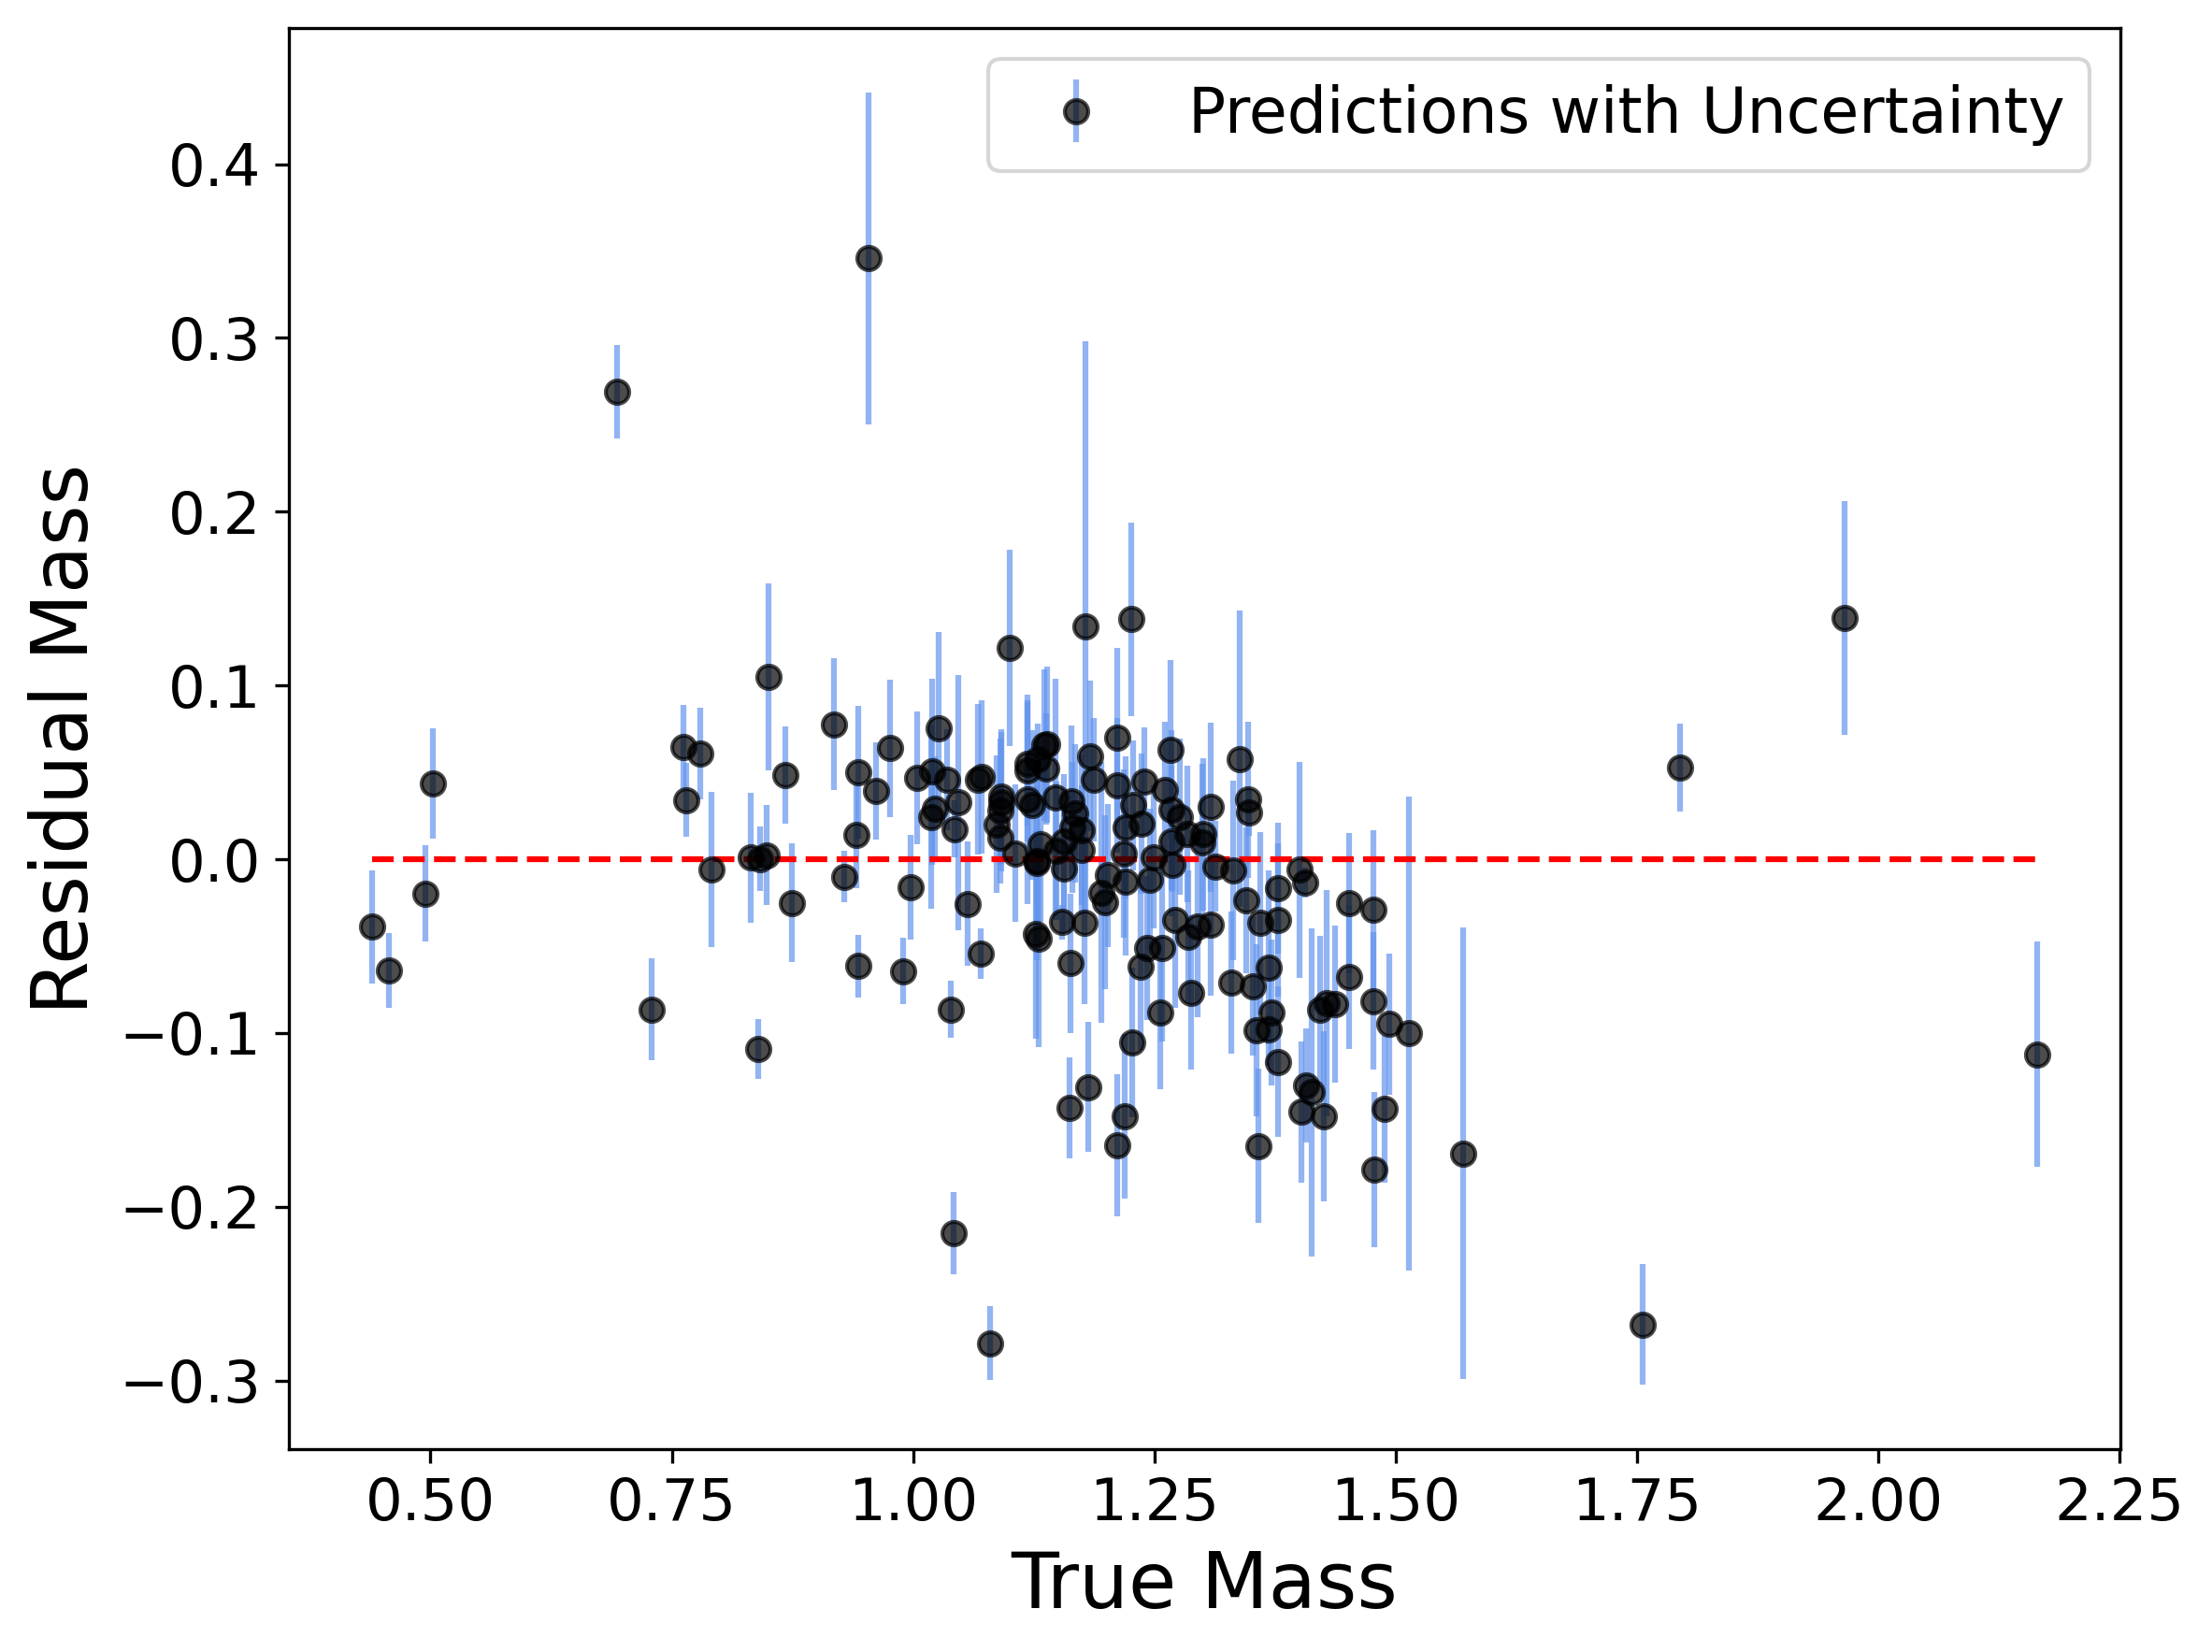
\includegraphics[width=\linewidth]{HBNN_mass_3param_L_1000_seed_225_full_residual.png}
    \caption{HBNN residuals.}
    \label{fig:hbnn_mass_residuals}
\end{subfigure}
\hfill
\begin{subfigure}[t]{0.24\textwidth}
    \centering
    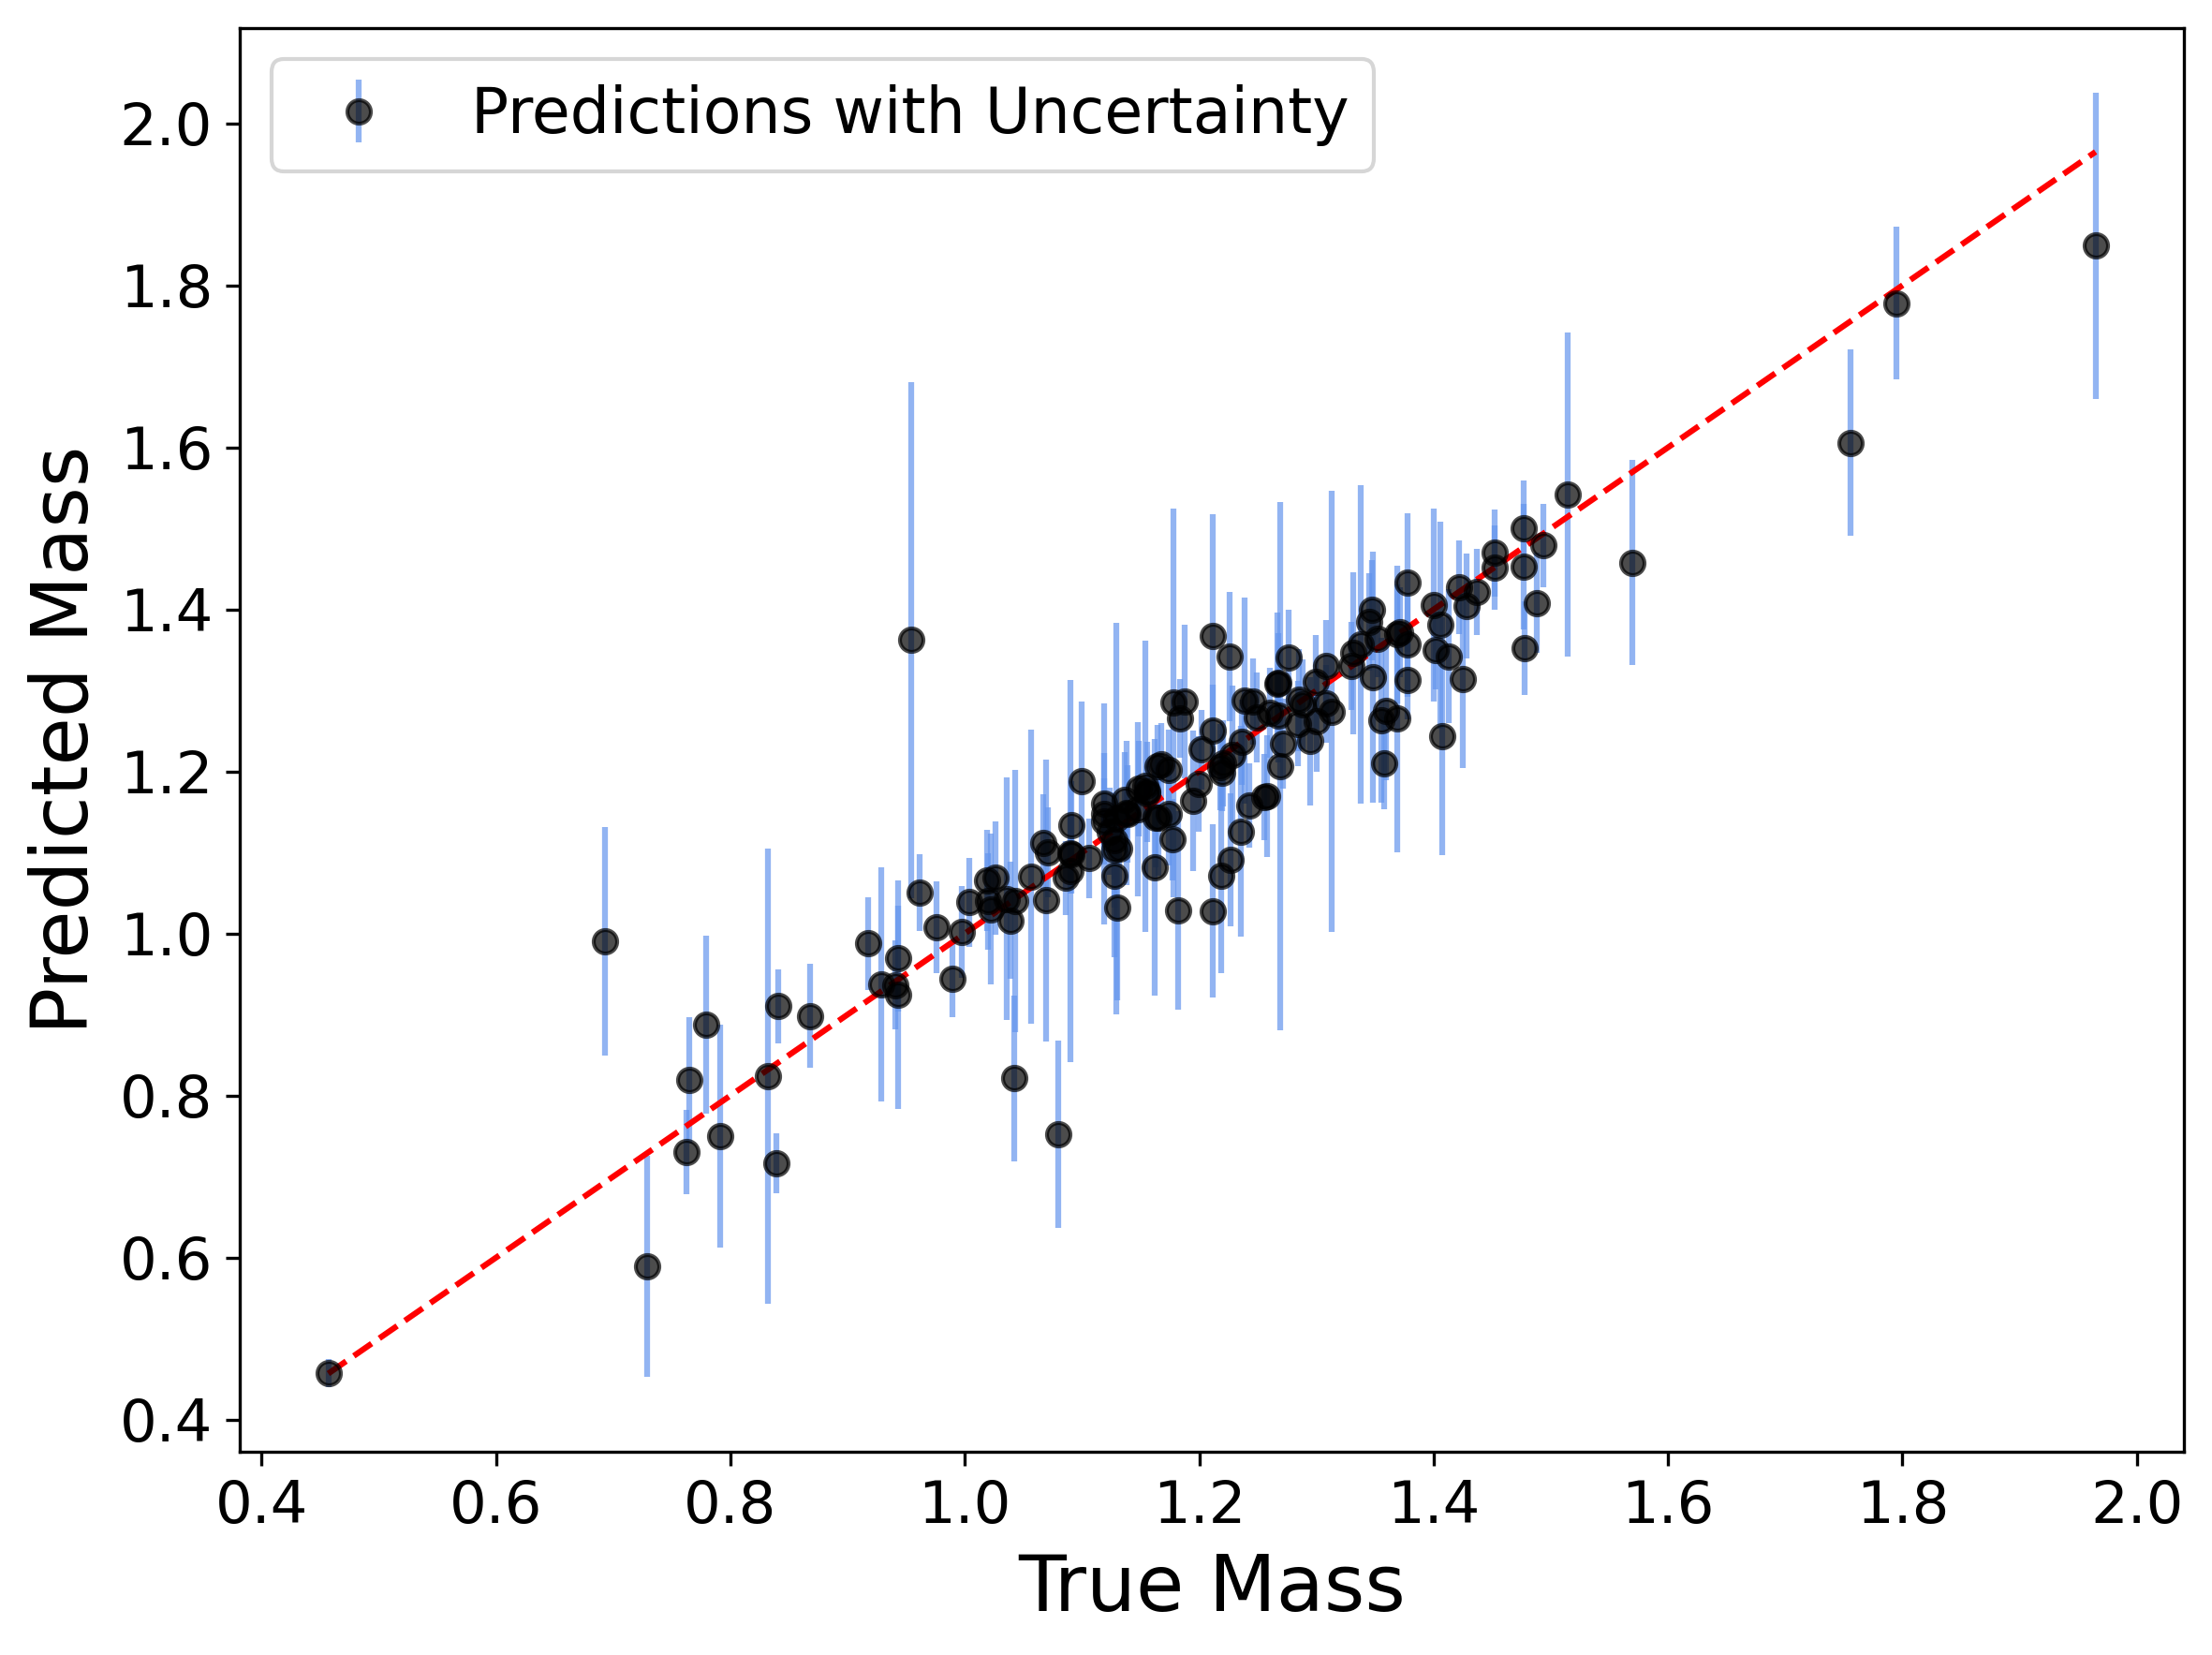
\includegraphics[width=\linewidth]{GP_mass_3param_L_1000_seed_225_filtered_95_prediction.png}
    \caption{GP prediction.}
    \label{fig:gp_mass_predictions}
\end{subfigure}
\hfill
\begin{subfigure}[t]{0.24\textwidth}
    \centering
    
\includegraphics[width=\linewidth]{GP_mass_3param_L_1000_seed_225_filtered_95_residual.png}
    \caption{GP residuals.}
    \label{fig:gp_mass_residuals}
\end{subfigure}

\vspace{0.4cm}

% Bottom row: BART, BHS
\begin{subfigure}[t]{0.24\textwidth}
    \centering
    
\includegraphics[width=\linewidth]{BART_mass_3param_L_prediction_seed_225_full_prediction.png}
    \caption{BART prediction.}
    \label{fig:bart_mass_predictions}
\end{subfigure}
\hfill
\begin{subfigure}[t]{0.24\textwidth}
    \centering
    
\includegraphics[width=\linewidth]{BART_mass_3param_L_prediction_seed_225_full_residual.png}
    \caption{BART residuals.}
    \label{fig:bart_mass_residuals}
\end{subfigure}
\hfill
\begin{subfigure}[t]{0.24\textwidth}
    \centering
    
\includegraphics[width=\linewidth]{BHS_mass_3param_L_prediction_seed_225_filtered_95_prediction.png}
    \caption{BHS prediction.}
    \label{fig:bhs_mass_predictions}
\end{subfigure}
\hfill
\begin{subfigure}[t]{0.24\textwidth}
    \centering
    
\includegraphics[width=\linewidth]{BHS_mass_3param_L_prediction_seed_225_filtered_95_residual.png}
    \caption{BHS residuals.}
    \label{fig:bhs_mass_residuals}
\end{subfigure}

\caption{Holdout-test performance of the HBNN, GP, BART and BHS mass models trained with $T_{\mathrm{eff}}$, $\rho$ and $[\mathrm{Fe}/\mathrm{H}]$. For each model, the prediction panel shows $M_{\mathrm{pred}}$ as a function of $M_{\mathrm{true}}$, while the residual panel shows $M_{\mathrm{pred}}-M_{\mathrm{true}}$ as a function of $M_{\mathrm{true}}$. Vertical error bars represent the predictive uncertainty returned by each model. The GP and BHS panels are restricted to the stars below the 95th percentile of predicted mass uncertainty in order to keep the main population visually readable. The full calibration sample contains $n=767$ stars, with $20\%$ reserved for the holdout test.}
\label{fig:mass_holdout_all_models}

\end{figure}

A plausible explanation is that the models were trained on a sample strongly concentrated around $1\,M_\odot$. As a result, HBNN tends to pull predictions towards this well-populated region, producing masses closer to the central training distribution than to the true values at the edges of the mass range. This behaviour is expected for Bayesian neural networks when the test inputs differ from the training distribution \citep{izmailov2021}.

The trend is less clear for the Gaussian Process model, as shown in Figure \ref{fig:gp_mass_predictions}. For visualization, the GP plots were restricted to stars with predicted mass uncertainty below the 95th percentile, because the full GP output contains a small number of objects with extremely large predicted uncertainties. Including those points compresses the vertical scale and makes the behaviour of the bulk of the sample unreadable.

Most GP predictions remain close to the 1:1 relation, and almost all points are compatible with the reference masses within $1\sigma$. The residual plot in Figure \ref{fig:gp_mass_residuals} shows a more compact and symmetric distribution around zero than the HBNN residuals in Figure \ref{fig:hbnn_mass_residuals}. This is also reflected in Table \ref{tab:model_mard_mrd}: the GP reaches a MARD of $4.79\%$, lower than the HBNN value of $5.27\%$. In addition, the GP has an MRD close to zero, $0.34\%$, indicating no clear global tendency to underpredict or overpredict stellar masses.


It is, however, notable that the GP uncertainties are larger than in the HBNN case, indicating that the model is underconfident in part of the sample. This remains true even after restricting the plotted set to the stars below the 95th percentile of predicted mass uncertainty. Stars with input-feature uncertainties larger than $9\%$ generated predicted mass uncertainties as large as $10^3\,M_\odot$, so they were removed from the sample, in order to investigate the origin of this extremely underconfident behaviour. This removed 17 objects, but did not eliminate the problem. 

In sparse regions of the input space, Gaussian Processes naturally return broader predictive distributions, reflecting extrapolation uncertainty \citep{cho2026}. This is one of the main advantages of GPs: predictive uncertainty increases when the model has little nearby information. This explains why no strong systematic trend is visible in Figures \ref{fig:gp_mass_predictions} and \ref{fig:gp_mass_residuals}. However, the very large uncertainty values found here, sometimes of order $10^2$--$10^3\,M_\odot$, are not physically meaningful.

A further inspection of the objects with very large predicted uncertainties, after removing those stars with input parameter uncertainties larger than $9\%$, showed that these input objects were no longer the same across different runs, and no physical pattern was found in their stellar parameters. This suggests that the issue is not only caused by a few erroneous data entries, but is likely connected to instability in the GP posterior or in the variance submodel. \citet{le2005heteroscedasticgp} discuss GP regression with input-dependent noise and note that directly estimating both the mean and the variance leads to difficult optimisation problems. For this reason, the GP results should be interpreted with caution. The percentile-restricted plots are used only to display the behaviour of the main population, not to hide the existence of these unstable uncertainty estimates.

For BART, Figures \ref{fig:bart_mass_predictions} and \ref{fig:bart_mass_residuals}, the result is similar to that obtained with the Bayesian neural-network model: masses below $1\,M_\odot$ tend to be overpredicted, while masses above $1\,M_\odot$ tend to be underpredicted. The predictions remain relatively close to the 1:1 relation, yielding a low MARD value of $4.98\%$. The negative MRD value, $-0.63\%$, shows that low-mass overpredictions and high-mass underpredictions again partially cancel when averaged across the full data interval. Therefore, as in the HBNN case, the MRD alone is not sufficient to describe the model behaviour unless it is interpreted together with the prediction and residual plots.

Here, the reduced accuracy outside the central training region is consistent with a known limitation of tree-based regression models. Standard BART and related tree ensembles are strong interpolators, but their extrapolation ability is limited by their leaf-based, piecewise-constant structure. Predictions outside sparsely sampled regions can become biased towards the dominant range of the training data and may have poorly calibrated uncertainty \citep{zhang2019rerf}. BART also shows comparatively large uncertainties, so the loss of accuracy away from the central mass range is reflected in underconfident predictions.

Finally, the stacking model was applied to combine the information contained in the individual BART, GP and HBNN predictions. Since both HBNN and BART show systematic behaviour away from the region near $1\,M_\odot$, the GP model is expected to have a larger influence in those outer regions. Therefore, the BHS plots shown in Figures \ref{fig:bhs_mass_predictions} and \ref{fig:bhs_mass_residuals} are also restricted to stars below the 95th percentile of predicted mass uncertainty, avoiding the visual masking produced by a small number of extremely uncertain points.

Figure \ref{fig:bhs_mass_predictions} shows no clear mass-dependent trend in the BHS predictions. Therefore, the systematic mispredictions observed for BART and HBNN away from one solar mass are not inherited by the stacking model. The resulting MRD value, $0.29\%$, is close to zero and is the lowest among the four models, supporting the absence of a visible global bias. In this case, the behaviour of the plots confirms that the near-zero MRD is not mainly produced by localized overpredictions and underpredictions cancelling each other out, as happened for HBNN and BART.

Although the GP model clearly influences BHS, since the negative-slope trend is no longer visible, the difference between the BHS MARD, $4.66\%$, and the GP MARD, $4.79\%$, shows that the stacking model is not simply mimicking the GP model overall. Instead, it combines the models in a way that improves the final residual metrics while reducing the systematic behaviour seen in some of the individual predictors.

The predictive uncertainties observed in the plots of the BHS model are, however, the largest among the models in this representative run. This is consistent with the fact that stacking combines predictive distributions from all models and can inherit part of the large uncertainties that both the GP and BART components show for some stars \citep{yao2022hierarchicalstacking}.

\begin{table}[H]
\centering
\caption{Comparison of the residual metrics obtained by the mass-prediction models on the holdout set. The models were trained with $T_{\mathrm{eff}}$, $\rho$ and $[\mathrm{Fe}/\mathrm{H}]$ as input features, and stellar mass as the target.}
\label{tab:model_mard_mrd}
\begin{tabular}{lcccc}
\hline\hline
Metric & BART & GP & HBNN & BHS \\
\hline
MAE ($M_\odot$) & $0.057$ & $0.053$ & $0.060$ & $0.052$ \\
MARD [\%] & $4.98$ & $4.79$ & $5.27$ & $4.66$ \\
MRD [\%]  & $-0.63$ & $0.34$ & $0.71$ & $0.29$ \\
\hline
\end{tabular}
\end{table}

% Training for 3 features, target mass, old dataset:
% MARD BART: 4.012486991522741
% MRD BART: -0.22293463827194457
% MARD GP: 3.5874216150037346
% MRD GP: 0.14603481547699454
% MARD HBNN: 3.8129161602457264
% MRD HBNN: 0.30524703057713803
% MARD BHS: 3.595270798056581
% MRD BHS: 0.01995748961690648

% Old file: about 423 training rows after split
% New file: 810 usable MS rows total -> about 648 training rows after 80/20 split

The evaluation metrics (Table \ref{tab:model_mard_mrd}) show that, overall, the relative errors are consistently around the $5\%$ level, which is a strong result for this calibration sample. Similar values were obtained by the BHS model presented by \citet{moya2022}. However, that model used four input features instead of three, and would therefore have access to more predictive information, as discussed by those authors. The 2022 model did not propagate the observational uncertainties of the stellar parameters. The fact that the present three-feature models reach comparable MARD values while incorporating these uncertainties suggests that the improved probabilistic treatment provides a more robust calibration withour a clear loss of predictive accuracy.

This interpretation is also supported by the MAE comparison. \citet{moya2022} reported a stacking-model MAE of $0.048\,M_\odot$, which is very close to the BHS value of $0.052\,M_\odot$ obtained here. Considering the remaining models presented by \citet{moya2022}, with MAE values in the range $0.06$--$0.08\,M_\odot$, the models in this work achieve lower absolute errors in all cases, while treating the reported input uncertainties consistently.

Finally, all MRD values are below $1\%$. For GP and BHS, this is consistent with the absence of a clear global bias in the prediction plots. For HBNN and BART, however, the near-zero MRD should not be interpreted alone: in those cases, it is mainly a consequence of systematic overpredictions and underpredictions cancelling when averaged over the full holdout set.

\subsection{ARIEL: Model-independent predictions} \label{subsec:dataset_b}

ARIEL, the Atmospheric Remote-sensing Infrared Exoplanet Large-survey, is ESA's fourth medium-class mission, M4, within the Cosmic Vision programme, and is planned for launch around 2030. It is dedicated to the atmospheric characterization of exoplanets and will study the chemical composition of the atmospheres of approximately 1000 transiting planets. The mission is based on spectroscopic and photometric observations, where the planetary signal is measured relative to the emission of the host star. Accurate and homogeneous stellar characterisation is therefore essential for the interpretation of ARIEL observations.

Within this context, the Age, Mass and Radius sub-working group aims to provide homogeneous estimates of stellar ages, masses and radii for the ARIEL target stars \citep{arielAMRsubwg}. The Astronomy and Astrophysics Department at the Universitat de València manages this stellar characterization working group. The task is approached through complementary implementations, including both stellar-modelling methods and data-driven ML/AI techniques. The former implementation is supported by the Astrophysics and Space Sciences Institute of the Universidade do Porto.

Surface gravity, $g$, is a physically informative quantity for the estimation of stellar masses and radii. Previous empirical and machine-learning studies have shown that its inclusion can improve predictive performance \citep{moya2018}. However, $g$ is often determined through procedures that depend on stellar models. Using it as an input feature in the data-driven model would therefore reduce the independence between the two complementary approaches considered in the ARIEL stellar-characterization work. For this reason, the models in this section were trained using $T_{\mathrm{eff}}$, $[\mathrm{Fe}/\mathrm{H}]$ and $L$ as input features. These quantities are not completely free from methodological assumptions, but they avoid the same direct dependence on stellar evolutionary models.

The procedure described in Section \ref{subsec:dataset_a} was then repeated using this updated set of input features, yielding similar results, both visually and quantitatively. In this case, however, an additional comparison was possible. The Institute of Astrophysics of the Universidade do Porto provided a complementary dataset of stellar masses obtained through stellar-modelling methods. These estimates are based on PARSEC, the PAdova and TRieste Stellar Evolution Code, which provides stellar evolutionary tracks and isochrones used to infer stellar properties from theoretical models \citep{bressan2012}. This dataset was first cleaned to remove stars that had already been used during training, and was then used to obtain mass predictions with the trained models. The new mass predictions, including their uncertainties, were compared with the masses obtained from stellar evolutionary grids. Linear relations developed by \citet{moya2018} were added to the comparison as well. This provides a benchmark against both model-based mass estimates and previously published data-driven mass-estimation methods.
\subsubsection*{Results}
The evaluations against the $20\%$ holdout test were performed using the MAE, MARD and MRD indicators introduced in Section \ref{subsec:dataset_a}. Table \ref{tab:dataset_b_mard_mrd} shows that the behaviour of the models is consistent with that found when training with $\rho$ instead of $L$, although the performance is slightly worse, with MARD values increasing by about two percentage points. This supports the conclusion of \citet{moya2018} that $\rho$ is a particularly informative parameter for stellar-mass prediction. Nevertheless, Figure \ref{fig:mass_holdout_all_models_B} puts this loss of accuracy into context, since the points remain only moderately dispersed around the 1:1 relation. Even with this decrease in performance, the results remain acceptable for the purposes of this comparison; the MAE values obtained, all within the range $0.07$--$0.08\,M_\odot$, are comparable to those reported for different models by \citet{moya2022}, which lie within the range $0.06$--$0.08\,M_\odot$.

\begin{table}[H]
\centering
\caption{Comparison of the residual metrics obtained by the mass-prediction models on the holdout set. The models were trained with $T_{\mathrm{eff}}$, $L$ and $[\mathrm{Fe}/\mathrm{H}]$ as input features, and stellar mass as the target.}
\label{tab:dataset_b_mard_mrd}
\begin{tabular}{lcccc}
\hline\hline
Metric & BART & GP & HBNN & BHS \\
\hline
MAE ($M_\odot$) & $0.076$ & $0.077$ & $0.074$ & $0.072$ \\
MARD [\%] & $6.99$ & $6.79$ & $7.02$ & $6.53$ \\
MRD [\%]  & $-2.39$ & $-1.14$ & $-1.89$ & $-1.36$ \\
\hline
\end{tabular}
\end{table}

GP is the level-0 model with the best MRD value, while BART and HBNN show signs of systematic misprediction. For HBNN, the tendency of the model to shift masses towards values close to $1.25\,M_\odot$ is still visible in Figure \ref{fig:hbnn_mass_residuals_B}, although the MRD value of $-1.89\%$ shows that overpredictions are more common. These mispredictions were expected, since the training set was not expanded and some regions of parameter space remain poorly represented. The same behaviour is also found for BART, which reaches an even more negative MRD of $-2.39\%$. BART also returns comparatively large uncertainties in these regions.

The GP model also shows underconfident behaviour. The plots must therefore be trimmed to the 95th percentile of predicted mass uncertainty to prevent a small number of outliers with very large uncertainties from masking the population. The indicators in Table \ref{tab:dataset_b_mard_mrd} suggest a slight trend towards overprediction, while Figure \ref{fig:gp_mass_residuals_B} shows that this corresponds to a modest positive offset that remains approximately constant across the $M_{\mathrm{true}}$ axis.

\begin{figure}[H]
\centering
\captionsetup[subfigure]{font=small}

% Top row: HBNN, GP
\begin{subfigure}[t]{0.24\textwidth}
\centering
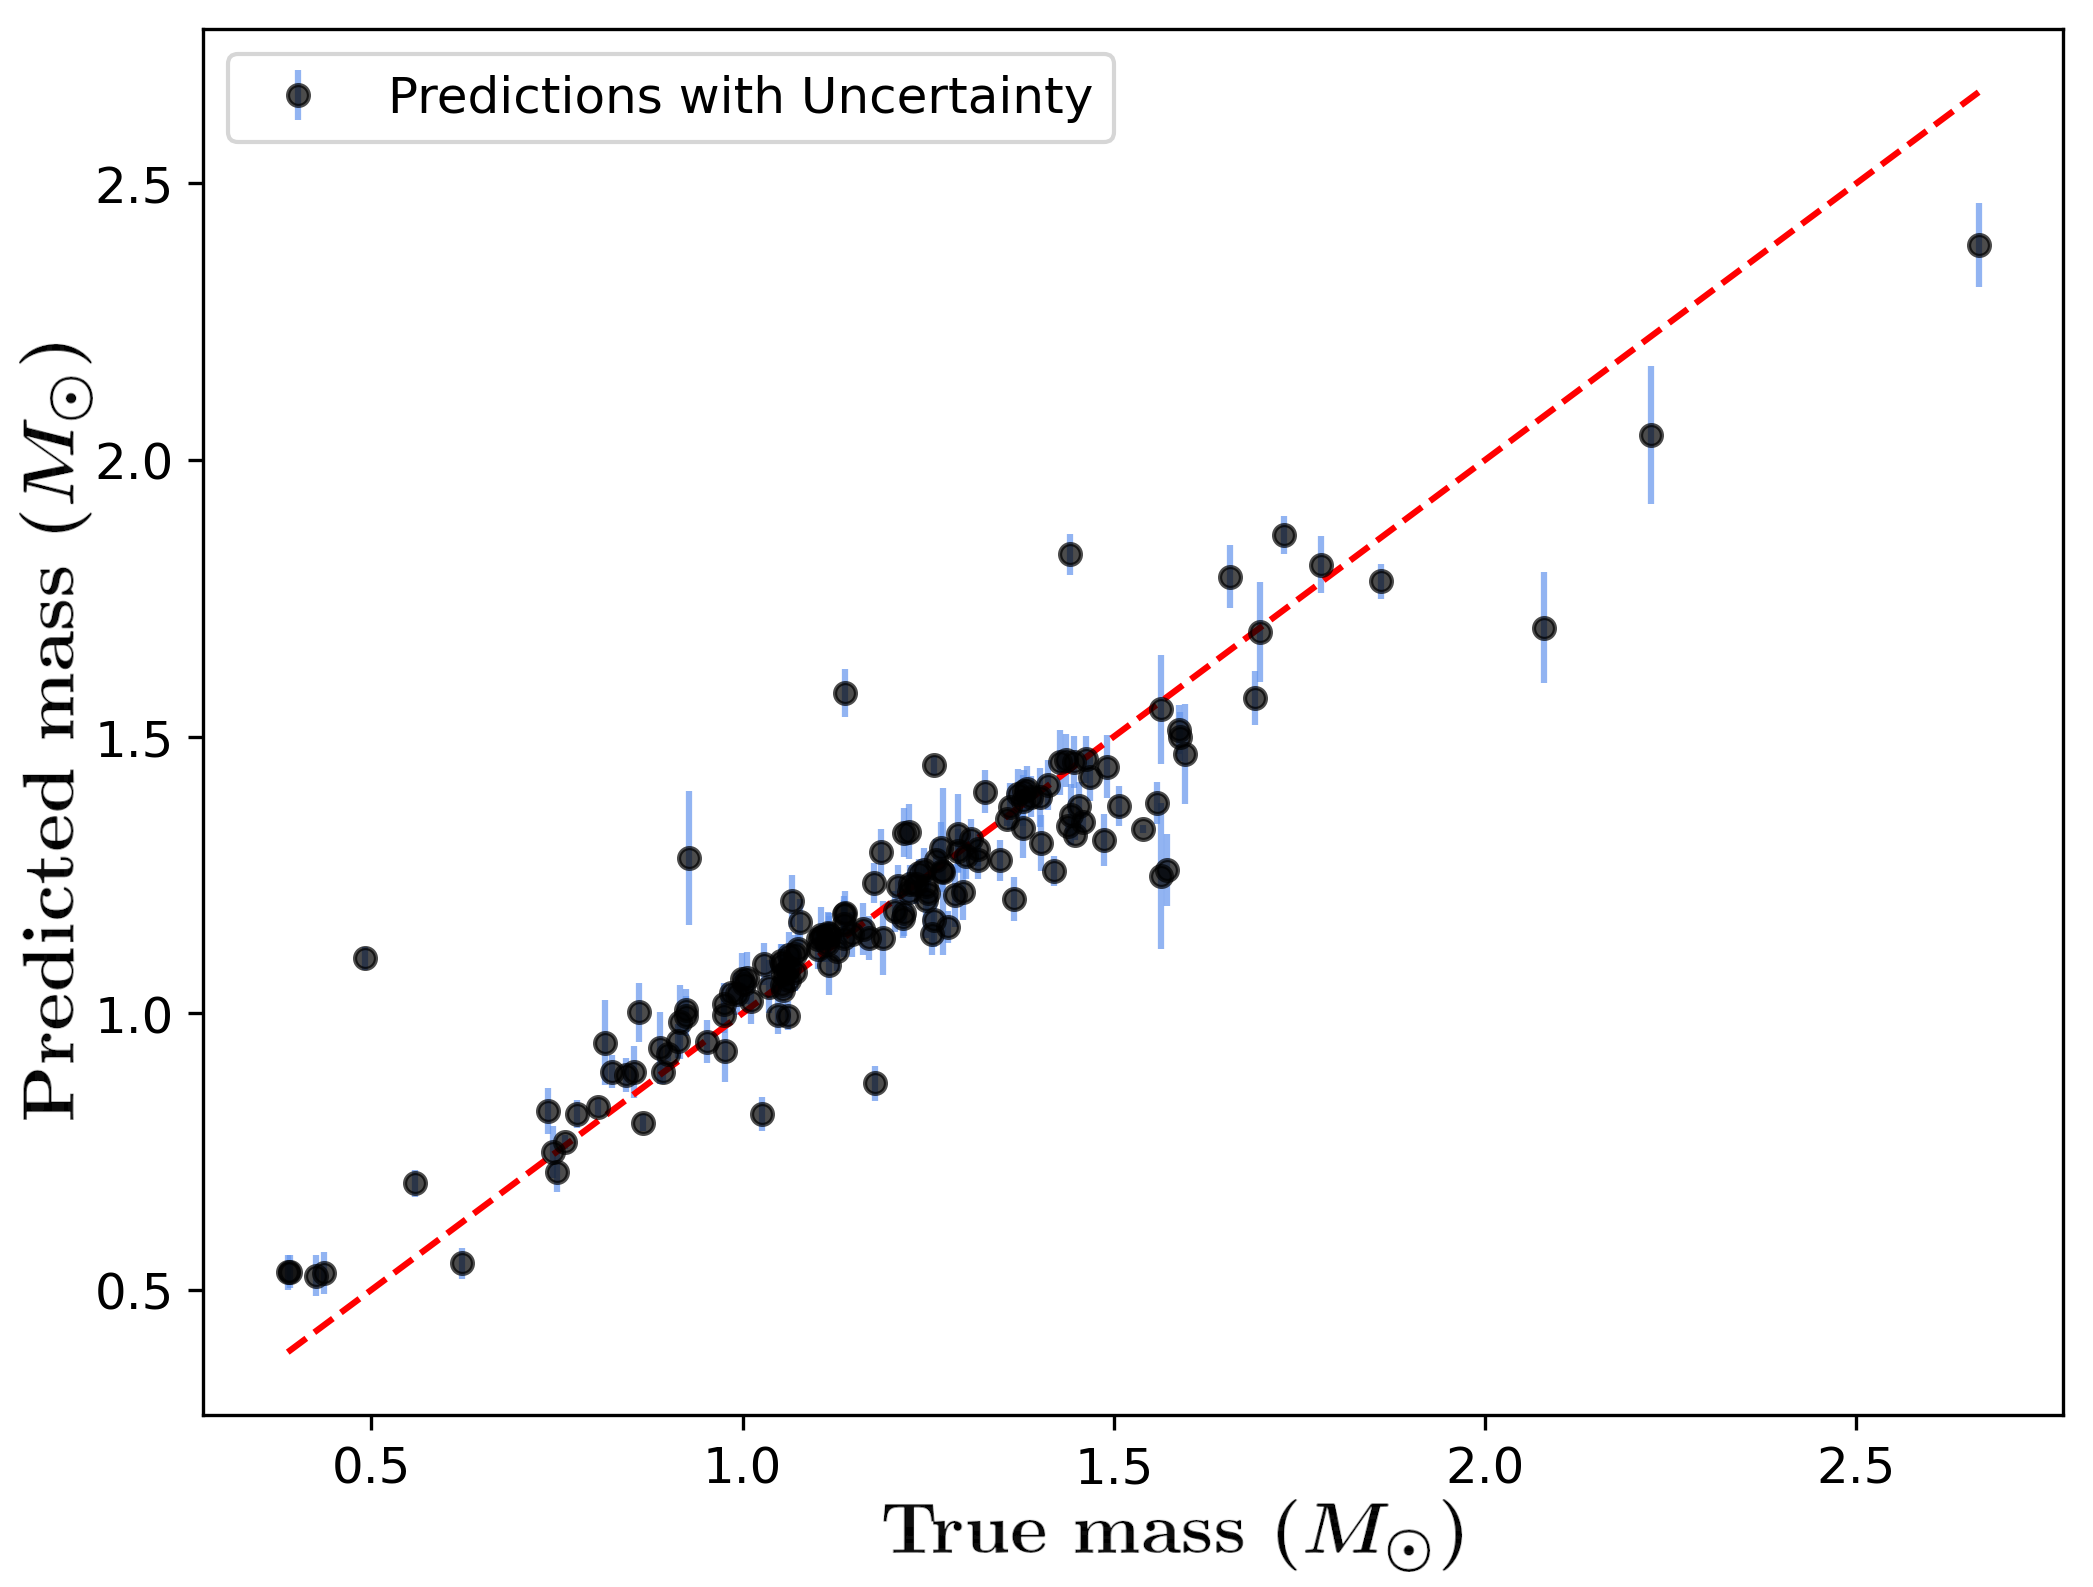
\includegraphics[width=\linewidth]{HBNN_mass_3param_L_1000_draws_4_chains_15_nodes_sig_015_seed_176_full_prediction_no_title_smaller_points_fontplus2.png}
\caption{HBNN prediction.}
\label{fig:hbnn_mass_predictions_B}
\end{subfigure}
\hfill
\begin{subfigure}[t]{0.24\textwidth}
\centering
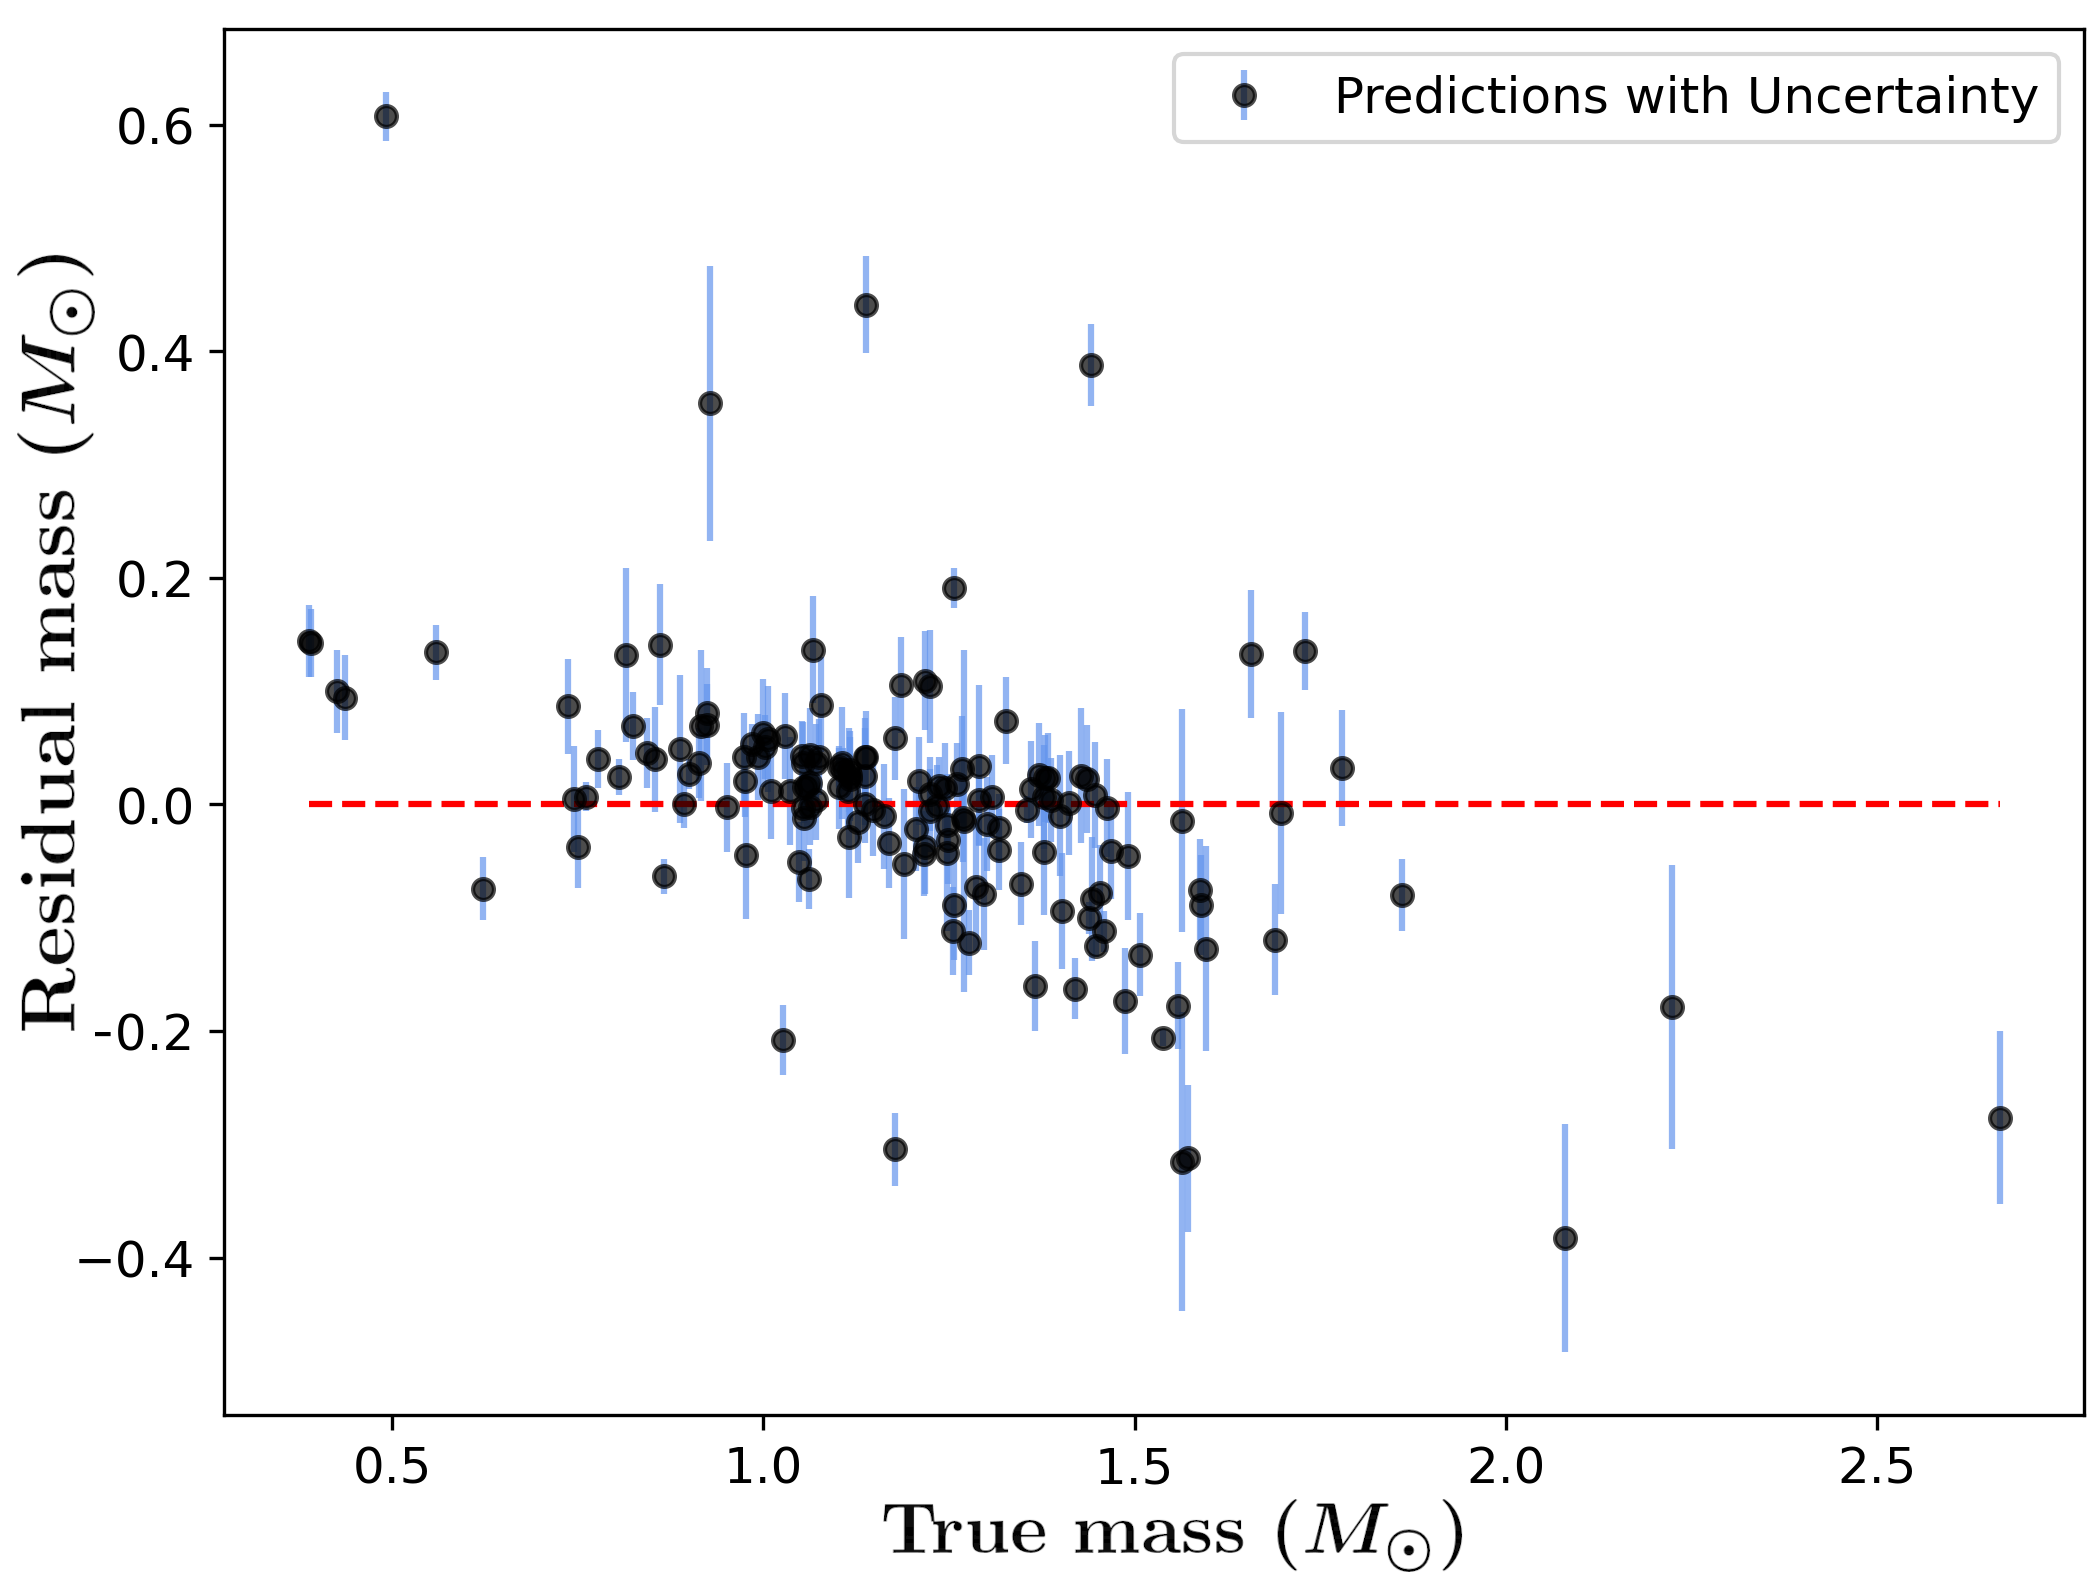
\includegraphics[width=\linewidth]{HBNN_mass_3param_L_1000_draws_4_chains_15_nodes_sig_015_seed_176_full_residual_no_title_smaller_points_fontplus2.png}
\caption{HBNN residuals.}
\label{fig:hbnn_mass_residuals_B}
\end{subfigure}
\hfill
\begin{subfigure}[t]{0.24\textwidth}
\centering
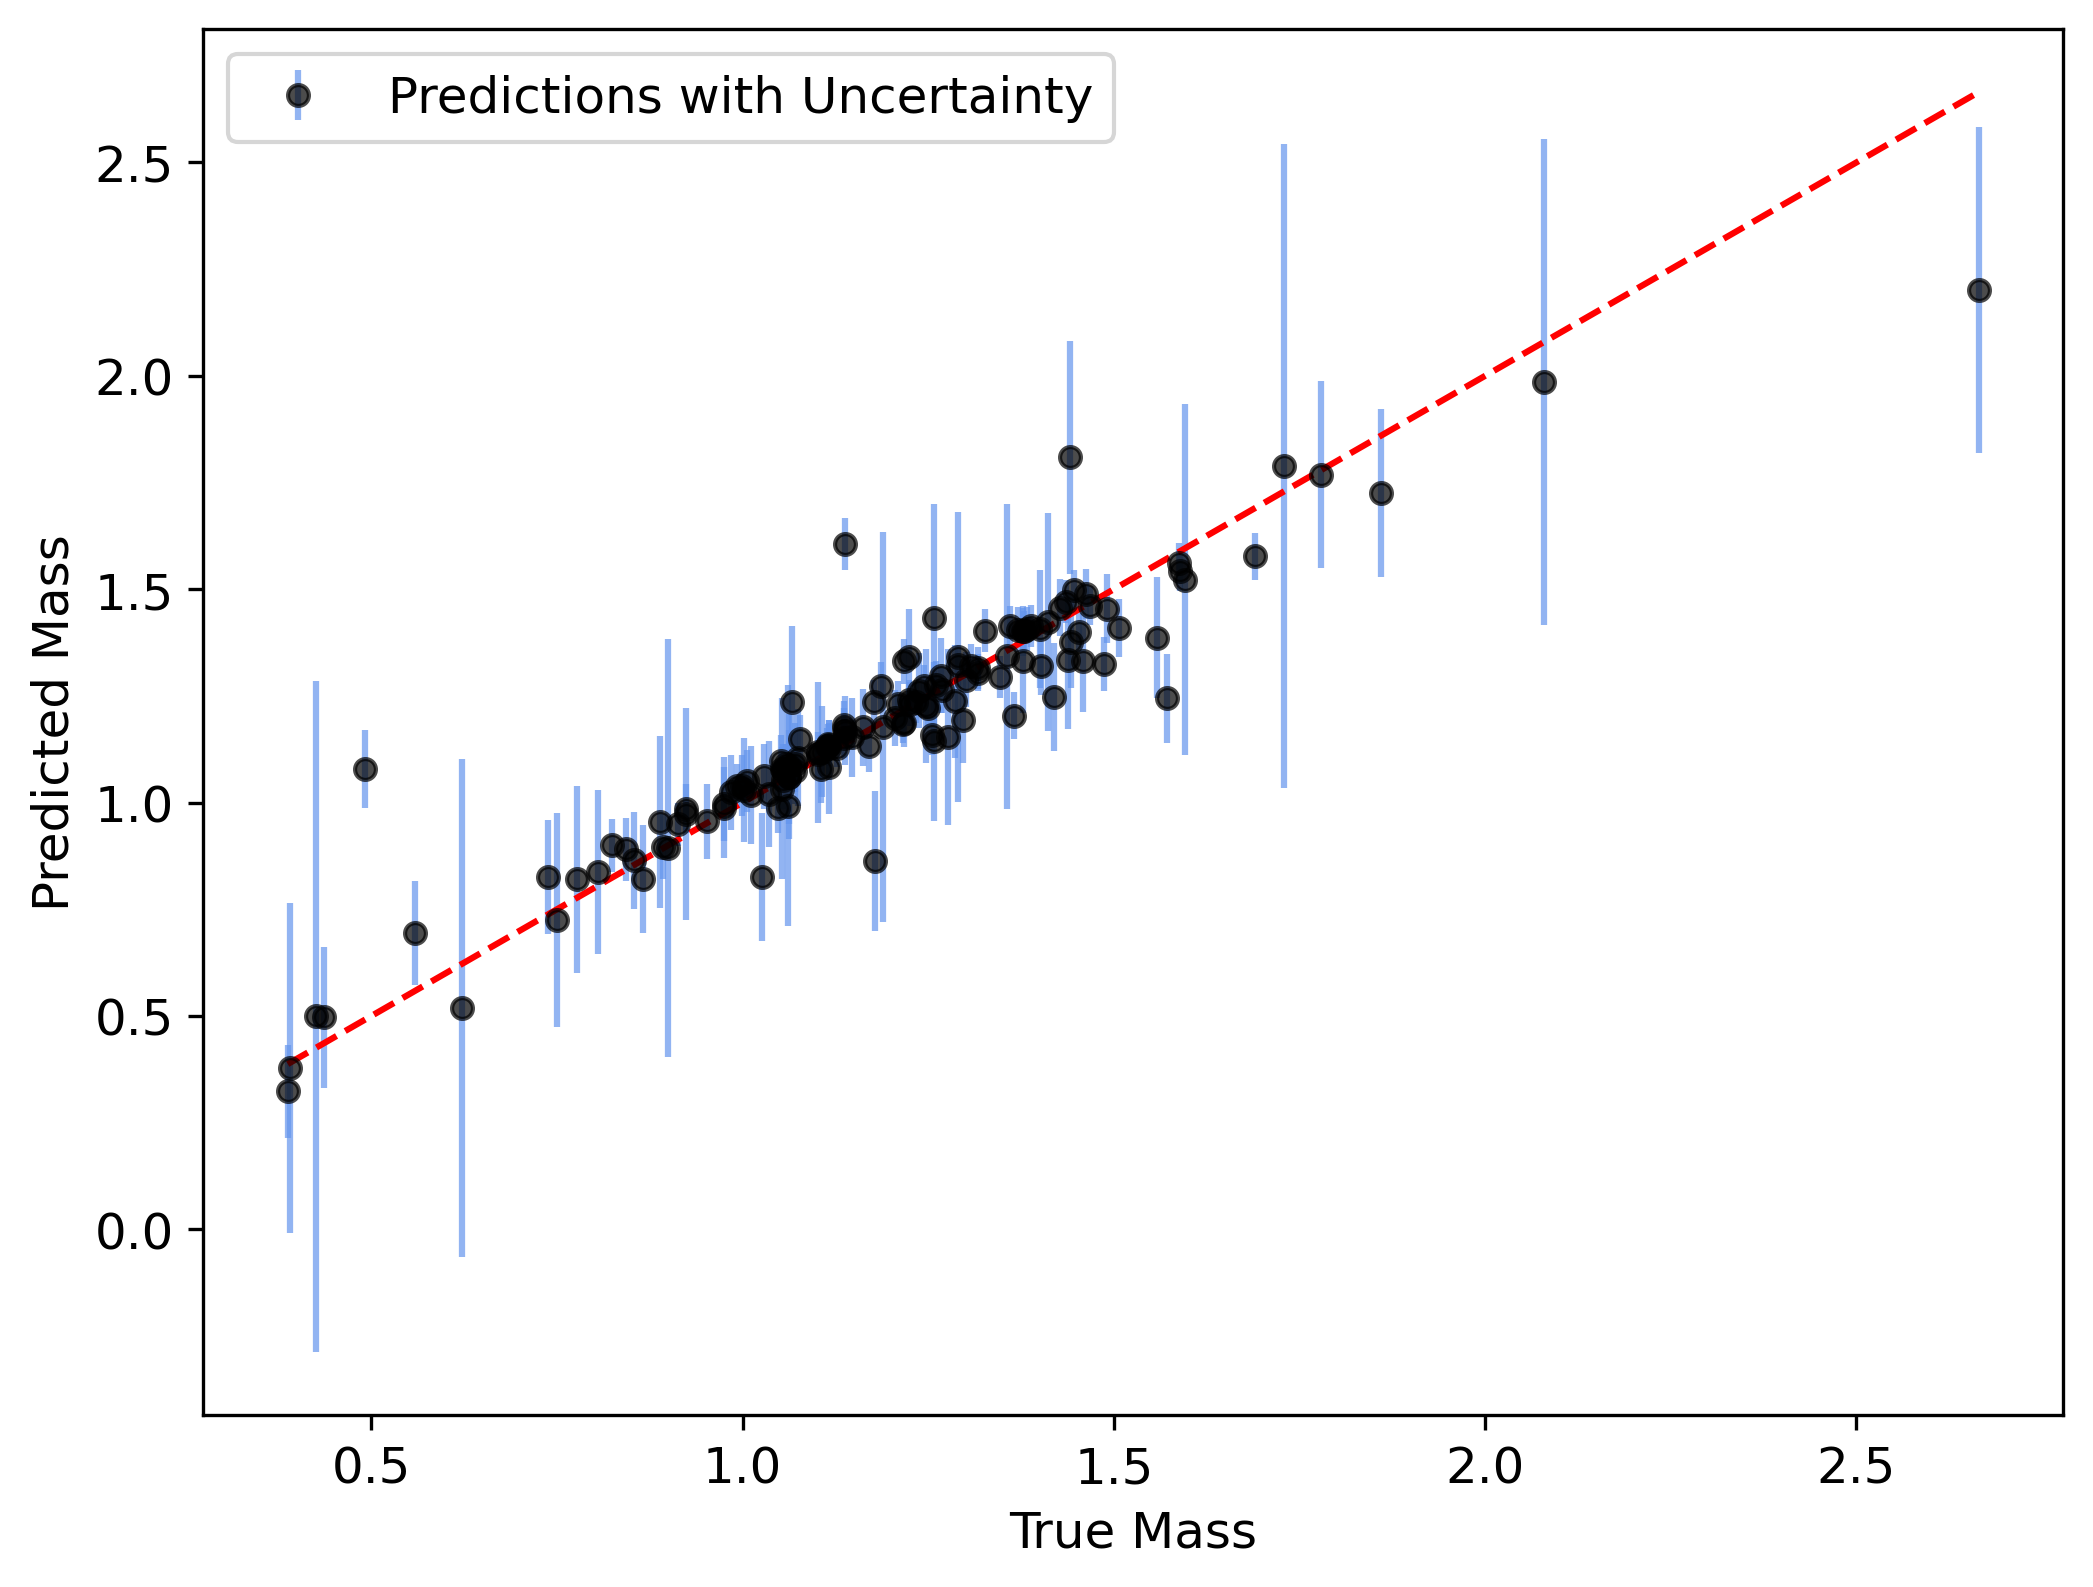
\includegraphics[width=\linewidth]{GP_mass_3param_L_1000_draws_4_chains_80_40_seed_176_filtered_90_prediction_no_title_smaller_points_fontplus2.png}
\caption{GP prediction.}
\label{fig:gp_mass_predictions_B}
\end{subfigure}
\hfill
\begin{subfigure}[t]{0.24\textwidth}
\centering
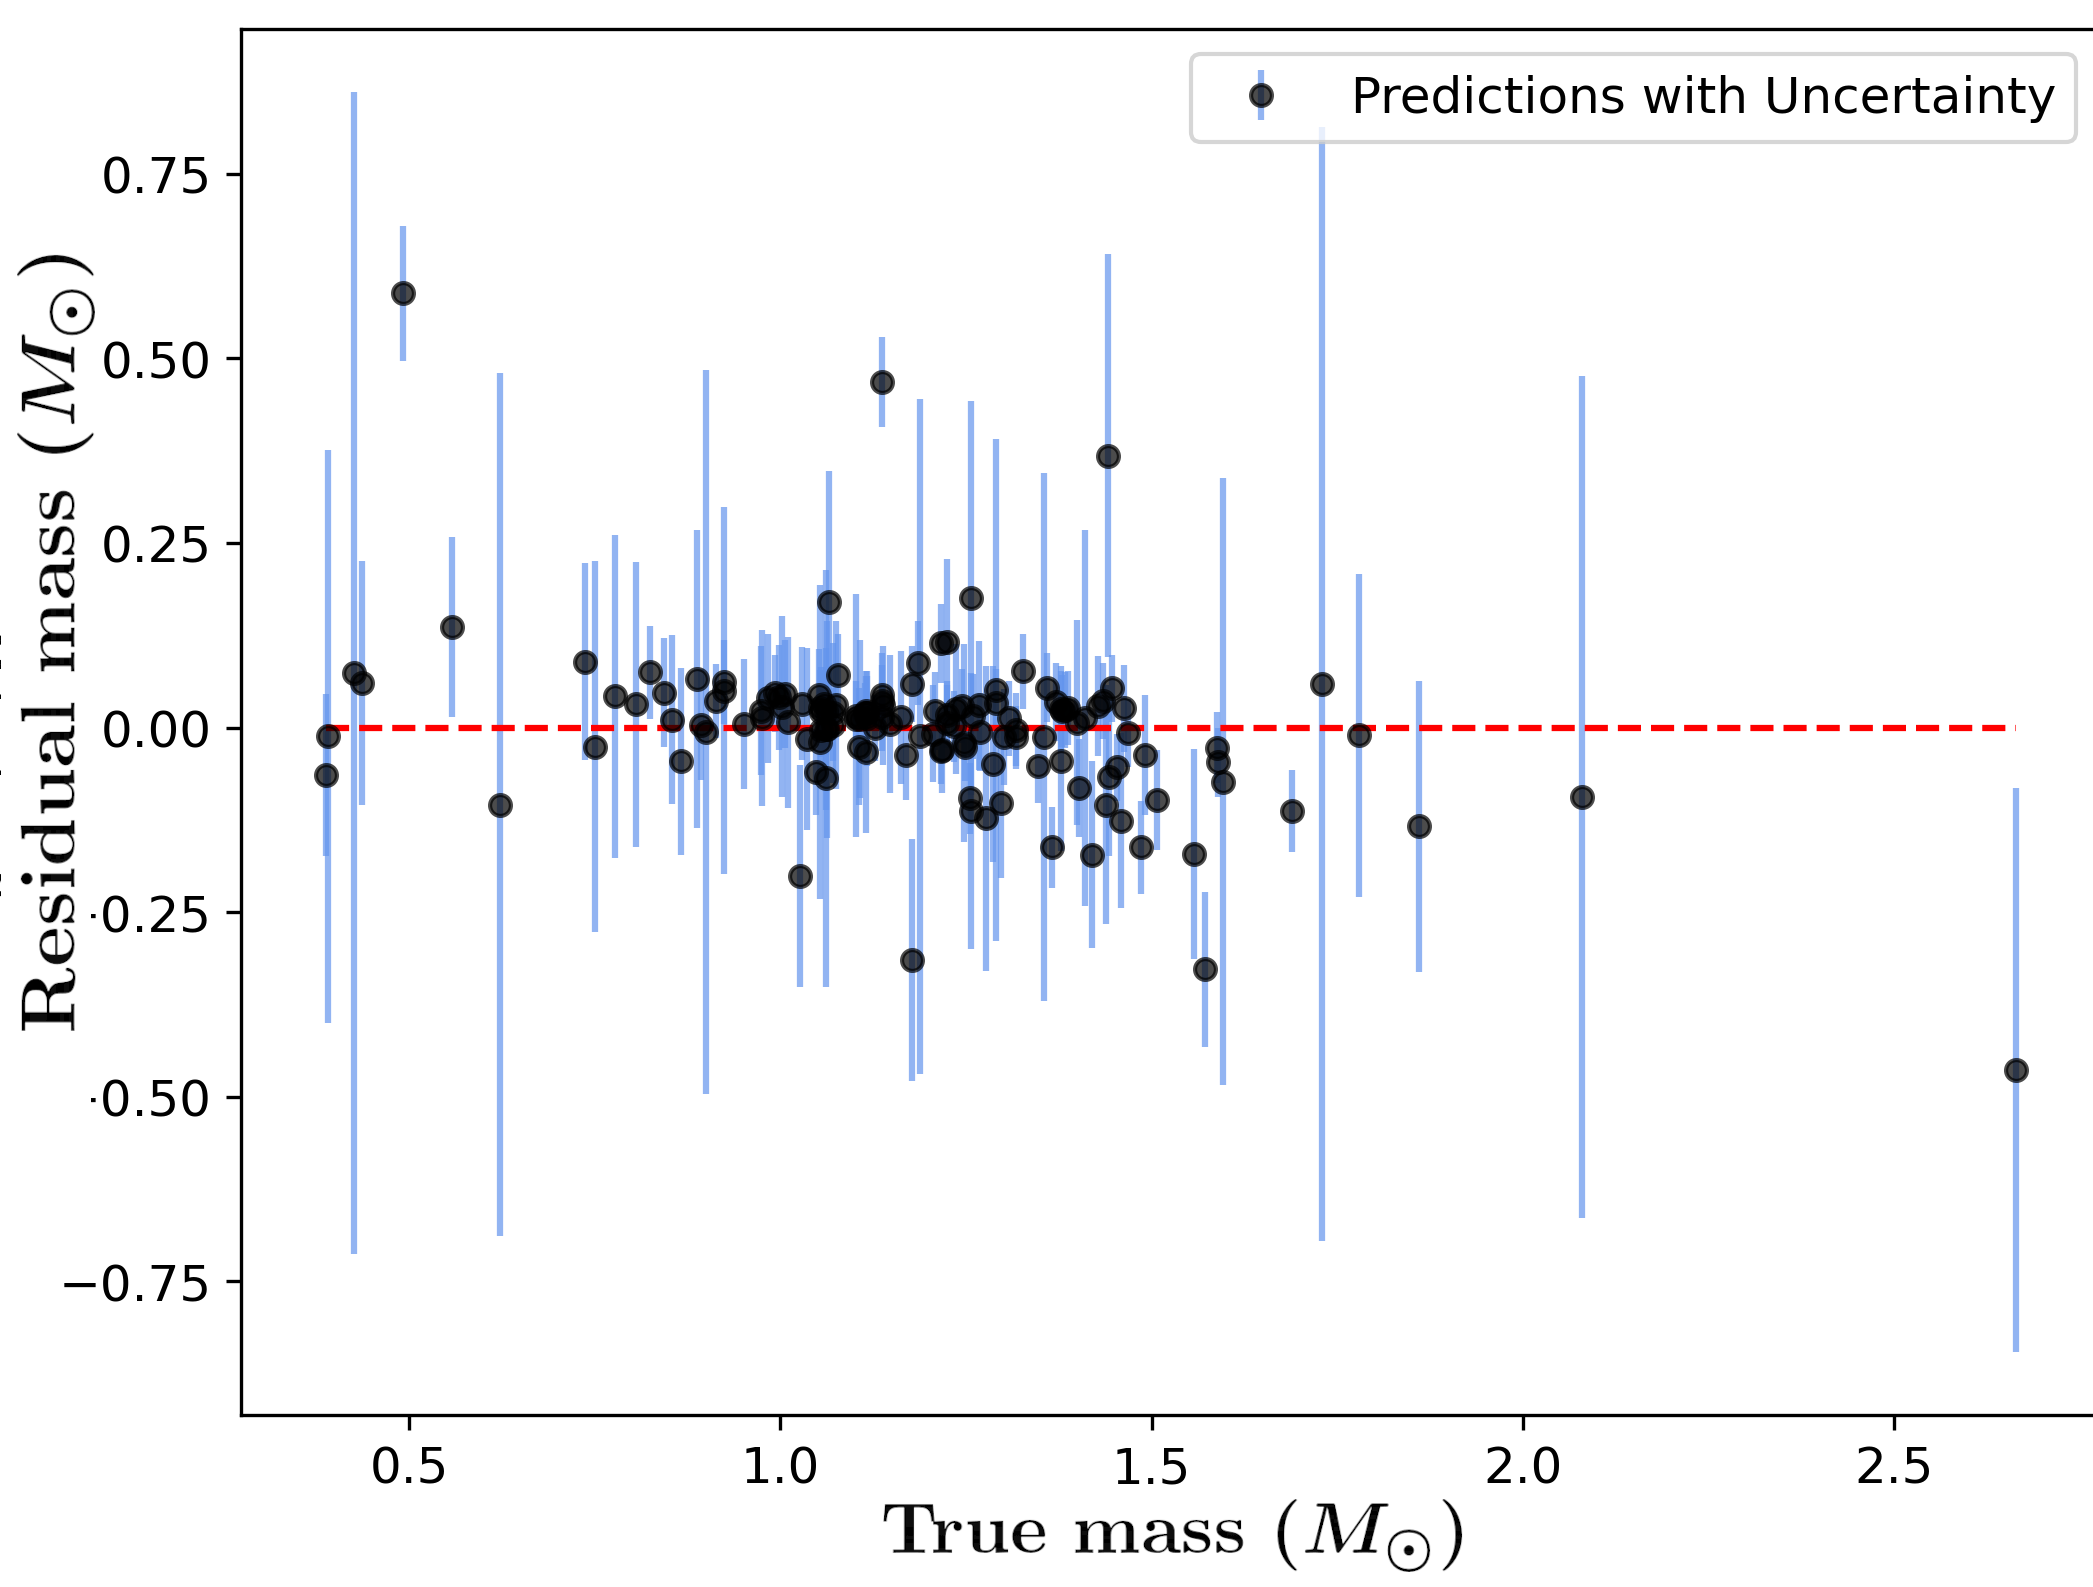
\includegraphics[width=\linewidth]{GP_mass_3param_L_1000_draws_4_chains_80_40_seed_176_filtered_90_residual_no_title_smaller_points_fontplus2.png}
\caption{GP residuals.}
\label{fig:gp_mass_residuals_B}
\end{subfigure}

\vspace{0.4cm}

% Bottom row: BART, BHS
\begin{subfigure}[t]{0.24\textwidth}
\centering
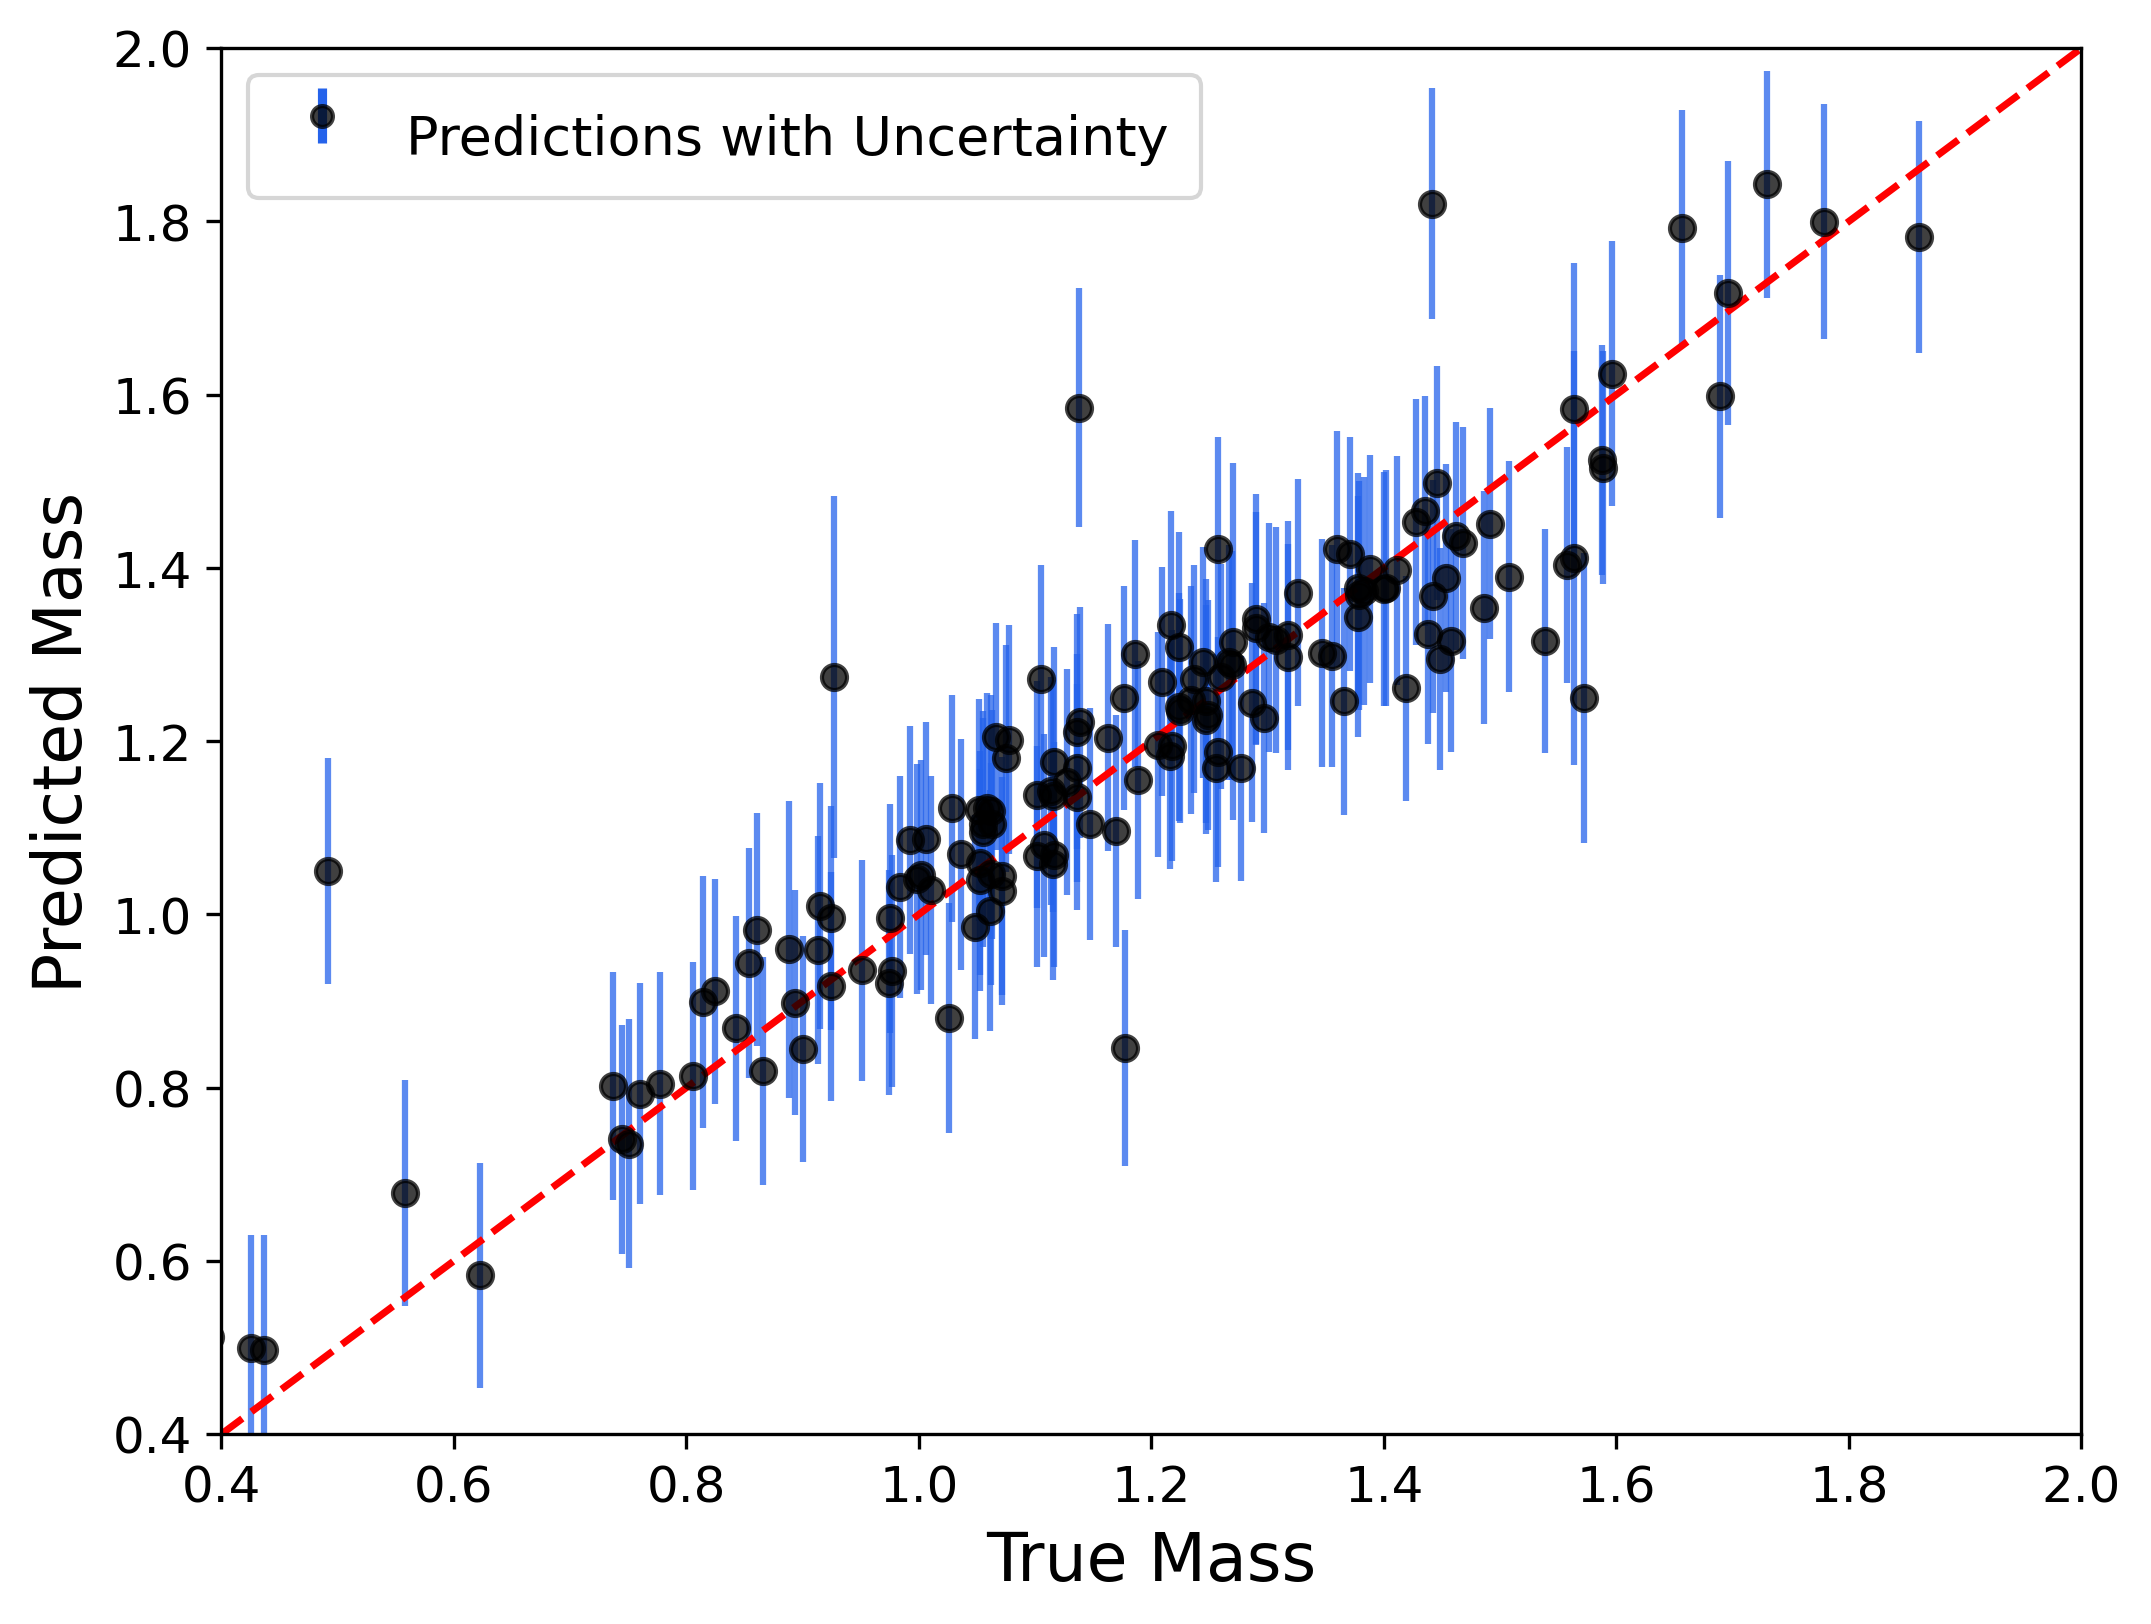
\includegraphics[width=\linewidth]{BART_mass_3param_L_prediction_seed_176_full_prediction_fontminus2_vertical_legend.png}
\caption{BART prediction.}
\label{fig:bart_mass_predictions_B}
\end{subfigure}
\hfill
\begin{subfigure}[t]{0.24\textwidth}
\centering
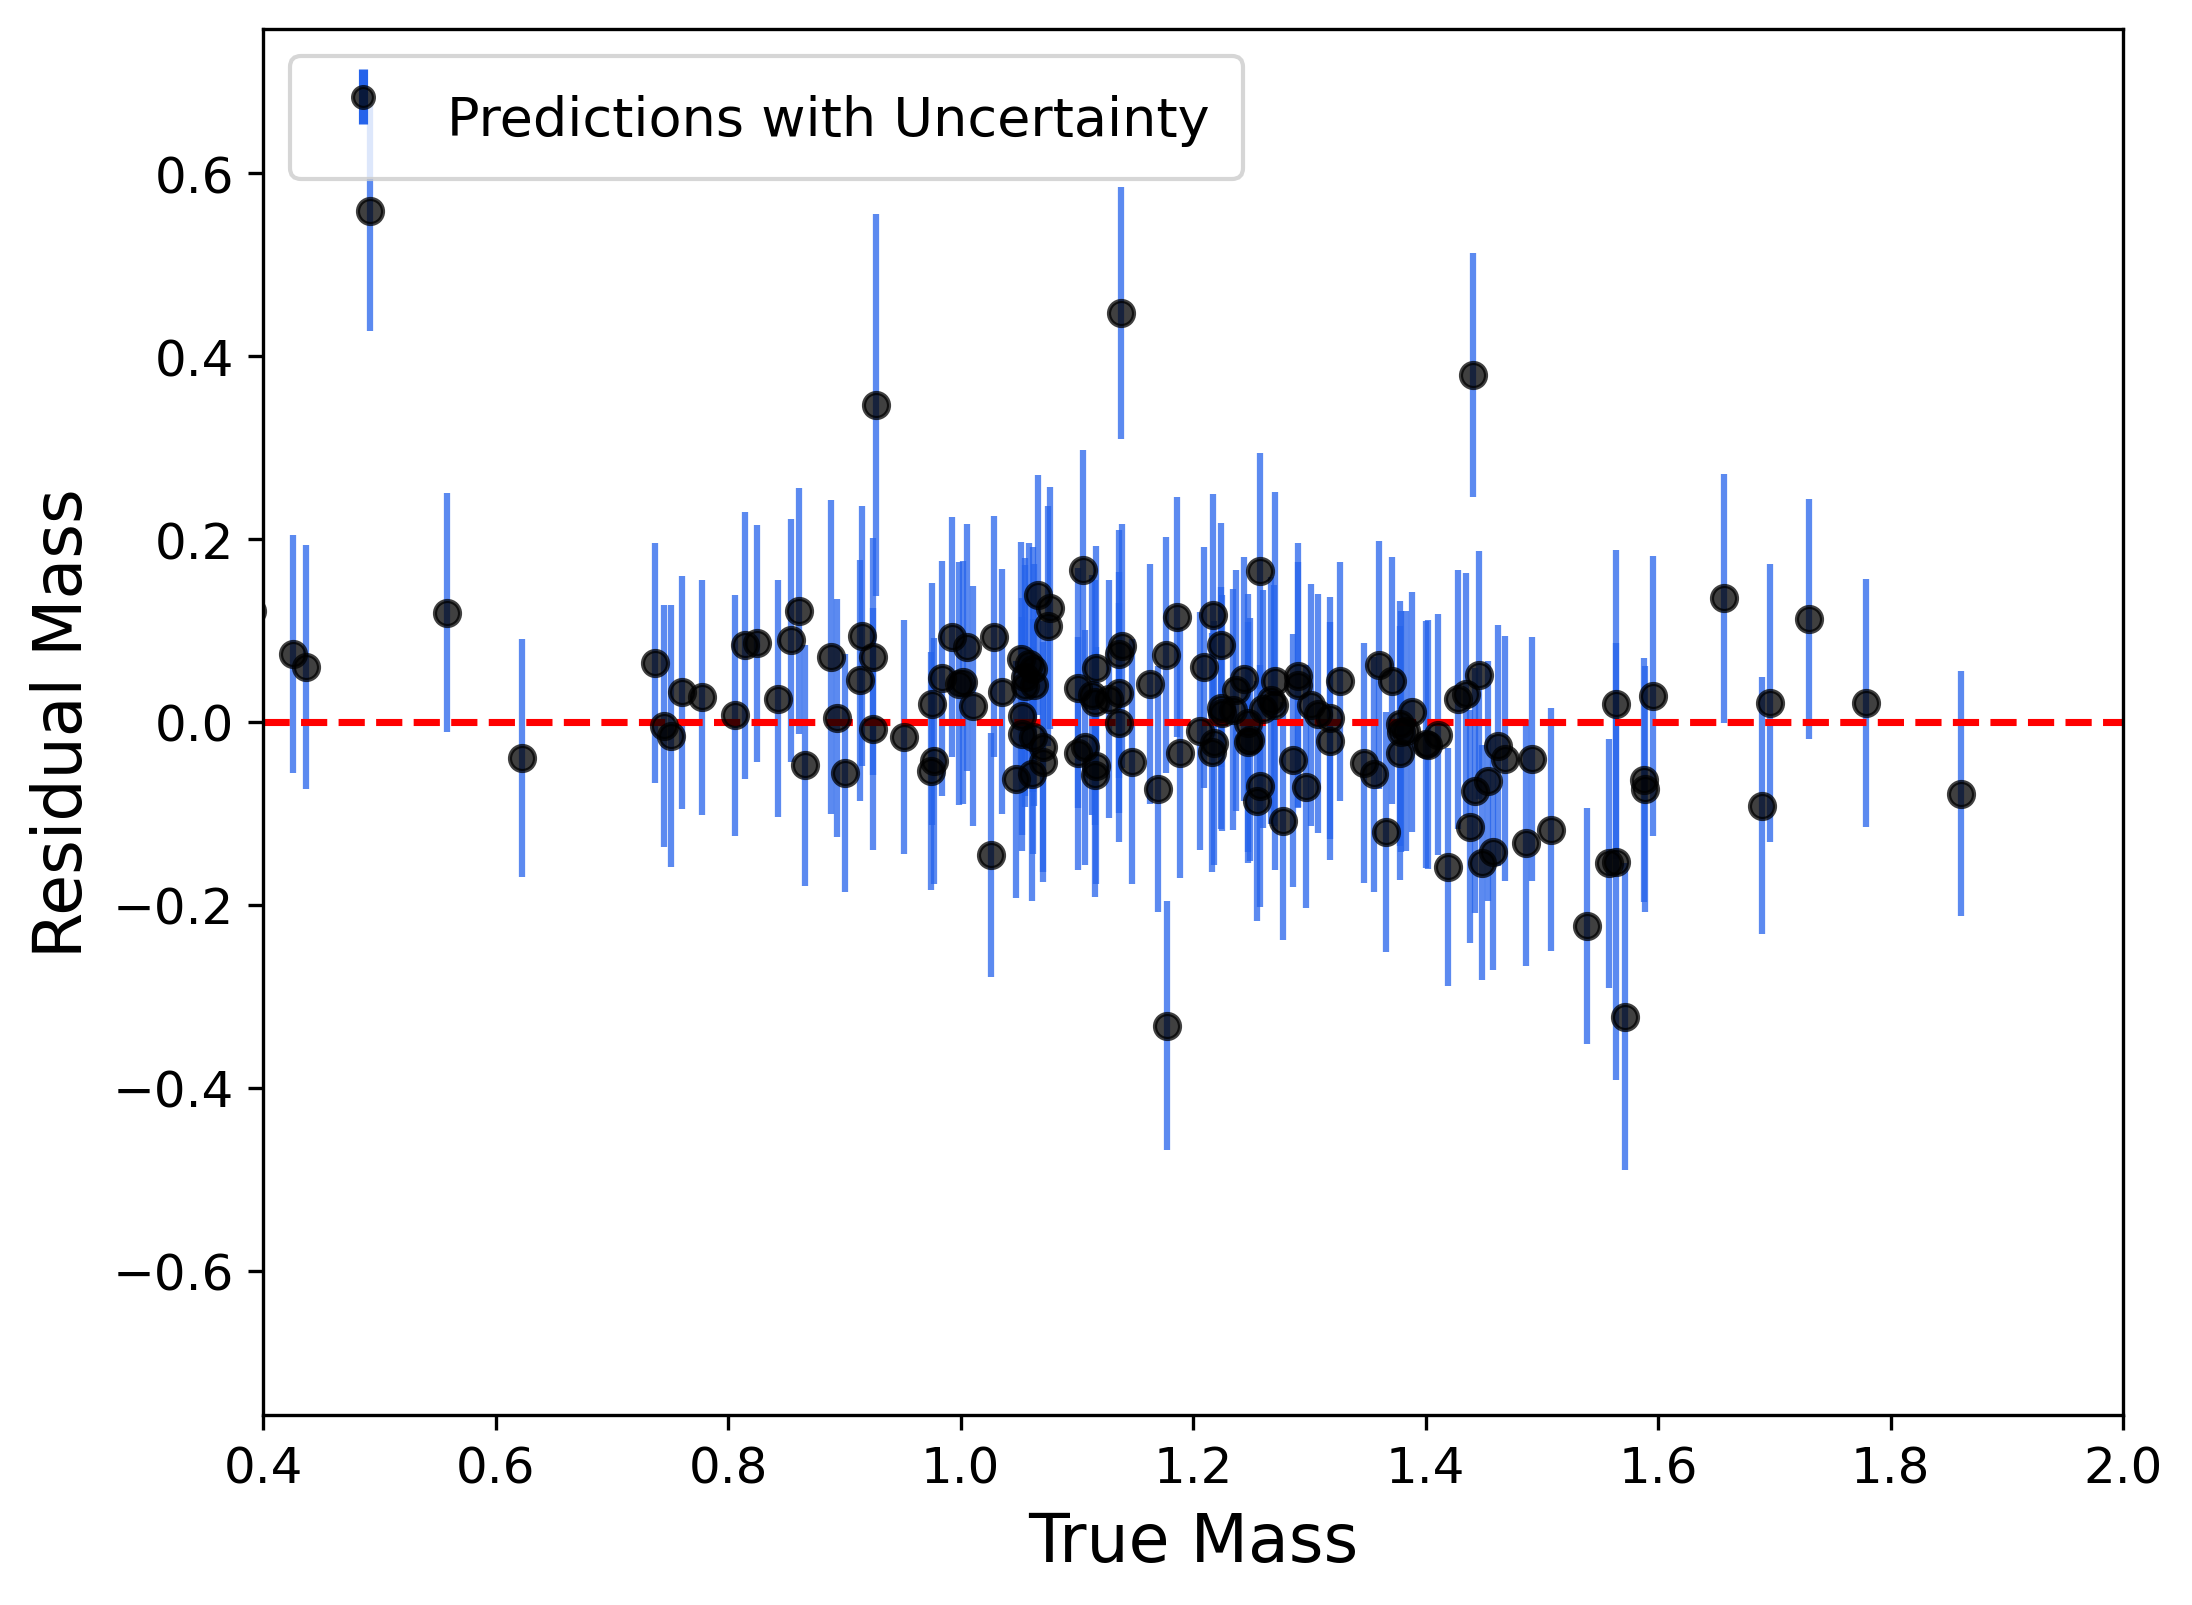
\includegraphics[width=\linewidth]{BART_mass_3param_L_prediction_seed_176_full_residual_fontminus2_vertical_legend.png}
\caption{BART residuals.}
\label{fig:bart_mass_residuals_B}
\end{subfigure}
\hfill
\begin{subfigure}[t]{0.24\textwidth}
\centering
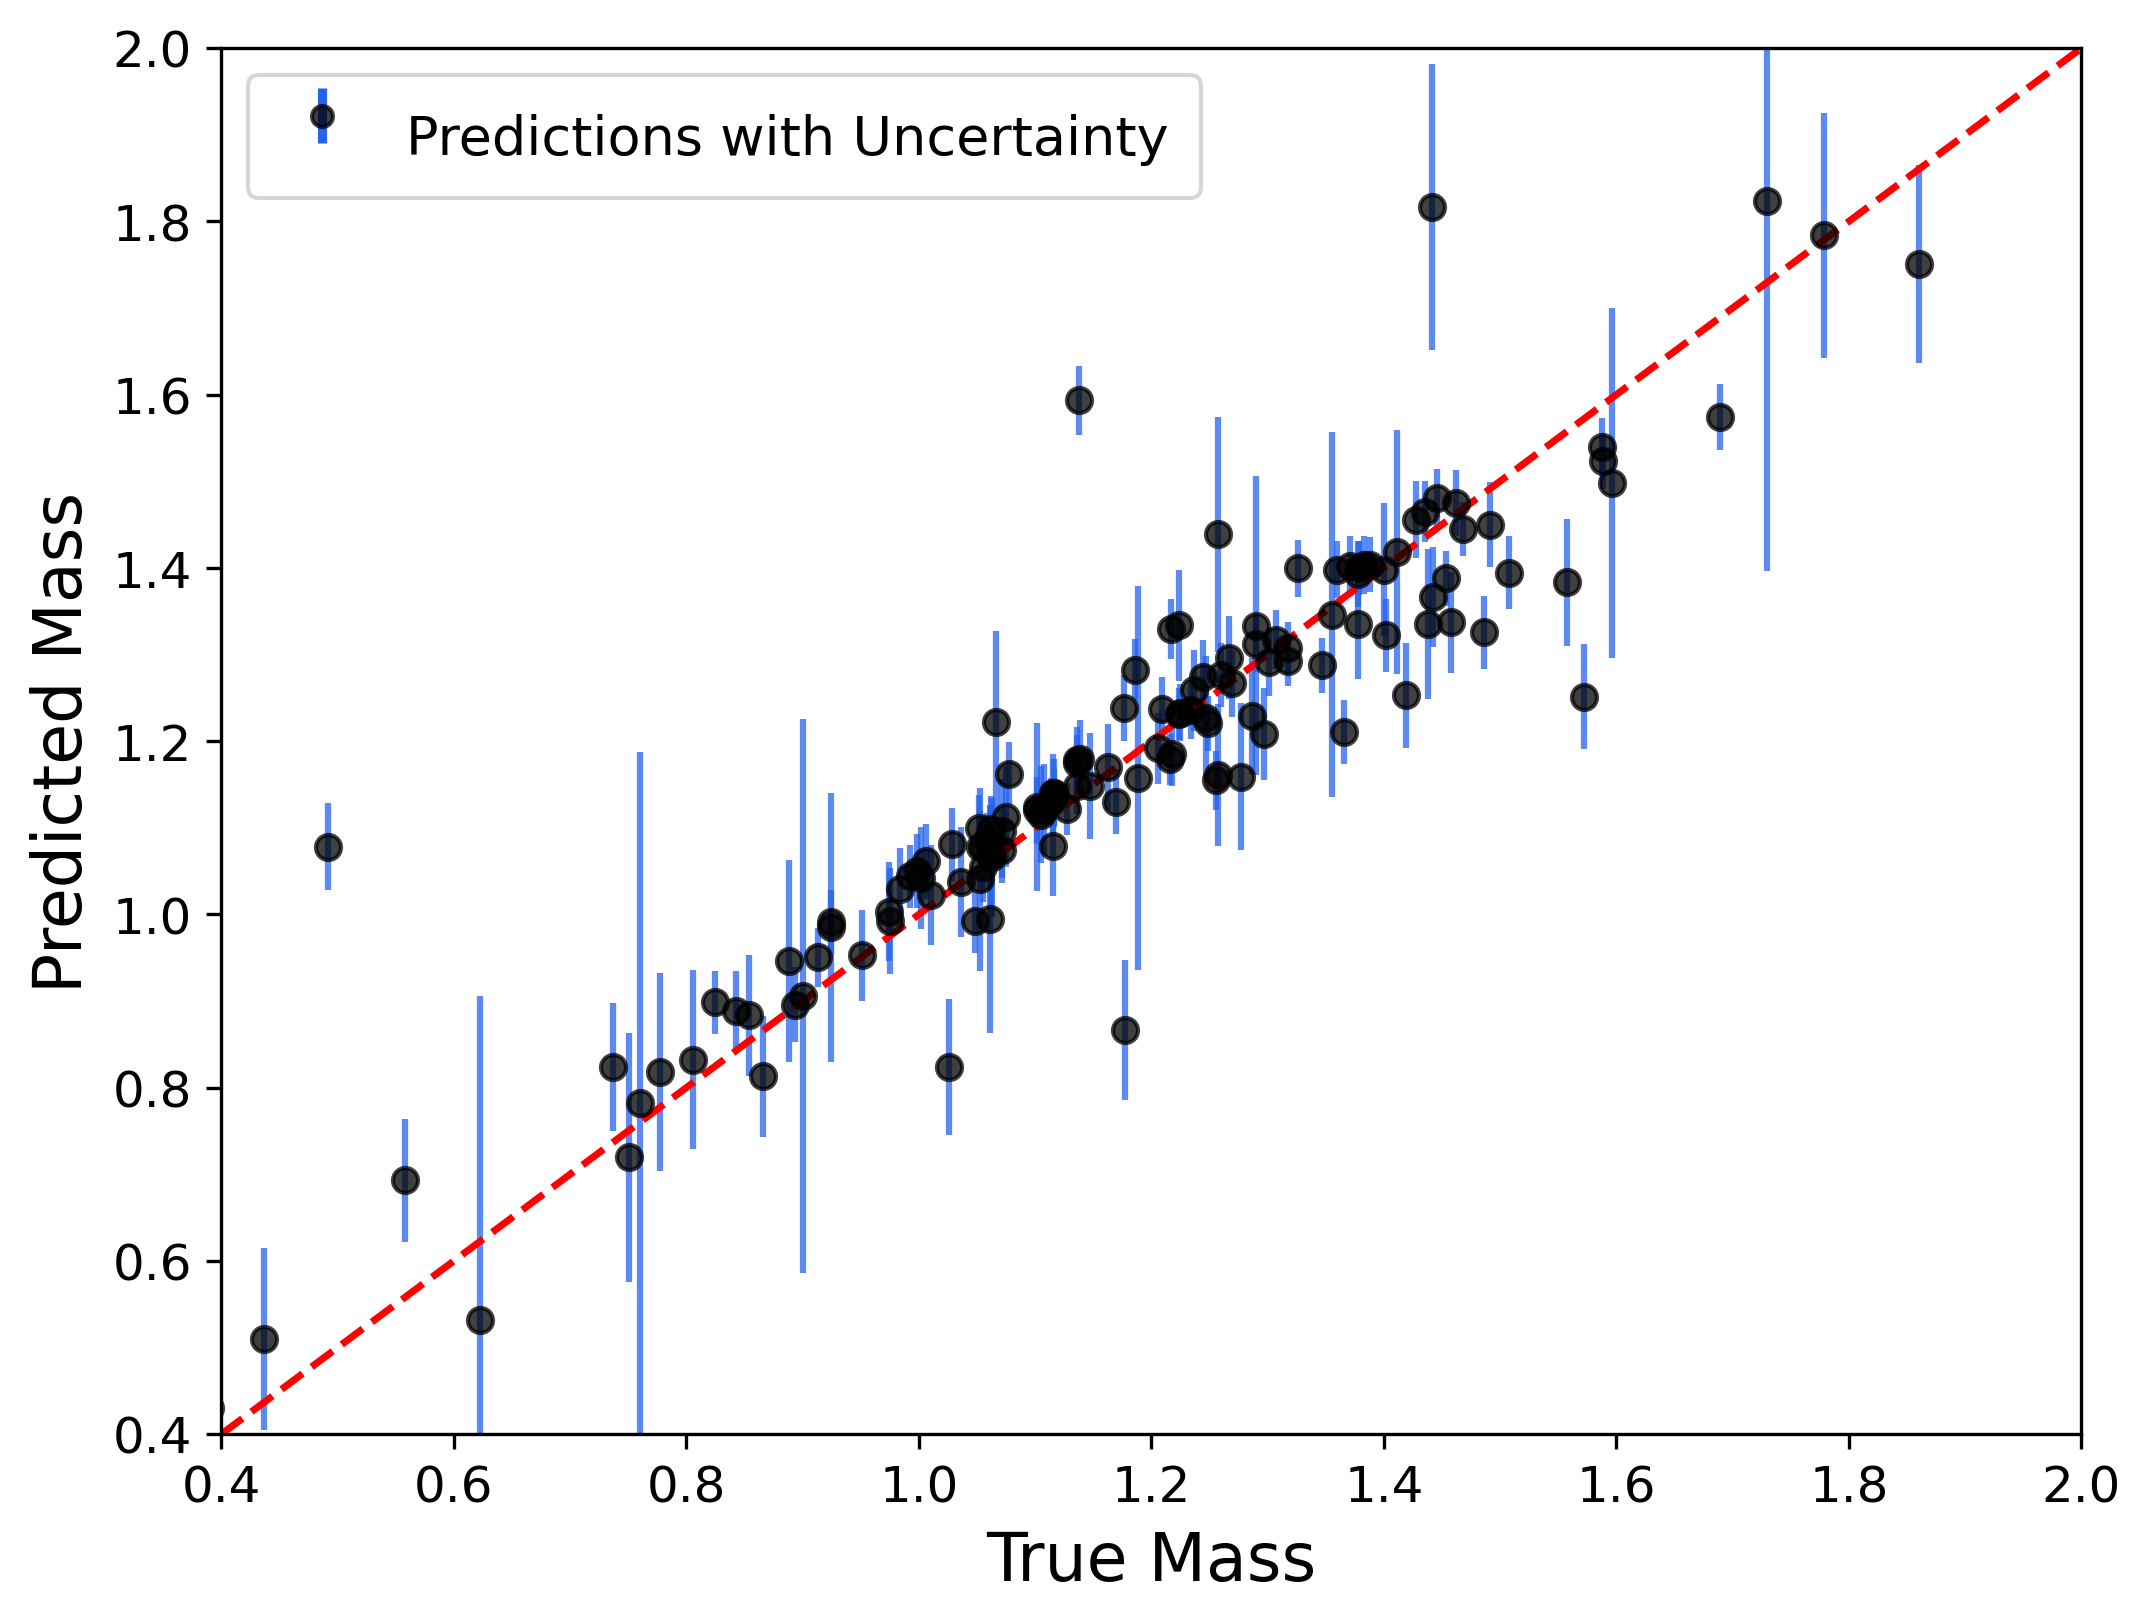
\includegraphics[width=\linewidth]{BHS_mass_3param_L_prediction_seed_176_filtered_90_prediction_fontminus2_vertical_legend.png}
\caption{BHS prediction.}
\label{fig:bhs_mass_predictions_B}
\end{subfigure}
\hfill
\begin{subfigure}[t]{0.24\textwidth}
\centering
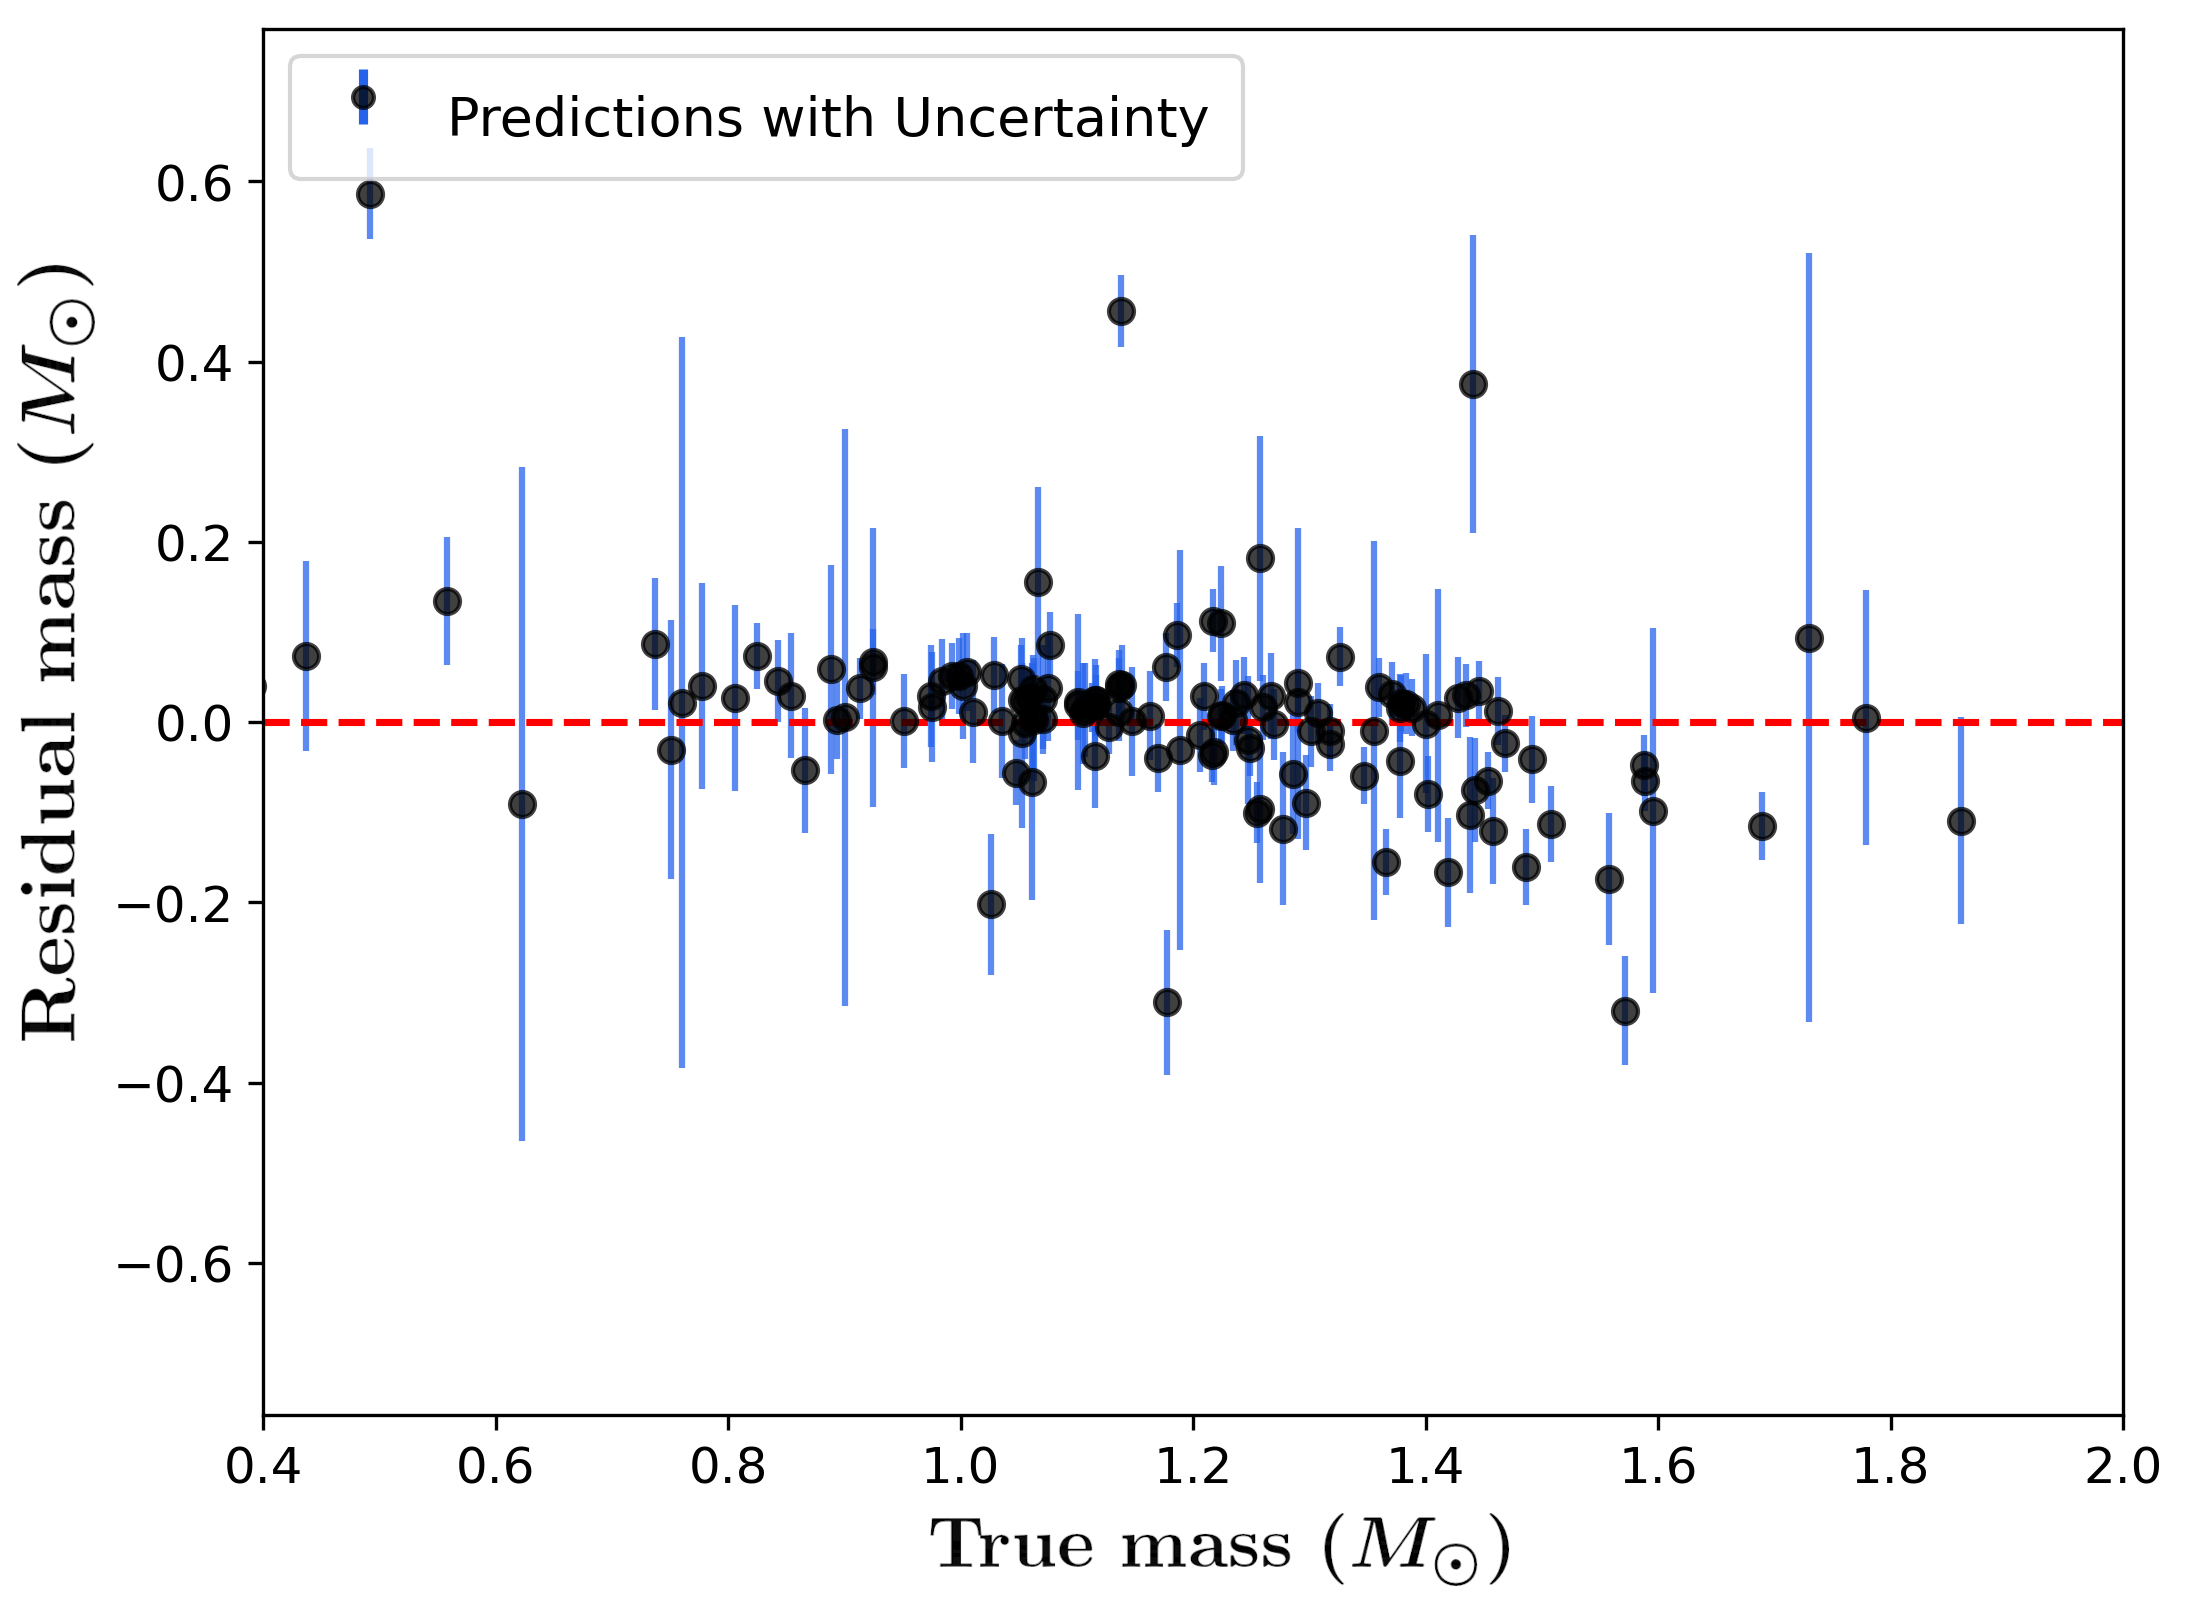
\includegraphics[width=\linewidth]{BHS_mass_3param_L_prediction_seed_176_filtered_90_residual_fontminus2_clear_vertical_legend.png}
\caption{BHS residuals.}
\label{fig:bhs_mass_residuals_B}
\end{subfigure}

\caption{Holdout-test performance of the HBNN, GP, BART and BHS mass models trained with $T_{\mathrm{eff}}$, $L$ and $[\mathrm{Fe}/\mathrm{H}]$. For each model, the prediction panel shows $M_{\mathrm{pred}}$ as a function of $M_{\mathrm{true}}$, while the residual panel shows $M_{\mathrm{pred}}-M_{\mathrm{true}}$ as a function of $M_{\mathrm{true}}$. Vertical error bars represent the predictive uncertainty returned by each model. The GP and BHS panels are restricted to the stars below the 95th percentile of predicted mass uncertainty in order to keep the main population visually readable. The full calibration sample contains $n=767$ stars, with $20\%$ reserved for the holdout test.}
\label{fig:mass_holdout_all_models_B}

\end{figure}

BHS combines the behaviours of the three level-0 models and remains the most stable compromise between residual accuracy and global bias. Since GP performs better away from $1\,M_\odot$ than BART and HBNN, the stacking approach is expected to assign it larger weight in those regions. In the central region, however, BHS can favour the other models when they provide more reliable predictions. Overall, the points remain well concentrated around the 1:1 relation, with no clear systematic trend. Although the BHS MRD is slightly worse than the GP value, this is expected because the stacking model does not simply reproduce the GP predictions, but balances them with the contributions of BART and HBNN. This behaviour is consistent with the evaluation metrics. The large individual predictive uncertainties of the stacking model suggest that it inherits part of the underconfidence already present in BART and GP, a behaviour also observed in the $\rho$-training case.


The mass predictions, including their uncertainties, are then compared with the stellar evolutionary-grid estimates based on PARSEC \citep{bressan2012} and with the linear-relation masses presented by \citet{moya2018}. The differences are analysed through fractional residuals, defined as $(M_1-M_2)/M_2$, where $M_1$ and $M_2$ correspond to the first and second methods indicated in each comparison label in Figure \ref{fig:frac_res_distrib_dataset_b}. The closest agreement is found between the BHS predictions and the grid-model masses: in this case, all residuals remain within approximately $\pm 10\%$. The stacking approach gives systematically higher masses than the grid models, but in a relatively homogeneous way, since both the mean and the median lie close to each other, near a fractional difference of $+2\%$.

When BHS is compared with the \citet{moya2018} linear relations, the behaviour changes, showing a more dispersed distribution with a tail of mass differences up to about $15\%$. The near-zero mean residual should not be interpreted as evidence that the stacking approach and the linear relations are consistently equivalent, but rather as the result of a broader residual distribution in which positive and negative deviations partly cancel. Table \ref{tab:residuals_dataset_b} confirms this interpretation: the mean residual is $-0.38\%$, while the mean absolute residual increases to $3.14\%$, larger than the BHS-grid comparison value of $2.86\%$. The two methods therefore provide different predictions for individual stars, even though their average signed offset is small.

\begin{figure}[H]
\centering
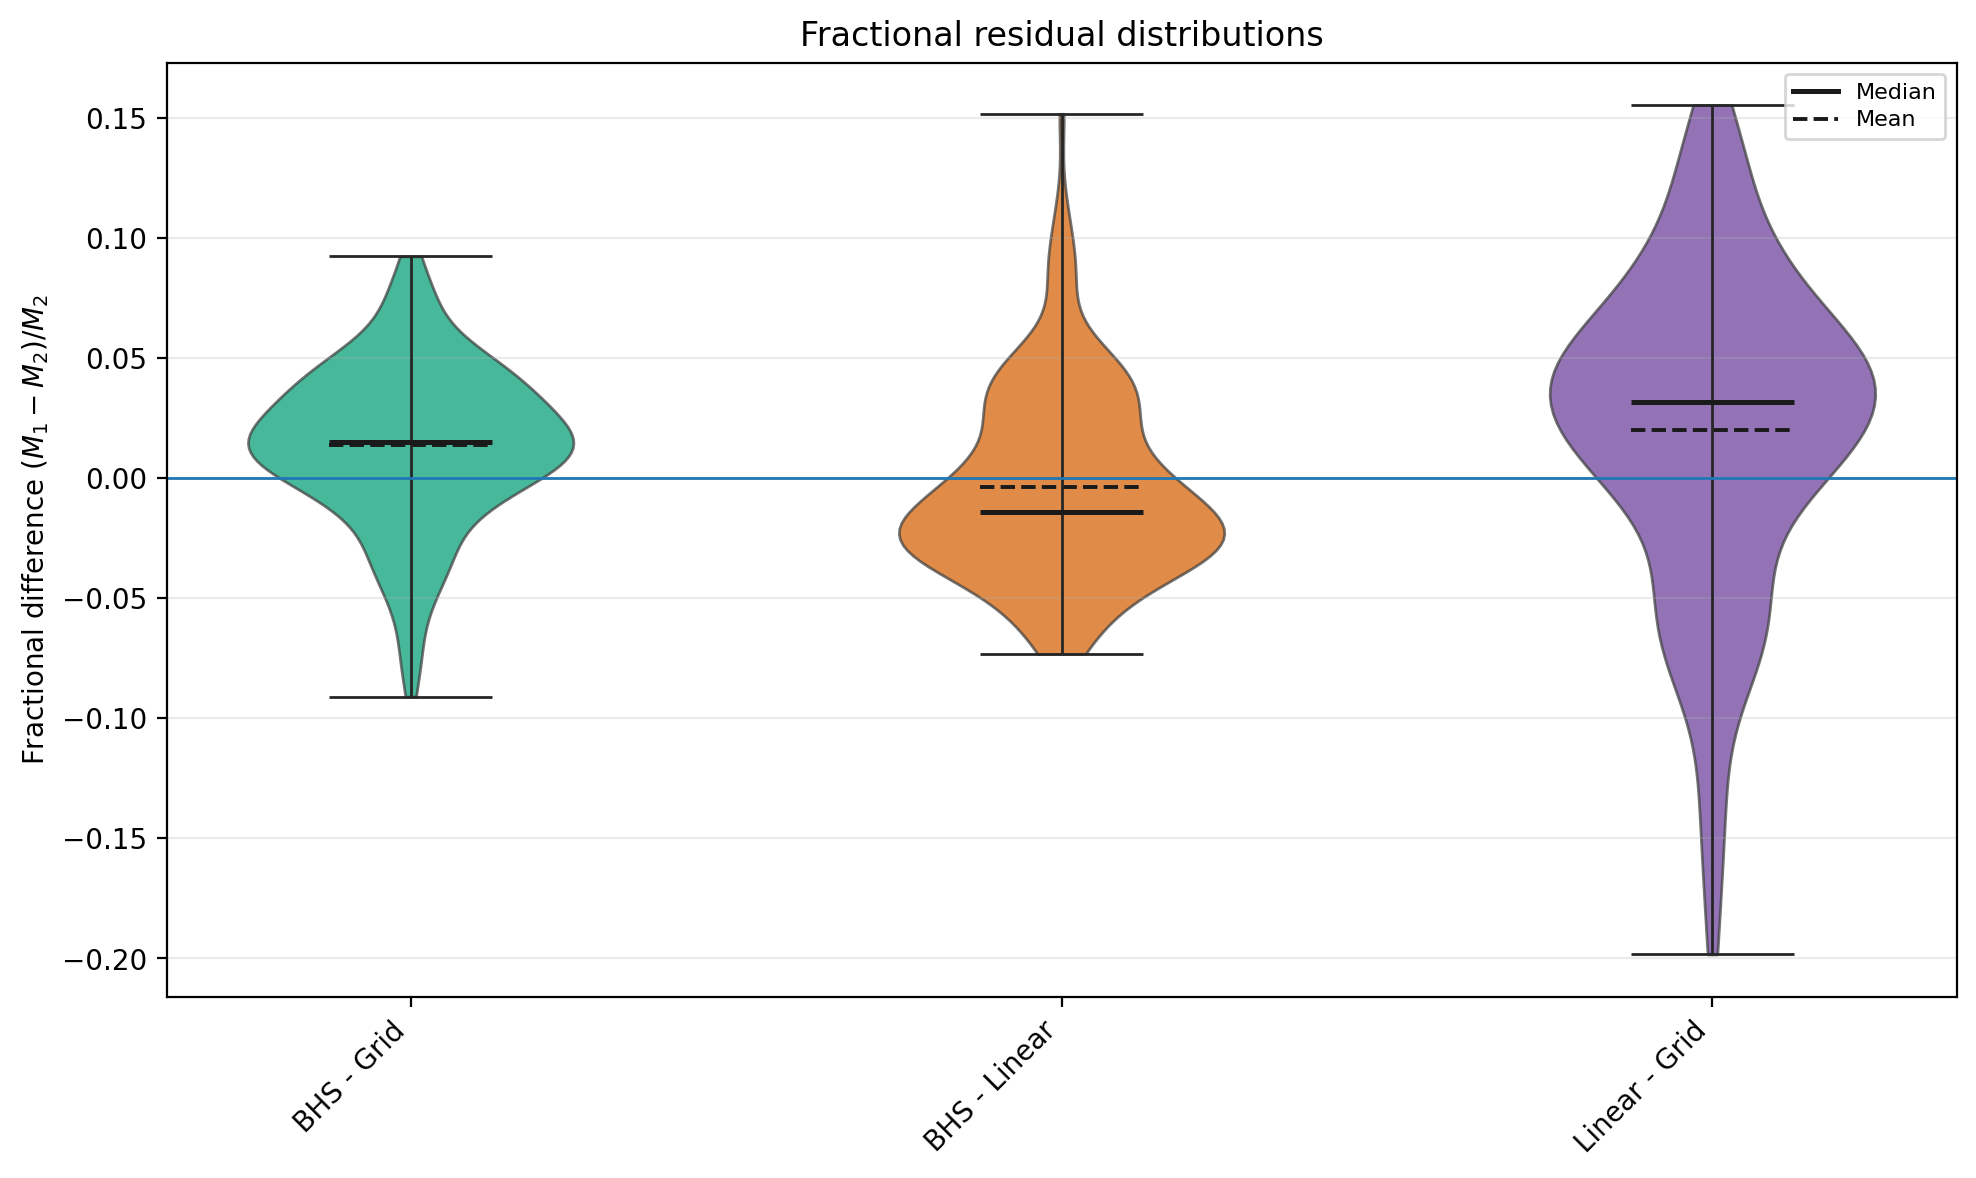
\includegraphics[width=0.8\linewidth]{mass_predictions_seed_819_without_bhs_2022_fractional_residual_distributions.png}
\caption{Distributions of fractional mass residuals for the comparison between the Bayesian Hierarchical Stacking predictions and the two reference mass estimates used for the ARIEL sample. The green distribution compares BHS with the stellar-model grid masses provided by the IA-Porto group, while the orange distribution compares BHS with the linear-relation masses from \citet{moya2018}. The purple distribution shows the direct comparison between the linear-relation and grid masses. The fractional residuals are defined as $(M_1-M_2)/M_2$, following the order of the two methods shown on the horizontal axis. The sample contains $n=184$ stars.}
\label{fig:frac_res_distrib_dataset_b}
\end{figure}

The two reference models do not produce equivalent predictions either. Figure \ref{fig:frac_res_distrib_dataset_b} and Table \ref{tab:residuals_dataset_b} show that the linear-relation and grid masses differ more strongly from each other than BHS differs from either of them, with a MARD above $5\%$ and a broad residual distribution that includes a tail of large negative residuals extending almost to $-20\%$. This tail is consistent with the one observed in the BHS-linear comparison, suggesting that the linear relations produce comparatively low masses for a small number of stars.

\begin{table}[H]
\centering
\caption{Mass-comparison metrics for the ARIEL sample using the same fractional-residual convention as in Figure \ref{fig:frac_res_distrib_dataset_b}.}
\begin{tabular}{lccc}
\hline\hline
Metric & BHS - Grid & BHS - Linear & Linear - Grid \\
\hline
MAE ($M_\odot$) & $0.031$ & $0.035$ & $0.061$ \\
MARD [\%] & $2.86$ & $3.14$ & $5.60$ \\
MRD [\%] & $1.39$ & $-0.38$ & $2.01$ \\
\hline
\end{tabular}
\label{tab:residuals_dataset_b}
\end{table}

\subsection{Oblateness and mass predictions of eclipsing binaries} \label{sec:dataset_C}
As explained in Section \ref{subsec:dataset_a}, one of the aims of this work is to predict the masses of FGK-type components in eclipsing-binary systems, so that information can then be inferred for their difficult-to-study M-type companions. Eclipsing binaries therefore provide one of the most useful routes for obtaining information about these objects, but it must be assessed whether the information inferred from stars in eclipsing-binary systems can be extrapolated to isolated stars of similar type.

Eclipsing-binary components are not completely independent objects. Their mutual gravitational interaction can modify their morphology through tidal forces, preventing them from remaining perfectly spherical. This distortion can be quantified through the oblateness parameter $o$, given by Equation (43) of \citet{chandrasekhar1933double}, which classifies stars from perfectly spherical ($o=0$) to highly oblate ($o \sim 1$):

\begin{equation}
o = 0.6446 \cdot \left(1 + 4\frac{m}{m_\star}\right) \cdot \left(\frac{R_\star}{a}\right)^3,
\label{eq:oblateness}
\end{equation}
where $R_\star$ and $m_\star$ are the radius and mass of the star whose oblateness is being computed, $m$ is the mass of its companion, and $a$ is the orbital semi-major axis.

To test whether this tidal distortion affects the mass predictions, the models are trained on asteroseismic stars, which are treated here as the single-star reference sample. Predictions are then obtained for the eclipsing-binary components available in the catalogue. The predicted masses are compared with the reference masses of the eclipsing-binary stars, and the resulting residuals are analysed as a function of oblateness. This follows the general approach of \citet{maxted2023benchmark}, where eclipsing binaries are used to evaluate how well single-star relations can be transferred to binary systems.

\subsubsection*{Results: holdout test}
The models were trained using the asteroseismic stars from the dataset in Table \ref{MS_catalog_database_D}. Since the goal in this section is to obtain accurate mass predictions before analysing the residual dependence on oblateness, four input features were used, following the recommendation of \citet{moya2022}: $T_{\mathrm{eff}}$, $\log g$, $L$ and $[\mathrm{Fe}/\mathrm{H}]$. This subset contains 420 stars, of which 84 were retained as the holdout set. There are therefore two competing effects on the predictive performance of the models. On the one hand, the models now use four input features instead of three, which should improve the precision of the predictions. On the other hand, the available sample is reduced from the original 767 stars to 420 stars. 

\begin{table}[H]
    \centering
    \caption{Comparison of the residual metrics obtained by the mass-prediction models on the holdout set. The models were trained with $T_{\mathrm{eff}}$, $\log g$, $L$ and $[\mathrm{Fe}/\mathrm{H}]$ as input features, and stellar mass as the target.}
    \label{tab:dataset_D_model_mard_mrd}
    \begin{tabular}{lcccc}
        \hline\hline
        Metric & BART & GP & HBNN & BHS \\
        \hline
        MAE ($M_\odot$) & $0.052$ & $0.042$ & $0.045$ & $0.043$ \\
        MARD [\%] & $4.50$ & $3.84$ & $3.98$ & $3.85$ \\
        MRD [\%]  & $-0.99$ & $-0.69$ & $-0.61$ & $-0.65$ \\
        \hline
    \end{tabular}
\end{table}

The predictions and residuals behave similarly to those discussed in Figure \ref{fig:mass_holdout_all_models}. The characteristic GP behaviour, with a small number of objects showing extremely large predictive uncertainties, is still present, reinforcing the interpretation that the effect is mainly related to the model and its uncertainty treatment, rather than to a fixed set of problematic stars. For HBNN and BART, the systematic behaviour away from $M=1\,M_\odot$ is observed and appears slightly amplified, as seen in Table \ref{tab:dataset_D_model_mard_mrd}. This indicates that, when the models are trained only with asteroseismic stars, the predictions develop a stronger signed bias. However, with $\log g$ included, the resulting metrics have lower values than those of Section \ref{subsec:dataset_b} (Table \ref{tab:dataset_b_mard_mrd}), consistently with the results of \citet{moya2022}.

The stronger signed bias is expected, since the training sample is now less heterogeneous. As shown in Figure \ref{fig:HRdiagram}, the asteroseismic stars are concentrated in a relatively narrow mass range, approximately between $0.8\,M_\odot$ and $1.5\,M_\odot$. This makes the predictions more robust within this specific region of the mass spectrum. Since the holdout test is evaluated against asteroseismic stars from the same population, which mostly occupy the same region of the HR diagram, MARD consequently decreases. However, the predictive performance is expected to be less reliable for stars outside this range, where systematic trends are reflected in the larger absolute MRD values.

Regarding the stacking model, BHS yields the best or nearly best predictions across the evaluated metrics. Although HBNN has a slightly lower MRD, this may reflect the cancellation of systematic overpredictions and underpredictions, as discussed in previous sections. BHS instead provides a more balanced compromise: its MARD is almost identical to that of GP, and its absolute MRD remains well below $1\%$.

\subsubsection*{Results: oblateness}
The effect of binary interaction was studied by predicting the masses of the stars in the original dataset that belong to eclipsing-binary systems. From this group, only systems with an available orbital semi-major axis $a$ could be used, since this parameter is required to compute the oblateness. As explained in Section \ref{sec:cleaning}, this leaves 295 stars with available oblateness estimates before applying the final selection cuts. Once $o$ was computed, the models trained on the asteroseismic stars were applied to these eclipsing-binary components, and the resulting mass residuals were analysed as a function of oblateness.

To avoid interpreting extrapolation effects as physical binary effects, the eclipsing-binary sample was restricted to stars well covered by the asteroseismic training set. First, only stars with $0.950\,M_\odot < M < 1.500\,M_\odot$ were retained, corresponding approximately to the 5th and 95th mass percentiles of the asteroseismic sample. In addition, the final sample was restricted to the input-parameter domain $5500 < T_{\mathrm{eff}} < 6800\,\mathrm{K}$, $3.750 < \log g < 4.450$, $1.000 < L/L_\odot < 11.000$ and $-0.500 < [\mathrm{Fe}/\mathrm{H}] < 0.270$, corresponding to the 2nd and 98th percentiles of the asteroseismic training distribution. The final eclipsing-binary sample contains $n=85$ stars. This conservative selection reduces the number of systems, but makes the comparison more reliable, since the remaining stars lie inside the region of parameter space where the model is expected to have predictive validity.

The analysis was carried out using $\log o$, since the oblateness values span several orders of magnitude, as Figure \ref{fig:dataset_D_o} shows. Globally, the signed residuals show no strong systematic tendency towards either overprediction or underprediction. Pearson and Spearman tests support this interpretation, since both yield correlation coefficients close to zero. The mean fractional residual is $\overline{\delta M}=-0.85\%$, while the standard deviation reaches $10.43\%$, driven partly by a small number of large residuals and the reduced number of training stars. Therefore, the model is approximately unbiased on the selected eclipsing-binary sample, but the scatter is not negligible.

\begin{figure}[H]
\centering

\begin{subfigure}[t]{0.49\textwidth}
    \centering
    
\includegraphics[width=\textwidth]{10_bins_02_fractional_residual_vs_log10_oblateness.png}
    \caption{Signed fractional mass residuals.}
    \label{fig:dataset_D_o_residuals}
\end{subfigure}
\hfill
    \begin{subfigure}[t]{0.49\textwidth}
    \centering
    
\includegraphics[width=\textwidth]{10_bins_02c_abs_fractional_residual_vs_log10_oblateness.png}
    \caption{Absolute fractional mass residuals.}
    \label{fig:dataset_D_o_residuals_abs}
\end{subfigure}
\caption{Dependence of the BHS mass residuals on stellar oblateness $o$, as defined in Equation \ref{eq:oblateness}, for the selected eclipsing-binary sample. The model uses $T_{\mathrm{eff}}$, $L$, $\log g$ and $[\mathrm{Fe}/\mathrm{H}]$ as input parameters. Grey points correspond to individual eclipsing-binary components, and the blue and red squares show binned means and medians with $1\sigma$ scatter. The sample contains $n=85$ stars.}
\label{fig:dataset_D_o}

\end{figure}

Figure \ref{fig:dataset_D_o_residuals_abs} shows that the dispersion of the residuals increases with $o$. In the signed residual analysis, the standard deviation of $\delta M$ rises from values of a few percent at low oblateness to much larger values in the most deformed systems: $1.06\%$, $2.65\%$, $6.50\%$, $9.89\%$, $6.23\%$, $7.57\%$, $9.77\%$, $13.87\%$ and $22.74\%$. The overall behaviour is consistent with a degradation of precision at larger oblateness. If a residual scatter of about $10\%$ is adopted as a practical tolerance for acceptable predictions, the transition occurs around $\log o \simeq -2$, corresponding to $o \simeq 0.01$. The same trend is visible in the absolute fractional residuals: most bins below this value remain below about $7\%$, whereas higher-oblateness bins reach approximately $15\%$. Therefore, the main effect of oblateness is not a clear change in the sign of the residuals, but an increase in their spread.

This distinction is important. The results do not indicate a systematic loss of accuracy, since the average residual remains close to zero. Instead, they indicate a loss of precision: as the stars become more oblate, the model predictions become more dispersed around the true eclipsing-binary masses. In this sample, $o \simeq 0.01$ provides an approximate practical limit beyond which the predictions begin to deviate more strongly from the behaviour expected for the approximately isolated stellar evolution represented by the asteroseismic training sample. Nevertheless, this interpretation should remain cautious, because the number of stars is limited and the inferred threshold depends on the adopted tolerance and the chosen bin edges.

Since Sections \ref{subsec:dataset_a} and \ref{subsec:dataset_b} showed that stellar mass has a strong effect on the predictions, it is necessary to check whether the observed increase in scatter could instead be driven by $M$. Figure \ref{fig:dataset_D_mass} shows that this is not the case: the residual dispersion does not display a clear dependence on stellar mass. If anything, the residual panel in Figure \ref{fig:dataset_D_mass_residuals} shows a slight tendency for the models to pull predictions towards values close to $1.25\,M_\odot$. This behaviour was already discussed in detail and is not associated with an increase in prediction scatter; the precision loss appears to be mass-independent. 

The mass-coloured residual panel in Figure \ref{fig:dataset_D_o_residuals_mass_colored} adds the true stellar mass as a colour scale. The points scatter around zero, and many error bars cross the zero-residual line. At the same time, the increase in dispersion at larger oblateness remains visible and not associated with increasing $M_{\mathrm{true}}$, showing that the effect is not confined to a single mass interval.

\begin{figure}[H]
\centering

\begin{subfigure}[t]{0.31\textwidth}
    \centering
    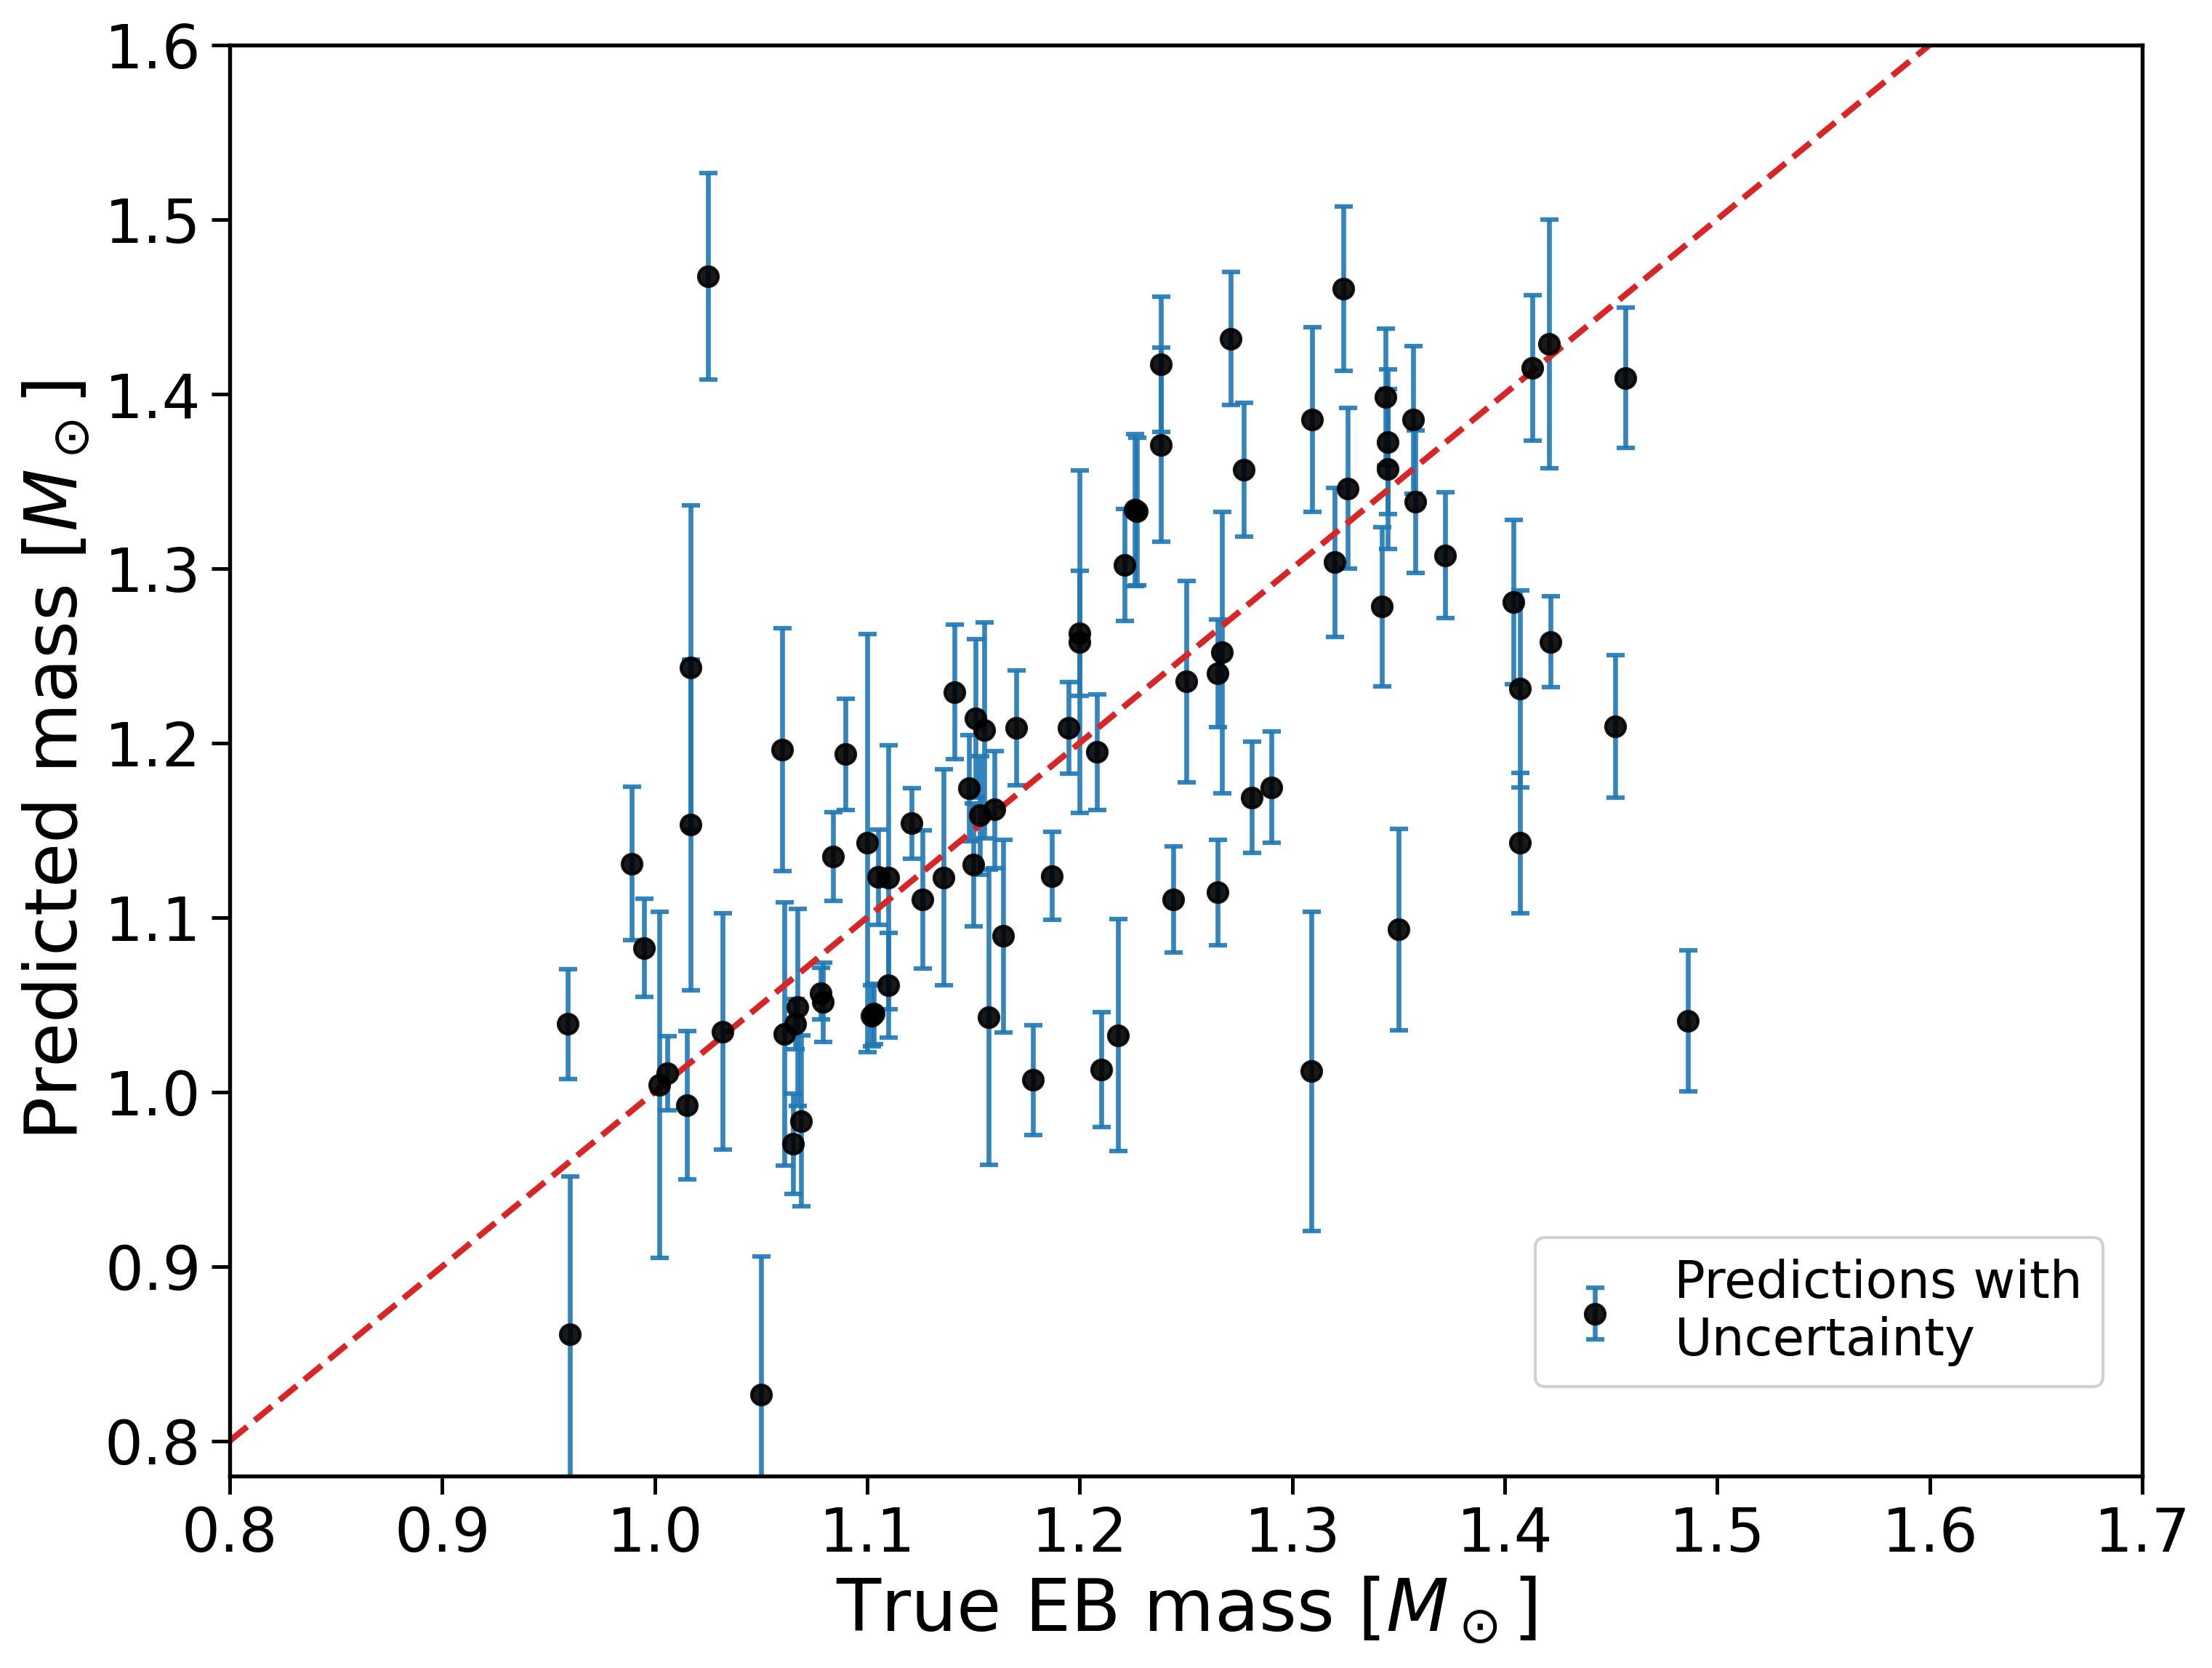
\includegraphics[width=\linewidth]{04_predicted_vs_true_EB_masses.png}
    \caption{Predicted masses.}
    \label{fig:dataset_D_mass_predictions}
\end{subfigure}
\hfill
\begin{subfigure}[t]{0.31\textwidth}
    \centering
    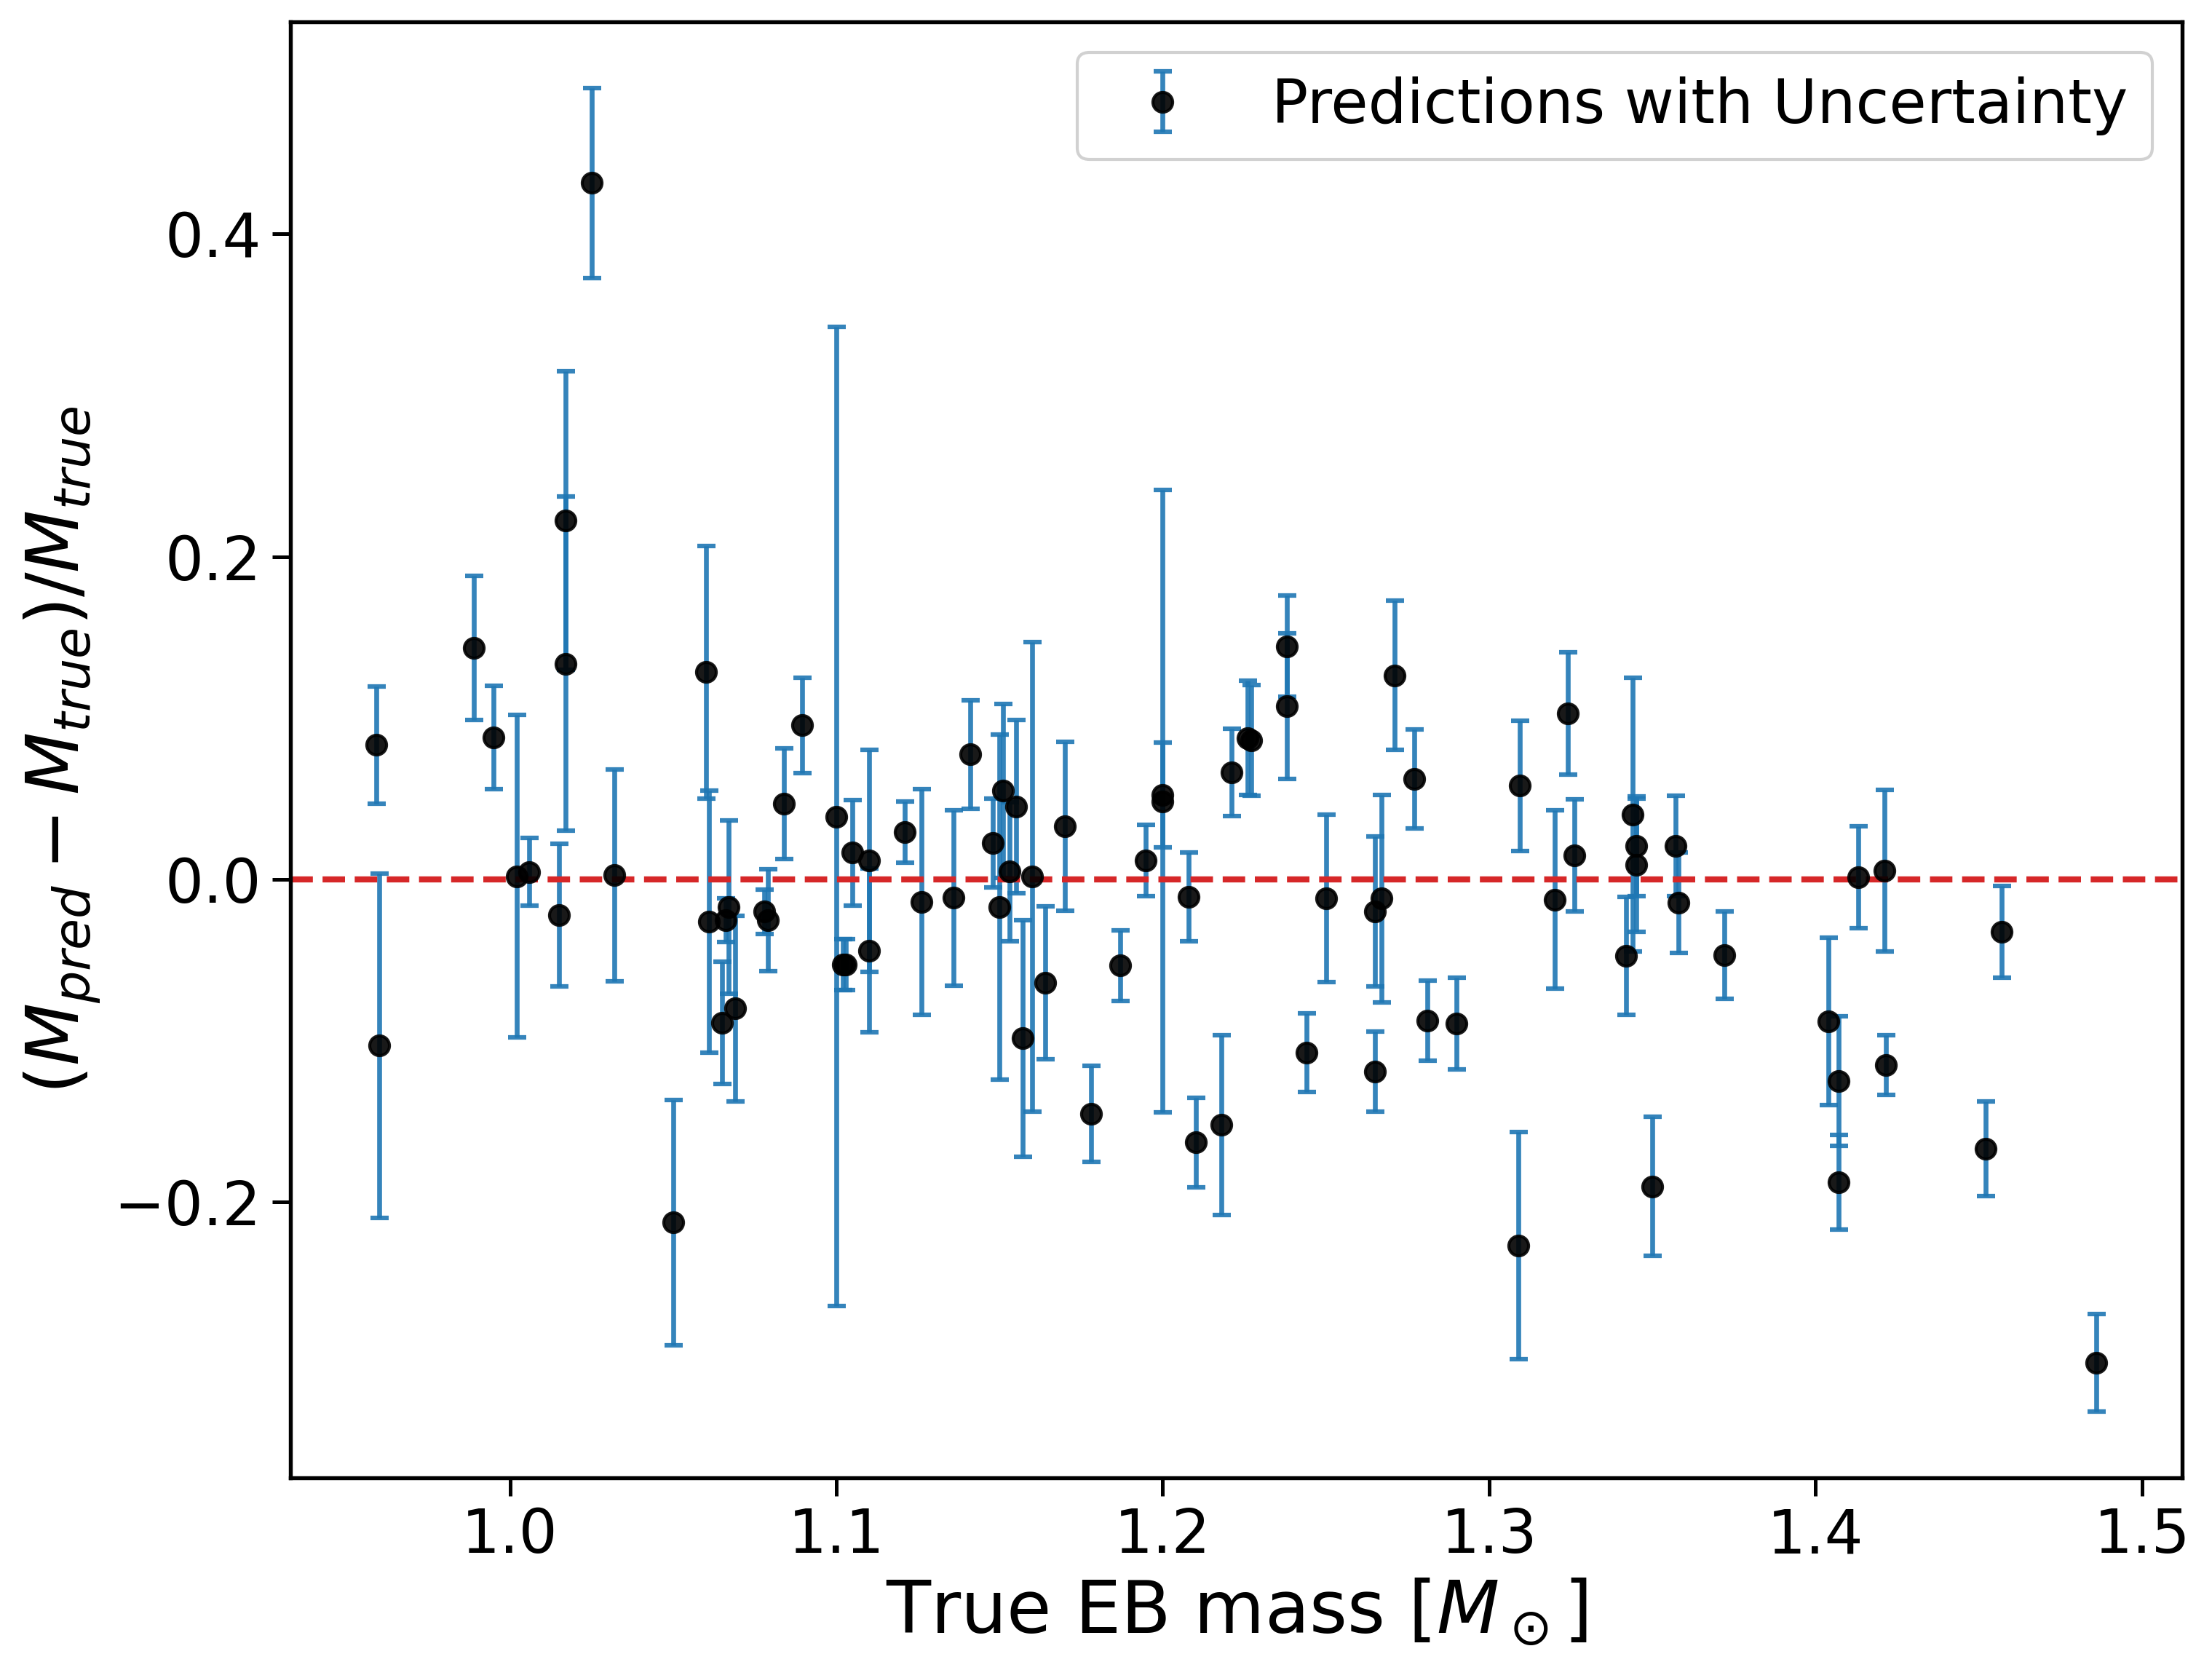
\includegraphics[width=\linewidth]{03_fractional_residual_vs_true_EB_mass.png}
    \caption{Fractional residuals.}
    \label{fig:dataset_D_mass_residuals}
\end{subfigure}
\hfill
\begin{subfigure}[t]{0.35\textwidth}
    \centering
    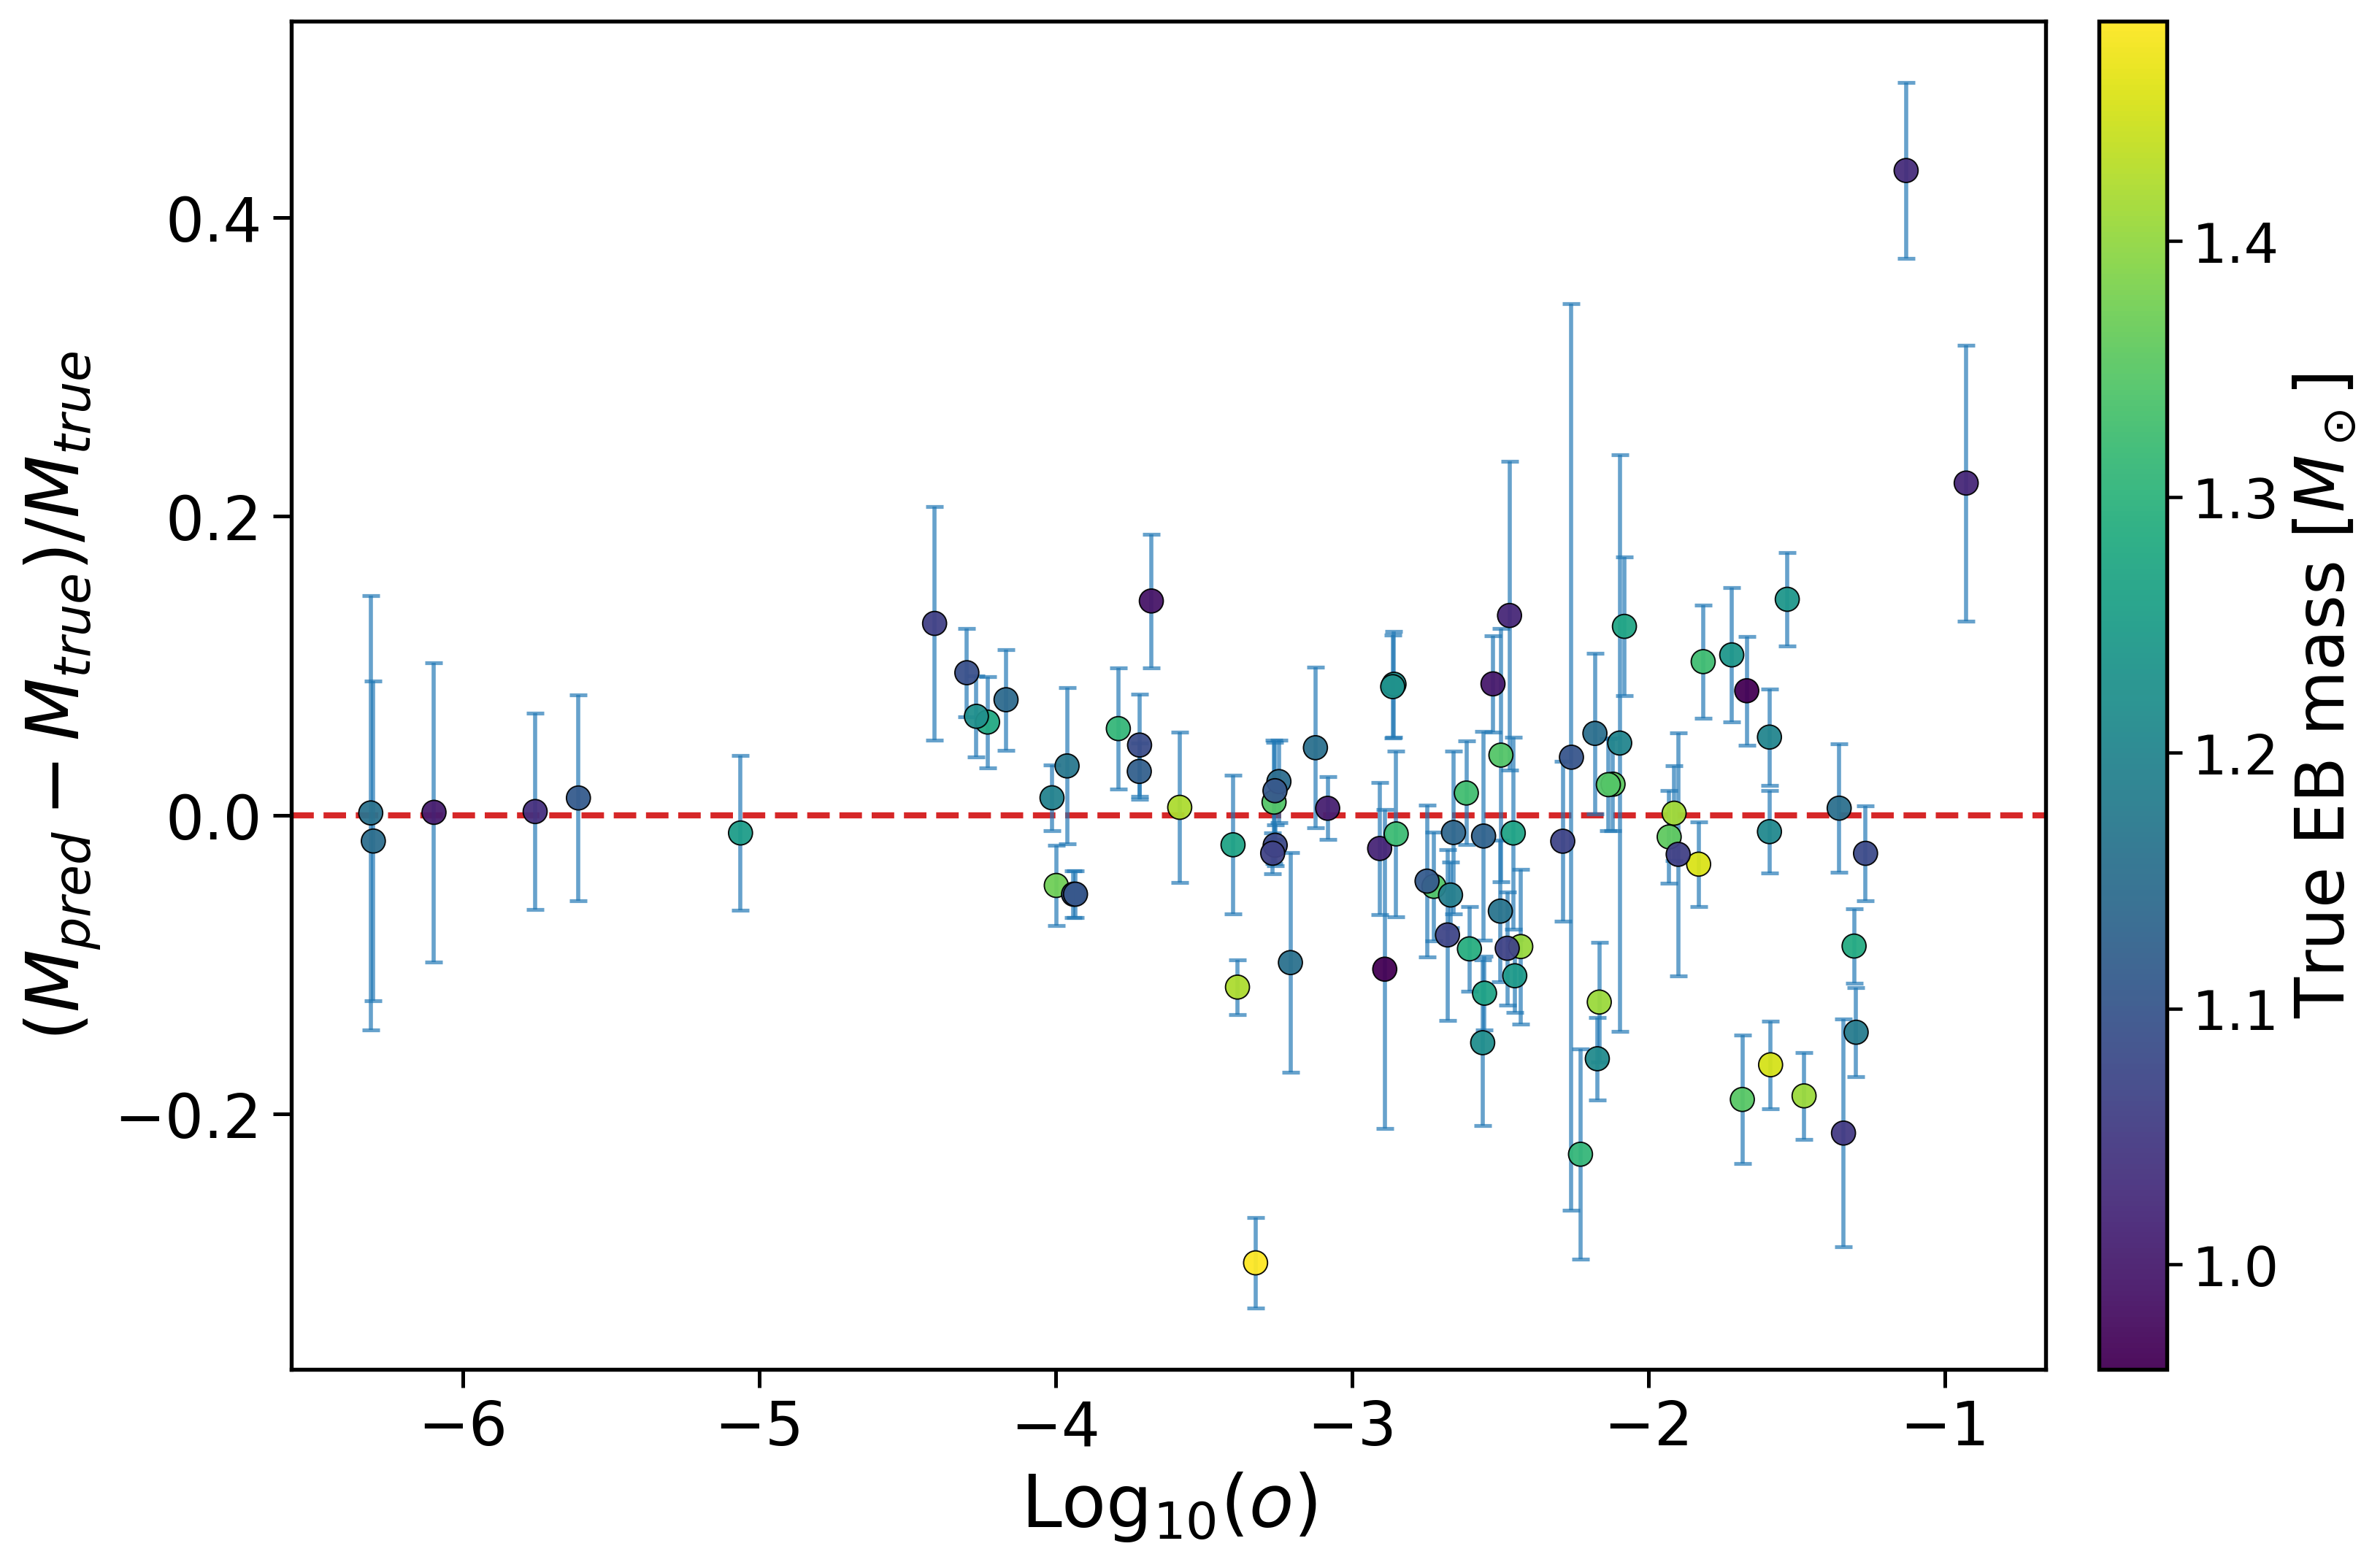
\includegraphics[width=\linewidth]{05_fractional_residual_vs_log10_oblateness_mass_colored.png}
    \caption{Fractional residuals, colour-coded by true mass.}
    \label{fig:dataset_D_o_residuals_mass_colored}
\end{subfigure}

\caption{Mass-prediction performance and mass dependence of the BHS residuals for the selected eclipsing-binary sample. The model uses $T_{\mathrm{eff}}$, $L$, $\log g$ and $[\mathrm{Fe}/\mathrm{H}]$ as input parameters. The left panel compares predicted and reference EB masses, the central panel shows the corresponding fractional residuals as a function of true mass, and the right panel shows the fractional residuals as a function of stellar oblateness $o$, colour-coded by true mass. Error bars show the propagated predictive uncertainty, and the dashed red line marks zero residual. The sample contains $n=85$ stars.}
\label{fig:dataset_D_mass}

\end{figure}

To test the dependence of the residuals on the different input parameters, a multivariable linear regression was performed on the eclipsing-binary residuals. Each feature, together with $o$ and $M$, was assigned a regression coefficient, $\beta$, quantifying its influence on the residual behaviour. Since the predictors were standardised, the coefficients can be directly compared.

The signed residuals are not significantly associated with oblateness, with $\beta_{\log o} = 0.002 \pm 0.005$, consistent with zero; $o$ does not introduce an overall positive or negative bias in the predictions. Instead, the signed residuals are mainly associated with the stellar parameters themselves. As already seen in Figure \ref{fig:dataset_D_mass}, mass affects the tendency towards overprediction or underprediction, with $\beta_M = -0.108 \pm 0.005$. Other relevant contributions are found for $T_{\mathrm{eff}}$, with $\beta_{T_{\mathrm{eff}}} = 0.077 \pm 0.007$, and for $[\mathrm{Fe}/\mathrm{H}]$, with $\beta_{[\mathrm{Fe}/\mathrm{H}]} = 0.048 \pm 0.002$.

The result changes when the absolute fractional residual is used as the response variable. In this case, $\log o$ is the only statistically significant predictor, with $\beta_{\log o} = 0.030 \pm 0.012$. Since the predictors are standardised, this means that a one-standard-deviation increase in $\log o$ is associated with an increase of about $3.0$ percentage points in $|\delta M|$. The remaining predictors are not significant in this regression.

The uncertainty calibration also suggests that eclipsing-binary stars are harder to predict than stars drawn from the training distribution, since an additional source of scatter appears when the asteroseismic-trained model is applied to eclipsing binaries. Only $30/85$ stars, or $35.3\%$, have their true mass within $1\sigma$ of the predictive interval.

\section{Conclusions} \label{sec:conclusions}

This work employed an uncertainty-aware stacking approach to obtain posterior predictive distributions for stellar masses using probabilistic machine-learning models. Three level-0 models, BART, HBNN and GP, were combined through Bayesian Hierarchical Stacking. The training set was constructed from high-quality reference catalogues based mainly on asteroseismology, detached eclipsing binaries and interferometry. The starting point was the 726 main-sequence-star catalogue of \citet{moya2018}, which was extended with recent literature sources published from 2018 onwards. After cleaning and cross-matching the samples, the final usable set consisted of 767 main-sequence stars, all of which had $M$, $T_{\mathrm{eff}}$, $L$, $[\mathrm{Fe}/\mathrm{H}]$ and $\rho$; 729 also had $\log g$, and 295 had $o$.

The first experiment tested the models on FGK-type stars, since this was the dominant stellar population in the final sample. Using a $20\%$ holdout set yielded mean absolute relative differences between predicted and reference masses which were all close to $5\%$, with the level-1 BHS model giving the best overall performance. HBNN and BART showed a systematic tendency to pull predictions towards approximately $1.25\,M_\odot$, where the training set is most densely populated. In contrast, GP showed no clear mass-dependent bias, although it produced a small number of outliers with unphysically large predictive uncertainties. The stacking model benefited from the complementary behaviour of the level-0 predictors and achieved an MRD of $0.20\%$, indicating negligible global bias.

The second experiment focused on a feature set with reduced model dependence, using $T_{\mathrm{eff}}$, $L$ and $[\mathrm{Fe}/\mathrm{H}]$ to estimate stellar masses. The qualitative behaviour of the three level-0 models and the stacking model remained similar to that found in the previous experiment, although the predictive precision worsened by approximately two percentage points. The models also showed a small overpredicting tendency, with the BHS model giving an MRD of $-1.36\%$. The predictions were then compared with evolutionary-grid estimates based on PARSEC \citep{bressan2012} and with linear-relation masses presented by \citet{moya2018}. The three approaches gave broadly compatible, but not identical results. A natural continuation of this analysis would be to combine all three approaches within a single stacking framework, so that the final estimate can benefit from the strengths of each method.

The third experiment showed that models trained on approximately single-star data can be transferred to eclipsing-binary components, but not without limitations. The oblateness parameter $o$ was introduced to quantify the degree of interaction between the two components, and the models were trained only on the assembled asteroseismic sample. The differences between the predicted and reference masses for eclipsing-binary stars were then analysed as a function of $o$. For the selected sample of 85 eclipsing-binary stars, oblateness did not introduce a significant signed mass bias, with $\beta_{\log o} = 0.002 \pm 0.005$. However, it did increase the absolute residuals, with $\beta_{\log o} = 0.030 \pm 0.012$, indicating a loss of precision rather than a systematic loss of accuracy. A practical transition point was found around $o \sim 0.01$, above which the residual scatter becomes large enough for the predictions to be considered less reliable.

\subsection*{Conclusiones}
\medskip
{\itshape
\noindent Este trabajo tom\'o un enfoque de stacking con tratamiento expl\'icito de incertidumbres para obtener distribuciones predictivas posteriores de masas estelares mediante modelos probabil\'isticos de machine learning. Tres modelos de nivel 0, BART, HBNN y GP, fueron combinados mediante Bayesian Hierarchical Stacking. El dataset de entrenamiento se construy\'o a partir de cat\'alogos de referencia de alta calidad, basados principalmente en astrosismolog\'ia, binarias eclipsantes e interferometr\'ia. El punto de partida fue el cat\'alogo de 726 estrellas de la secuencia principal recopilado por \citet{moya2018}, que se ampli\'o con fuentes bibliogr\'aficas recientes publicadas a partir de 2018. Tras la limpieza y el cruce de las muestras, el conjunto final utilizable qued\'o formado por 767 estrellas de la secuencia principal, todas ellas con $M$, $T_{\mathrm{eff}}$, $L$, $[\mathrm{Fe}/\mathrm{H}]$ y $\rho$; 729 tambi\'en ten\'ian $\log g$, y 295 ten\'ian $o$.

El primer experimento evalu\'o los modelos en estrellas de tipo FGK, dado que esta era la poblaci\'on estelar dominante en la muestra final. Utilizando un conjunto de prueba reservado del $20\%$, las diferencias relativas absolutas medias entre las masas predichas y las masas de referencia fueron todas pr\'oximas al $5\%$, con el modelo de stacking proporcionando el mejor rendimiento global. HBNN y BART mostraron una tendencia sistem\'atica a desplazar las predicciones hacia aproximadamente $1.25\,M_\odot$, donde el conjunto de entrenamiento se muestra m\'as densamente poblado. En cambio, GP no mostr\'o un sesgo claro dependiente de la masa, aunque produjo un reducido n\'umero de predicciones con incertidumbres f\'isicamente inveros\'imiles. El modelo de stacking se benefici\'o del comportamiento complementario de los predictores de nivel 0 y alcanz\'o un MRD de $0.20\%$, lo que indica un sesgo global despreciable.

El segundo experimento se centr\'o en un conjunto de variables de entrada con menor dependencia de modelos, utilizando $T_{\mathrm{eff}}$, $L$ y $[\mathrm{Fe}/\mathrm{H}]$. El comportamiento cualitativo de los tres modelos de nivel 0 y del modelo BHS se mantuvo similar al encontrado en el experimento anterior, aunque la precisi\'on predictiva empeor\'o en aproximadamente dos puntos porcentuales. Los modelos tambi\'en mostraron una leve tendencia a la sobrepredicci\'on, con el modelo BHS dando un MRD de $-1.36\%$. Las predicciones se compararon posteriormente con estimaciones basadas en modelos estelares de PARSEC \citep{bressan2012} y con predicciones mediante las relaciones lineales presentadas por \citet{moya2018}. Los tres enfoques dieron resultados compatibles, aunque no id\'enticos. La continuaci\'on natural de este an\'alisis ser\'ia combinar los tres enfoques dentro de un \'unico marco de stacking, de modo que la estimaci\'on final pueda beneficiarse de las fortalezas de cada m\'etodo.

El tercer experimento mostr\'o que los modelos entrenados con datos de estrellas individuales pueden transferirse a componentes de binarias eclipsantes, aunque no sin limitaciones. El par\'ametro de oblaticidad $o$ se introdujo para cuantificar el grado de interacci\'on entre las dos componentes, y los modelos se entrenaron \'unicamente con la muestra astrosismol\'ogica recopilada. Las diferencias entre las predicciones de masas y los valores de referencia para las estrellas binarias eclipsantes se analizaron entonces como funci\'on de $o$. Para la muestra seleccionada, 85 estrellas binarias eclipsantes, la oblaticidad no introdujo un sesgo signado de masa significativo, con $\beta_{\log o} = 0.002 \pm 0.005$. Sin embargo, s\'i aument\'o los residuos absolutos, con $\beta_{\log o} = 0.030 \pm 0.012$, lo que indica una p\'erdida de precisi\'on m\'as que una p\'erdida sistem\'atica de exactitud. Se encontr\'o un punto de transici\'on pr\'actico alrededor de $o \sim 0.01$, por encima del cual la dispersi\'on de los residuos se vuelve suficientemente grande como para considerar las predicciones menos fiables.
}


\bibliographystyle{aasjournal}
\bibliography{references}

\end{document}
\endinput}
\fi
\BayeStarMLMaybeInputMain

\documentclass[paper=a4, fontsize=12pt]{scrartcl}

\usepackage[british]{babel}
\usepackage[utf8]{inputenc}
\usepackage[T1]{fontenc}

% Mathematics
\usepackage{amsmath, amsfonts, amssymb, amsthm}
\usepackage{accents}
\usepackage{cancel}

% Units
\usepackage{siunitx}

% Figures and tables
\usepackage{graphicx}
\usepackage{epstopdf}
\usepackage{float}
\usepackage[labelfont=bf]{caption}
\usepackage{subcaption}
\captionsetup[table]{labelsep=period,singlelinecheck=false}

% Layout and formatting
\usepackage[a4paper,margin=22mm]{geometry}
\usepackage{sectsty}
\allsectionsfont{\normalfont\scshape\bfseries}
\sectionfont{\normalfont\Large\scshape\bfseries}
\setlength\parindent{15pt}

\usepackage{fancyhdr}
\pagestyle{fancy}
\fancyhead{}
\fancyfoot[L]{}
\fancyfoot[C]{}
\fancyfoot[R]{\thepage}
\renewcommand{\headrulewidth}{0pt}
\renewcommand{\footrulewidth}{0pt}
\setlength{\headheight}{13.6pt}

\usepackage{setspace}
\setstretch{1.15}

\newcommand{\horrule}[1]{\rule{\linewidth}{#1}}

% Other packages
\usepackage{lipsum}
\usepackage{xcolor}
\usepackage{makeidx}
\usepackage{fancybox}
\usepackage{tikz}
\usepackage[most]{tcolorbox}
\usepackage{multicol}

% Background
\usepackage[pages=some]{background}
\backgroundsetup{
 scale=1,
 color=black,
 opacity=1,
 angle=0,
 contents={
 
\includegraphics[height=\paperheight]{Figuras/Fondo.pdf}
 }
}
\usepackage{wallpaper}

% Bibliography
\usepackage[round,authoryear]{natbib}
\setlength{\bibsep}{0pt plus 0.2ex}
\providecommand{\bibfont}{}
\renewcommand{\bibfont}{\normalfont\normalsize\setstretch{1.0}}

% Hyperref should be near the end
\usepackage[hidelinks=true, hyperfootnotes=false]{hyperref}



\begin{document}
% !TeX root = ./main.tex

\begin{titlepage}
   \thispagestyle{empty}
   \noindent\raisebox{0pt}[0pt][0pt]{%
      
\includegraphics[width=10.5cm]{portada-TFG-LaTeX/marca-Facultat-Fisica-UV-1-linia.pdf}%
   }\par
   \vspace{8.5cm}
   {\centering
      {\bfseries\LARGE Treball de Fi de Grau en F\'isica}\par
      \rule{\textwidth}{1.5pt}\par
      \vspace{4.5cm}
      {\bfseries\LARGE Training of Machine Learning Models for Stellar Characterization}\par
   }
   \vfill
   {\raggedleft
      June 2026\par
      \vspace{\baselineskip}
      Alumne/a: Nicol\'as Georgak\'opulos Franch\par
      \vspace{\baselineskip}
      Tutor/a: Andr\'es Moya Bed\'on\par
   }
\end{titlepage}

\iffalse
Original cover kept for reference.

\begin{titlepage}
% Fondo Portada
   \AddToShipoutPicture*{\put(0,0){
\includegraphics[scale=1]{Figuras/Fondo.pdf}}}
	\noindent
	\vspace{1mm}
 %%
 \centering
 {
\includegraphics[width=0.28\textwidth]{Figuras/uv.png}\par}
 \vspace{0.5cm}
 {\bfseries\LARGE Universitat de València \par}
 %\vspace{0.5cm}
 {\scshape\Large Physics BSc \par}
 \vspace{1.5cm}
 {\scshape\Huge Trabajo de Fin de Grado: \par}
 \vspace{0.5cm}
 {\scshape\Huge \textbf{TRAINING OF MACHINE LEARNING/ARTIFICIAL INTELLIGENCE MODELS FOR STELLAR CHARACTERIZATION} \par}
 \vspace{3cm} \vfill
 {\Large Tutor: \textit{Andrés Moya Bedón} \\ \hspace{3cm}\textit{} \par}
 \vfill
 {\Large \textbf{Nicolás Georgakópulos} \par}
 \end{titlepage}
\fi

\newpage

\begingroup
\setlength{\parindent}{0pt}
\noindent\resizebox{0.48\textwidth}{!}{%
\begin{minipage}[t]{0.785\textwidth}
    \setstretch{0.95}
    \begin{center}
        \bfseries Abstract
    \end{center}
    Reliable stellar masses are required for stellar astrophysics and for the interpretation of exoplanet observations, but direct and homogeneous mass determinations are available only for limited samples. This work presents an uncertainty-aware machine-learning study of main-sequence stellar mass prediction based on a high-quality sample of 767 stars assembled mainly from eclipsing binaries, asteroseismic stars and interferometric benchmark stars. Bayesian Additive Regression Trees, a two-process heteroscedastic sparse Gaussian Process and a Hierarchical Bayesian Neural Network are trained as level-0 predictors, whose posterior predictive distributions are combined through Bayesian Hierarchical Stacking.

    \par\smallskip
    For FGK-type stars, using $T_{\mathrm{eff}}$, $\rho$ and $[\mathrm{Fe}/\mathrm{H}]$ as input features, the stacking model reaches a mean absolute difference below $5\%$ on a holdout test set, while showing no clear mass-dependent bias. The same framework is then applied to eclipsing-binary components using $T_{\mathrm{eff}}$, $L$, $\log g$ and $[\mathrm{Fe}/\mathrm{H}]$, in order to test whether tidal distortion affects mass predictions transferred from a purely asteroseismic training sample. For the selected sample of 85 binaries, oblateness does not produce a significant signed bias, but it is associated with an increase in the absolute mass residuals, indicating a loss of precision rather than a systematic loss of accuracy. Finally, an experiment motivated by the ESA ARIEL mission uses $T_{\mathrm{eff}}$, $[\mathrm{Fe}/\mathrm{H}]$ and $L$, excluding $\log g$ to reduce direct dependence on stellar evolutionary models, and yields mean absolute differences below $7\%$. The comparison with stellar-grid and linear-relation masses shows that the methods give broadly consistent but not identical results, supporting the use of probabilistic stacking as a data-driven tool for stellar-mass estimation with reduced model dependence and explicit uncertainty propagation.
\end{minipage}}\hfill
\resizebox{0.48\textwidth}{!}{%
\begin{minipage}[t]{0.785\textwidth}
    \setstretch{0.95}
    \itshape
    \begin{center}
        Resumen
    \end{center}
    La obtenci\'on fiable de masas estelares es necesaria para la astrof\'isica estelar y para la interpretaci\'on de observaciones de exoplanetas, pero su determinaci\'on directa y homog\'enea s\'olo es posible mediante muestras limitadas. Este trabajo presenta un estudio mediante machine learning con tratamiento expl\'icito de incertidumbres para la predicci\'on de masas de estrellas de la secuencia principal, basado en una muestra de alta calidad de 767 estrellas, construida principalmente a partir de binarias eclipsantes, m\'etodos astros\'ismicos y estrellas de referencia interferom\'etricas. Bayesian Additive Regression Trees, una Red Neuronal Bayesiana Jer\'arquica y un Gaussian Process disperso heteroced\'astico de dos procesos se entrenan como predictores de nivel 0, cuyas distribuciones predictivas posteriores se combinan mediante Bayesian Hierarchical Stacking.

    \par\smallskip
    Para estrellas de tipo FGK, usando $T_{\mathrm{eff}}$, $\rho$ y $[\mathrm{Fe}/\mathrm{H}]$ como variables de entrada, el modelo de stacking alcanza una diferencia media absoluta inferior al $5\%$ en un conjunto de prueba reservado a partir del dataset original, sin mostrar un sesgo signado claro dependiente de la masa. El mismo marco se aplica despu\'es a componentes de binarias eclipsantes usando $T_{\mathrm{eff}}$, $[\mathrm{Fe}/\mathrm{H}]$, $L$ y $\log g$, con el objetivo de comprobar si la distorsi\'on por mareas afecta a las predicciones de masa transferidas desde una muestra de entrenamiento puramente astros\'ismica. Para la muestra seleccionada de 85 binarias, la oblaticidad no produce un sesgo signado significativo, pero s\'i est\'a asociada con un aumento de los residuos absolutos de masa, lo que indica una p\'erdida de precisi\'on m\'as que una p\'erdida sistem\'atica de exactitud. Finalmente, un experimento motivado por la misi\'on ARIEL de la ESA usa $T_{\mathrm{eff}}$, $[\mathrm{Fe}/\mathrm{H}]$ y $L$, excluyendo $\log g$ para reducir la dependencia directa de modelos de evoluci\'on estelar, y obtiene diferencias medias absolutas inferiores al $7\%$. La comparaci\'on con masas obtenidas mediante modelos de evoluci\'on estelar y relaciones lineales muestra que los m\'etodos proporcionan resultados ampliamente consistentes, aunque no id\'enticos, apoyando el uso del stacking probabil\'istico como herramienta basada en datos para la estimaci\'on de masas estelares con menor dependencia de modelos y propagaci\'on expl\'icita de incertidumbres.
\end{minipage}}
\par\vspace{0.05cm}
{\setstretch{0.7}\tableofcontents}
\endgroup
\newpage


\section{Introduction} \label{sec:introduction}

Machine-learning methods have become increasingly important in stellar astrophysics, particularly for stellar characterization \citep{moya2022}. Quantities such as stellar mass, radius, effective temperature, luminosity, surface gravity and metallicity determine the physical state and evolutionary stage of a star, and they also affect the interpretation of any planetary system orbiting it. Reliable stellar parameters are therefore required. However, the direct determination of these quantities is not always possible \citep{Serenelli2021}. Different observational methods constrain different stellar parameters with different levels of model dependence, and no single method provides complete coverage across all stellar types.

For stars lacking direct mass measurements, empirical relations and numerical regression methods provide a way to infer masses from other observable stellar parameters. With the development of artificial intelligence and machine learning, more flexible methods can now be used to model these relations \citep{moya2022}. Their usefulness depends not only on predictive accuracy, but also on their ability to represent uncertainty and on the quality of the data from which they learn.

This work adopts a Bayesian approach to machine-learning stellar-mass prediction. Input quantities with reported uncertainties are treated as probability distributions, allowing the models to propagate observational uncertainties into their posterior predictions. This is especially relevant when the models are applied to regions of parameter space that are sparsely represented in the training data. The models used in this work, described in Section \ref{sec:models}, are combined through Bayesian Hierarchical Stacking. This stacking approach assigns feature-dependent weights to the different predictors, allowing the final model to favour each method in the regions where it performs most reliably \citep{yao2022hierarchicalstacking}.

The resulting predictions depend strongly on the quality of the training data: precision, completeness and physical reliability of the stellar features used \citep{Serenelli2021}. For this reason, the training sample is built from reference methods that provide the most reliable available stellar parameters, mainly detached eclipsing binaries, asteroseismology and interferometry, as described in Section \ref{methods}. The literature sources used to build the final catalogue are carefully selected and processed in Section \ref{sec:data}.

The models are applied in three studies, presented in Section \ref{sec:results}. The first application provides a baseline assessment of the predictive accuracy and bias of each method, as well as of the improvement obtained through Bayesian Hierarchical Stacking. In addition, the limited coverage of low-mass M stars is approached indirectly through FGK-type stars in eclipsing-binary systems, since the latter are the most common type of stars in the training database. Following \citet{maxted2023benchmark}, accurate characterization of the FGK-type primary can help constrain the properties of the lower-mass companion. 

The second application is motivated by ESA's ARIEL space mission, for which accurate stellar characterization is required to interpret atmospheric observations of the exoplanets orbiting the studied stars. In this case, the mass estimates should be as independent as possible from stellar evolutionary models. The feature $\log g$ is therefore excluded because it may introduce a stronger dependence on stellar-evolution models \citep{tsantaki2018,Serenelli2021}. The resulting predictions are also compared with masses obtained from stellar evolutionary grids and with masses derived from linear relations in \citet{moya2018}.

Finally, this work examines whether eclipsing-binary components can be treated as approximately individual stars, for the purposes of mass prediction. To test this, asteroseismic stars are taken as a reference sample of approximately isolated stellar evolution. The models are trained only on asteroseismic stars, and then applied to eclipsing-binary components. The differences between the predicted and reference masses are analysed as a function of the oblateness parameter, used here as an indicator of binary interaction. This makes it possible to assess whether mass relations calibrated on individual stars remain valid for eclipsing-binary components, or whether increasing tidal distortion produces a measurable degradation in the predictions.

MIGHT DELETE THIS PARAGRPAH
Overall, this thesis combines catalogue construction, Bayesian machine learning and astrophysical validation tests in order to assess how reliably stellar masses can be inferred from observable stellar parameters. The emphasis is placed not only on predictive performance, but also on uncertainty calibration and model dependence.


\section{Machine Learning Models} \label{sec:models}



\subsection{Bayesian Framework for the Models} \label{sec:bayesian-inference}
%could the cafeteria reference be used gere?
Bayesian statistics treats unknown model quantities as uncertain variables. The information available before analysing the data is encoded in a prior distribution; after conditioning on the observations, this information is updated into a posterior distribution. In compact form, Bayes' theorem states that $p(\theta \mid \mathcal{D}) = p(\mathcal{D} \mid \theta)p(\theta)/p(\mathcal{D})$, where $\theta$ represents model parameters, $\mathcal{D}$ the data and $p(\mathcal{D})$ the evidence, which normalizes the posterior distribution. This is useful in scientific modelling because it makes assumptions explicit and allows uncertainty to be carried through the full inference process \citep{mcelreath2020rethinking}.

This framework is especially relevant for stellar characterization. The training data contain observational errors, correlations between stellar parameters and regions of sparse feature coverage in parameter space. In this context, the input stellar quantities used by the models are referred to as features. A Bayesian treatment is therefore not chosen only to obtain point predictions, but to quantify how reliable those predictions are. The models discussed in the following subsections use priors to regularize flexible functions and posterior inference to propagate both data uncertainty and model uncertainty into the final estimates \citep{chipman2010bart,rasmussen2006gpml,jospin2022bnn}.

For the models used here, the posterior distribution is usually too complex to evaluate analytically. Markov Chain Monte Carlo (MCMC) methods address this by constructing a sequence of dependent samples whose long-run distribution approximates the target posterior. A proposed move is accepted or rejected according to how compatible it is with the posterior, so the chain spends more time in high-probability regions without requiring an exhaustive search of the full parameter space \citep{hastings1970,bardenet2017mcmc}. However, because consecutive samples are correlated, practical MCMC requires convergence checks, an initial warm-up or burn-in period, and attention to the effective number of independent samples. Although computationally expensive, this sampling approach is well suited to the Bayesian models in this work because it provides a principled way to explore parameter uncertainty rather than collapsing the model to a single point estimation without error.

Rather than selecting a single best model, this work combines the predictions of independent level-0 models through Bayesian Hierarchical Stacking (BHS), as sketched in Figure \ref{fig:bhsarch}. In the following sections, a Bayesian Additive Regression Trees, a Gaussian Process and a
hierarchical Bayesian neural network model are described. The predictions yielded by these models can be passed to this first-level model, which assigns feature-dependent weights to each one, in order to optimize predictive performance.

\begin{figure}[H]
    \centering
    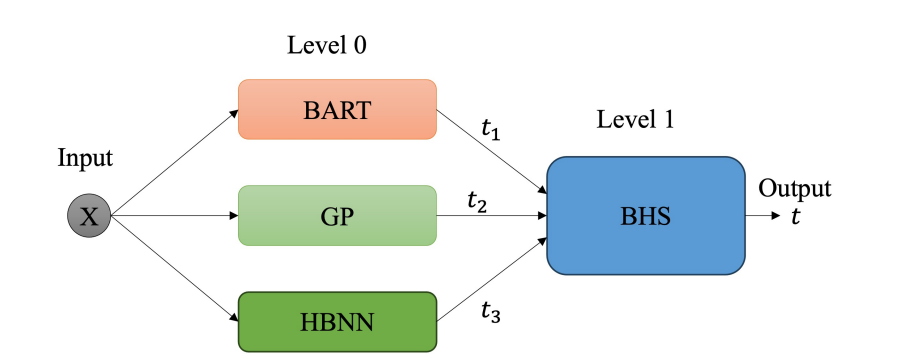
\includegraphics[width=0.65\linewidth]{stacking_arquitecture.png}
    \caption{Schematic architecture of the Bayesian Hierarchical Stacking model. The predictions from BART, GP and HBNN are combined through a first-level model that learns their relative weights.}
    \label{fig:bhsarch}
\end{figure}

\iffalse
ADD SOME BRIEF INTRO ABOUT BAYESIAN INFERENCE and statistics, PRIORS AND POSTERIORS, AND THE MODELS TO BE USED, WITHOUT NAMiNG THEM. NOT MORE Than ONE OR TWO PARAGRAPHS
Valuable source for this and other sections: Statistical Rethinking by Richard McElreath https://oceanrep.geomar.de/id/eprint/55819/1/Statistical%20Rethinking%202nd%20Edition.pdf. 
cafe example in page 413 is great to understand how a prior is learned from the data itself


W. K. Hastings, “Monte Carlo sampling methods usingMarkov chains and their applications,” Biometrika, vol. 57, no. 1, pp. 97–109, 04 1970 https://www2.stat.duke.edu/~scs/Courses/Stat376/Papers/Basic/Hastings1970.pdf


The objective of Markov Chain Monte Carlo (MCMC) methods is to construct a sequence of random samples (a Markov chain) where each state $S_i$ probabilistically depends exclusively on the preceding state $S_{i-1}$. Rather than executing a computationally intractable random grid search across all independent Gaussian distributions, the algorithm initiates at a random coordinate and proposes a sequential step (there's yt videos about this). If the proposed step moves toward a region of higher probability density within the posterior distribution, it is accepted. If it moves toward a less probable region, it is typically rejected, and the chain records the current position again. This mechanism allows the algorithm to efficiently map complex distributions with far fewer iterations than brute-force random sampling.

This sequential dependency introduces inherent drawbacks. Because $S_i$ is physically tethered to $S_{i-1}$, successive samples are highly autocorrelated and do not represent strictly independent draws from the posterior. To mitigate this, algorithms require an initial ``burn-in'' period (a large set of early iterations that are permanently discarded to allow the chain to reach the stationary distribution). Following burn-in, the chain must be thinned, storing only a subsampled fraction of the sequence (typically retaining only every $N$-th iteration) to approximate independent sampling. Despite these computational expenses, MCMC remains the optimal framework for sampling exact posterior distributions in highly parameterized deep learning models (R. Bardenet, A. Doucet, and C. Holmes, ``On Markov Chain Monte Carlo methods for tall data,'' J. Mach. Learn. Res., vol. 18, no. 1, pp. 1515–1557, Jan. 2017).

By tracking multiple independent Markov chains simultaneously, the algorithm thoroughly maps the hyperparameter space. This process inherently captures the learned covariance between variables, enforcing physical and mathematical limits on the parameter combinations that the respective probabilistic models evaluate.

\fi

\subsection{Bayesian Additive Regression Trees (BART)}
Among the three level-0 models used in this work, the practical deployment of the BART framework is mathematically and computationally the most straightforward, since its architecture requires relatively few tuning choices \citep{hill2020}. To understand the ensemble, the mechanics of a single regression tree must be defined. A tree recursively partitions the dataset by evaluating binary thresholds across input variables (e.g. $T_{\mathrm{eff}} < 5000\,\mathrm{K}$). At each step, the algorithm selects the threshold that maximizes the homogeneity of the target variable in the resulting subsets. When predicting for a new observation, the input traverses this learned path of decisions until it reaches a terminal node, or ``leaf''. The target variable prediction associated with that leaf is simply the mean value of the training points that occupy that specific terminal node.

% Explanation of "At each step, the algorithm selects the threshold that maximizes the homogeneity of the target variable in the resulting subsets.": Assume a parent node contains five stars with known masses: $[1.0, 1.1, 1.2, 5.0, 5.2]$.The algorithm tests possible splitting thresholds on an input variable (e.g., Effective Temperature).Split Option A: Creates Subset 1 $[1.0, 5.0]$ and Subset 2 $[1.1, 1.2, 5.2]$. Both subsets contain extreme high and low values. Internal variance is high. Homogeneity is low. The algorithm rejects this threshold.Split Option B: Creates Subset 1 $[1.0, 1.1, 1.2]$ and Subset 2 $[5.0, 5.2]$. The values inside Subset 1 are nearly identical to each other. The values inside Subset 2 are nearly identical to each other. Internal variance is minimized. Homogeneity is maximized. The algorithm selects this threshold.

The Bayesian Additive Regression Trees framework, introduced by \citet{chipman2010bart}, employs a sum-of-trees architecture to approximate complex non-linear functions. A Random Forest constructs an ensemble of deep, independent regression trees. By training each one of such trees on a random sample of the dataset and averaging the predictions of all of them, it produces a final output which reduces variance. BART follows this dataset subsampling logic, but the final predictions are not the average of the independent models, but the cumulative sum of the terminal node values across all interdependent trees in the ensemble. Therefore, in Random Forests every tree is a strong learner which produces an absolute value prediction for the target; while in BART the trees are weak learners, which just produce a part of the answer \citep{chipman2010bart}.

% Explanation of last part: in RF, you have 3 trees that give 1.9, 2.0 and 2.1. in BART, they giuve 1.5, 0.2 and 0.3.

This weak learner approach is mathematically guaranteed by regularisation priors, which constrain the size and structural influence of each tree. These mathematical penalties prevent any single tree component from dominating the overall model, thereby preserving the functional and computational advantages of the additive representation. Left unconstrained, the algorithm naturally drives individual trees to grow massive in pursuit of tighter data fits \citep{chipman2010bart}. The priors counteract this by forcing each tree to function as a weak learner, modelling only a restricted subset of the underlying function. This way, each tree provides only a small part of the predictor space, not a prediction itself.

Since each individual tree recursively partitions the predictor space utilising binary decision rules, the overall capacity and complexity of the model depends on the total number of trees. Predictive performance generally improves as this quantity increases, eventually reaching an asymptote.

Model optimisation follows the Bayesian backfitting MCMC scheme introduced in Section \ref{sec:bayesian-inference}. During each sweep, the algorithm updates one tree conditional on the partial residual left by the rest of the ensemble, proposing local changes such as growing, pruning or modifying a split. Repeating this process samples plausible tree structures and terminal-node values rather than selecting a fixed ensemble \citep{chipman2010bart}.

Crucially for stellar characterization, where uncertainty of the input features is a dominant factor, the framework used in this work accommodates an errors-in-variables approach. Inputs are not treated as static, exact measurements; rather, they are modeled as latent variables characterised by a Gaussian distribution whose variance is fixed by the observational uncertainties. This allows the model to account for the diverse uncertainties present across the entire star catalogue.



\subsection{Two-process Heteroscedastic Sparse Gaussian Process (GP)}
In classical parametric modelling, the functional form of the predictor is fixed in advance and inference is performed over its parameters. A Gaussian Process (GP) takes a different approach: it defines a probability distribution over possible functions. Any finite set of function values is assumed to follow a joint Gaussian distribution, so the model is specified by a mean function and a covariance function, or kernel. In many applications, the covariance function carries most of the information, while the mean function can be set to zero. Therefore, the main modelling choices are the prior covariance structure and the observational noise model, rather than an explicit fixed equation for the underlying function \citep{mackay1998gp,rasmussen2006gpml}.



% First, understand a multivariate gaussian: many variables, each in a gaussian distribution. A multivariate gaussian lives in a vector space, since each individual point has many components: point x has (x1, x2,...), point y has (y1, y2,...) and the gaussians followed are the gaussian conformed by (x1, y1...) the gaussian formed by (x2, y2...) and so on. If we extend these multivariate gaussian from a finite vector space to a continuous function space, we have a Gaussian Process (GP), where the elements are the functions (one element might be f(x, y) = sin x + y, the other might be g(x, y) = 2x + 6y). And the gaussian distributions are followed by the functions evaluated at the same points (f(2, 5) and g(2, 5); f(1, 0) and g(1,0)...). 

% The result of a gaussian distribution of vectors is a vector: the components of this result vector follow a gaussian, so for each iteration different numbers will be obtained, but overall they form a gaussian. The result of a gaussian distribution of functions is a function, where each point of the variable space follows a gaussian. But again, the result of an iteration is just a function with a fixed number for every coordinate in space. But these fixed numbers come from a gaussian dsitribution.


Training a GP therefore amounts to selecting a kernel and inferring its constraints, usually referred to as hyperparameters. The amplitude of the kernel controls the overall scale of the functions, and its length-scale controls how rapidly function values can change along the input axes. In this work, the kernel is chosen to favour smooth functions: nearby points in the input space are strongly correlated, while the correlation decreases as their separation increases. Large length-scales are thus dominant, since they produce slowly varying functions \citep{rasmussen2006gpml}.

% (additional info at the end of the text, to help you explain it better in the presentation)

% FINAL VERSION: MIGHT ERASE LAST SENTENCE OF THIS PARAGRAPH
To prevent the model from choosing unphysical hyperparameter values, priors are placed on the kernel length-scales and amplitudes. The version used in this work is the Automatic Relevance Determination (ARD) kernel, where each input dimension has its own length-scale, rather than sharing a single one. Dimensions with little predictive information can therefore be assigned very large length-scales, making them contribute less to the covariance structure \citep{rasmussen2006gpml}. The priors regularise this process by keeping the length-scales compatible with the spacing and span of the training data, while weakly informative amplitude priors avoid variances that collapse to zero or diverge.

The standard GP formulation usually assumes homoscedastic observational noise, meaning a single constant noise variance across the dataset. Stellar catalogues, however, contain measurements with uncertainties that vary between stars and between parameters. To account for this, the model used in this work follows a two-process heteroscedastic construction: one GP, $f(\boldsymbol{x})$, represents the latent predictive mean as a function of the stellar parameters, while a second GP, $g(\boldsymbol{\epsilon})$, models the logarithm of the noise variance from the reported measurement errors. This allows the predictive uncertainty to vary across the input space instead of being forced into a single global noise level \citep{le2005heteroscedasticgp}.

This flexibility comes with a computational cost. Because the kernel compares each data point with every other one, standard GP inference constructs an $N \times N$ covariance matrix; its diagonal terms describe each point's variance, while the off-diagonal terms encode similarity between different observations \citep{rasmussen2006gpml}. GP inference scales as $\mathcal{O}(N^3)$ because it requires operations on the full covariance matrix. To make inference feasible, both processes $f(\boldsymbol{x})$ and $g(\boldsymbol{\epsilon})$ are represented through a sparse approximation with $M$ inducing points, which act as representatives of the entire training set. Predictive covariances are therefore computed through the inducing set rather than directly through all pairwise relations between the $N$ observations, reducing the computational complexity to approximately $\mathcal{O}(NM^2)$ \citep{quinonero2005sparsegp}. Even so, Gaussian Processes can remain computationally demanding for large datasets.

The model is treated in a fully Bayesian way. As described in Section \ref{sec:bayesian-inference}, MCMC sampling explores plausible kernel hyperparameters, inducing variables and noise structures rather than fixing them at a single point with no uncertainty. Predictions are then averaged over these samples, propagating measurement and model uncertainty into the reported intervals.


% Additional info on the kernel function. First, picture the weight space. You have a set of data x, that we can fit to a linear regression model. But if we first apply a fixed function to these data, we can do the regression in the results (weight) space. We execute standard, computationally cheap linear matrix algebra in the 3D feature space, but the result projects back into the 1D input space as a non-linear parabola. Weight space allows linear algorithms to model non-linear geometries. We can extend the definition to function space: specifying a weight space and performing linear regression with a distribution of weights is mathematically identical to directly evaluating a kernel function between two points (evaluating the function itself, not fixed in this case).

% Additional way of understanding the length scale $\ell$: how far does one need to move (along a particular axis) in the input space for the function values to become uncorrelated.



\subsection{Hierarchical Bayesian Neural Network (HBNN)}
% "Traditional NN," "classical NN," and "point-estimate NN" all refer to the exact same thing: a standard neural network that uses fixed numbers for its weights, rather than probability distributions. ANN is just the broad category

% A bayesian neural network (BNN) is a stochastic artificial neural network (ANN) trained using Bayesian inference. So  just training an ANN with some probability distribution.


% other source: UNUSED: Weight Uncertainty in Neural Networks" by Blundell et al. (2015), USED a lot: Jospin et al. (2022) "Hands-on Bayesian Neural Networks - A Tutorial for Deep Learning Users"

% Good way of initially understanding neural newtorks:

% At its core, a neural network is an intricate sequence of mathematical operations. Data flows through hidden layers where every "neuron" calculates a sum by multiplying incoming data by adjustable **weights** and adding a baseline **bias**. To ensure the network can understand complex, real-world patterns rather than just plotting flat lines, this sum is passed through an activation function like **ReLU** (bc the other things are just linear). ReLU acts as a simple non-linear threshold (typically passing positive numbers through directly while turning any negative numbers into zero) which fundamentally allows the network to bend and shape its mathematical understanding of the data.

% The "learning" aspect is simply the automated, ongoing tuning of these equations to emulate reality. When a network first makes a prediction, its random weights produce an incorrect answer. By comparing its mathematical output to the true, real-world answer, the system calculates the exact error and uses a process called **backpropagation** to work backward through the layers, systematically tweaking every single weight and bias. After thousands or millions of these microscopic adjustments, the network's internal math becomes perfectly balanced to reliably transform new inputs into highly accurate predictions.

At its core, an artificial neural network is a sequence of mathematical operations arranged in layers. Neural networks are used to approximate non-linear relations by applying successive linear transformations and non-linear activation functions to the input data. In a standard network, the weights and biases in each layer are fitted as fixed point estimates. This can provide accurate predictions, but it does not naturally represent uncertainty in the model parameters and may produce overconfident results outside the region well covered by the training data \citep{jospin2022bnn}. 

Bayesian Neural Networks (BNNs) address this limitation by assigning probability distributions to the weights and biases instead of single values. After conditioning on the data, the prediction is obtained by averaging over an ensemble of possible networks, making model uncertainty part of the prediction itself \citep{blundell2015weight}. In the hierarchical formulation used in this work, the model also accounts for the finite precision of the observations, not only for uncertainty in the neural-network weights and biases \citep{jospin2022bnn}. This distinction is central for stellar characterization, where sparse training regions and measurement errors both affect the reliability of the final prediction.


\begin{figure}[H]
\centering

\begin{subfigure}[t]{0.36\textwidth}
    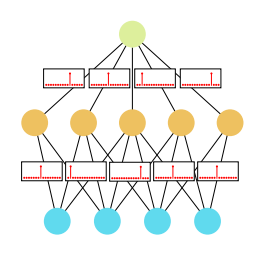
\includegraphics[width=\textwidth]{understandBNN_panel_a_point_estimate.png}
    \caption{Point-estimate NN.}
    \label{fig:nn_point_estimate}
\end{subfigure}\hspace{1.5cm}
\begin{subfigure}[t]{0.36\textwidth}
    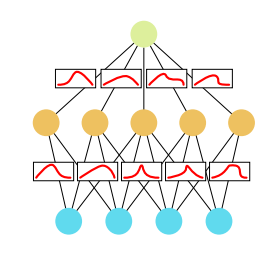
\includegraphics[width=\textwidth]{understandBNN_panel_b_weight_distributions.png}
    \caption{BNN with weight distributions.}
    \label{fig:bnn_weight_distributions}
\end{subfigure}

\caption{Comparison between neural-network formulations. Figure \ref{fig:nn_point_estimate} shows a standard network, in which the weights and biases are fixed after training. Figure \ref{fig:bnn_weight_distributions} shows the Bayesian formulation used in this work, where probability distributions are assigned to the weights and biases. Adapted from \citep{jospin2022bnn}.}
\label{fig:noseno}
\end{figure}

The network itself uses Gaussian priors for the weights and biases and a two-layer architecture with Leaky ReLU activations \citep{maas2013rectifier}. As discussed in Section \ref{sec:bayesian-inference}, MCMC sampling explores the posterior distribution rather than converging to a single point with no uncertainty. The HBNN therefore keeps the flexibility of neural networks while preserving the probabilistic interpretation required for calibrated stellar predictions \citep{jospin2022bnn}.





% for the presentation, also keep in mind that andy always describes these neural neetworks as a sort of one layer, many branches to many layers, many levels of layers, and then they converge to one putput (see fig 1 of 2022). the key is the boceto, to illustrate it. might look for somehting similar, either for resentation itself or for blackboard explanation when in questions



\iffalse

This approach improves results because aggregating predictions from a large ensemble of distinct, independent models generally yields superior predictive accuracy compared to relying on a single deterministic model (galton1907voxpopuli and breiman1996bagging). However, the primary motivation for employing BNNs isn't their enhanced prediction ability, but their rigorous quantification of uncertainty. By evaluating the variance across the multiple sampled models, BNNs provide a mathematically sound measure of prediction confidence, significantly reducing overconfidence compared to classical ANNs (J. Mitros and B. M. Namee, ``On the validity of Bayesian neural networks for uncertainty estimation,'' in AICS, 2019; AND ALSO A. Kristiadi, M. Hein, and P. Hennig, ``Being Bayesian, even just a bit, fixes overconfidence in ReLU networks,'' CoRR, vol. abs/2002.10118, 2020. [Online]. Available: http://arxiv.org/abs/2002.10118). Furthermore, BNNs distinguish between epistemic uncertainty (model uncertainty due to a lack of data) and aleatoric uncertainty (inherent noise within the data itself) (A. D. Kiureghian and O. Ditlevsen, ``Aleatory or epistemic? does it matter?'' Structural Safety, vol. 31, no. 2, pp. 105–112, 2009). This distinction makes BNNs highly data-efficient and less susceptible to overfitting on small datasets (S. Depeweg, J.-M. Hernandez-Lobato, F. Doshi-Velez, and S. Udluft, ``Decomposition of uncertainty in Bayesian deep learning for efficient and risk-sensitive learning,'' in Proceedings of the 35th International Conference on Machine Learning, vol. 80, 2018, pp. 1184–1193).


In this work, we deploy a Hierarchical Bayesian Neural Network (HBNN). A hierarchical (or multilevel) model separates inference into distinct, interconnected levels. In a standard hierarchical structure, the parameters defining a base-level probability distribution are not fixed scalars; rather, they are themselves governed by higher-level probability distributions, known as hyperpriors. In our specific HBNN, the hierarchy distinctly separates the physical modeling of the stellar input parameters from the non-linear regression performed by the network.


Standard errors-in-variables models treat input predictors as independent. Level 1 of the HBNN explicitly models the physical correlations between the measured inputs (e.g., the relationship between effective temperature and surface gravity). So is this just the parameters of the layers and hidden layers?

The true, unobservable physical parameters are treated as latent variables, denoted $x_{\mathrm{latent}}$. To model their interdependencies, $x_{\mathrm{latent}}$ is assigned a zero-mean multivariate normal prior:
\begin{equation}
    x_{\mathrm{latent}} \sim \mathcal{N}(0, \Sigma)
\end{equation}
where $\Sigma$ is the covariance matrix. We utilize an LKJ Cholesky prior (Lewandowski et al., 2009) for the correlation matrix components of $\Sigma$, a standard formulation ensuring the matrix remains mathematically valid. This level links the reported instrumental measurements and their $1\sigma$ errors to the latent variables, calculating a joint probability distribution that accounts for both measurement noise and intrinsic physical correlations. Gaussian distributions are predominantly utilized here and throughout the model due to their computational tractability and ease of generalization to higher dimensions.

In Level 2, the joint probability distribution of $x_{\mathrm{latent}}$ calculated in Level 1 serves as the input to the stochastic neural network, mapping the correlated stellar parameters to the target variable (e.g. stellar mass, $M$). 

Because the network is Bayesian, independent Gaussian priors are placed on all network weights and biases. The architecture utilizes a two-layer structure with a Leaky ReLU activation function, which prevents training from ending too early (bc the gradient vanishes during training). (Maas, A. L., Hannun, A. Y., and Ng, A. Y. (2013). Rectifier nonlinearities improve neural network acoustic models. In Proc. icml (Vol. 30, No. 1, p. 3)). 
Training is executed via Markov Chain Monte Carlo (MCMC) sampling. Rather than utilizing standard gradient descent to converge on a single optimal configuration, MCMC algorithms traverse the high-dimensional parameter space to iteratively sample from the posterior distribution, mathematically generating the required ensemble of stochastic models.

\fi

% Explanation: In deep networks, standard activation functions (like Sigmoid or regular ReLU) can cause the gradients (the math used to update the weights during training) to become $0$. If the gradient is $0$, the network stops learning

% Likelihood is the mathematical probability of observing your exact training data given a specific set of model parameters. It quantifies how accurately a proposed model configuration reproduces the measured target variables.


\subsection{Bayesian Hierarchical Stacking}
The predictions from BART, GP and HBNN are combined through Bayesian Hierarchical Stacking (BHS). Stacking is an ensemble method in which the outputs from several models are combined using learned weights, allowing relevant information from each model to contribute to the final prediction \citep{wolpert1992stacked}. Unlike simple averaging, BHS allows the weights assigned to each level-0 predictor to depend on the input features. This is important because a model may be reliable for near-solar stars but less reliable for more massive objects or for stars with larger uncertainties. The former is the case of the level-0 models used in this work, as described in Section \ref{sec:results}. The final estimate is therefore a locally weighted combination of the three model outputs \citep{yao2022hierarchicalstacking}.

The weights are estimated using cross-validation information, discussed in Section \ref{sec:evaluation}. The hierarchical formulation regularizes the variation in these weights, preventing the stacking model from reacting too strongly to noise in sparsely populated regions of the dataset. Thus, BHS is used as a controlled way to exploit the complementary strengths of the three models while reducing the risk of relying on a single imperfect predictor.


\iffalse

In this context, an individual predictive algorithm or model is referred to as a \textit{generalizer}. By partitioning the training set, training generalizers on one partition, and evaluating them on the other, we can deduce and mathematically correct for the individual biases of each generalizer. Loosely speaking, this strategy combines the generalizers rather than choosing amongst them. This is achieved by taking the output predictions of the base models as input components in a new mathematical space, and then deploying a meta-model to generalize within that new space (David Wolpert. Stacked generalization. Neural Networks, 5:241–259, 12 1992. doi: 10.1016/S0893-6080(05)80023-1).

In our framework, the base generalizers (level-0 models) correspond to our $K=3$ independently fitted probabilistic predictors, each providing a posterior predictive distribution $p_k(y \mid \mathbf{x})$. Our level-0 models are the Bayesian Additive Regression Trees (BART), Gaussian Process (GP), and hierarchical Bayesian neural network (HBNN) discussed previously. A level-1 meta-model is then used to learn how to optimally combine these predictions.


Standard model averaging assigns a fixed, global weight to each model based on overall performance. However, in hierarchical stacking, the weights are not fixed per model; they vary dynamically with the input data. This is crucial because different models can be highly effective at explaining different physical regions of the input space cite yao 2022. Therefore, BHS can be conceptualized as point-wise model averaging.

The stacking weights are estimated by maximizing the leave-one-out (LOO) expected log predictive density, which we approximate using Pareto-smoothed importance sampling (PSIS-LOO) [cite vehtari 2017}]. see Section \ref{sec:evaluation} 

To achieve spatially varying weights across the predictor space, the framework introduces latent, unconstrained variables (logits) (add reference).


Permitting weights to vary freely across the input space risks severe overfitting. To regularize the feature dependence of the weights, we apply a hierarchical prior to the regression coefficients $\beta_k$. Each coefficient vector is modeled as a Gaussian:
\begin{equation}
\beta_{kj} \sim \mathcal{N}(\mu_k, \sigma_k^2), \qquad j = 1, \dots, d,
\label{eq:beta_prior}
\end{equation}
where $d$ is the number of input variables. This hierarchical construction mathematically links the coefficient distributions across the different models. It effectively shrinks $\beta_k$ toward a model-specific mean unless the empirical data provides strong evidence for feature dependence. This balances local adaptation with global regularization.

The use of this two-level architecture is sufficient and robust because the level-1 model does not artificially invent new predictive structures for the target variable; it strictly learns the optimal spatial combination of the probabilistic level-0 predictors. Crucially, uncertainty is rigorously propagated throughout the entire procedure. The epistemic and aleatoric uncertainties inherent to the stellar parameters are captured within the level-0 posteriors $p_k(y \mid \mathbf{x})$, while the uncertainty regarding which model to trust is captured within the posterior of the stacking weights $(\beta_k, \mu_k, \sigma_k)$. In this work, unless stated otherwise, we report final predictions using the posterior mean of $w_k(\mathbf{x}_*)$ evaluated at a new input $\mathbf{x}_*$.

\fi

\subsection{Model Evaluation through Cross-validation} \label{sec:evaluation}
% Data extracted from Rasmussen and Williams (2006).

Model evaluation estimates how well a trained model will generalize to stars that were not used during training. A simple train--validation split gives a direct test of this: part of the dataset is kept aside as a validation subset, and the trained model is then evaluated against it. Nevertheless, the result can depend strongly on the particular partition, since a large validation set reduces the data available for fitting, while a small one gives a noisy estimate of the error \citep{rasmussen2006gpml}.

Cross-validation reduces this dependence on a single split. In $k$-fold cross-validation, the dataset is divided into $k$ subsets; each subset is used once for validation while the remaining subsets are used for training. The reported performance is then averaged over the folds, so every star contributes both to fitting and to out-of-sample assessment \citep{rasmussen2006gpml}. This provides a more stable basis for evaluating the target-variable predictions produced by the models used in this work, allowing for a better comparison between them.

The most exhaustive version is Leave-One-Out Cross-Validation (LOO-CV), where each observation is validated once while the model is trained on all remaining observations. For complex Bayesian models, explicitly refitting the model for every observation is usually too expensive. Therefore, when appropriate, this work uses the efficient LOO approximation proposed by \citet{vehtari2017loo}: Pareto-smoothed importance sampling (PSIS-LOO). This gives a common evaluation criterion without requiring a separate validation set.

\iffalse

To evaluate predictive performance, datasets are traditionally partitioned into distinct training and validation subsets. The model optimizes its parameters on the training set, while the validation set provides an empirical measure of the generalization error, defined as the expected prediction error on unseen, independent data points. 

However, a static train-validation split presents inherent mathematical limitations. Withholding a large fraction of data for validation starves the model of valuable training information, whereas employing a small validation set results in high-variance, unreliable performance estimates (Rasmussen and Williams, 2006). 

To mitigate these drawbacks, $k$-fold cross-validation is employed. This technique partitions the dataset into $k$ disjoint (mutually exclusive) subsets of equal size. In a single iteration, one subset acts as the validation hold-out, while the remaining $k-1$ subsets are aggregated to train the model. This protocol is iterated $k$ times until every subset has served exactly once as the validation set. Consequently, a vast majority of the data is utilized for training in each fold, and every observation is ultimately evaluated as an unseen validation case.

Despite its statistical advantages, standard $k$-fold cross-validation imposes severe computational burdens, as the model must be completely refitted $k$ times. The logical extreme of this method occurs when $k = n$, where $n$ is the total number of observations. This is known as Leave-One-Out Cross-Validation (LOO-CV). While theoretically optimal for performance estimation, standard LOO-CV is computationally intractable for complex Bayesian models, necessitating advanced mathematical approximations (such as Pareto-smoothed importance sampling (PSIS-LOO)) to evaluate the predictive density without requiring explicit refitting (Rasmussen and Williams, 2006).

\fi

\section{Methods} \label{methods}
% A medida que expliques como cada uno de los metodos utiliza las observaicioens directas para calcular parametros, puedes mencionar los papers qu ehayas ido usando. Esto hazlo en el futuro, cuando releas los papers para hacer unos parrafos de explicacion de cada uno de ellos

This section introduces the observational basis of the stellar labels used later to construct the final catalogue. The catalogue is built from three reference methods: detached eclipsing binaries, asteroseismology and interferometry. Spectroscopy is discussed first as context, because it is essential for many stellar parameters, but relies strongly on stellar-atmosphere modelling. This contrast motivates the use of the other three methods as the main sources of high-quality labels, while also making clear that they are not completely free from auxiliary assumptions.

\subsection{Spectroscopy}
%revisar si esta(s) seccion(es) tiene un tono demasiado didactico, lejos de un paper/TFG

%  spectroscopy study the distribution of electromagnetic radiation as a function of wavelength. photometry studies this distribution in large intervals, selected by means of filters, while spectroscopy makes a finer analysis, with higher resolution, by means of optical dispersion devices, such as optical prisms and diffraction gratings. So spectroscopy = wavelength separation
Spectroscopy analyses the stellar radiation received as a function of wavelength. The continuum, discontinuities, absorption lines and molecular bands are produced by physical processes in the stellar atmosphere, and therefore contain information about stellar parameters.

The difficulty is that these quantities are not usually obtained by direct measurement. They are inferred by comparing the observed spectrum with synthetic spectra, line lists and stellar-atmosphere models \citep{tsantaki2018}. Spectroscopy is therefore essential, especially for $T_{\mathrm{eff}}$ and $[\mathrm{Fe}/\mathrm{H}]$, but it can also introduce model-dependent assumptions into any machine-learning model trained on those input features.

%maybe add something about photometry . say that it is very similar or smth. it prolly need atmospheric methods as well. also mention astrometry, which I think doesn't rely on atmopshere, but needs very precise and hard to obtain data, and take too much time to measure. exoplanet transits happen very rarely


\subsection{Eclipsing Binaries}
%add this somewhere, if I find a refernce: DEBs are considered the absolute pinnacle for determining stellar mass and radius.
Detached eclipsing binaries are systems in which two stars orbit each other without significant mass transfer, while their orbital plane causes periodic eclipses as seen from Earth. Because the components are dynamically linked but remain physically separated, they are especially valuable for obtaining fundamental stellar parameters such as $M$ \citep{Southworth2015,Eker2018}.

The measured light curve gives the orbital period, eclipse geometry, relative radii and temperature ratio. Radial-velocity measurements from Doppler shifts then provide the orbital velocities. Combining these observables with Keplerian dynamics yields absolute masses and radii, from which density and surface gravity follow. These quantities are therefore mainly geometric and dynamical.

The atmospheric quantities are less direct. Absolute temperatures and luminosities usually require spectroscopy, colour-temperature relations, parallax, bolometric fluxes, or a combination of these ingredients \citep{Graczyk2022}. For this reason, detached eclipsing binaries are treated as a strong reference source for masses and radii, while their temperature and luminosity labels still require attention to the assumptions used to derive them.

% Revisar que estos dos metodos se cumplan luego en los papers. Puede haber menos, o mas.

\subsection{Asteroseismology}
%revisar si esta(s) seccion(es) tiene un tono demasiado didactico, lejos de un paper/TFG. sobre todo el final sobre los harmonicos

% Rodrigues 2017 explains well this method (especially the used parameters delta nu and nu_max) in its introduction
Asteroseismology studies stellar oscillations. An extensively studied type of oscillations occurs in solar-like stars, where turbulent motion in the outer convective envelope excites pressure waves that propagate through the interior and produce small brightness variations. Time-series photometry and Fourier analysis reveal the characteristic oscillation frequencies of the star \citep{Bellinger2019,Serenelli2021}.

Two global seismic quantities are especially useful. The large frequency separation, $\Delta\nu$, scales with the square root of the mean density, while the frequency of maximum oscillation power, $\nu_{\mathrm{max}}$, is related to surface gravity and effective temperature:
\begin{equation}
\Delta\nu \propto \sqrt{\frac{M}{R^3}}, \qquad
\nu_{\mathrm{max}} \propto \frac{M}{R^2\sqrt{T_{\mathrm{eff}}}} .
\end{equation}
With an external estimate of $T_{\mathrm{eff}}$, these relations constrain mass, radius and $\log g$ \citep{chaplin2013}.

This makes asteroseismology particularly useful for single stars, where direct dynamical masses are usually unavailable. However, the method still depends on scaling relations, external atmospheric inputs and, in more detailed analyses, stellar models. It therefore provides strong constraints, but not completely model-independent labels.

% Asteroseismic $\log g$ values are far more precise than any other method for single stars. (add reference

\subsection{Interferometry}
Interferometry combines the light collected by separated telescopes, effectively increasing the angular resolution beyond that of a single aperture. For nearby bright stars, this makes it possible to measure the angular diameter. Together with an independent distance, usually from parallax, the stellar radius can then be obtained geometrically \citep{ligi2016}.

If the bolometric flux is also known, the effective temperature follows from the Stefan--Boltzmann relation. This makes interferometry one of the most empirical routes to stellar radii and temperatures, and it is used in benchmark-star calibrations \citep{Soubiran2024}. The method is not fully assumption-free, because bolometric flux estimates require extinction corrections and model-dependent treatment of unobserved spectral regions. It is also limited to stars with sufficiently large angular diameters, so its contribution to the total sample is small.

\subsection{Limits of Model Independence}
MIGHT REMOVE THIS SECTION. NOT BECAUSE OF SPACE; BUT AVOIDING UNNCESSARY REPETITION

The methods described above are used because they reduce the dependence on stellar-atmosphere models, but they do not remove modelling assumptions completely. Eclipsing binaries still require external calibrations for absolute temperatures and luminosities, asteroseismic masses and radii depend on scaling relations and an external $T_{\mathrm{eff}}$ estimate, and interferometric temperatures require bolometric fluxes and extinction corrections.

For this reason, the catalogues used in this work should not be interpreted as perfectly model-independent ground truth. They are instead high-quality reference labels, selected because their central constraints are closer to geometry or dynamics than to atmospheric modelling: eclipsing binaries provide strong masses and radii, asteroseismology constrains stellar density and surface gravity, and interferometry gives empirical radii and temperatures for suitable nearby stars. This compromise is important for the machine-learning models trained later, since their predictions cannot be more physically reliable than the labels from which they learn.


\section{Data} \label{sec:data}
% This paper talks about prioritising Data instead of models. Not prioritising good data over a large quantity of data. It explicitly says it wants high quality and quantity of data. Might use it in the future, tho. https://www.semanticscholar.org/paper/Data-centric-Artificial-Intelligence%3A-A-Survey-Zha-Bhat/12c6be503e4e5b7c9cb1810152d4364f26628a8d Zha et al., 2023

In supervised machine learning, the quality of the input features can be as important as the size of the training set. Large catalogues affected by heterogeneous systematics may lead the models to reproduce those biases instead of learning the underlying physical relations \citep{li2021dataquality}. For this reason, this work follows a quality-centred strategy, prioritising a smaller, traceable and physically reliable calibration set over a larger but less controlled sample.

Following the guidance of \citet{moya2018}, whose catalogue covered approximately the mass range $0.7\,M_\odot < M < 2.5\,M_\odot$, an extended stellar catalogue was assembled from literature sources with complementary parameter coverage. The lower boundary has been reduced to $0.5\,M_\odot$, since one of the aims of this extension was to improve the coverage at lower masses. Such reference stars are needed to calibrate predictions for M-type stars, which are especially relevant in exoplanet studies (see Section \ref{subsec:dataset_b}). The aim was to obtain a statistically meaningful and heterogeneous sample, while preserving clear information on the uncertainties of the stellar parameters. Because the reported uncertainties are propagated into the final mass predictions in the probabilistic models in this work, this uncertainty-treatment is a key aspect.

As explained in Section \ref{methods}, the reference sources were selected according to three observational methods: eclipsing binaries, asteroseismology and interferometry. Studies published between 2018 and 2025 were reviewed when they provided uncertainties and as many of the required stellar parameters as possible, listed in Table \ref{MS_catalog_database_D}. Stellar mass and radius were mandatory, since stellar densities were computed from them. This initial compilation contained 16094 stars before duplicate removal and quality cleaning.

\begin{table}[H]
\centering
\setlength{\tabcolsep}{4pt}
\caption{Summary of the stellar parameters contributed by each catalogue to the final calibration sample of 767 usable main-sequence stars. Each value gives the number of stars with the corresponding available parameter. The metallicity column combines $[\mathrm{Fe}/\mathrm{H}]$ and $[\mathrm{M}/\mathrm{H}]$. Catalogues not individually discussed in this work are described in \citet{moya2018}.}
\footnotesize
\begin{tabular}{lrrrrrrrr}
\hline\hline
Catalogue & $M$ & $R$ & $T_{\mathrm{eff}}$ & $L$ & Meta & $\log g$ & $\rho$ & $a$\\
~ & ($M_\odot$) & ($R_\odot$) & (K) & ($L_\odot$) & (dex) & (dex) & ($\rho_\odot$) & ($R_\odot$)\\
\hline
Serenelli et al. (2017) & 240 & 240 & 240 & 240 & 240 & 240 & 240 & 0\\
Xiong et al. (2023) & 141 & 141 & 141 & 141 & 141 & 141 & 141 & 141\\
Chaplin et al. (2014, SDSS) & 62 & 62 & 62 & 62 & 62 & 62 & 62 & 0\\
Eker et al. (2014) & 54 & 54 & 54 & 54 & 54 & 54 & 54 & 54\\
Yildiz et al. (2019) & 42 & 42 & 42 & 42 & 42 & 42 & 42 & 0\\
Lund et al. (2016) & 28 & 28 & 28 & 28 & 28 & 28 & 28 & 0\\
Huber et al. (2013) & 24 & 24 & 24 & 24 & 24 & 0 & 24 & 0\\
Silva Aguirre et al. (2015) & 24 & 24 & 24 & 24 & 24 & 24 & 24 & 0\\
Wang et al. (2025) & 20 & 20 & 20 & 20 & 20 & 20 & 20 & 20\\
Eker et al. (2014, 2018) & 17 & 17 & 17 & 17 & 17 & 17 & 17 & 17\\
Silva Aguirre et al. (2017) & 15 & 15 & 15 & 15 & 15 & 15 & 15 & 0\\
Soubiran et al. (2024) & 13 & 13 & 13 & 13 & 13 & 13 & 13 & 0\\
Helminiak et al. (2019) & 11 & 11 & 11 & 11 & 11 & 11 & 11 & 11\\
Pan et al. (2025) & 10 & 10 & 10 & 10 & 10 & 10 & 10 & 10\\
Ligi et al. (2016) & 10 & 10 & 10 & 10 & 10 & 0 & 10 & 0\\
Chaplin et al. (2014, Bruntt) & 8 & 8 & 8 & 8 & 8 & 8 & 8 & 0\\
Özdarcan et al. (2025, Feb.) & 7 & 7 & 7 & 7 & 7 & 7 & 7 & 7\\
Malkov et al. (2007) & 4 & 4 & 4 & 4 & 4 & 0 & 4 & 0\\
Welsh et al. (2012) & 4 & 4 & 4 & 4 & 4 & 4 & 4 & 4\\
Brogaard et al. (2018) & 3 & 3 & 3 & 3 & 3 & 3 & 3 & 3\\
Özdarcan et al. (2024) & 3 & 3 & 3 & 3 & 3 & 3 & 3 & 3\\
Torres et al. (2010) & 3 & 3 & 3 & 3 & 3 & 3 & 3 & 3\\
Çakırlı et al. (2025, Apr.) & 2 & 2 & 2 & 2 & 2 & 2 & 2 & 2\\
Çakırlı et al. (2025, Dec.) & 2 & 2 & 2 & 2 & 2 & 2 & 2 & 2\\
Knudstrup et al. (2020) & 2 & 2 & 2 & 2 & 2 & 2 & 2 & 2\\
Martin et al. (2024, Dec.) & 2 & 2 & 2 & 2 & 2 & 2 & 2 & 2\\
Miller et al. (2022) & 2 & 2 & 2 & 2 & 2 & 2 & 2 & 2\\
Miller et al. (2026) & 2 & 2 & 2 & 2 & 2 & 2 & 2 & 2\\
O'Brien et al. (2025) & 2 & 2 & 2 & 2 & 2 & 2 & 2 & 2\\
Xu et al. (2026) & 2 & 2 & 2 & 2 & 2 & 2 & 2 & 2\\
Yücel et al. (2026) & 2 & 2 & 2 & 2 & 2 & 2 & 2 & 2\\
Bond et al. (2020) & 1 & 1 & 1 & 1 & 1 & 1 & 1 & 1\\
Jennings et al. (2024) & 1 & 1 & 1 & 1 & 1 & 1 & 1 & 0\\
Lund et al. (2019) & 1 & 1 & 1 & 1 & 1 & 1 & 1 & 0\\
Maxted et al. (2023) & 1 & 1 & 1 & 1 & 1 & 1 & 1 & 1\\
Maxted et al. (2025) & 1 & 1 & 1 & 1 & 1 & 1 & 1 & 1\\
Thomsen et al. (2022) & 1 & 1 & 1 & 1 & 1 & 1 & 1 & 1\\
Total & 767 & 767 & 767 & 767 & 767 & 729 & 767 & 295\\
\hline
\end{tabular}
\label{MS_catalog_database_D}
\end{table}

\subsection{Catalogues}
The literature sources used to compile the catalogue are summarised in Table \ref{tab:catalogue_sources}. The main role of each source in the construction of the final sample, is also indicated, since not all catalogues contributed the same type of information.

\begin{table}[H]
\centering
\caption{Summary of the main literature sources used to build the stellar catalogue. The initial-entries column gives the number of main-sequence stars taken from each source before duplicate removal and further quality cleaning (see Section \ref{sec:cleaning}). The method column indicates the main observational basis of each source, while the final column summarises its role in the catalogue construction and any relevant technical treatment applied during the merging process.}
\label{tab:catalogue_sources}
\scriptsize
\setlength{\tabcolsep}{3pt}
\renewcommand{\arraystretch}{1.12}
\begin{tabular}{p{0.17\linewidth}p{0.09\linewidth}p{0.18\linewidth}p{0.22\linewidth}p{0.27\linewidth}}
\hline\hline
Source & Initial entries & Main method & Main contribution & Notes for this work \\
\hline
\citet{Eker2018} & 508 & Detached eclipsing binaries & Accurate stellar parameters for main-sequence binary components over a broad mass range & Used as a high-quality reference for masses and radii; also relevant for calibrating $L$ and $T_{\mathrm{eff}}$. \\
\hline
\citet{Helminiak2019} & 22 & Detached eclipsing binaries with spectroscopic support & Binary-star parameters with additional atmospheric information & Treated with care because the reported abundance information was given as $[\alpha/\mathrm{Fe}]$, not directly in the metallicity scale adopted here. \\
\hline
\citet{Graczyk2021,Graczyk2022} & 28 & Detached eclipsing binaries & Surface-brightness--colour calibration samples & The dwarf-star calibrating sample of \citet{Graczyk2022} was adopted as a strong reference source. \\
\hline
\citet{Nsamba2025} & 8 & Benchmark stars & Pre-existing benchmark-star compilation & Required careful duplicate removal because of overlap with other catalogues. \\
\hline
\citet{Bellinger2019} & 97 & Asteroseismology & Asteroseismic masses and radii for mostly solar-like stars & Several objects lacked some atmospheric parameters required in this work. \\
\hline
\citet{Serenelli2021} & 106 & Mixed benchmark compilation & Stellar mass-determination methods across the HR diagram, including eclipsing binaries and asteroseismology & Contributed a large number of reliable stars, although luminosity and metallicity were not always available. \\
\hline
\citet{Soubiran2024} & 31 & Interferometry and benchmark-star calibration & Gaia FGK benchmark stars with fundamental $T_{\mathrm{eff}}$ and $\log g$ & Luminosities were provided as $\log L$, requiring conversion before use in the catalogue. \\
\hline
\citet{Xiong2023} & 354 & Eclipsing binaries with spectroscopic information & Empirical library based on binary-star parameters & Treated with additional caution because of non-standard identifiers and some comparatively large uncertainties. \\
\hline
\citet{Sayeed2025} & 694 & Asteroseismology & Homogeneous catalogue of Kepler main-sequence and subgiant solar-like oscillators & Metallicity was not always accompanied by uncertainty. \\
\hline
\citet{Yildiz2019} & 74 & Asteroseismology & Masses and radii for Kepler and CoRoT solar-like oscillators & Metallicities reported as surface metal mass fractions were converted to the logarithmic scale. \\
\hline
\end{tabular}
\end{table}


\citet{Yildiz2019} provided metallicities as surface metal mass fractions $Z_s$. They were converted to the logarithmic scale using $[\mathrm{M}/\mathrm{H}] = \log \left[(Z_s/X_s)/(Z/X)_\odot\right]$, adopting $X_s \simeq 0.7381$ and $(Z/X)_\odot = 0.0181$ from \citet{asplund2009}.


% \citet{Southworth2015} is the famous DEBCat, but it didn't finally make the sample because L was computed from model-dependet methods

\subsection{Cleaning} \label{sec:cleaning}
When the same star appeared in several catalogues, the retained entry was chosen according to the reliability of the source. Priority was given to catalogues providing the most direct stellar parameters, smaller reported uncertainties and a more complete set of parameters. Regularly updated catalogues and benchmark-star compilations were also preferred over more heterogeneous or less traceable sources. This meant favouring high-precision eclipsing-binary catalogues such as \citet{Eker2018} and the calibrating samples of \citet{Graczyk2022}, benchmark compilations such as the Gaia FGK benchmark-star catalogue \citep{Soubiran2024}, and samples cross-validated across different methods, such as those in \citet{Serenelli2021}. After duplicate removal, 13783 stars remained.

The cleaned sample was then restricted to main-sequence candidates using a criterion based on $\log g$. Following \citet{bilir2008}, stars with $\log g > 4.0$ were classified as main-sequence objects, except for extremely large values of $\log g$ ($\gtrsim 5.5$), which were not interpreted as normal main-sequence stars. Although this threshold is approximate, the effect of applying different classification criteria was already analysed by \citet{moya2018}. They found that the choice between a simple threshold and a more robust classification method had little influence on the final results. The $\log g$ criterion adopted here was therefore considered sufficient for the purposes of this work.

1915 stars remained after this selection, although not all of them contained every required parameter. In principle, incomplete entries could be retained in a Bayesian framework by treating missing quantities as latent variables, provided that an explicit model for the missing-data process is specified \citep[p.~511]{mcelreath2020}. In this work, however, parameter completeness and direct traceability were prioritised, so this kind of imputation was not used. % IDK what latent means here

% \begin{table}[H]
% \centering
% \caption{Secondary sources used to complement missing stellar parameters. During the catalogue merging process, when a preferred primary source (Output catalogue) lacked data for specific parameters, the gaps were filled using the secondary catalogues listed in the corresponding columns.}
% \begin{tabular}{c}
% Ejemplo tabla que tarda poco en compilar\\
% \end{tabular}
% \label{Tab:secondary sources}
% \end{table}

The newly compiled 1915-star sample was then cross-matched with the catalogue of \citet{moya2018} in order to merge both sources, while avoiding duplicates and retaining only the highest-quality entries. Following the same data-centred strategy, stars were removed when they had excessively large uncertainties, zero reported uncertainty in any parameter except $a$, were not classified as main-sequence stars in both catalogues, or had duplicated identifiers. This reduced the sample to 784 stars. Section \ref{subsec:dataset_a} explains the later removal of 17 additional objects, leading to the final training sample of $n=767$ stars.

Although each star in the final merged sample is assigned a primary catalogue identifier according to the reliability criteria described above, the individual stellar parameters for a given entry do not always originate from that single source. To maximise completeness, the merging algorithm constructed composite entries: when the primary catalogue lacked a given parameter, the missing value was filled from an available secondary catalogue. The final parameter set for a star can therefore be heterogeneous in origin. To preserve traceability, a more detailed internal provenance table was used alongside Table \ref{MS_catalog_database_D}; for each primary source, it records which secondary catalogues were queried to fill each missing parameter. When several secondary sources were available, they were prioritised according to the reliability hierarchy described above.

The Hertzsprung--Russell diagram was used as a final consistency check for the cleaned sample. This diagram relates stellar luminosity to effective temperature and is commonly used to identify evolutionary stages, especially the main sequence. As shown in Figure \ref{fig:HRdiagram}, the stars mostly follow the expected main-sequence behaviour, with luminosity decreasing towards lower effective temperatures. FGK stars occupy approximately $T_{\mathrm{eff}} \sim 3500$--$7400\,\mathrm{K}$ \citep{pecaut2013}, or $\log_{10}T_{\mathrm{eff}} \sim 3.54$--$3.87$. Most of the sample lies in this regime, especially the asteroseismic and interferometric stars. The eclipsing-binary subsample is also mainly concentrated around the main sequence, but it spans a broader region of the diagram.

\begin{figure}[H]
    \centering
    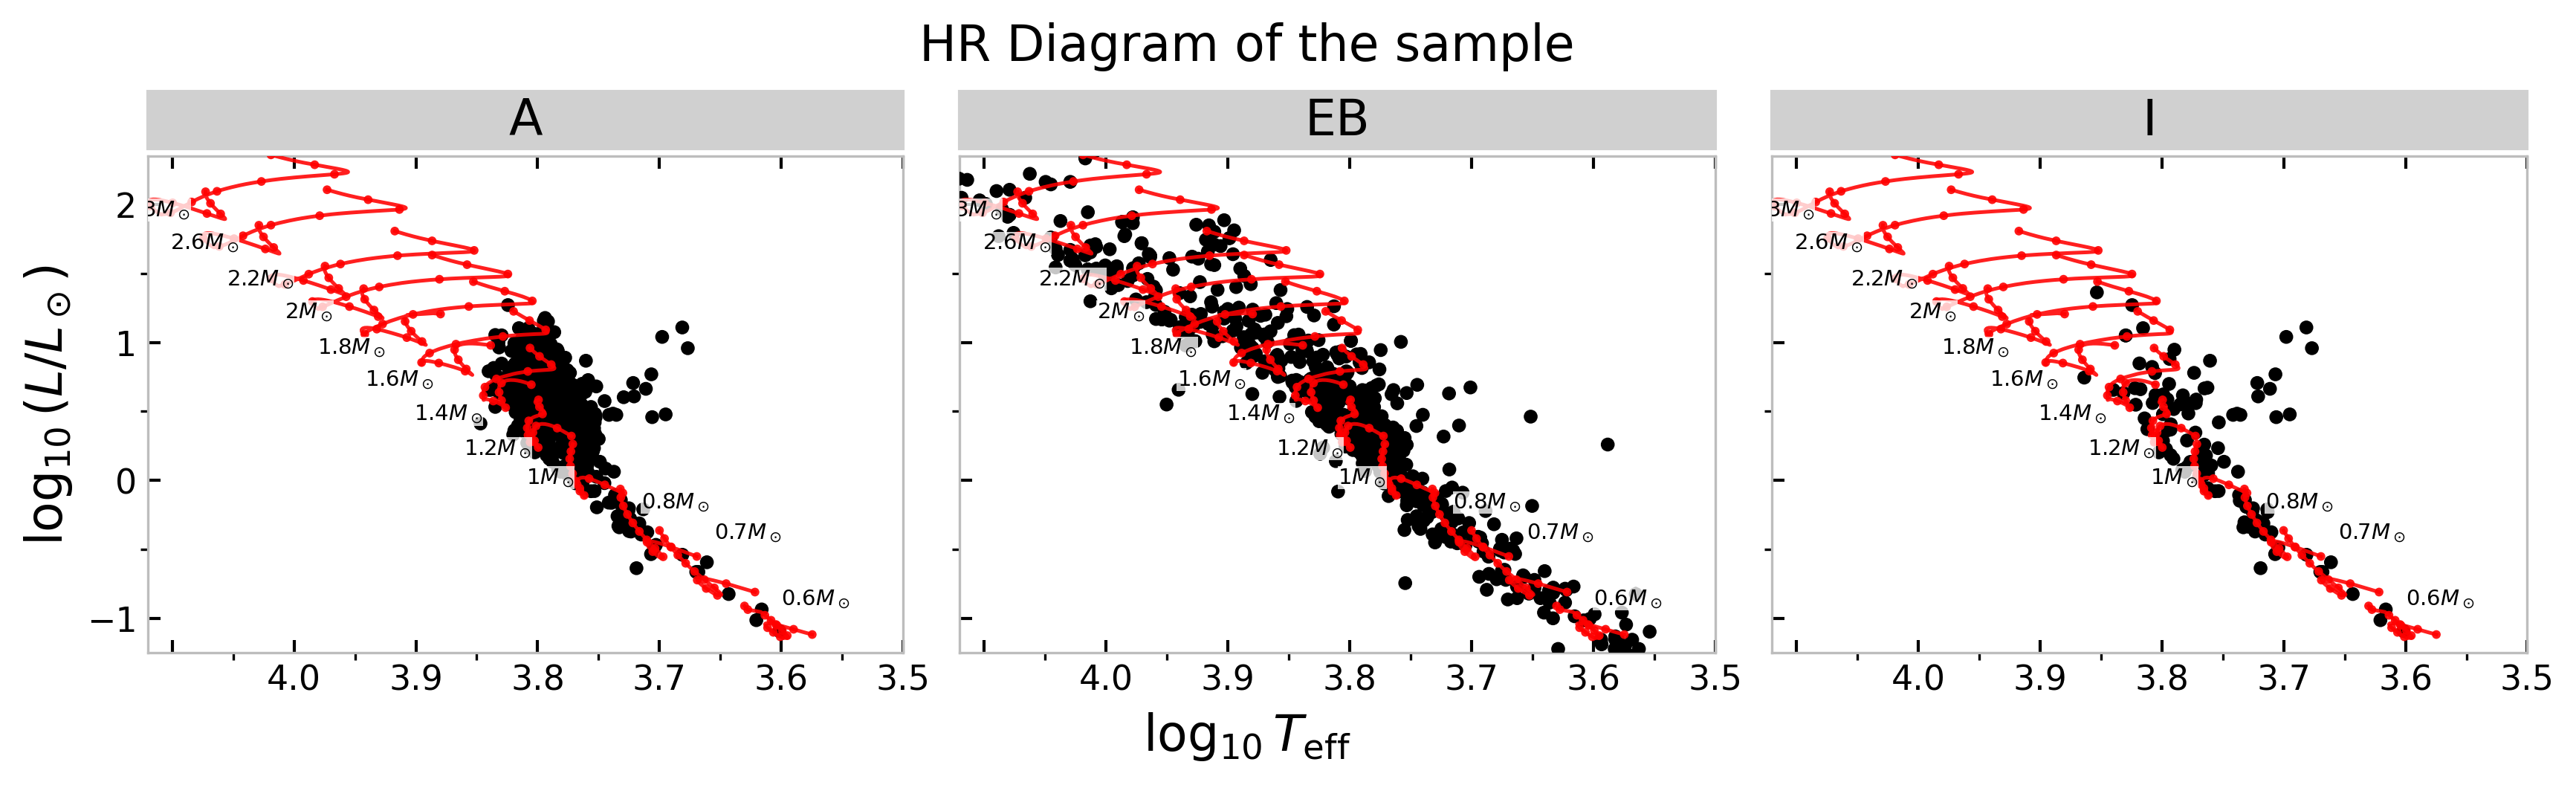
\includegraphics[width=0.99\linewidth]{hr_diagram_parsec_sample_clean.png}
    \caption{HR diagram of the 767 stars in the final sample. The red curves are theoretical evolutionary tracks of different masses obtained with PARSEC \citep{bressan2012}. The sample is divided by the main method used to study each star: asteroseismology, eclipsing binaries and interferometry.}
    \label{fig:HRdiagram}
\end{figure}

Finally, Section \ref{sec:dataset_C} requires the computation of oblateness (Equation \ref{eq:oblateness}), which depends on the orbital semi-major axis $a$. This parameter was often reported without an uncertainty. To retain a statistically meaningful sample, the missing uncertainty was estimated from four significant digits of the reported value. This produced 295 stars with computed oblateness, 48 of which used this uncertainty estimate.



\section{Machine Learning Model Training} \label{sec:results}
The behaviours and quantitative results described in these sections were consistent across different random-seed runs for the four analysed models, keeping the same inputs, target and training strategy. The main evaluation metrics are the Mean Absolute Error (MAE), which measures the average absolute difference between the true masses $m_i$ and the model estimates $\hat{m}_i$; the Mean Absolute Relative Difference (MARD), which measures the average relative accuracy across $N$ samples; and the Mean Relative Difference (MRD), which measures the signed relative bias of the predictions with respect to the true values.

\begin{equation}
\text{MAE} = \frac{\sum_{i=1}^N |m_i - \hat{m}_i|}{N}, \quad \text{MARD} = \frac{\sum_{i=1}^N \frac{|m_i - \hat{m}_i|}{m_i}}{N}, \quad \text{MRD} = \frac{\sum_{i=1}^N \frac{m_i - \hat{m}_i}{m_i}}{N}.
\end{equation}

\subsection{Mass Predictions for FGK-type Stars} \label{subsec:dataset_a}
Main-sequence stars of spectral types F, G and K are especially useful in stellar studies because they are common survey targets and therefore often have well-measured atmospheric parameters. By contrast, main-sequence M-type stars are less extensively documented. They are cooler, low-mass objects that burn hydrogen slowly and evolve very little over the age of the Universe \citep{laughlin1997}. Their intrinsic faintness and slow evolution make precise stellar parameters difficult to obtain \citep{chabrier2000}.

\citet{maxted2023benchmark} proposed a way to obtain information about M-type stars by studying eclipsing-binary systems in which the M star is the secondary component of a better-characterized primary star. Because many eclipsing-binary parameters are measured relative to the two components, information about one star can help constrain the other \citep{Southworth2015}. This motivates a focus on systems with an FGK-type primary and an M-type secondary: accurate mass predictions for the better-characterized FGK component can improve the inferred properties of the lower-mass companion. This helps to extend the calibration towards the M-star regime, where high-quality masses remain scarce.

As discussed in Section \ref{sec:cleaning}, Figure \ref{fig:HRdiagram} shows that the catalogue compiled in this work is rich in FGK-type stars, making this first mass-prediction experiment well suited to the available data. Following \citet{moya2018}, $T_{\mathrm{eff}}$, $\rho$ and $[\mathrm{Fe}/\mathrm{H}]$ were adopted as input parameters for stellar-mass estimation. This choice is motivated by well-studied eclipsing binaries, for which these quantities can be obtained more precisely than alternatives such as $\log g$ or $L$. After combining the stars compiled in this work with the Moya catalogue, applying the main-sequence selection described in Section \ref{sec:data}, requiring these three input parameters, and removing stars with zero reported uncertainty, the final available set contained 767 stars. Of these, 618 were used for training and the remaining 155 stars, corresponding to $20\%$, were retained as a holdout set for testing. The holdout set was repeatedly randomly selected for each seed run.

\subsubsection*{Results}

The behaviour described in this section was consistent across different random-seed runs for the four analysed models. The main evaluation metrics are the Mean Absolute Error (MAE), which measures the average absolute difference between the true masses $m_i$ and the model estimates $\hat{m}_i$; the Mean Absolute Relative Difference (MARD), which measures the average relative accuracy across $N$ samples; and the Mean Relative Difference (MRD), which measures the signed relative bias of the predictions with respect to the true values.

\begin{equation}
\text{MAE} = \frac{\sum_{i=1}^N |m_i - \hat{m}_i|}{N}, \quad \text{MARD} = \frac{\sum_{i=1}^N \frac{|m_i - \hat{m}_i|}{m_i}}{N}, \quad \text{MRD} = \frac{\sum_{i=1}^N \frac{m_i - \hat{m}_i}{m_i}}{N}.
\end{equation}

Figure \ref{fig:hbnn_mass_predictions} shows the HBNN mass predictions for one representative run. In the prediction panel, the points mostly follow the 1:1 relation between predicted and true mass. However, the distribution is not completely uniform: lower-mass stars tend to be overpredicted, whereas higher-mass stars tend to be underpredicted. When averaged over the full holdout set, these two effects partly cancel, leading to a Mean Relative Difference close to zero, $0.71\%$, as shown in Table \ref{tab:model_mard_mrd}.

This trend is more clearly visible in the residual plot\footnote{For visual clarity, residuals were defined as $M_{\mathrm{pred}}-M_{\mathrm{true}}$ in the figures, including \ref{fig:mass_holdout_all_models}, while in the MAE, MARD and MRD definitions the sign is switched, $M_{\mathrm{true}}-M_{\mathrm{pred}}$.}, Figure \ref{fig:hbnn_mass_residuals}. The residuals change sign at approximately $1.3\,M_\odot$: lower-mass stars tend to have positive residuals, while higher-mass stars tend to have negative residuals. Thus, HBNN performs well for the main, near-solar-mass population, where most predictions agree with $M_{\mathrm{true}}$ within $1\sigma$. The model should, however, be treated with caution outside this central region, especially for higher masses.

\begin{figure}[H]
\centering
\captionsetup[subfigure]{font=small}

% Top row: HBNN, GP
\begin{subfigure}[t]{0.24\textwidth}
    \centering
    
\includegraphics[width=\linewidth]{HBNN_mass_3param_L_1000_seed_225_full_prediction.png}
    \caption{HBNN prediction.}
    \label{fig:hbnn_mass_predictions}
\end{subfigure}
\hfill
\begin{subfigure}[t]{0.24\textwidth}
    \centering
    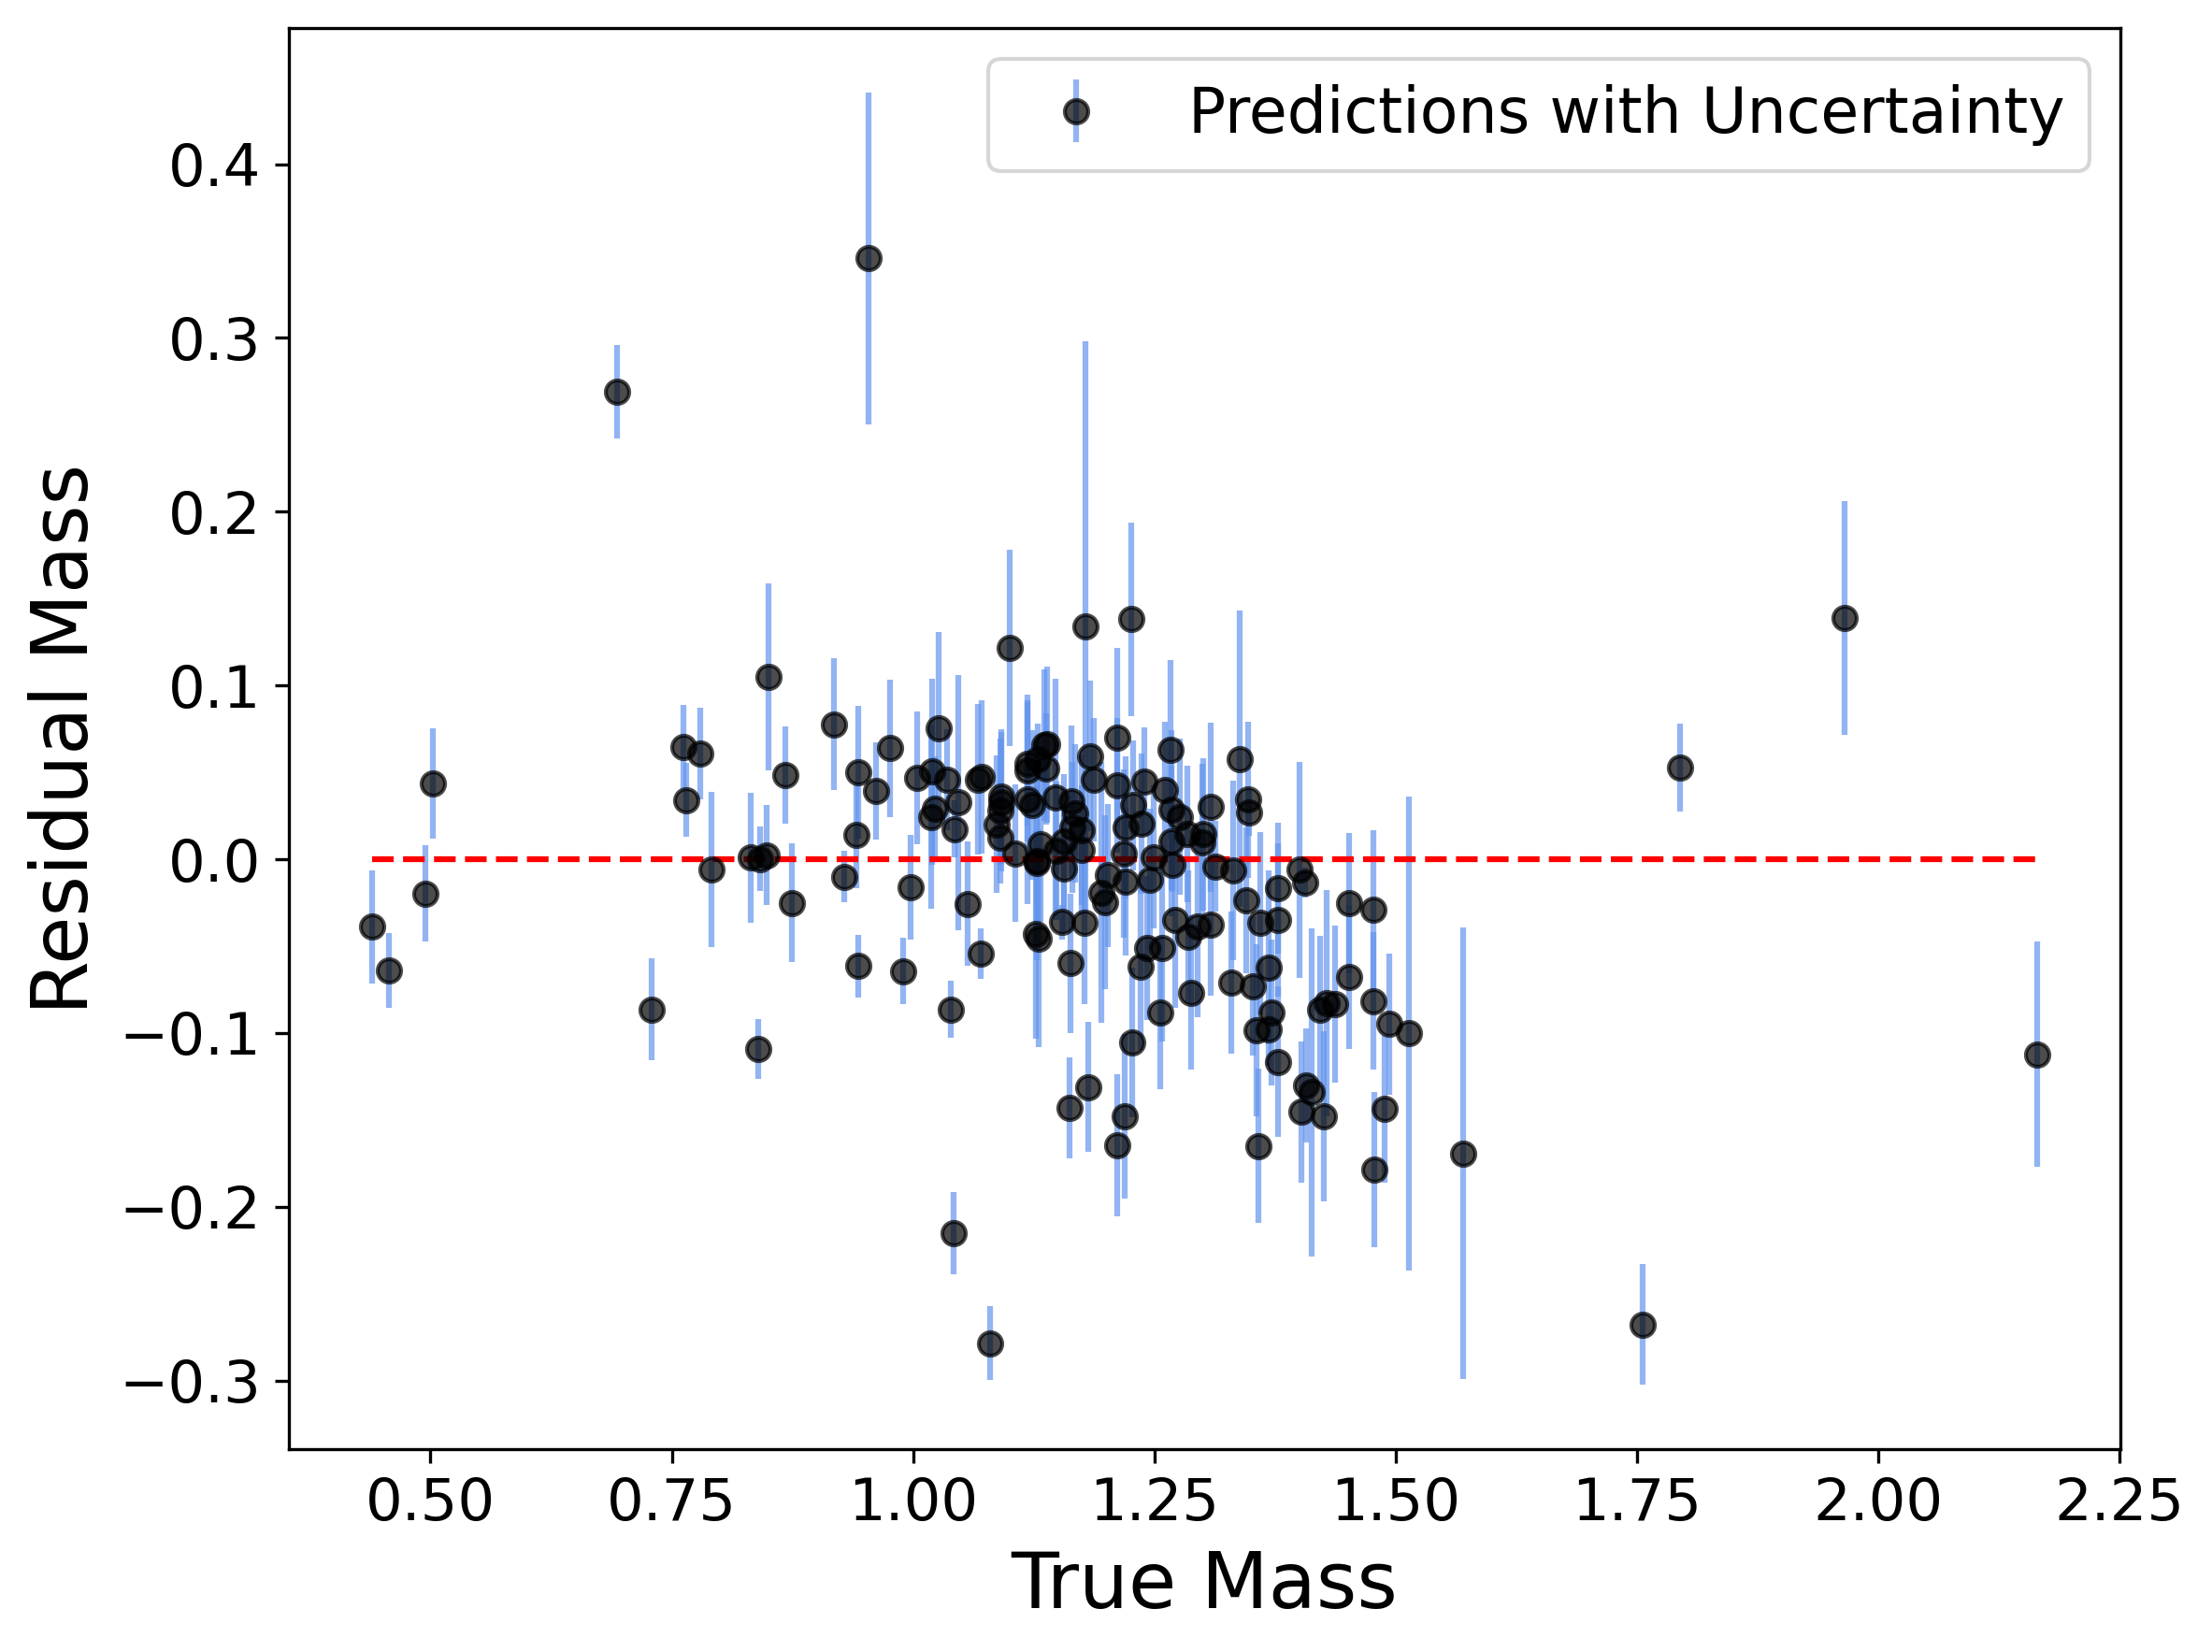
\includegraphics[width=\linewidth]{HBNN_mass_3param_L_1000_seed_225_full_residual.png}
    \caption{HBNN residuals.}
    \label{fig:hbnn_mass_residuals}
\end{subfigure}
\hfill
\begin{subfigure}[t]{0.24\textwidth}
    \centering
    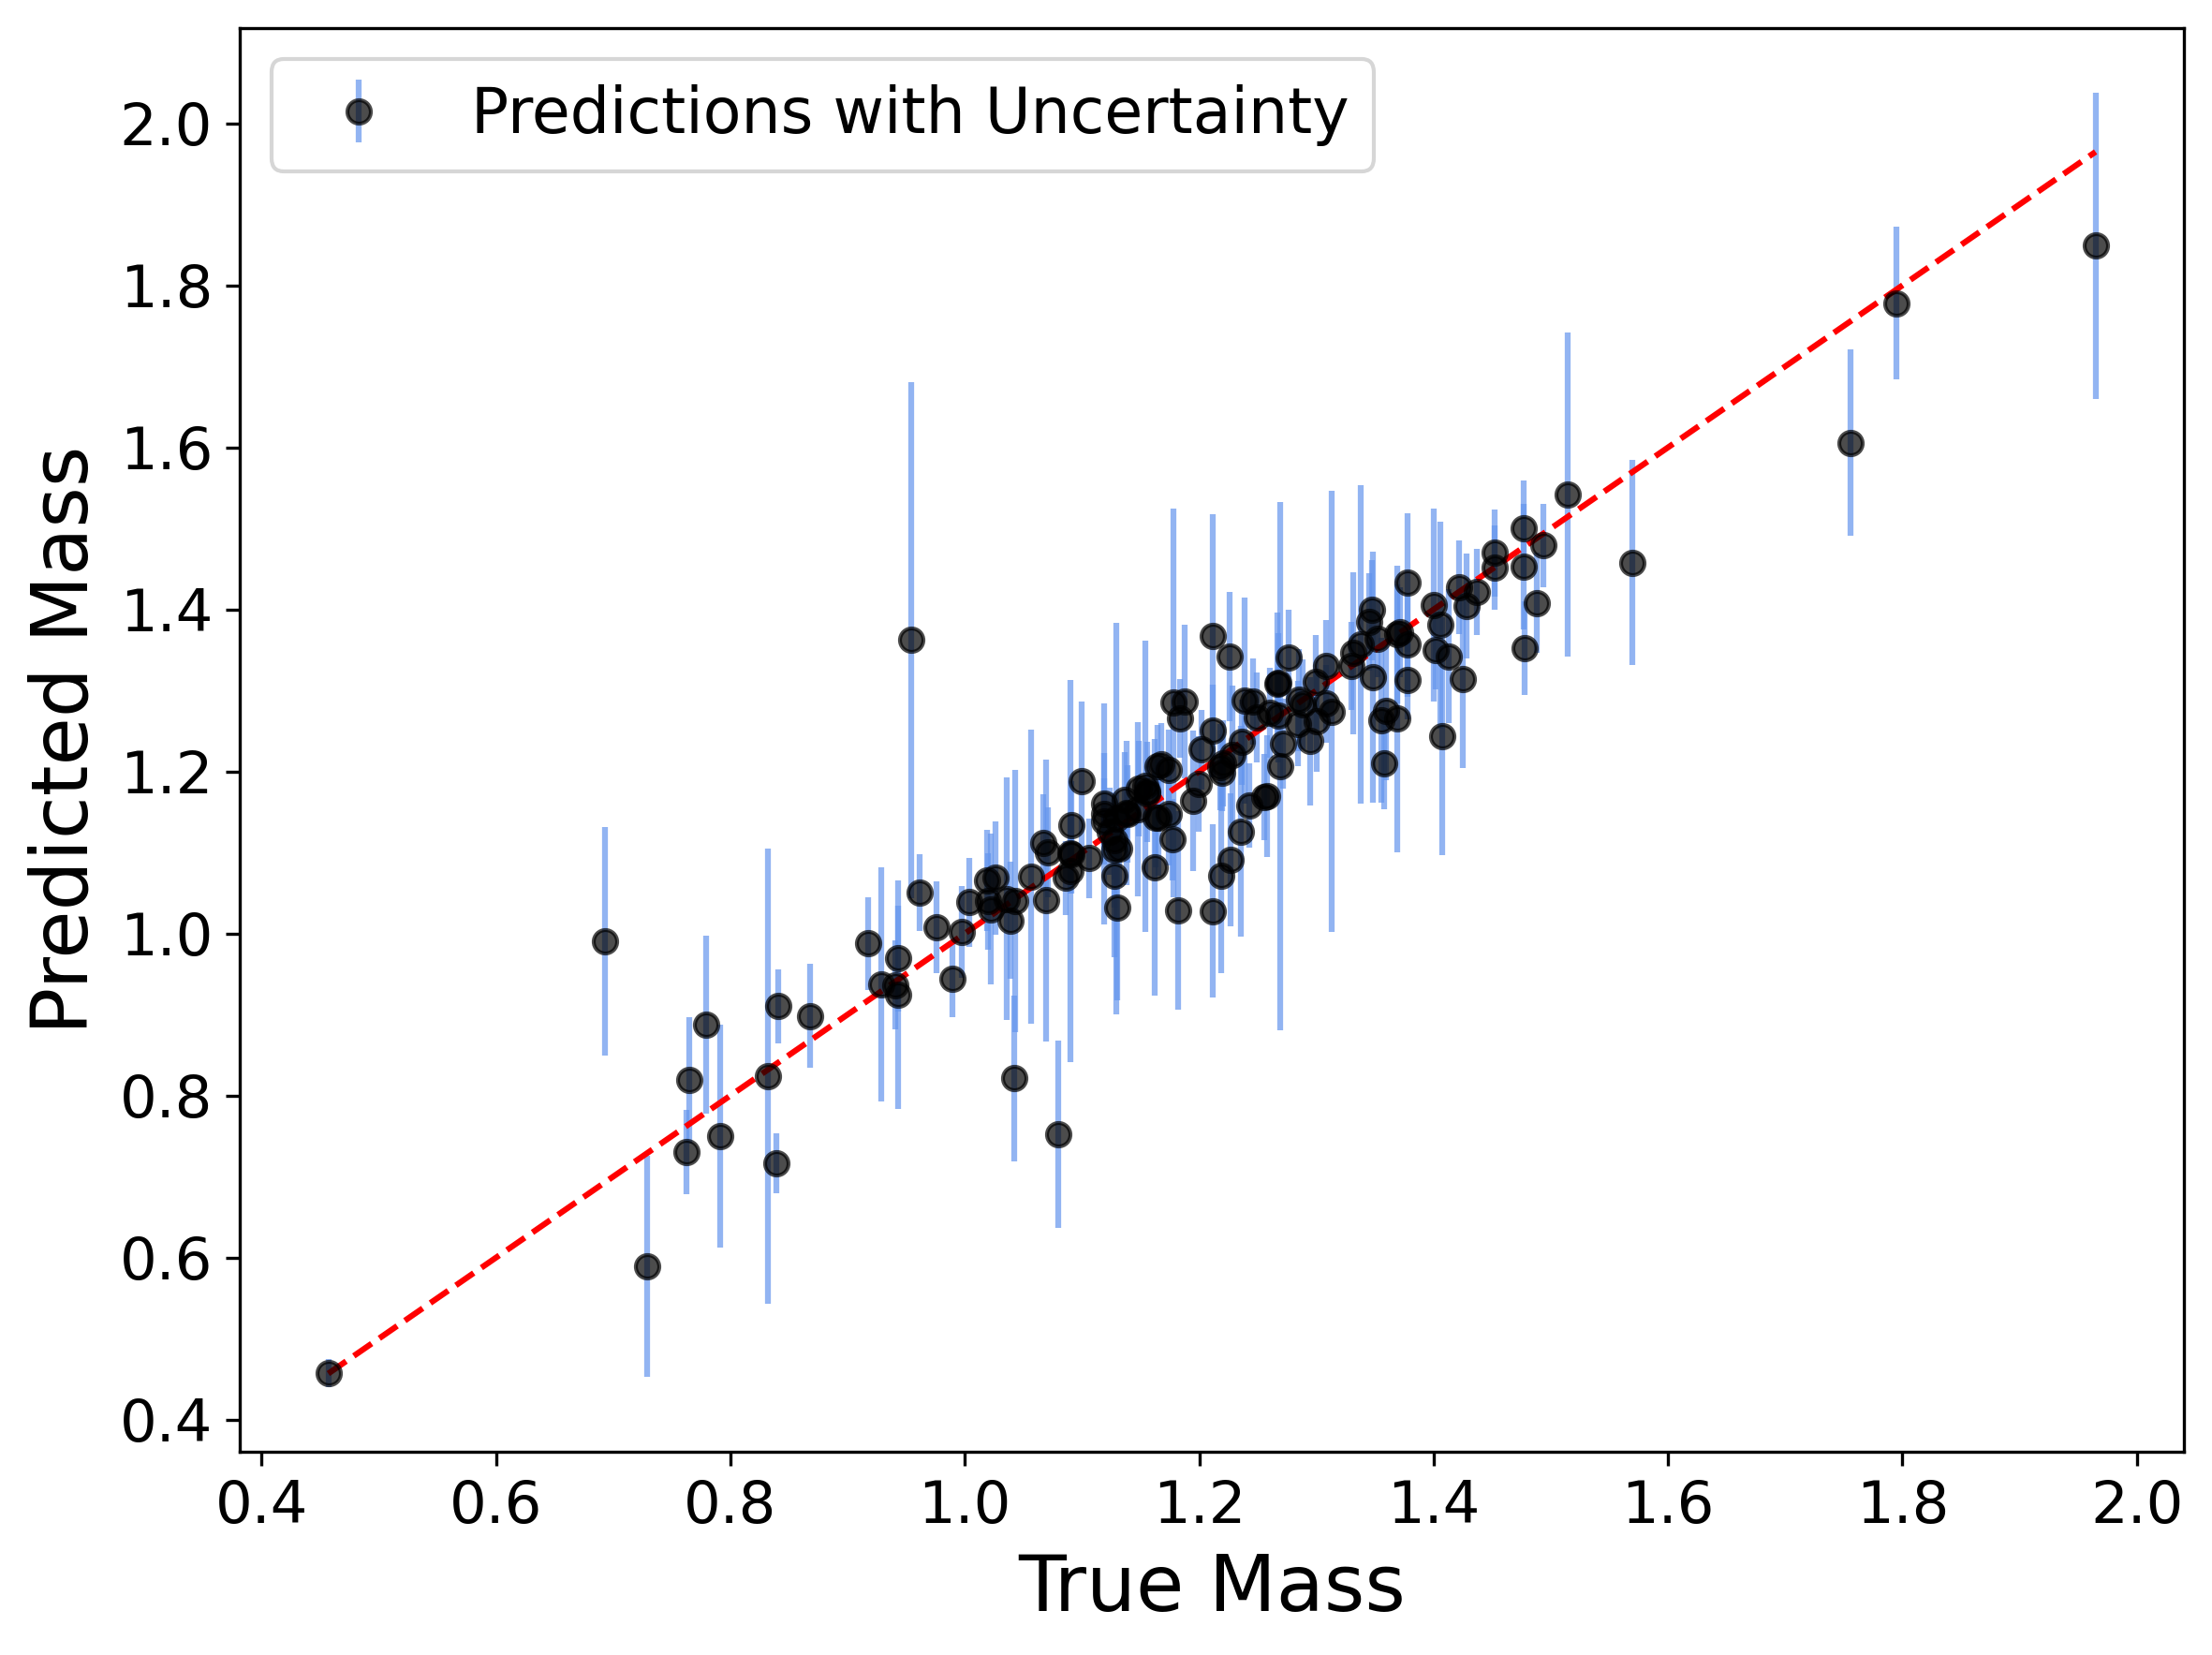
\includegraphics[width=\linewidth]{GP_mass_3param_L_1000_seed_225_filtered_95_prediction.png}
    \caption{GP prediction.}
    \label{fig:gp_mass_predictions}
\end{subfigure}
\hfill
\begin{subfigure}[t]{0.24\textwidth}
    \centering
    
\includegraphics[width=\linewidth]{GP_mass_3param_L_1000_seed_225_filtered_95_residual.png}
    \caption{GP residuals.}
    \label{fig:gp_mass_residuals}
\end{subfigure}

\vspace{0.4cm}

% Bottom row: BART, BHS
\begin{subfigure}[t]{0.24\textwidth}
    \centering
    
\includegraphics[width=\linewidth]{BART_mass_3param_L_prediction_seed_225_full_prediction.png}
    \caption{BART prediction.}
    \label{fig:bart_mass_predictions}
\end{subfigure}
\hfill
\begin{subfigure}[t]{0.24\textwidth}
    \centering
    
\includegraphics[width=\linewidth]{BART_mass_3param_L_prediction_seed_225_full_residual.png}
    \caption{BART residuals.}
    \label{fig:bart_mass_residuals}
\end{subfigure}
\hfill
\begin{subfigure}[t]{0.24\textwidth}
    \centering
    
\includegraphics[width=\linewidth]{BHS_mass_3param_L_prediction_seed_225_filtered_95_prediction.png}
    \caption{BHS prediction.}
    \label{fig:bhs_mass_predictions}
\end{subfigure}
\hfill
\begin{subfigure}[t]{0.24\textwidth}
    \centering
    
\includegraphics[width=\linewidth]{BHS_mass_3param_L_prediction_seed_225_filtered_95_residual.png}
    \caption{BHS residuals.}
    \label{fig:bhs_mass_residuals}
\end{subfigure}

\caption{Holdout-test performance of the HBNN, GP, BART and BHS mass models trained with $T_{\mathrm{eff}}$, $\rho$ and $[\mathrm{Fe}/\mathrm{H}]$. For each model, the prediction panel shows $M_{\mathrm{pred}}$ as a function of $M_{\mathrm{true}}$, while the residual panel shows $M_{\mathrm{pred}}-M_{\mathrm{true}}$ as a function of $M_{\mathrm{true}}$. Vertical error bars represent the predictive uncertainty returned by each model. The GP and BHS panels are restricted to the stars below the 95th percentile of predicted mass uncertainty in order to keep the main population visually readable. The full calibration sample contains $n=767$ stars, with $20\%$ reserved for the holdout test.}
\label{fig:mass_holdout_all_models}

\end{figure}

A plausible explanation is that the models were trained on a sample strongly concentrated around $1\,M_\odot$. As a result, HBNN tends to pull predictions towards this well-populated region, producing masses closer to the central training distribution than to the true values at the edges of the mass range. This behaviour is expected for Bayesian neural networks when the test inputs differ from the training distribution \citep{izmailov2021}.

The trend is less clear for the Gaussian Process model, as shown in Figure \ref{fig:gp_mass_predictions}. For visualization, the GP plots were restricted to stars with predicted mass uncertainty below the 95th percentile, because the full GP output contains a small number of objects with extremely large predicted uncertainties. Including those points compresses the vertical scale and makes the behaviour of the bulk of the sample unreadable.

Most GP predictions remain close to the 1:1 relation, and almost all points are compatible with the reference masses within $1\sigma$. The residual plot in Figure \ref{fig:gp_mass_residuals} shows a more compact and symmetric distribution around zero than the HBNN residuals in Figure \ref{fig:hbnn_mass_residuals}. This is also reflected in Table \ref{tab:model_mard_mrd}: the GP reaches a MARD of $4.79\%$, lower than the HBNN value of $5.27\%$. In addition, the GP has an MRD close to zero, $0.34\%$, indicating no clear global tendency to underpredict or overpredict stellar masses.


It is, however, notable that the GP uncertainties are larger than in the HBNN case, indicating that the model is underconfident in part of the sample. This remains true even after restricting the plotted set to the stars below the 95th percentile of predicted mass uncertainty. Stars with input-feature uncertainties larger than $9\%$ generated predicted mass uncertainties as large as $10^3\,M_\odot$, so they were removed from the sample, in order to investigate the origin of this extremely underconfident behaviour. This removed 17 objects, but did not eliminate the problem. 

In sparse regions of the input space, Gaussian Processes naturally return broader predictive distributions, reflecting extrapolation uncertainty \citep{cho2026}. This is one of the main advantages of GPs: predictive uncertainty increases when the model has little nearby information. This explains why no strong systematic trend is visible in Figures \ref{fig:gp_mass_predictions} and \ref{fig:gp_mass_residuals}. However, the very large uncertainty values found here, sometimes of order $10^2$--$10^3\,M_\odot$, are not physically meaningful.

A further inspection of the objects with very large predicted uncertainties, after removing those stars with input parameter uncertainties larger than $9\%$, showed that these input objects were no longer the same across different runs, and no physical pattern was found in their stellar parameters. This suggests that the issue is not only caused by a few erroneous data entries, but is likely connected to instability in the GP posterior or in the variance submodel. \citet{le2005heteroscedasticgp} discuss GP regression with input-dependent noise and note that directly estimating both the mean and the variance leads to difficult optimisation problems. For this reason, the GP results should be interpreted with caution. The percentile-restricted plots are used only to display the behaviour of the main population, not to hide the existence of these unstable uncertainty estimates.

For BART, Figures \ref{fig:bart_mass_predictions} and \ref{fig:bart_mass_residuals}, the result is similar to that obtained with the Bayesian neural-network model: masses below $1\,M_\odot$ tend to be overpredicted, while masses above $1\,M_\odot$ tend to be underpredicted. The predictions remain relatively close to the 1:1 relation, yielding a low MARD value of $4.98\%$. The negative MRD value, $-0.63\%$, shows that low-mass overpredictions and high-mass underpredictions again partially cancel when averaged across the full data interval. Therefore, as in the HBNN case, the MRD alone is not sufficient to describe the model behaviour unless it is interpreted together with the prediction and residual plots.

Here, the reduced accuracy outside the central training region is consistent with a known limitation of tree-based regression models. Standard BART and related tree ensembles are strong interpolators, but their extrapolation ability is limited by their leaf-based, piecewise-constant structure. Predictions outside sparsely sampled regions can become biased towards the dominant range of the training data and may have poorly calibrated uncertainty \citep{zhang2019rerf}. BART also shows comparatively large uncertainties, so the loss of accuracy away from the central mass range is reflected in underconfident predictions.

Finally, the stacking model was applied to combine the information contained in the individual BART, GP and HBNN predictions. Since both HBNN and BART show systematic behaviour away from the region near $1\,M_\odot$, the GP model is expected to have a larger influence in those outer regions. Therefore, the BHS plots shown in Figures \ref{fig:bhs_mass_predictions} and \ref{fig:bhs_mass_residuals} are also restricted to stars below the 95th percentile of predicted mass uncertainty, avoiding the visual masking produced by a small number of extremely uncertain points.

Figure \ref{fig:bhs_mass_predictions} shows no clear mass-dependent trend in the BHS predictions. Therefore, the systematic mispredictions observed for BART and HBNN away from one solar mass are not inherited by the stacking model. The resulting MRD value, $0.29\%$, is close to zero and is the lowest among the four models, supporting the absence of a visible global bias. In this case, the behaviour of the plots confirms that the near-zero MRD is not mainly produced by localized overpredictions and underpredictions cancelling each other out, as happened for HBNN and BART.

Although the GP model clearly influences BHS, since the negative-slope trend is no longer visible, the difference between the BHS MARD, $4.66\%$, and the GP MARD, $4.79\%$, shows that the stacking model is not simply mimicking the GP model overall. Instead, it combines the models in a way that improves the final residual metrics while reducing the systematic behaviour seen in some of the individual predictors.

The predictive uncertainties observed in the plots of the BHS model are, however, the largest among the models in this representative run. This is consistent with the fact that stacking combines predictive distributions from all models and can inherit part of the large uncertainties that both the GP and BART components show for some stars \citep{yao2022hierarchicalstacking}.

\begin{table}[H]
\centering
\caption{Comparison of the residual metrics obtained by the mass-prediction models on the holdout set. The models were trained with $T_{\mathrm{eff}}$, $\rho$ and $[\mathrm{Fe}/\mathrm{H}]$ as input features, and stellar mass as the target.}
\label{tab:model_mard_mrd}
\begin{tabular}{lcccc}
\hline\hline
Metric & BART & GP & HBNN & BHS \\
\hline
MAE ($M_\odot$) & $0.057$ & $0.053$ & $0.060$ & $0.052$ \\
MARD [\%] & $4.98$ & $4.79$ & $5.27$ & $4.66$ \\
MRD [\%]  & $-0.63$ & $0.34$ & $0.71$ & $0.29$ \\
\hline
\end{tabular}
\end{table}

% Training for 3 features, target mass, old dataset:
% MARD BART: 4.012486991522741
% MRD BART: -0.22293463827194457
% MARD GP: 3.5874216150037346
% MRD GP: 0.14603481547699454
% MARD HBNN: 3.8129161602457264
% MRD HBNN: 0.30524703057713803
% MARD BHS: 3.595270798056581
% MRD BHS: 0.01995748961690648

% Old file: about 423 training rows after split
% New file: 810 usable MS rows total -> about 648 training rows after 80/20 split

The evaluation metrics (Table \ref{tab:model_mard_mrd}) show that, overall, the relative errors are consistently around the $5\%$ level, which is a strong result for this calibration sample. Similar values were obtained by the BHS model presented by \citet{moya2022}. However, that model used four input features instead of three, and would therefore have access to more predictive information, as discussed by those authors. The 2022 model did not propagate the observational uncertainties of the stellar parameters. The fact that the present three-feature models reach comparable MARD values while incorporating these uncertainties suggests that the improved probabilistic treatment provides a more robust calibration withour a clear loss of predictive accuracy.

This interpretation is also supported by the MAE comparison. \citet{moya2022} reported a stacking-model MAE of $0.048\,M_\odot$, which is very close to the BHS value of $0.052\,M_\odot$ obtained here. Considering the remaining models presented by \citet{moya2022}, with MAE values in the range $0.06$--$0.08\,M_\odot$, the models in this work achieve lower absolute errors in all cases, while treating the reported input uncertainties consistently.

Finally, all MRD values are below $1\%$. For GP and BHS, this is consistent with the absence of a clear global bias in the prediction plots. For HBNN and BART, however, the near-zero MRD should not be interpreted alone: in those cases, it is mainly a consequence of systematic overpredictions and underpredictions cancelling when averaged over the full holdout set.

\subsection{ARIEL: Model-independent predictions} \label{subsec:dataset_b}

ARIEL, the Atmospheric Remote-sensing Infrared Exoplanet Large-survey, is ESA's fourth medium-class mission, M4, within the Cosmic Vision programme, and is planned for launch around 2030. It is dedicated to the atmospheric characterization of exoplanets and will study the chemical composition of the atmospheres of approximately 1000 transiting planets. The mission is based on spectroscopic and photometric observations, where the planetary signal is measured relative to the emission of the host star. Accurate and homogeneous stellar characterisation is therefore essential for the interpretation of ARIEL observations.

Within this context, the Age, Mass and Radius sub-working group aims to provide homogeneous estimates of stellar ages, masses and radii for the ARIEL target stars \citep{arielAMRsubwg}. The Astronomy and Astrophysics Department at the Universitat de València manages this stellar characterization working group. The task is approached through complementary implementations, including both stellar-modelling methods and data-driven ML/AI techniques. The former implementation is supported by the Astrophysics and Space Sciences Institute of the Universidade do Porto.

Surface gravity, $g$, is a physically informative quantity for the estimation of stellar masses and radii. Previous empirical and machine-learning studies have shown that its inclusion can improve predictive performance \citep{moya2018}. However, $g$ is often determined through procedures that depend on stellar models. Using it as an input feature in the data-driven model would therefore reduce the independence between the two complementary approaches considered in the ARIEL stellar-characterization work. For this reason, the models in this section were trained using $T_{\mathrm{eff}}$, $[\mathrm{Fe}/\mathrm{H}]$ and $L$ as input features. These quantities are not completely free from methodological assumptions, but they avoid the same direct dependence on stellar evolutionary models.

The procedure described in Section \ref{subsec:dataset_a} was then repeated using this updated set of input features, yielding similar results, both visually and quantitatively. In this case, however, an additional comparison was possible. The Institute of Astrophysics of the Universidade do Porto provided a complementary dataset of stellar masses obtained through stellar-modelling methods. These estimates are based on PARSEC, the PAdova and TRieste Stellar Evolution Code, which provides stellar evolutionary tracks and isochrones used to infer stellar properties from theoretical models \citep{bressan2012}. This dataset was first cleaned to remove stars that had already been used during training, and was then used to obtain mass predictions with the trained models. The new mass predictions, including their uncertainties, were compared with the masses obtained from stellar evolutionary grids. Linear relations developed by \citet{moya2018} were added to the comparison as well. This provides a benchmark against both model-based mass estimates and previously published data-driven mass-estimation methods.
\subsubsection*{Results}
The evaluations against the $20\%$ holdout test were performed using the MAE, MARD and MRD indicators introduced in Section \ref{subsec:dataset_a}. Table \ref{tab:dataset_b_mard_mrd} shows that the behaviour of the models is consistent with that found when training with $\rho$ instead of $L$, although the performance is slightly worse, with MARD values increasing by about two percentage points. This supports the conclusion of \citet{moya2018} that $\rho$ is a particularly informative parameter for stellar-mass prediction. Nevertheless, Figure \ref{fig:mass_holdout_all_models_B} puts this loss of accuracy into context, since the points remain only moderately dispersed around the 1:1 relation. Even with this decrease in performance, the results remain acceptable for the purposes of this comparison; the MAE values obtained, all within the range $0.07$--$0.08\,M_\odot$, are comparable to those reported for different models by \citet{moya2022}, which lie within the range $0.06$--$0.08\,M_\odot$.

\begin{table}[H]
\centering
\caption{Comparison of the residual metrics obtained by the mass-prediction models on the holdout set. The models were trained with $T_{\mathrm{eff}}$, $L$ and $[\mathrm{Fe}/\mathrm{H}]$ as input features, and stellar mass as the target.}
\label{tab:dataset_b_mard_mrd}
\begin{tabular}{lcccc}
\hline\hline
Metric & BART & GP & HBNN & BHS \\
\hline
MAE ($M_\odot$) & $0.076$ & $0.077$ & $0.074$ & $0.072$ \\
MARD [\%] & $6.99$ & $6.79$ & $7.02$ & $6.53$ \\
MRD [\%]  & $-2.39$ & $-1.14$ & $-1.89$ & $-1.36$ \\
\hline
\end{tabular}
\end{table}

GP is the level-0 model with the best MRD value, while BART and HBNN show signs of systematic misprediction. For HBNN, the tendency of the model to shift masses towards values close to $1.25\,M_\odot$ is still visible in Figure \ref{fig:hbnn_mass_residuals_B}, although the MRD value of $-1.89\%$ shows that overpredictions are more common. These mispredictions were expected, since the training set was not expanded and some regions of parameter space remain poorly represented. The same behaviour is also found for BART, which reaches an even more negative MRD of $-2.39\%$. BART also returns comparatively large uncertainties in these regions.

The GP model also shows underconfident behaviour. The plots must therefore be trimmed to the 95th percentile of predicted mass uncertainty to prevent a small number of outliers with very large uncertainties from masking the population. The indicators in Table \ref{tab:dataset_b_mard_mrd} suggest a slight trend towards overprediction, while Figure \ref{fig:gp_mass_residuals_B} shows that this corresponds to a modest positive offset that remains approximately constant across the $M_{\mathrm{true}}$ axis.

\begin{figure}[H]
\centering
\captionsetup[subfigure]{font=small}

% Top row: HBNN, GP
\begin{subfigure}[t]{0.24\textwidth}
\centering
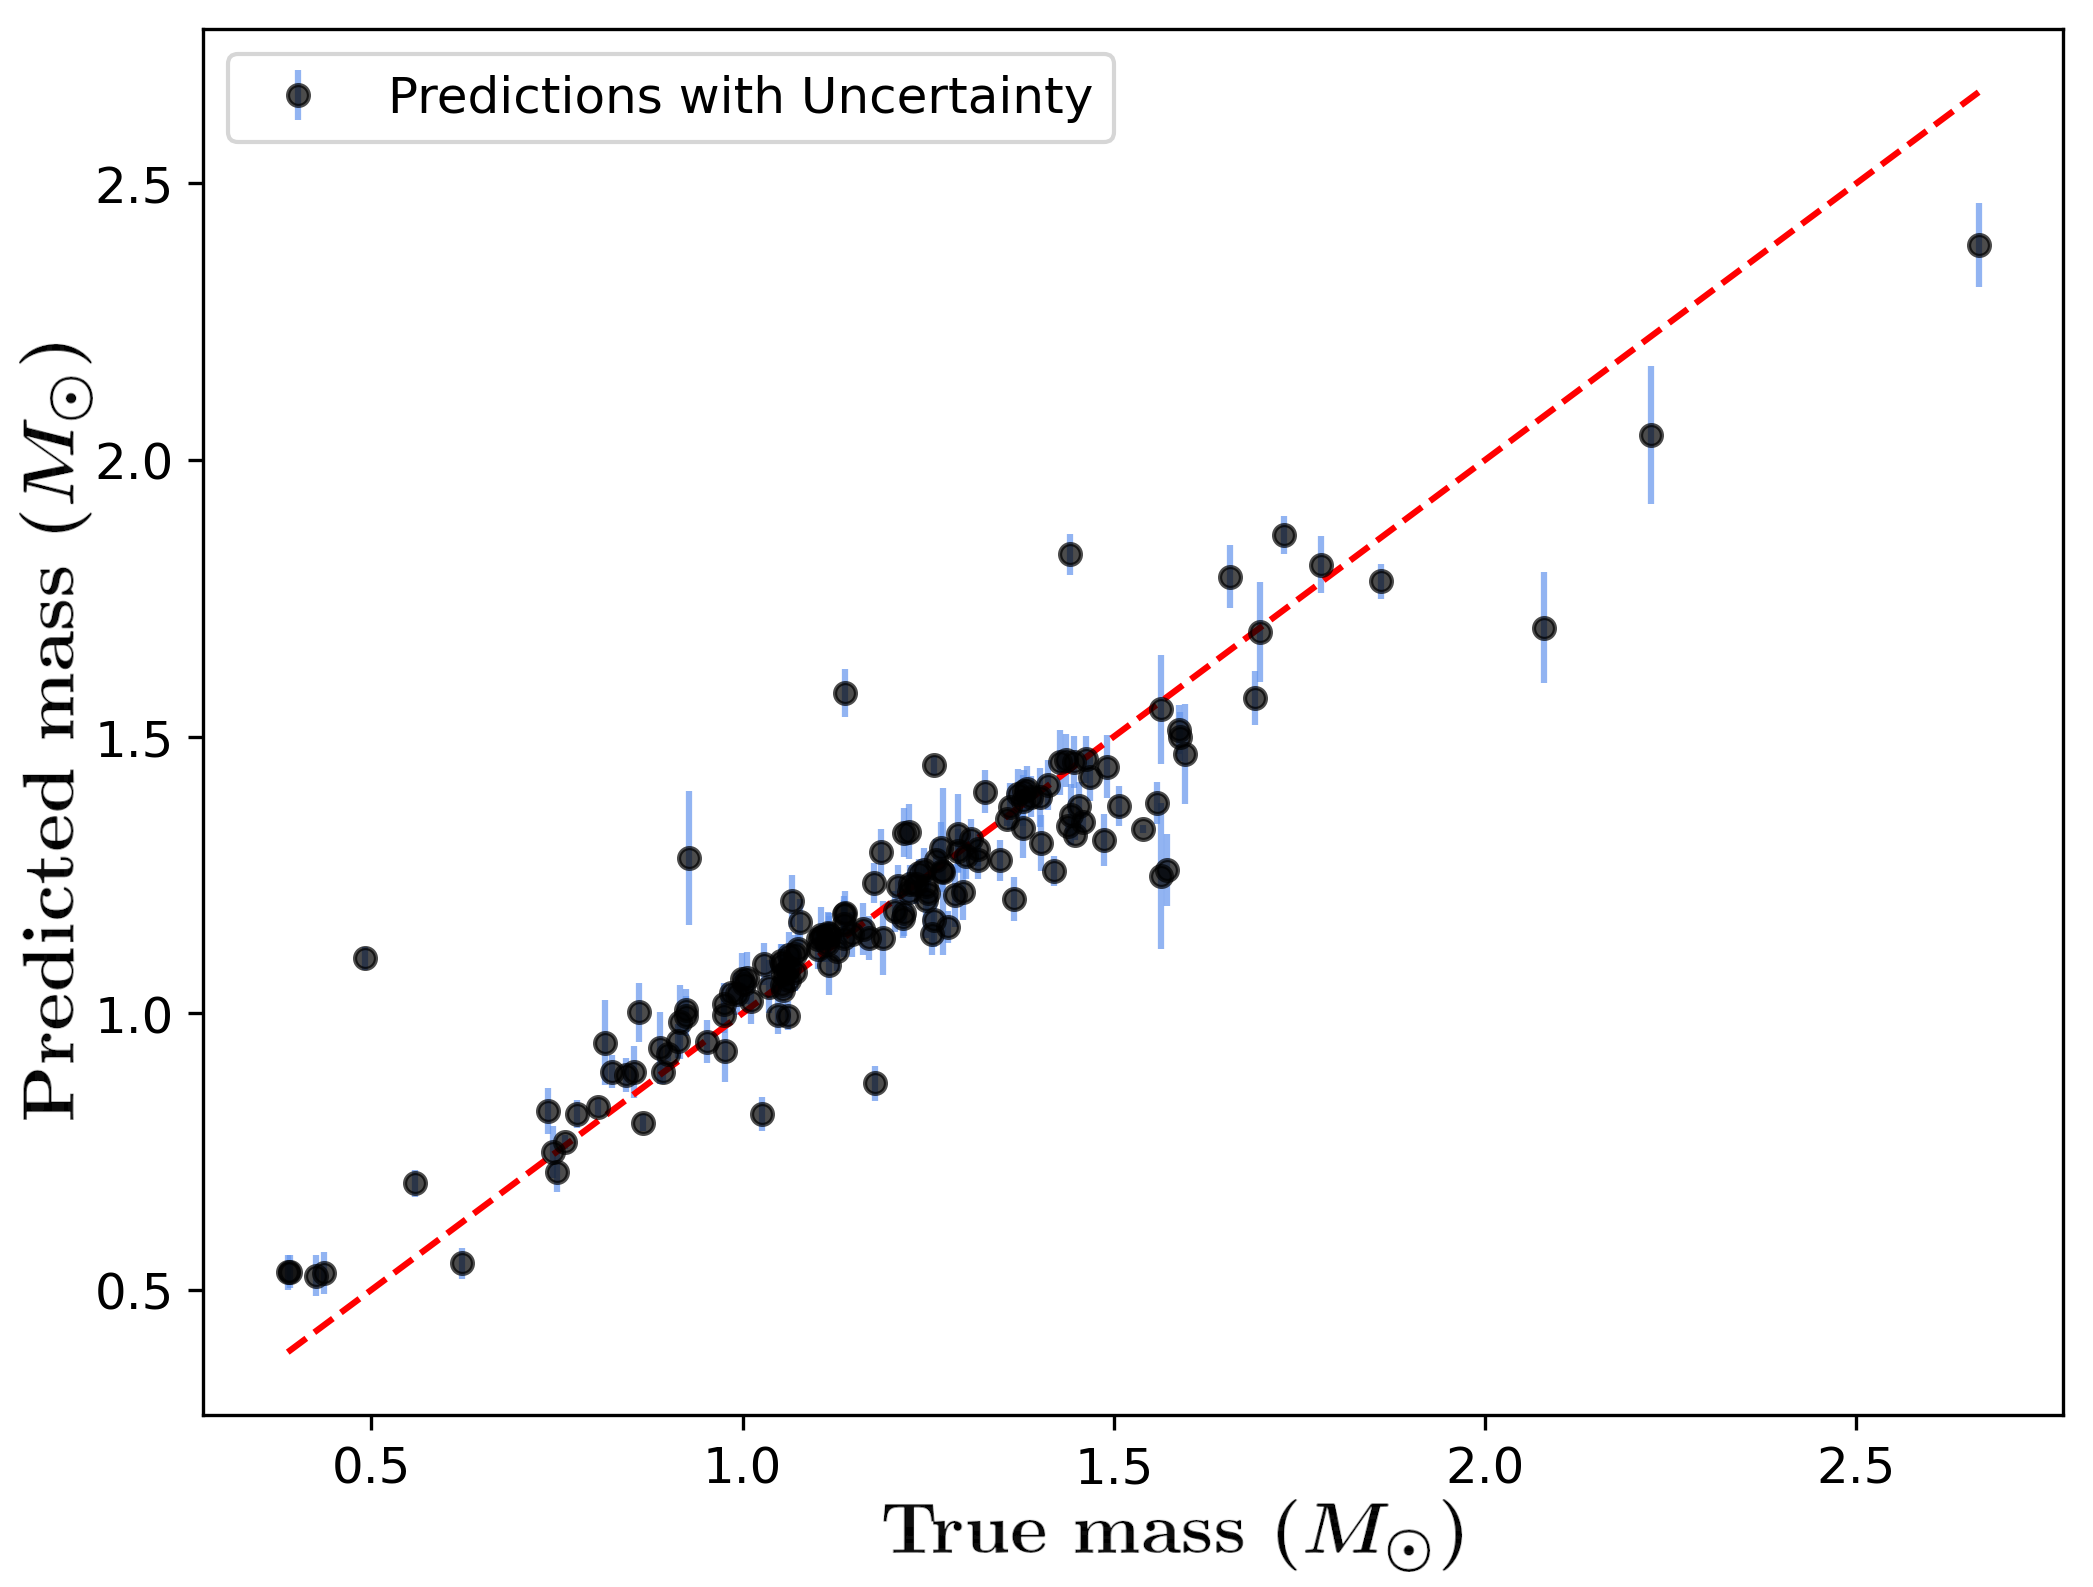
\includegraphics[width=\linewidth]{HBNN_mass_3param_L_1000_draws_4_chains_15_nodes_sig_015_seed_176_full_prediction_no_title_smaller_points_fontplus2.png}
\caption{HBNN prediction.}
\label{fig:hbnn_mass_predictions_B}
\end{subfigure}
\hfill
\begin{subfigure}[t]{0.24\textwidth}
\centering
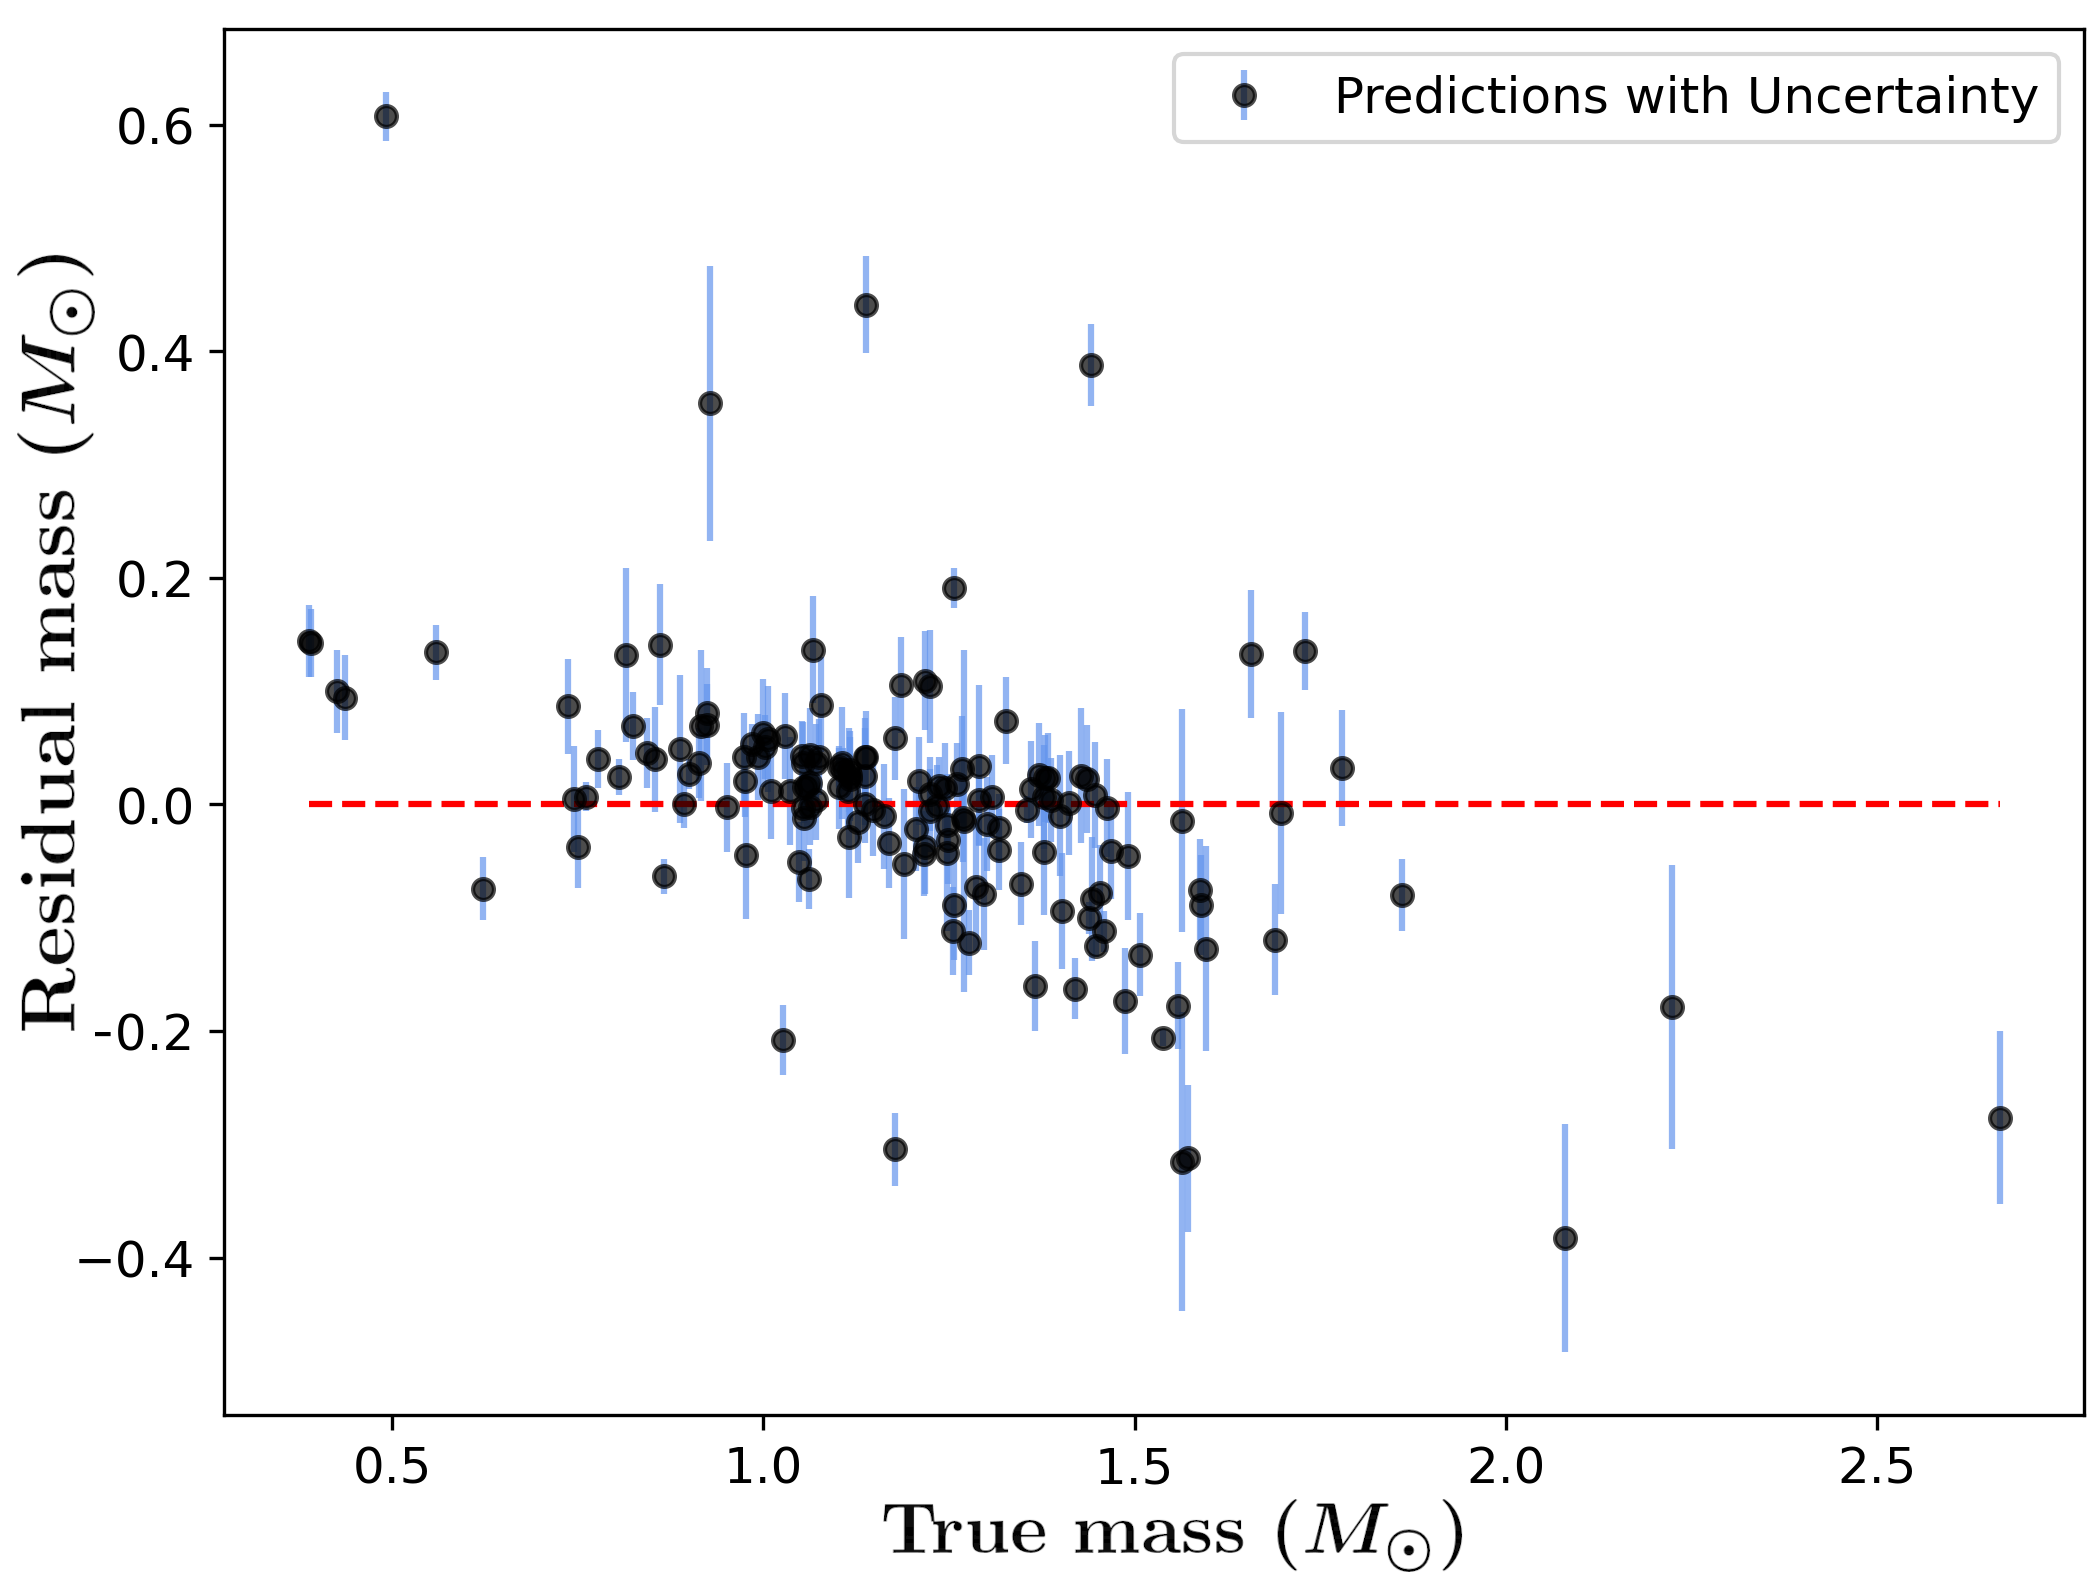
\includegraphics[width=\linewidth]{HBNN_mass_3param_L_1000_draws_4_chains_15_nodes_sig_015_seed_176_full_residual_no_title_smaller_points_fontplus2.png}
\caption{HBNN residuals.}
\label{fig:hbnn_mass_residuals_B}
\end{subfigure}
\hfill
\begin{subfigure}[t]{0.24\textwidth}
\centering
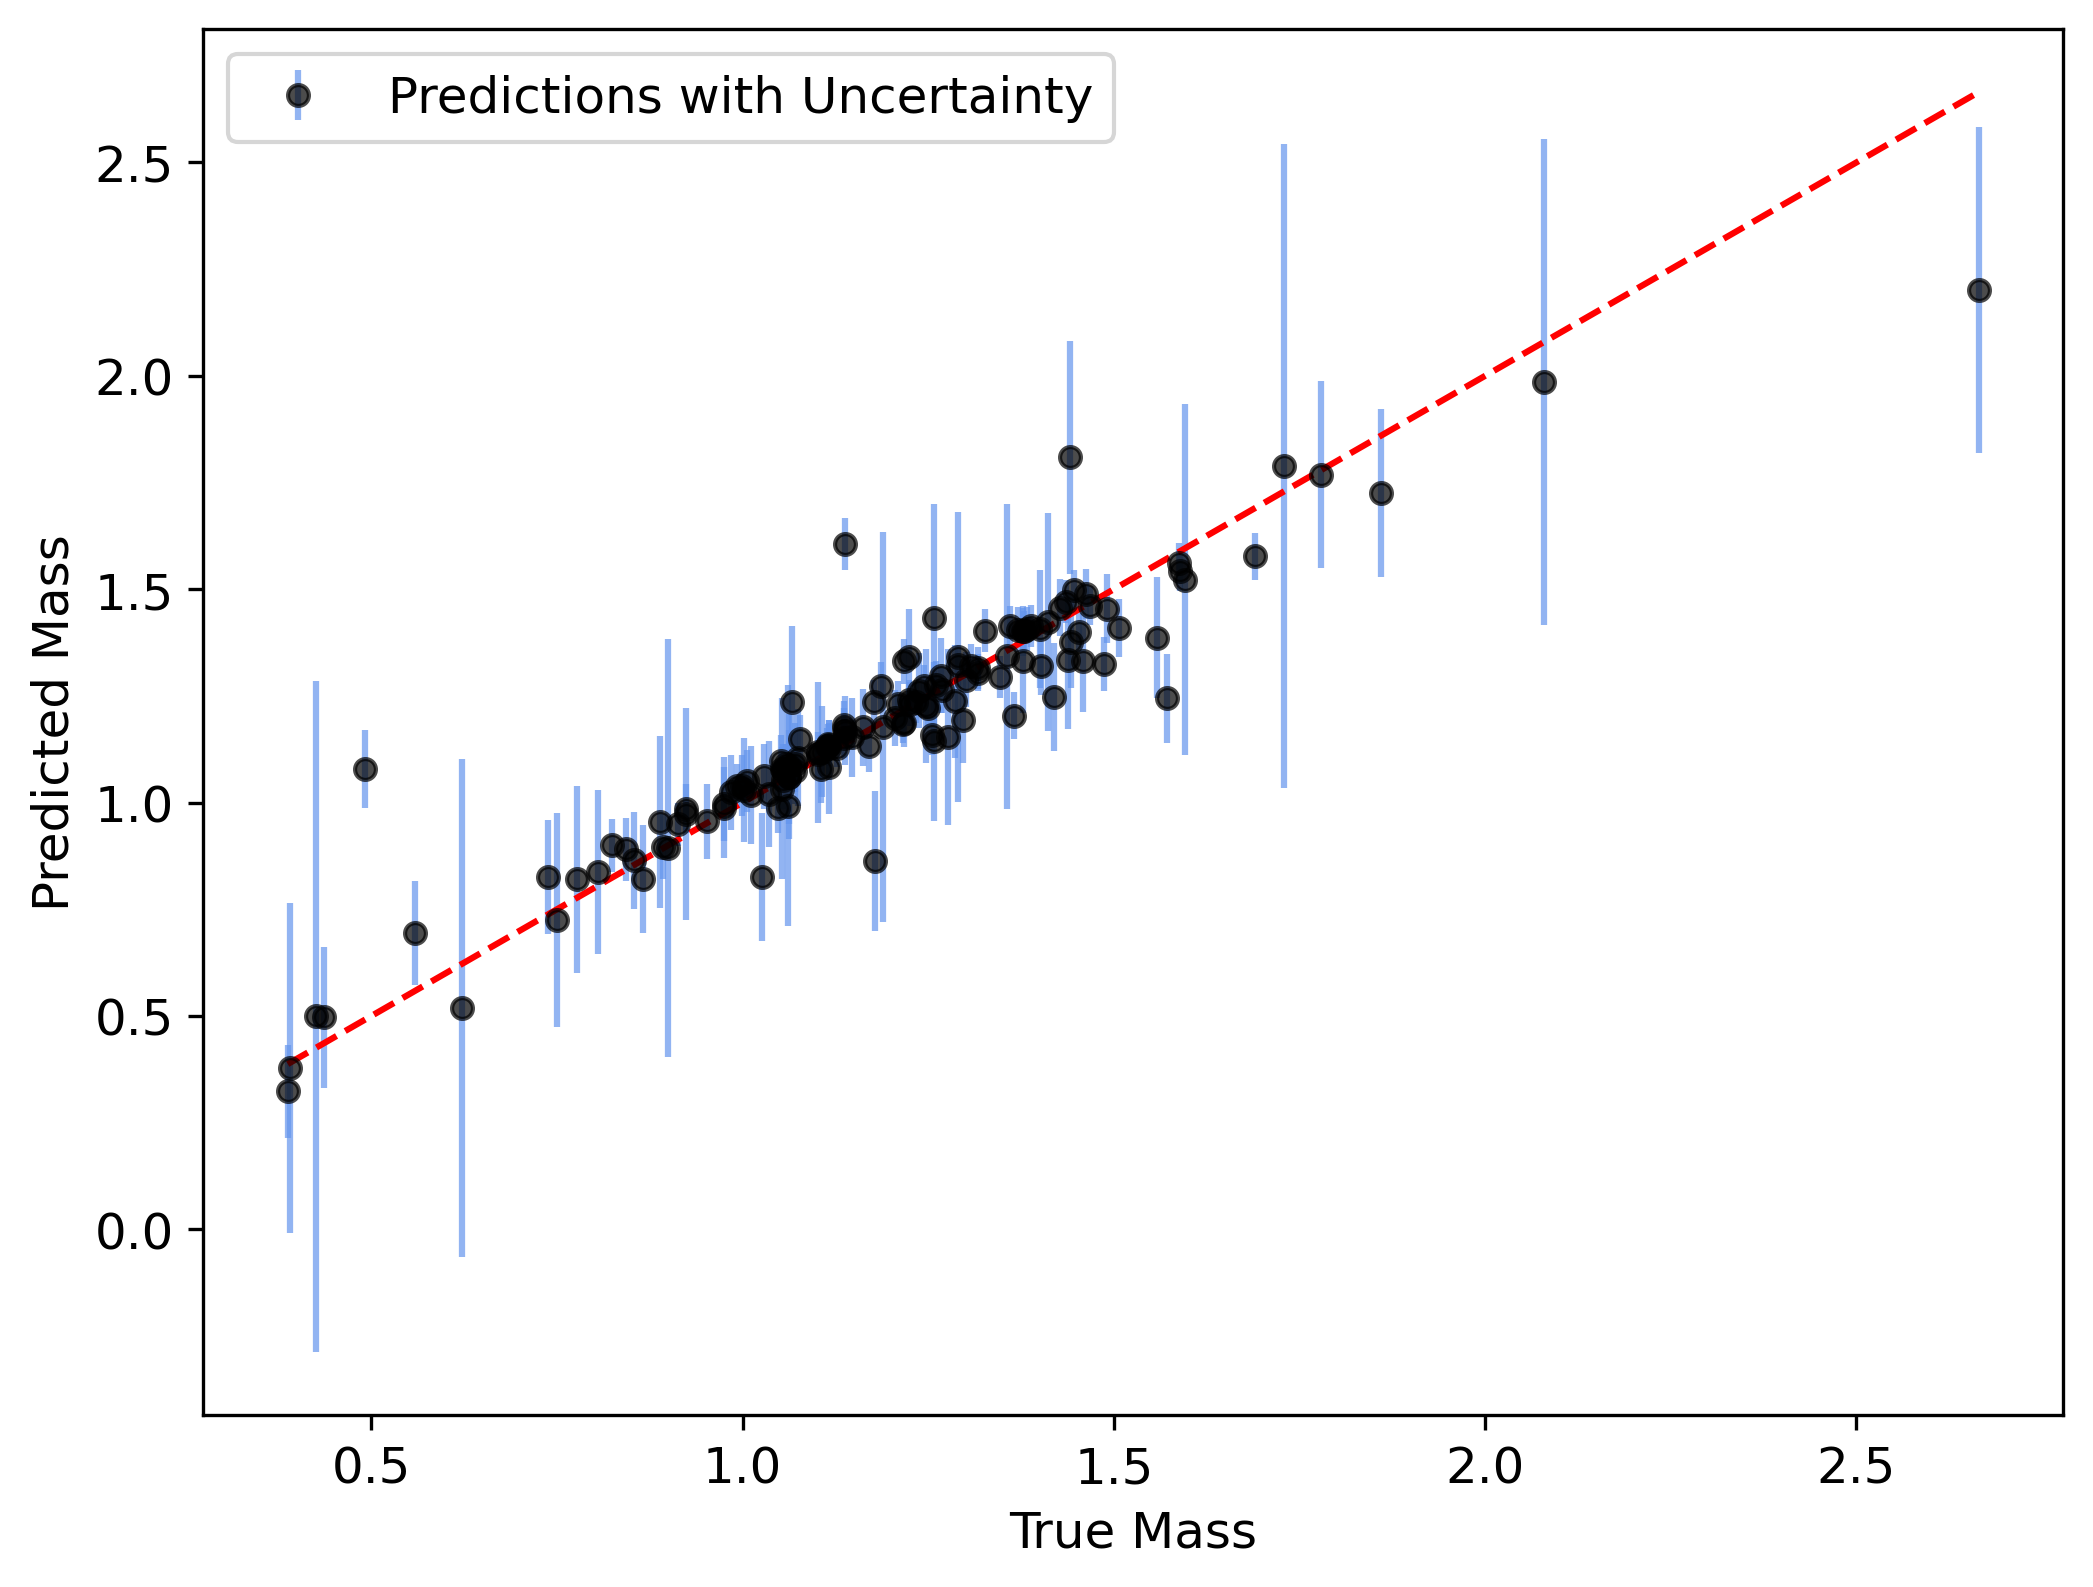
\includegraphics[width=\linewidth]{GP_mass_3param_L_1000_draws_4_chains_80_40_seed_176_filtered_90_prediction_no_title_smaller_points_fontplus2.png}
\caption{GP prediction.}
\label{fig:gp_mass_predictions_B}
\end{subfigure}
\hfill
\begin{subfigure}[t]{0.24\textwidth}
\centering
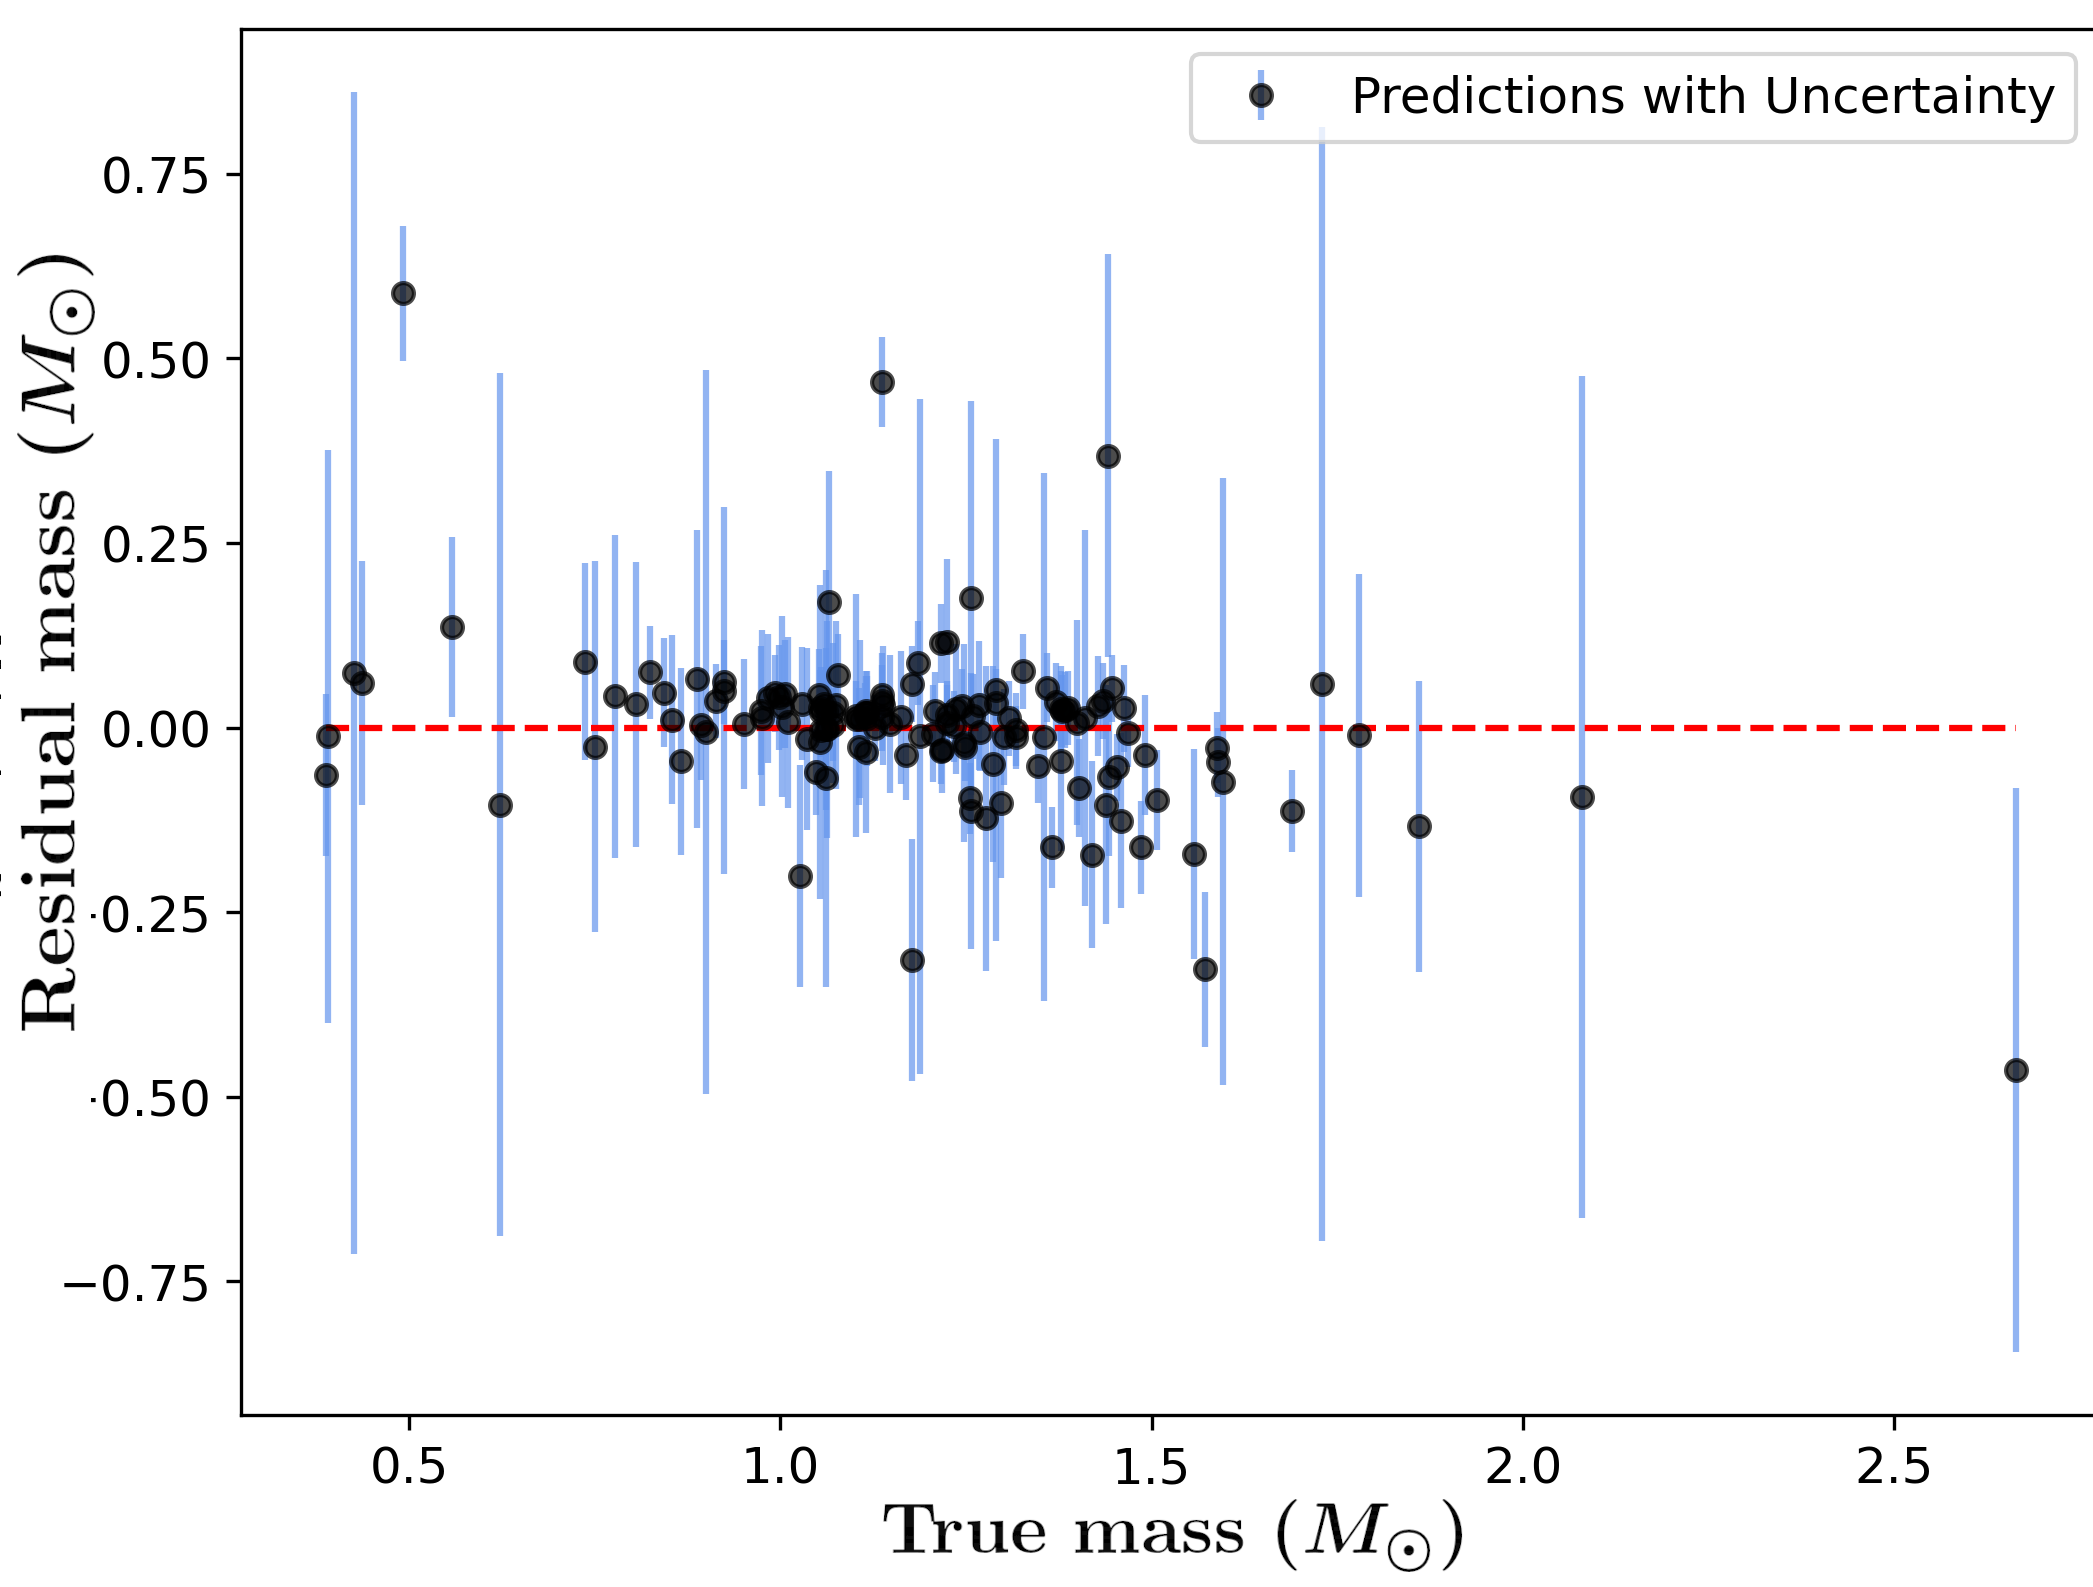
\includegraphics[width=\linewidth]{GP_mass_3param_L_1000_draws_4_chains_80_40_seed_176_filtered_90_residual_no_title_smaller_points_fontplus2.png}
\caption{GP residuals.}
\label{fig:gp_mass_residuals_B}
\end{subfigure}

\vspace{0.4cm}

% Bottom row: BART, BHS
\begin{subfigure}[t]{0.24\textwidth}
\centering
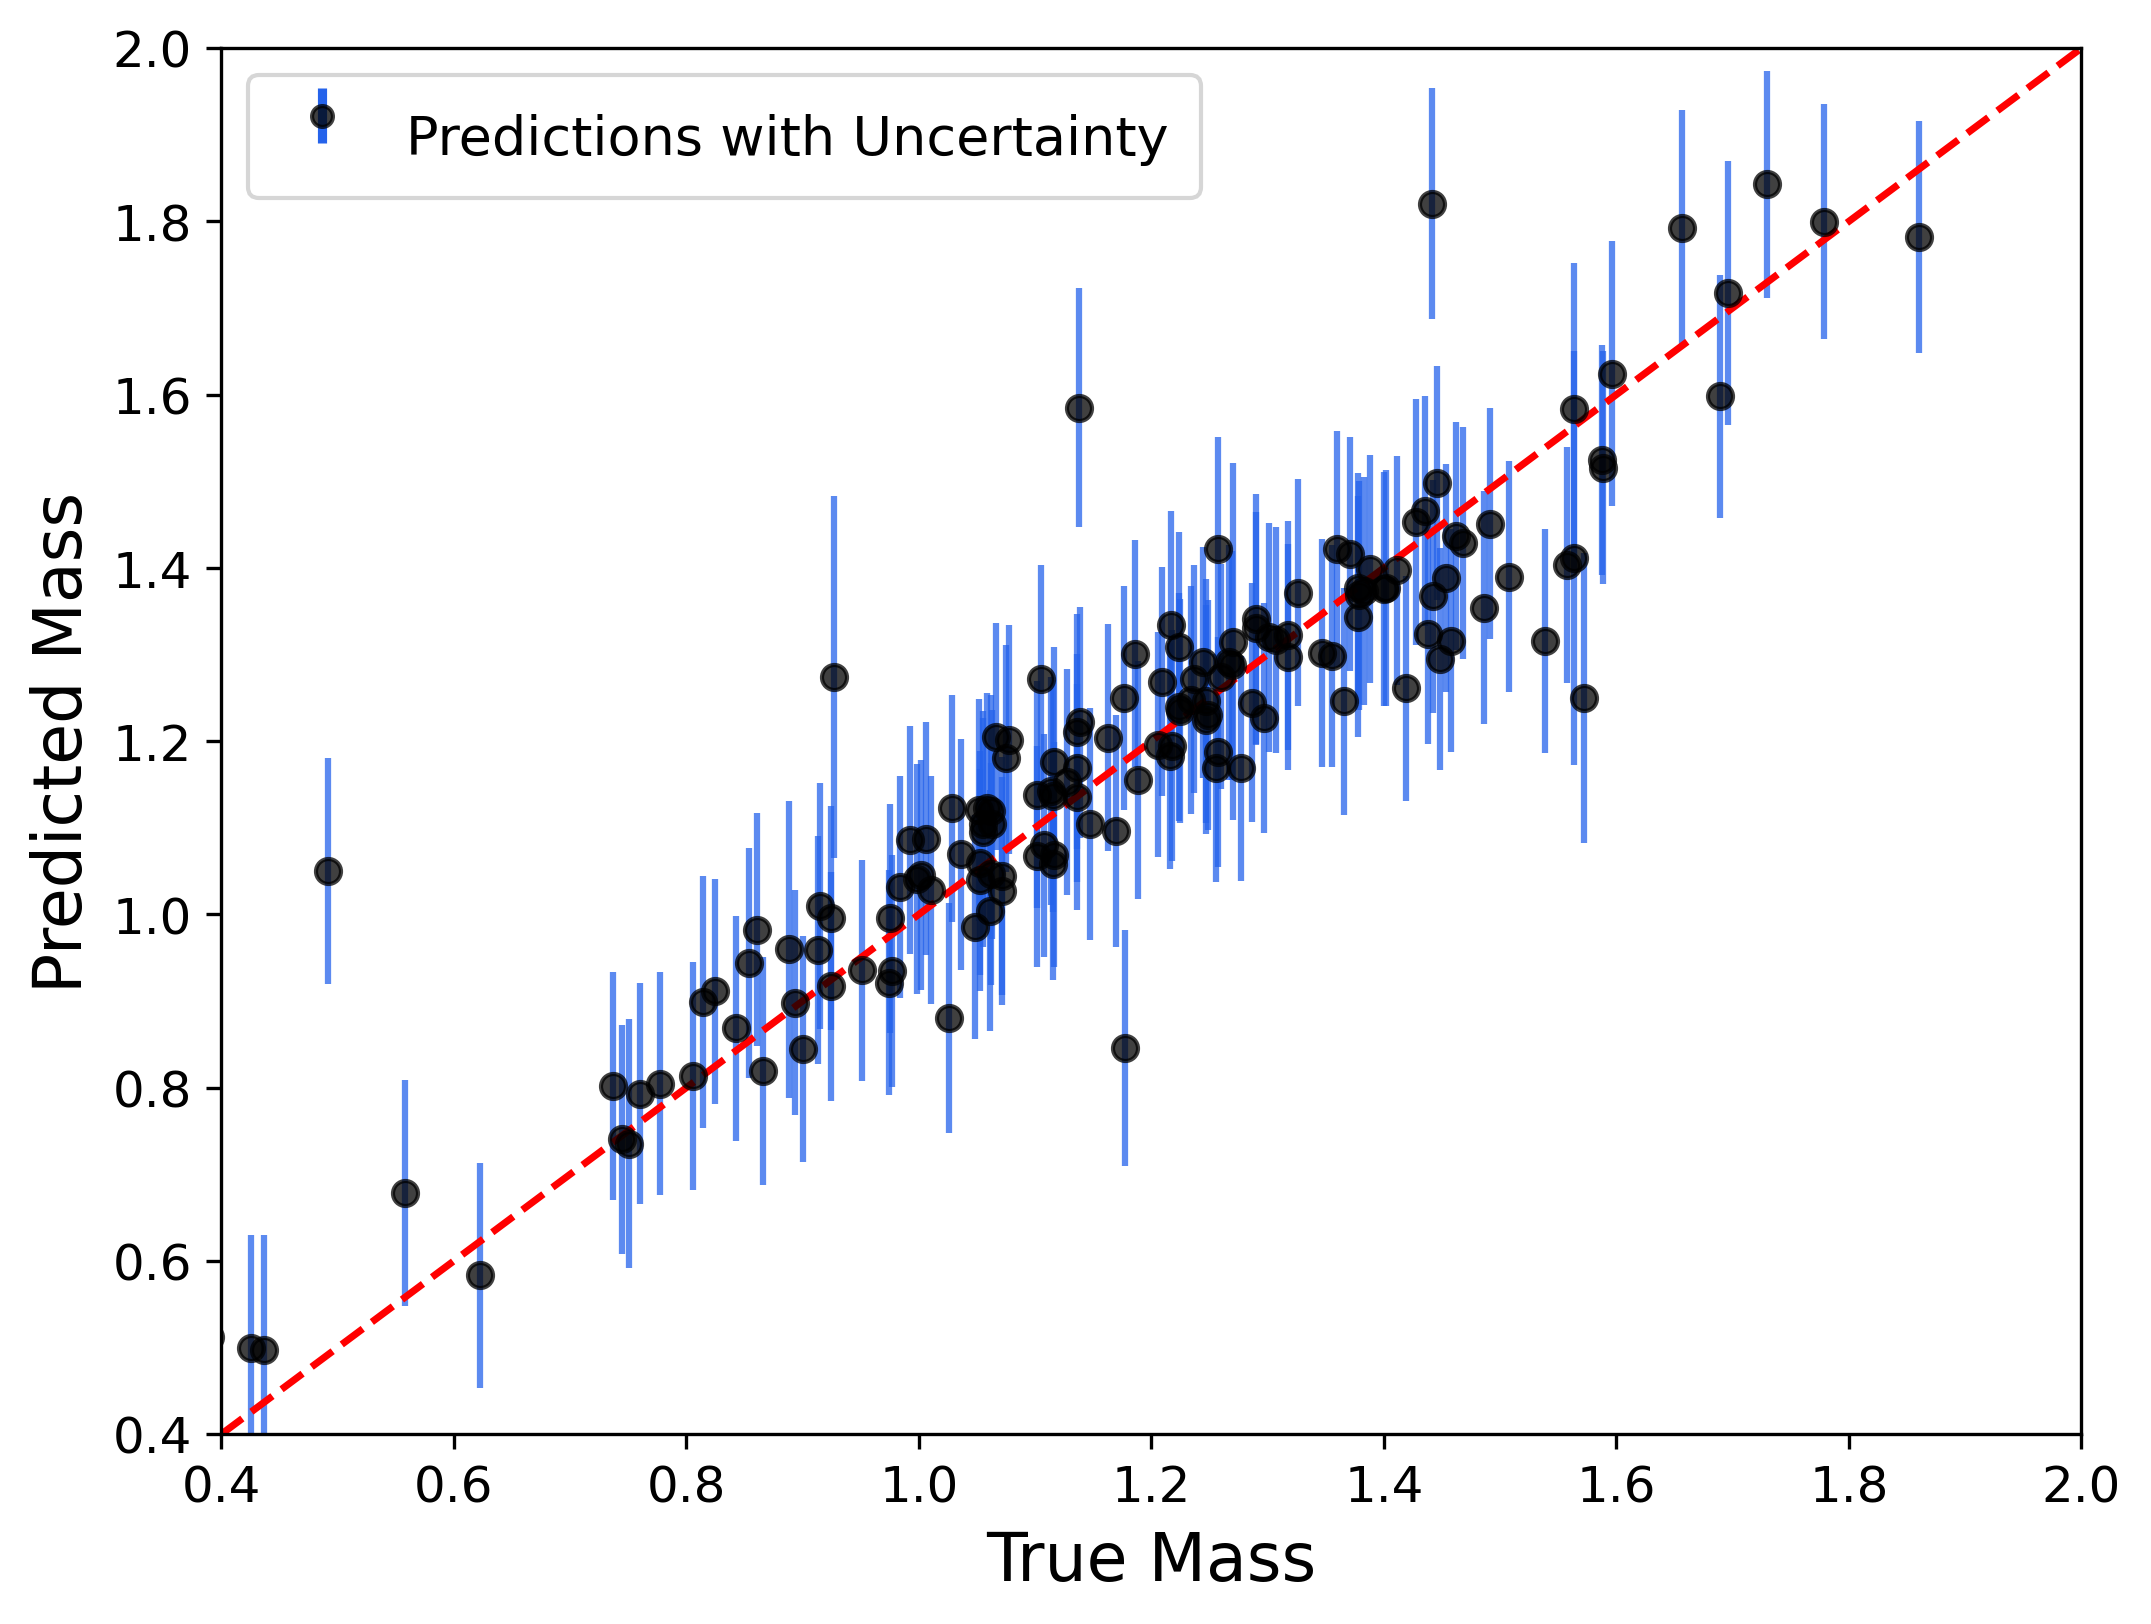
\includegraphics[width=\linewidth]{BART_mass_3param_L_prediction_seed_176_full_prediction_fontminus2_vertical_legend.png}
\caption{BART prediction.}
\label{fig:bart_mass_predictions_B}
\end{subfigure}
\hfill
\begin{subfigure}[t]{0.24\textwidth}
\centering
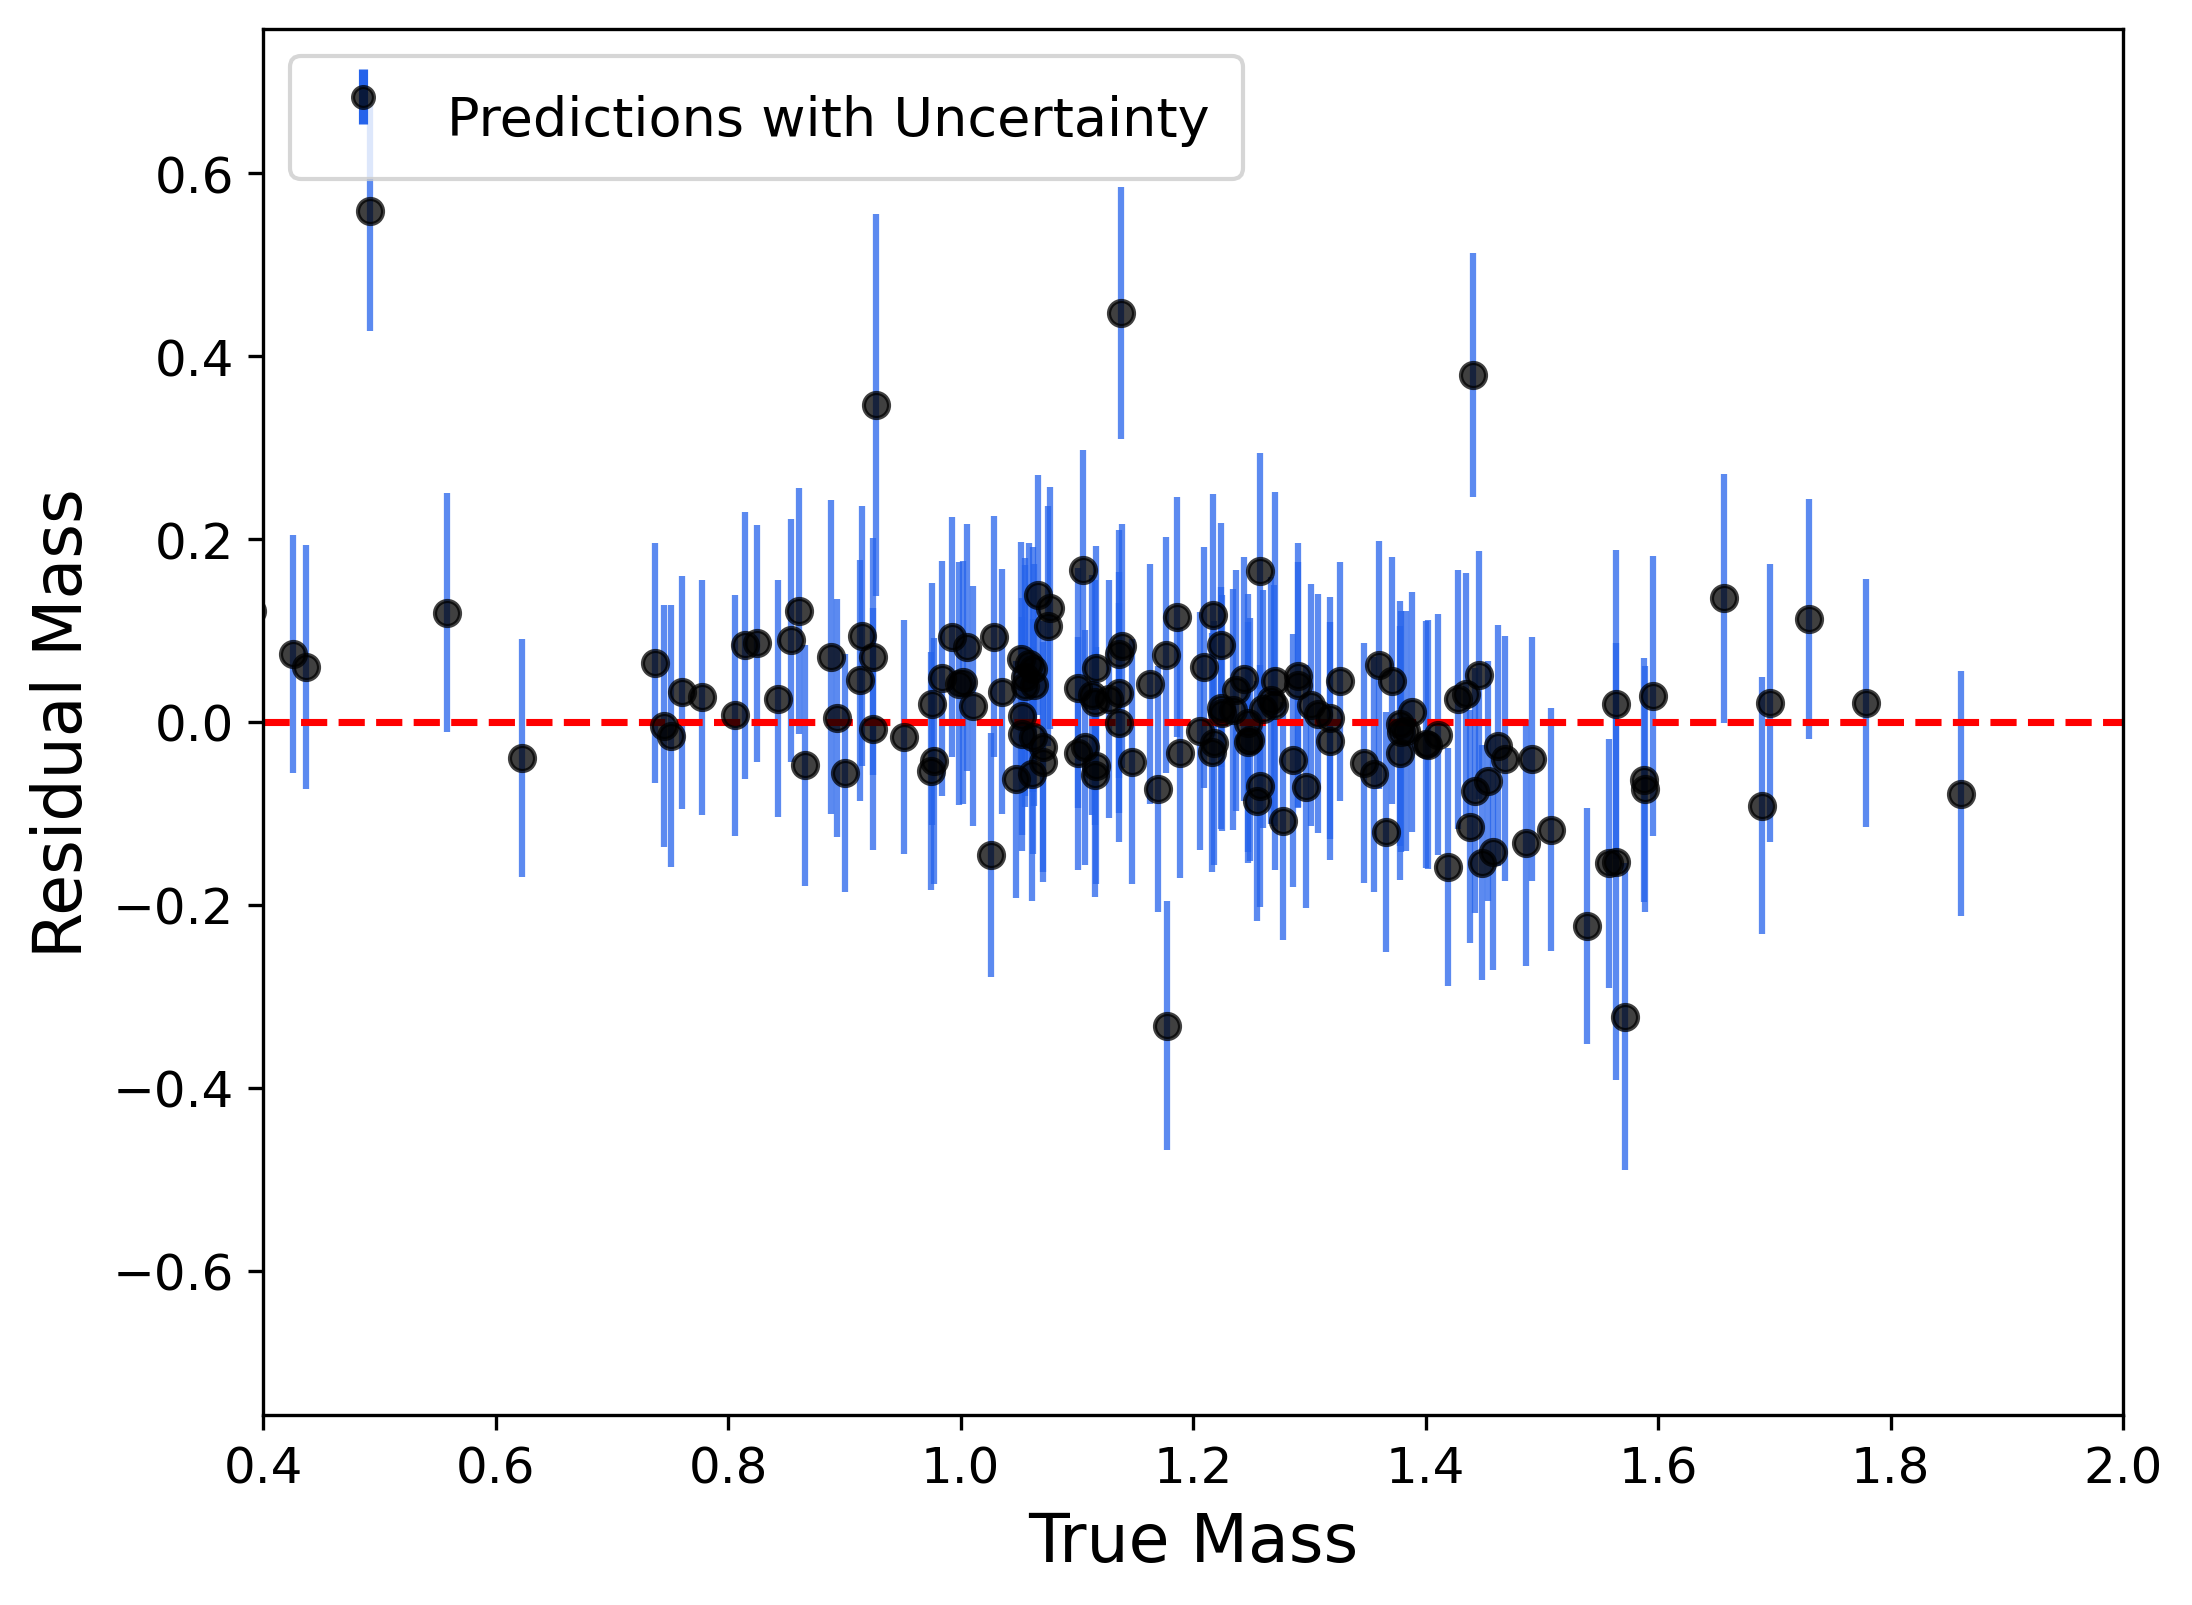
\includegraphics[width=\linewidth]{BART_mass_3param_L_prediction_seed_176_full_residual_fontminus2_vertical_legend.png}
\caption{BART residuals.}
\label{fig:bart_mass_residuals_B}
\end{subfigure}
\hfill
\begin{subfigure}[t]{0.24\textwidth}
\centering
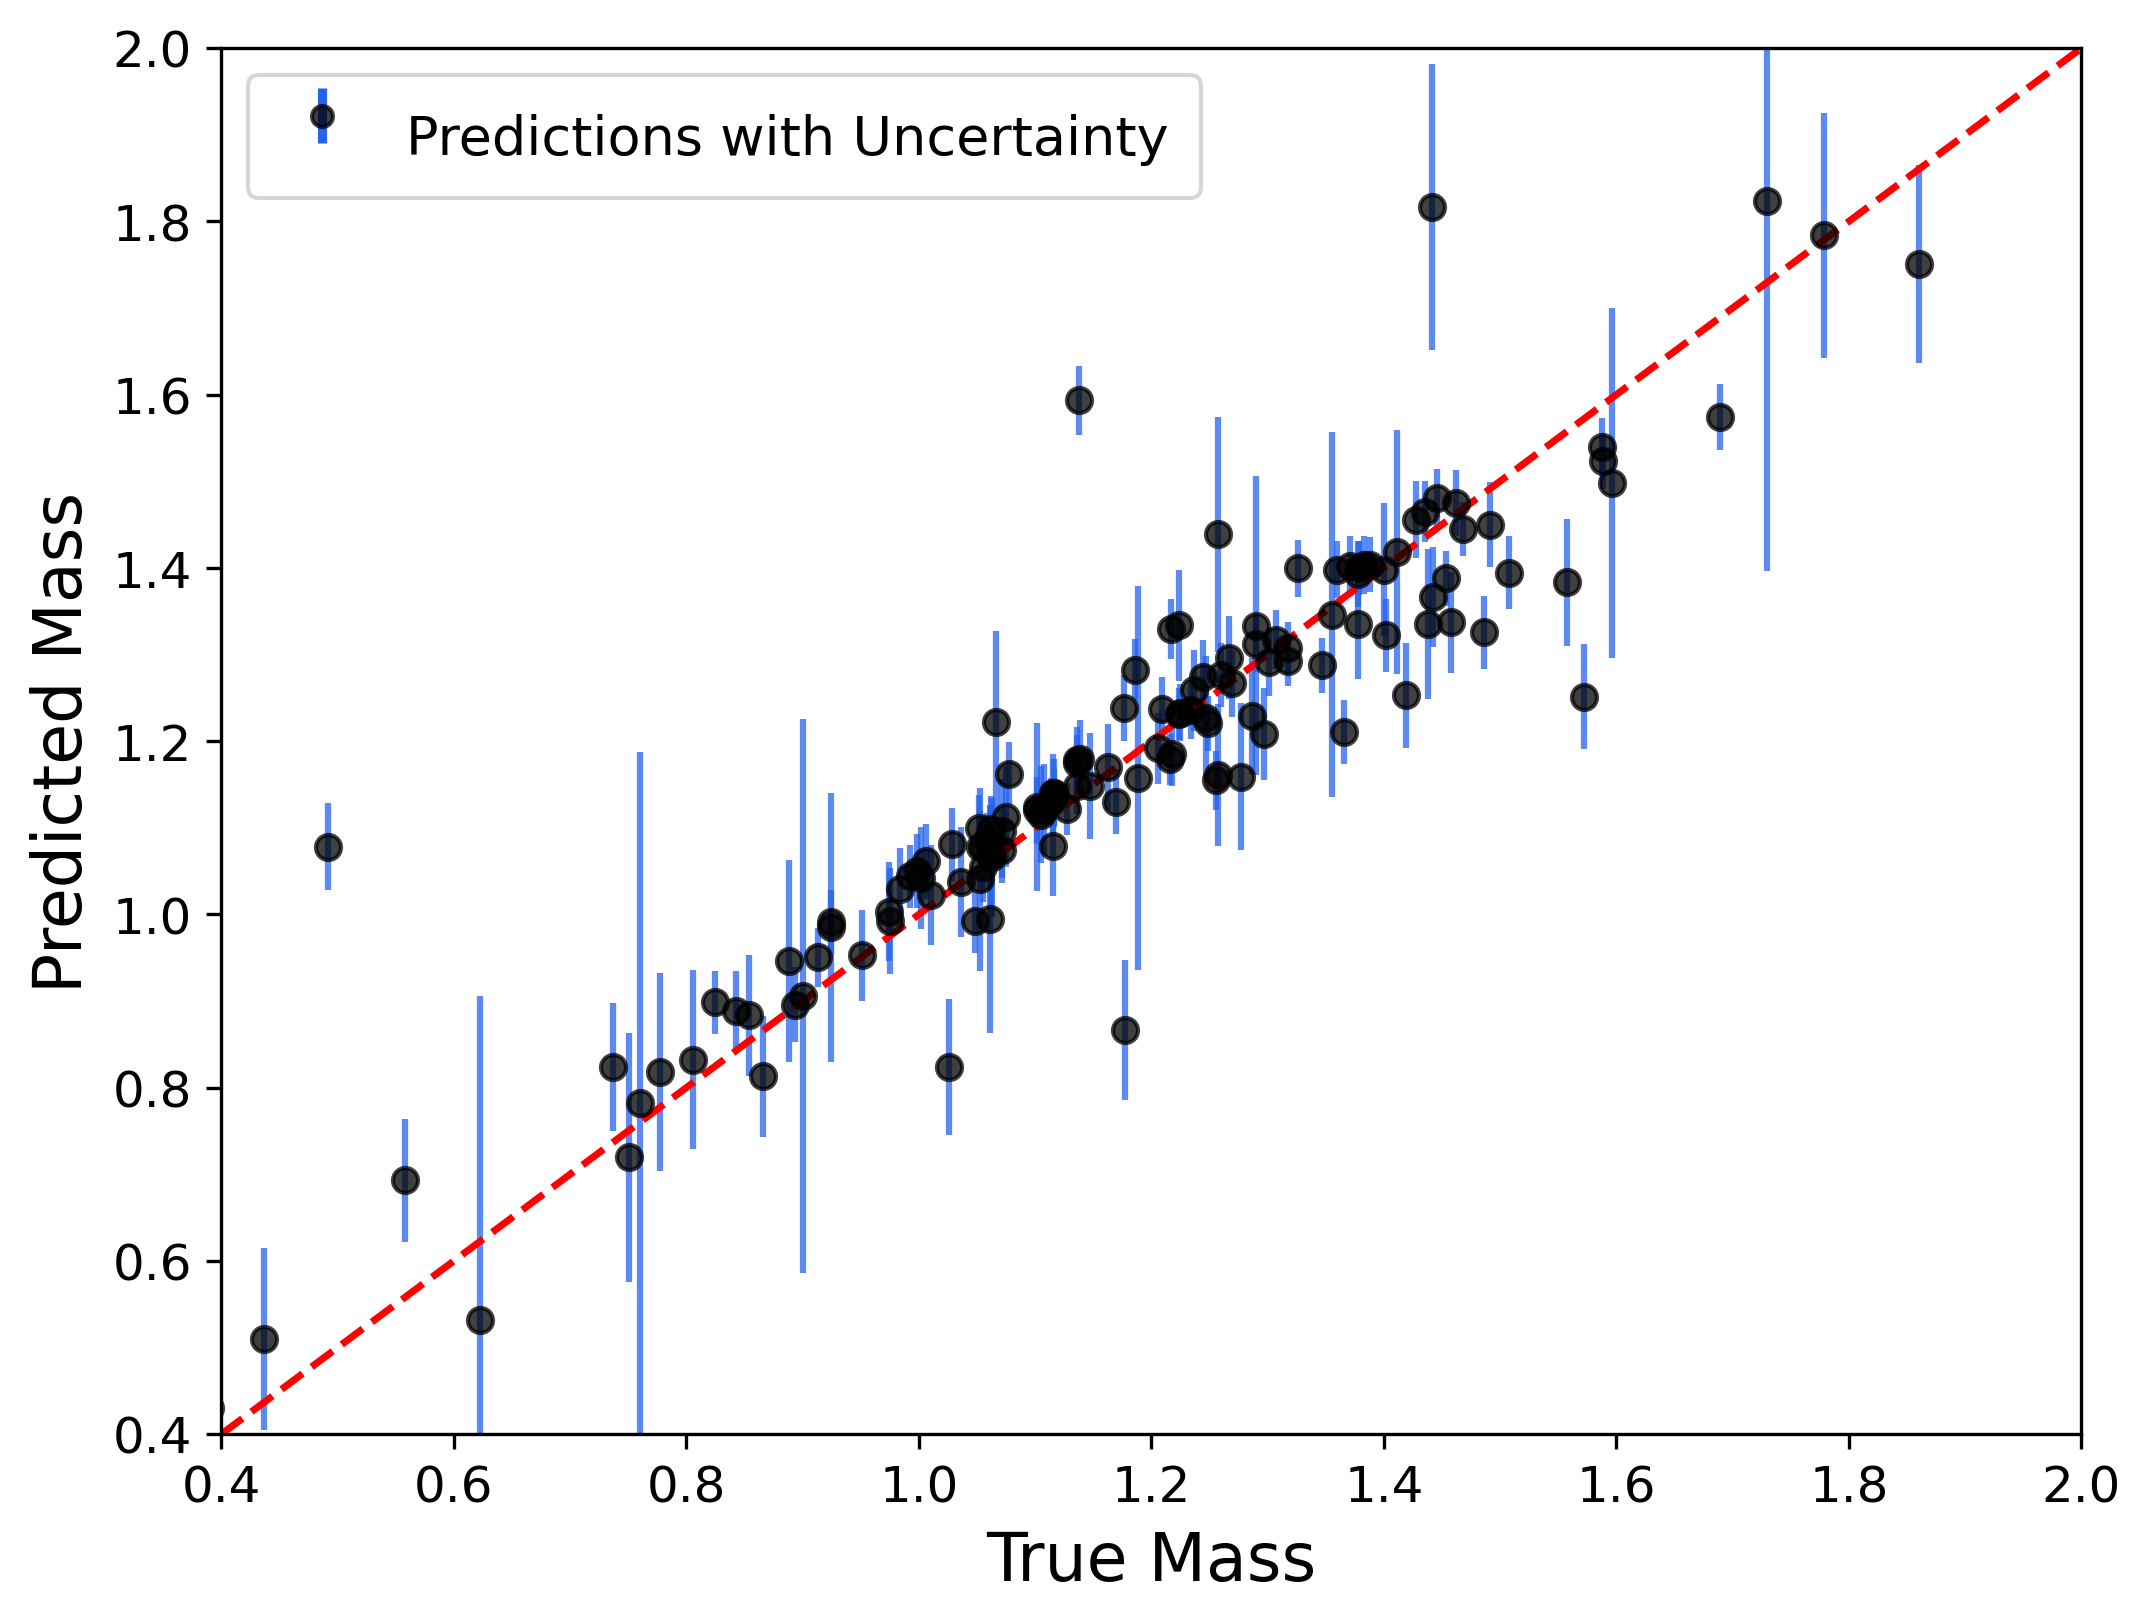
\includegraphics[width=\linewidth]{BHS_mass_3param_L_prediction_seed_176_filtered_90_prediction_fontminus2_vertical_legend.png}
\caption{BHS prediction.}
\label{fig:bhs_mass_predictions_B}
\end{subfigure}
\hfill
\begin{subfigure}[t]{0.24\textwidth}
\centering
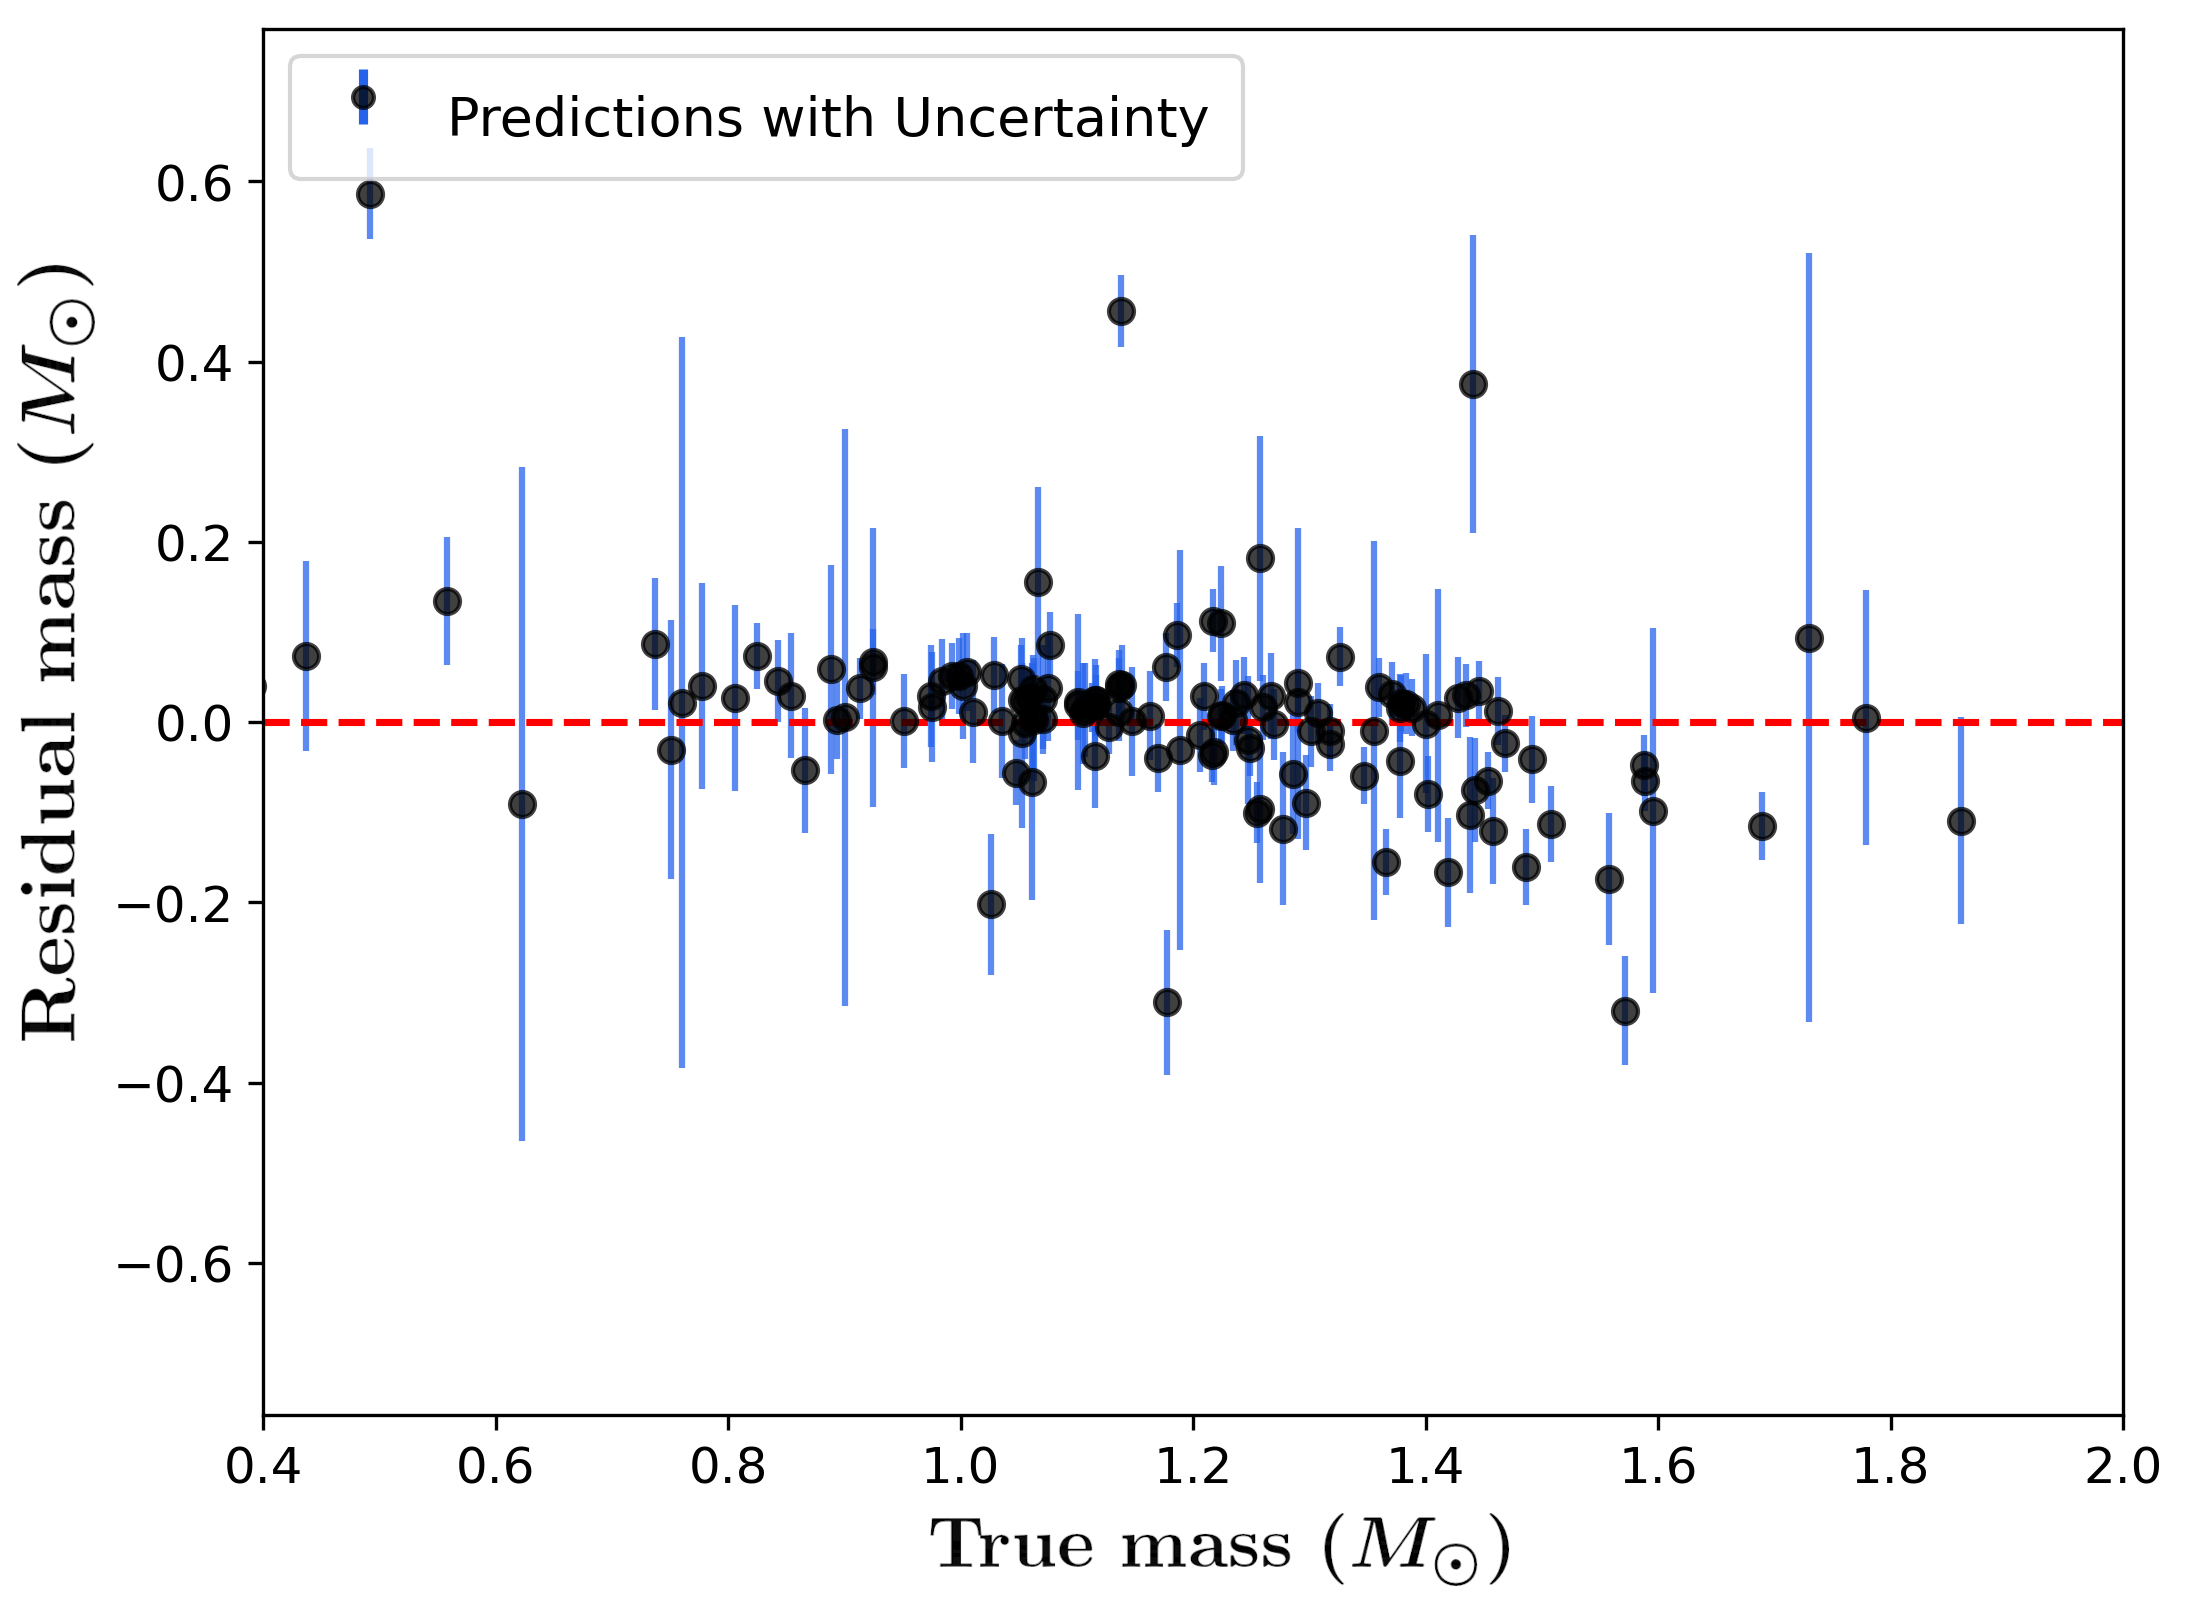
\includegraphics[width=\linewidth]{BHS_mass_3param_L_prediction_seed_176_filtered_90_residual_fontminus2_clear_vertical_legend.png}
\caption{BHS residuals.}
\label{fig:bhs_mass_residuals_B}
\end{subfigure}

\caption{Holdout-test performance of the HBNN, GP, BART and BHS mass models trained with $T_{\mathrm{eff}}$, $L$ and $[\mathrm{Fe}/\mathrm{H}]$. For each model, the prediction panel shows $M_{\mathrm{pred}}$ as a function of $M_{\mathrm{true}}$, while the residual panel shows $M_{\mathrm{pred}}-M_{\mathrm{true}}$ as a function of $M_{\mathrm{true}}$. Vertical error bars represent the predictive uncertainty returned by each model. The GP and BHS panels are restricted to the stars below the 95th percentile of predicted mass uncertainty in order to keep the main population visually readable. The full calibration sample contains $n=767$ stars, with $20\%$ reserved for the holdout test.}
\label{fig:mass_holdout_all_models_B}

\end{figure}

BHS combines the behaviours of the three level-0 models and remains the most stable compromise between residual accuracy and global bias. Since GP performs better away from $1\,M_\odot$ than BART and HBNN, the stacking approach is expected to assign it larger weight in those regions. In the central region, however, BHS can favour the other models when they provide more reliable predictions. Overall, the points remain well concentrated around the 1:1 relation, with no clear systematic trend. Although the BHS MRD is slightly worse than the GP value, this is expected because the stacking model does not simply reproduce the GP predictions, but balances them with the contributions of BART and HBNN. This behaviour is consistent with the evaluation metrics. The large individual predictive uncertainties of the stacking model suggest that it inherits part of the underconfidence already present in BART and GP, a behaviour also observed in the $\rho$-training case.


The mass predictions, including their uncertainties, are then compared with the stellar evolutionary-grid estimates based on PARSEC \citep{bressan2012} and with the linear-relation masses presented by \citet{moya2018}. The differences are analysed through fractional residuals, defined as $(M_1-M_2)/M_2$, where $M_1$ and $M_2$ correspond to the first and second methods indicated in each comparison label in Figure \ref{fig:frac_res_distrib_dataset_b}. The closest agreement is found between the BHS predictions and the grid-model masses: in this case, all residuals remain within approximately $\pm 10\%$. The stacking approach gives systematically higher masses than the grid models, but in a relatively homogeneous way, since both the mean and the median lie close to each other, near a fractional difference of $+2\%$.

When BHS is compared with the \citet{moya2018} linear relations, the behaviour changes, showing a more dispersed distribution with a tail of mass differences up to about $15\%$. The near-zero mean residual should not be interpreted as evidence that the stacking approach and the linear relations are consistently equivalent, but rather as the result of a broader residual distribution in which positive and negative deviations partly cancel. Table \ref{tab:residuals_dataset_b} confirms this interpretation: the mean residual is $-0.38\%$, while the mean absolute residual increases to $3.14\%$, larger than the BHS-grid comparison value of $2.86\%$. The two methods therefore provide different predictions for individual stars, even though their average signed offset is small.

\begin{figure}[H]
\centering
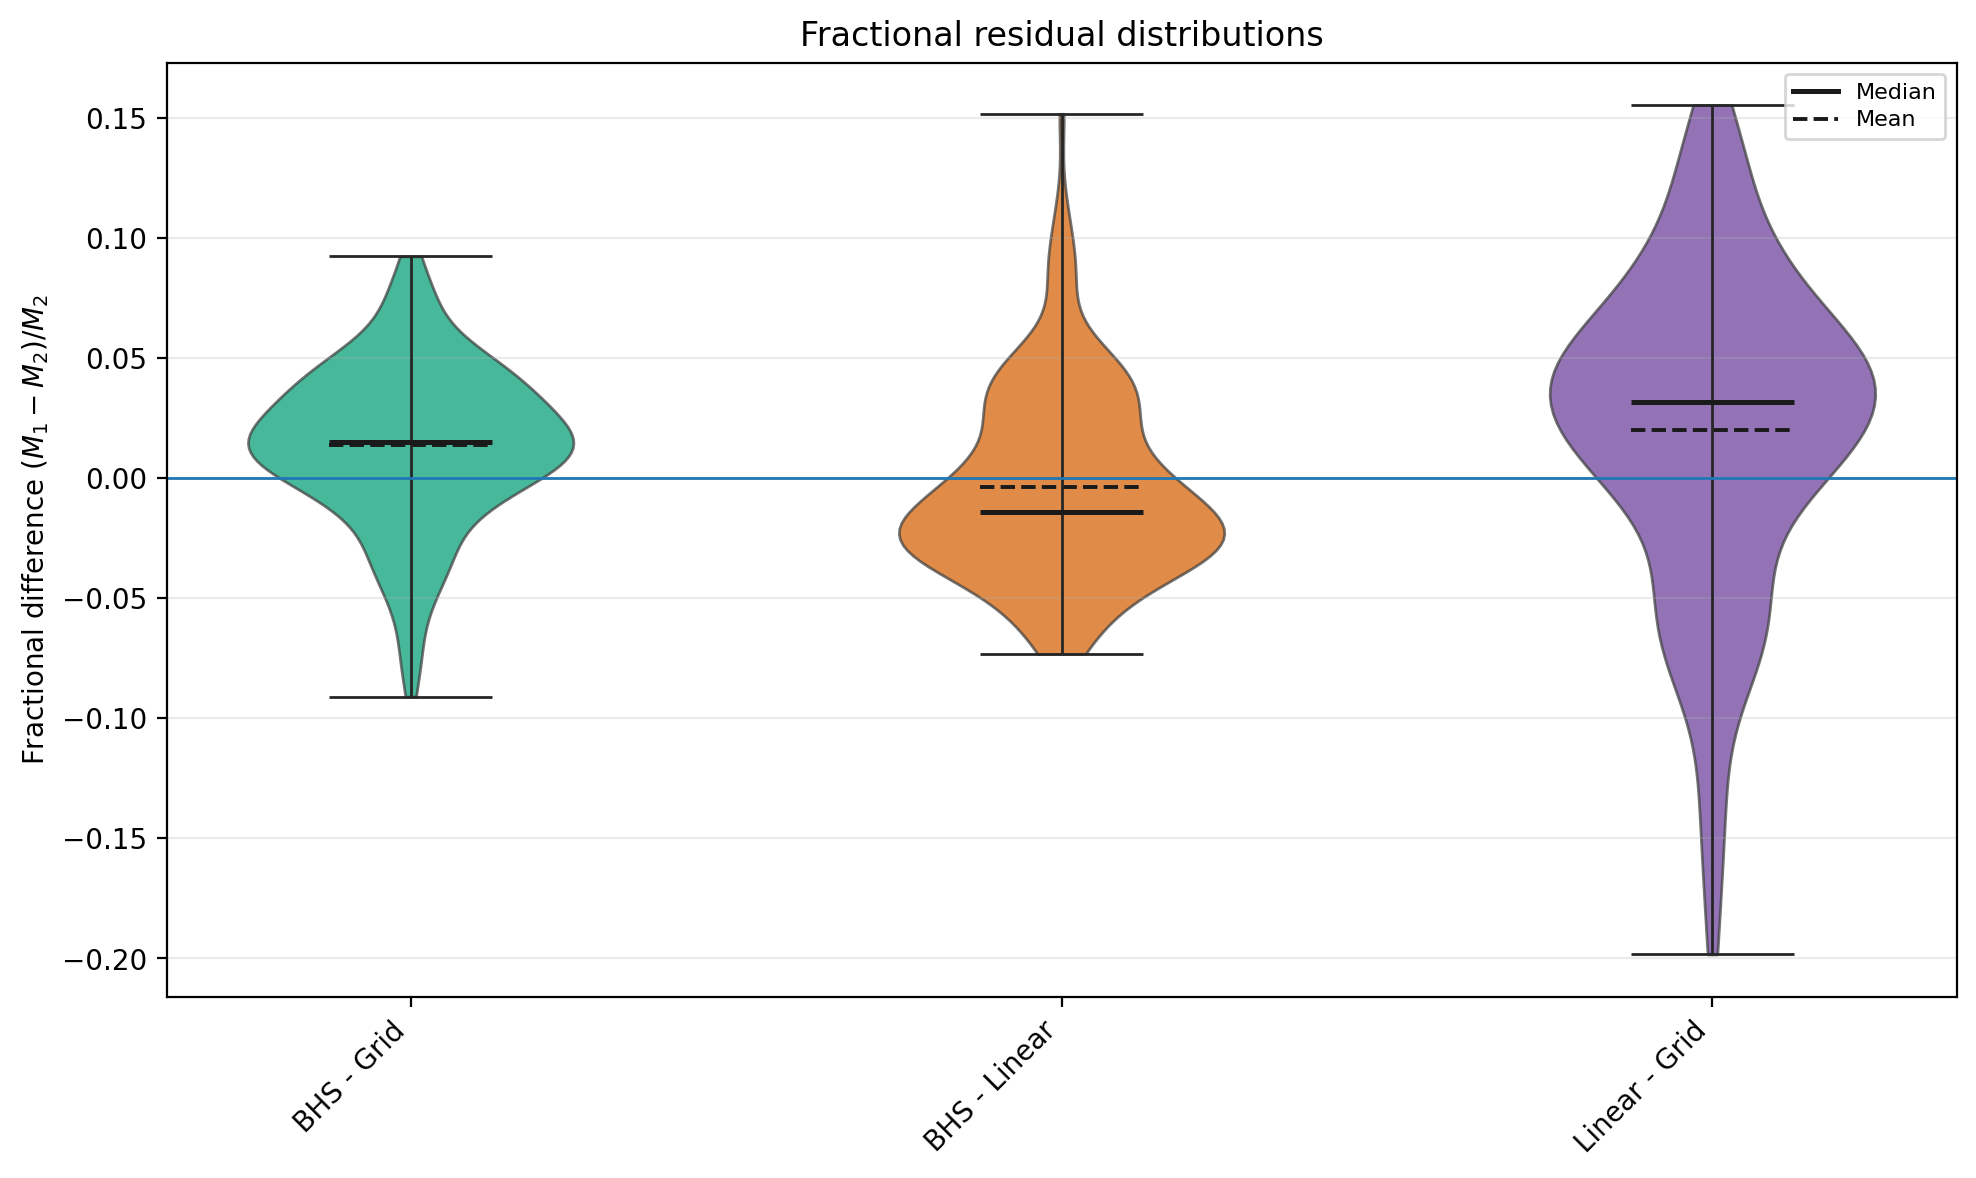
\includegraphics[width=0.8\linewidth]{mass_predictions_seed_819_without_bhs_2022_fractional_residual_distributions.png}
\caption{Distributions of fractional mass residuals for the comparison between the Bayesian Hierarchical Stacking predictions and the two reference mass estimates used for the ARIEL sample. The green distribution compares BHS with the stellar-model grid masses provided by the IA-Porto group, while the orange distribution compares BHS with the linear-relation masses from \citet{moya2018}. The purple distribution shows the direct comparison between the linear-relation and grid masses. The fractional residuals are defined as $(M_1-M_2)/M_2$, following the order of the two methods shown on the horizontal axis. The sample contains $n=184$ stars.}
\label{fig:frac_res_distrib_dataset_b}
\end{figure}

The two reference models do not produce equivalent predictions either. Figure \ref{fig:frac_res_distrib_dataset_b} and Table \ref{tab:residuals_dataset_b} show that the linear-relation and grid masses differ more strongly from each other than BHS differs from either of them, with a MARD above $5\%$ and a broad residual distribution that includes a tail of large negative residuals extending almost to $-20\%$. This tail is consistent with the one observed in the BHS-linear comparison, suggesting that the linear relations produce comparatively low masses for a small number of stars.

\begin{table}[H]
\centering
\caption{Mass-comparison metrics for the ARIEL sample using the same fractional-residual convention as in Figure \ref{fig:frac_res_distrib_dataset_b}.}
\begin{tabular}{lccc}
\hline\hline
Metric & BHS - Grid & BHS - Linear & Linear - Grid \\
\hline
MAE ($M_\odot$) & $0.031$ & $0.035$ & $0.061$ \\
MARD [\%] & $2.86$ & $3.14$ & $5.60$ \\
MRD [\%] & $1.39$ & $-0.38$ & $2.01$ \\
\hline
\end{tabular}
\label{tab:residuals_dataset_b}
\end{table}

\subsection{Oblateness and mass predictions of eclipsing binaries} \label{sec:dataset_C}
As explained in Section \ref{subsec:dataset_a}, one of the aims of this work is to predict the masses of FGK-type components in eclipsing-binary systems, so that information can then be inferred for their difficult-to-study M-type companions. Eclipsing binaries therefore provide one of the most useful routes for obtaining information about these objects, but it must be assessed whether the information inferred from stars in eclipsing-binary systems can be extrapolated to isolated stars of similar type.

Eclipsing-binary components are not completely independent objects. Their mutual gravitational interaction can modify their morphology through tidal forces, preventing them from remaining perfectly spherical. This distortion can be quantified through the oblateness parameter $o$, given by Equation (43) of \citet{chandrasekhar1933double}, which classifies stars from perfectly spherical ($o=0$) to highly oblate ($o \sim 1$):

\begin{equation}
o = 0.6446 \cdot \left(1 + 4\frac{m}{m_\star}\right) \cdot \left(\frac{R_\star}{a}\right)^3,
\label{eq:oblateness}
\end{equation}
where $R_\star$ and $m_\star$ are the radius and mass of the star whose oblateness is being computed, $m$ is the mass of its companion, and $a$ is the orbital semi-major axis.

To test whether this tidal distortion affects the mass predictions, the models are trained on asteroseismic stars, which are treated here as the single-star reference sample. Predictions are then obtained for the eclipsing-binary components available in the catalogue. The predicted masses are compared with the reference masses of the eclipsing-binary stars, and the resulting residuals are analysed as a function of oblateness. This follows the general approach of \citet{maxted2023benchmark}, where eclipsing binaries are used to evaluate how well single-star relations can be transferred to binary systems.

\subsubsection*{Results: holdout test}
The models were trained using the asteroseismic stars from the dataset in Table \ref{MS_catalog_database_D}. Since the goal in this section is to obtain accurate mass predictions before analysing the residual dependence on oblateness, four input features were used, following the recommendation of \citet{moya2022}: $T_{\mathrm{eff}}$, $\log g$, $L$ and $[\mathrm{Fe}/\mathrm{H}]$. This subset contains 420 stars, of which 84 were retained as the holdout set. There are therefore two competing effects on the predictive performance of the models. On the one hand, the models now use four input features instead of three, which should improve the precision of the predictions. On the other hand, the available sample is reduced from the original 767 stars to 420 stars. 

\begin{table}[H]
    \centering
    \caption{Comparison of the residual metrics obtained by the mass-prediction models on the holdout set. The models were trained with $T_{\mathrm{eff}}$, $\log g$, $L$ and $[\mathrm{Fe}/\mathrm{H}]$ as input features, and stellar mass as the target.}
    \label{tab:dataset_D_model_mard_mrd}
    \begin{tabular}{lcccc}
        \hline\hline
        Metric & BART & GP & HBNN & BHS \\
        \hline
        MAE ($M_\odot$) & $0.052$ & $0.042$ & $0.045$ & $0.043$ \\
        MARD [\%] & $4.50$ & $3.84$ & $3.98$ & $3.85$ \\
        MRD [\%]  & $-0.99$ & $-0.69$ & $-0.61$ & $-0.65$ \\
        \hline
    \end{tabular}
\end{table}

The predictions and residuals behave similarly to those discussed in Figure \ref{fig:mass_holdout_all_models}. The characteristic GP behaviour, with a small number of objects showing extremely large predictive uncertainties, is still present, reinforcing the interpretation that the effect is mainly related to the model and its uncertainty treatment, rather than to a fixed set of problematic stars. For HBNN and BART, the systematic behaviour away from $M=1\,M_\odot$ is observed and appears slightly amplified, as seen in Table \ref{tab:dataset_D_model_mard_mrd}. This indicates that, when the models are trained only with asteroseismic stars, the predictions develop a stronger signed bias. However, with $\log g$ included, the resulting metrics have lower values than those of Section \ref{subsec:dataset_b} (Table \ref{tab:dataset_b_mard_mrd}), consistently with the results of \citet{moya2022}.

The stronger signed bias is expected, since the training sample is now less heterogeneous. As shown in Figure \ref{fig:HRdiagram}, the asteroseismic stars are concentrated in a relatively narrow mass range, approximately between $0.8\,M_\odot$ and $1.5\,M_\odot$. This makes the predictions more robust within this specific region of the mass spectrum. Since the holdout test is evaluated against asteroseismic stars from the same population, which mostly occupy the same region of the HR diagram, MARD consequently decreases. However, the predictive performance is expected to be less reliable for stars outside this range, where systematic trends are reflected in the larger absolute MRD values.

Regarding the stacking model, BHS yields the best or nearly best predictions across the evaluated metrics. Although HBNN has a slightly lower MRD, this may reflect the cancellation of systematic overpredictions and underpredictions, as discussed in previous sections. BHS instead provides a more balanced compromise: its MARD is almost identical to that of GP, and its absolute MRD remains well below $1\%$.

\subsubsection*{Results: oblateness}
The effect of binary interaction was studied by predicting the masses of the stars in the original dataset that belong to eclipsing-binary systems. From this group, only systems with an available orbital semi-major axis $a$ could be used, since this parameter is required to compute the oblateness. As explained in Section \ref{sec:cleaning}, this leaves 295 stars with available oblateness estimates before applying the final selection cuts. Once $o$ was computed, the models trained on the asteroseismic stars were applied to these eclipsing-binary components, and the resulting mass residuals were analysed as a function of oblateness.

To avoid interpreting extrapolation effects as physical binary effects, the eclipsing-binary sample was restricted to stars well covered by the asteroseismic training set. First, only stars with $0.950\,M_\odot < M < 1.500\,M_\odot$ were retained, corresponding approximately to the 5th and 95th mass percentiles of the asteroseismic sample. In addition, the final sample was restricted to the input-parameter domain $5500 < T_{\mathrm{eff}} < 6800\,\mathrm{K}$, $3.750 < \log g < 4.450$, $1.000 < L/L_\odot < 11.000$ and $-0.500 < [\mathrm{Fe}/\mathrm{H}] < 0.270$, corresponding to the 2nd and 98th percentiles of the asteroseismic training distribution. The final eclipsing-binary sample contains $n=85$ stars. This conservative selection reduces the number of systems, but makes the comparison more reliable, since the remaining stars lie inside the region of parameter space where the model is expected to have predictive validity.

The analysis was carried out using $\log o$, since the oblateness values span several orders of magnitude, as Figure \ref{fig:dataset_D_o} shows. Globally, the signed residuals show no strong systematic tendency towards either overprediction or underprediction. Pearson and Spearman tests support this interpretation, since both yield correlation coefficients close to zero. The mean fractional residual is $\overline{\delta M}=-0.85\%$, while the standard deviation reaches $10.43\%$, driven partly by a small number of large residuals and the reduced number of training stars. Therefore, the model is approximately unbiased on the selected eclipsing-binary sample, but the scatter is not negligible.

\begin{figure}[H]
\centering

\begin{subfigure}[t]{0.49\textwidth}
    \centering
    
\includegraphics[width=\textwidth]{10_bins_02_fractional_residual_vs_log10_oblateness.png}
    \caption{Signed fractional mass residuals.}
    \label{fig:dataset_D_o_residuals}
\end{subfigure}
\hfill
    \begin{subfigure}[t]{0.49\textwidth}
    \centering
    
\includegraphics[width=\textwidth]{10_bins_02c_abs_fractional_residual_vs_log10_oblateness.png}
    \caption{Absolute fractional mass residuals.}
    \label{fig:dataset_D_o_residuals_abs}
\end{subfigure}
\caption{Dependence of the BHS mass residuals on stellar oblateness $o$, as defined in Equation \ref{eq:oblateness}, for the selected eclipsing-binary sample. The model uses $T_{\mathrm{eff}}$, $L$, $\log g$ and $[\mathrm{Fe}/\mathrm{H}]$ as input parameters. Grey points correspond to individual eclipsing-binary components, and the blue and red squares show binned means and medians with $1\sigma$ scatter. The sample contains $n=85$ stars.}
\label{fig:dataset_D_o}

\end{figure}

Figure \ref{fig:dataset_D_o_residuals_abs} shows that the dispersion of the residuals increases with $o$. In the signed residual analysis, the standard deviation of $\delta M$ rises from values of a few percent at low oblateness to much larger values in the most deformed systems: $1.06\%$, $2.65\%$, $6.50\%$, $9.89\%$, $6.23\%$, $7.57\%$, $9.77\%$, $13.87\%$ and $22.74\%$. The overall behaviour is consistent with a degradation of precision at larger oblateness. If a residual scatter of about $10\%$ is adopted as a practical tolerance for acceptable predictions, the transition occurs around $\log o \simeq -2$, corresponding to $o \simeq 0.01$. The same trend is visible in the absolute fractional residuals: most bins below this value remain below about $7\%$, whereas higher-oblateness bins reach approximately $15\%$. Therefore, the main effect of oblateness is not a clear change in the sign of the residuals, but an increase in their spread.

This distinction is important. The results do not indicate a systematic loss of accuracy, since the average residual remains close to zero. Instead, they indicate a loss of precision: as the stars become more oblate, the model predictions become more dispersed around the true eclipsing-binary masses. In this sample, $o \simeq 0.01$ provides an approximate practical limit beyond which the predictions begin to deviate more strongly from the behaviour expected for the approximately isolated stellar evolution represented by the asteroseismic training sample. Nevertheless, this interpretation should remain cautious, because the number of stars is limited and the inferred threshold depends on the adopted tolerance and the chosen bin edges.

Since Sections \ref{subsec:dataset_a} and \ref{subsec:dataset_b} showed that stellar mass has a strong effect on the predictions, it is necessary to check whether the observed increase in scatter could instead be driven by $M$. Figure \ref{fig:dataset_D_mass} shows that this is not the case: the residual dispersion does not display a clear dependence on stellar mass. If anything, the residual panel in Figure \ref{fig:dataset_D_mass_residuals} shows a slight tendency for the models to pull predictions towards values close to $1.25\,M_\odot$. This behaviour was already discussed in detail and is not associated with an increase in prediction scatter; the precision loss appears to be mass-independent. 

The mass-coloured residual panel in Figure \ref{fig:dataset_D_o_residuals_mass_colored} adds the true stellar mass as a colour scale. The points scatter around zero, and many error bars cross the zero-residual line. At the same time, the increase in dispersion at larger oblateness remains visible and not associated with increasing $M_{\mathrm{true}}$, showing that the effect is not confined to a single mass interval.

\begin{figure}[H]
\centering

\begin{subfigure}[t]{0.31\textwidth}
    \centering
    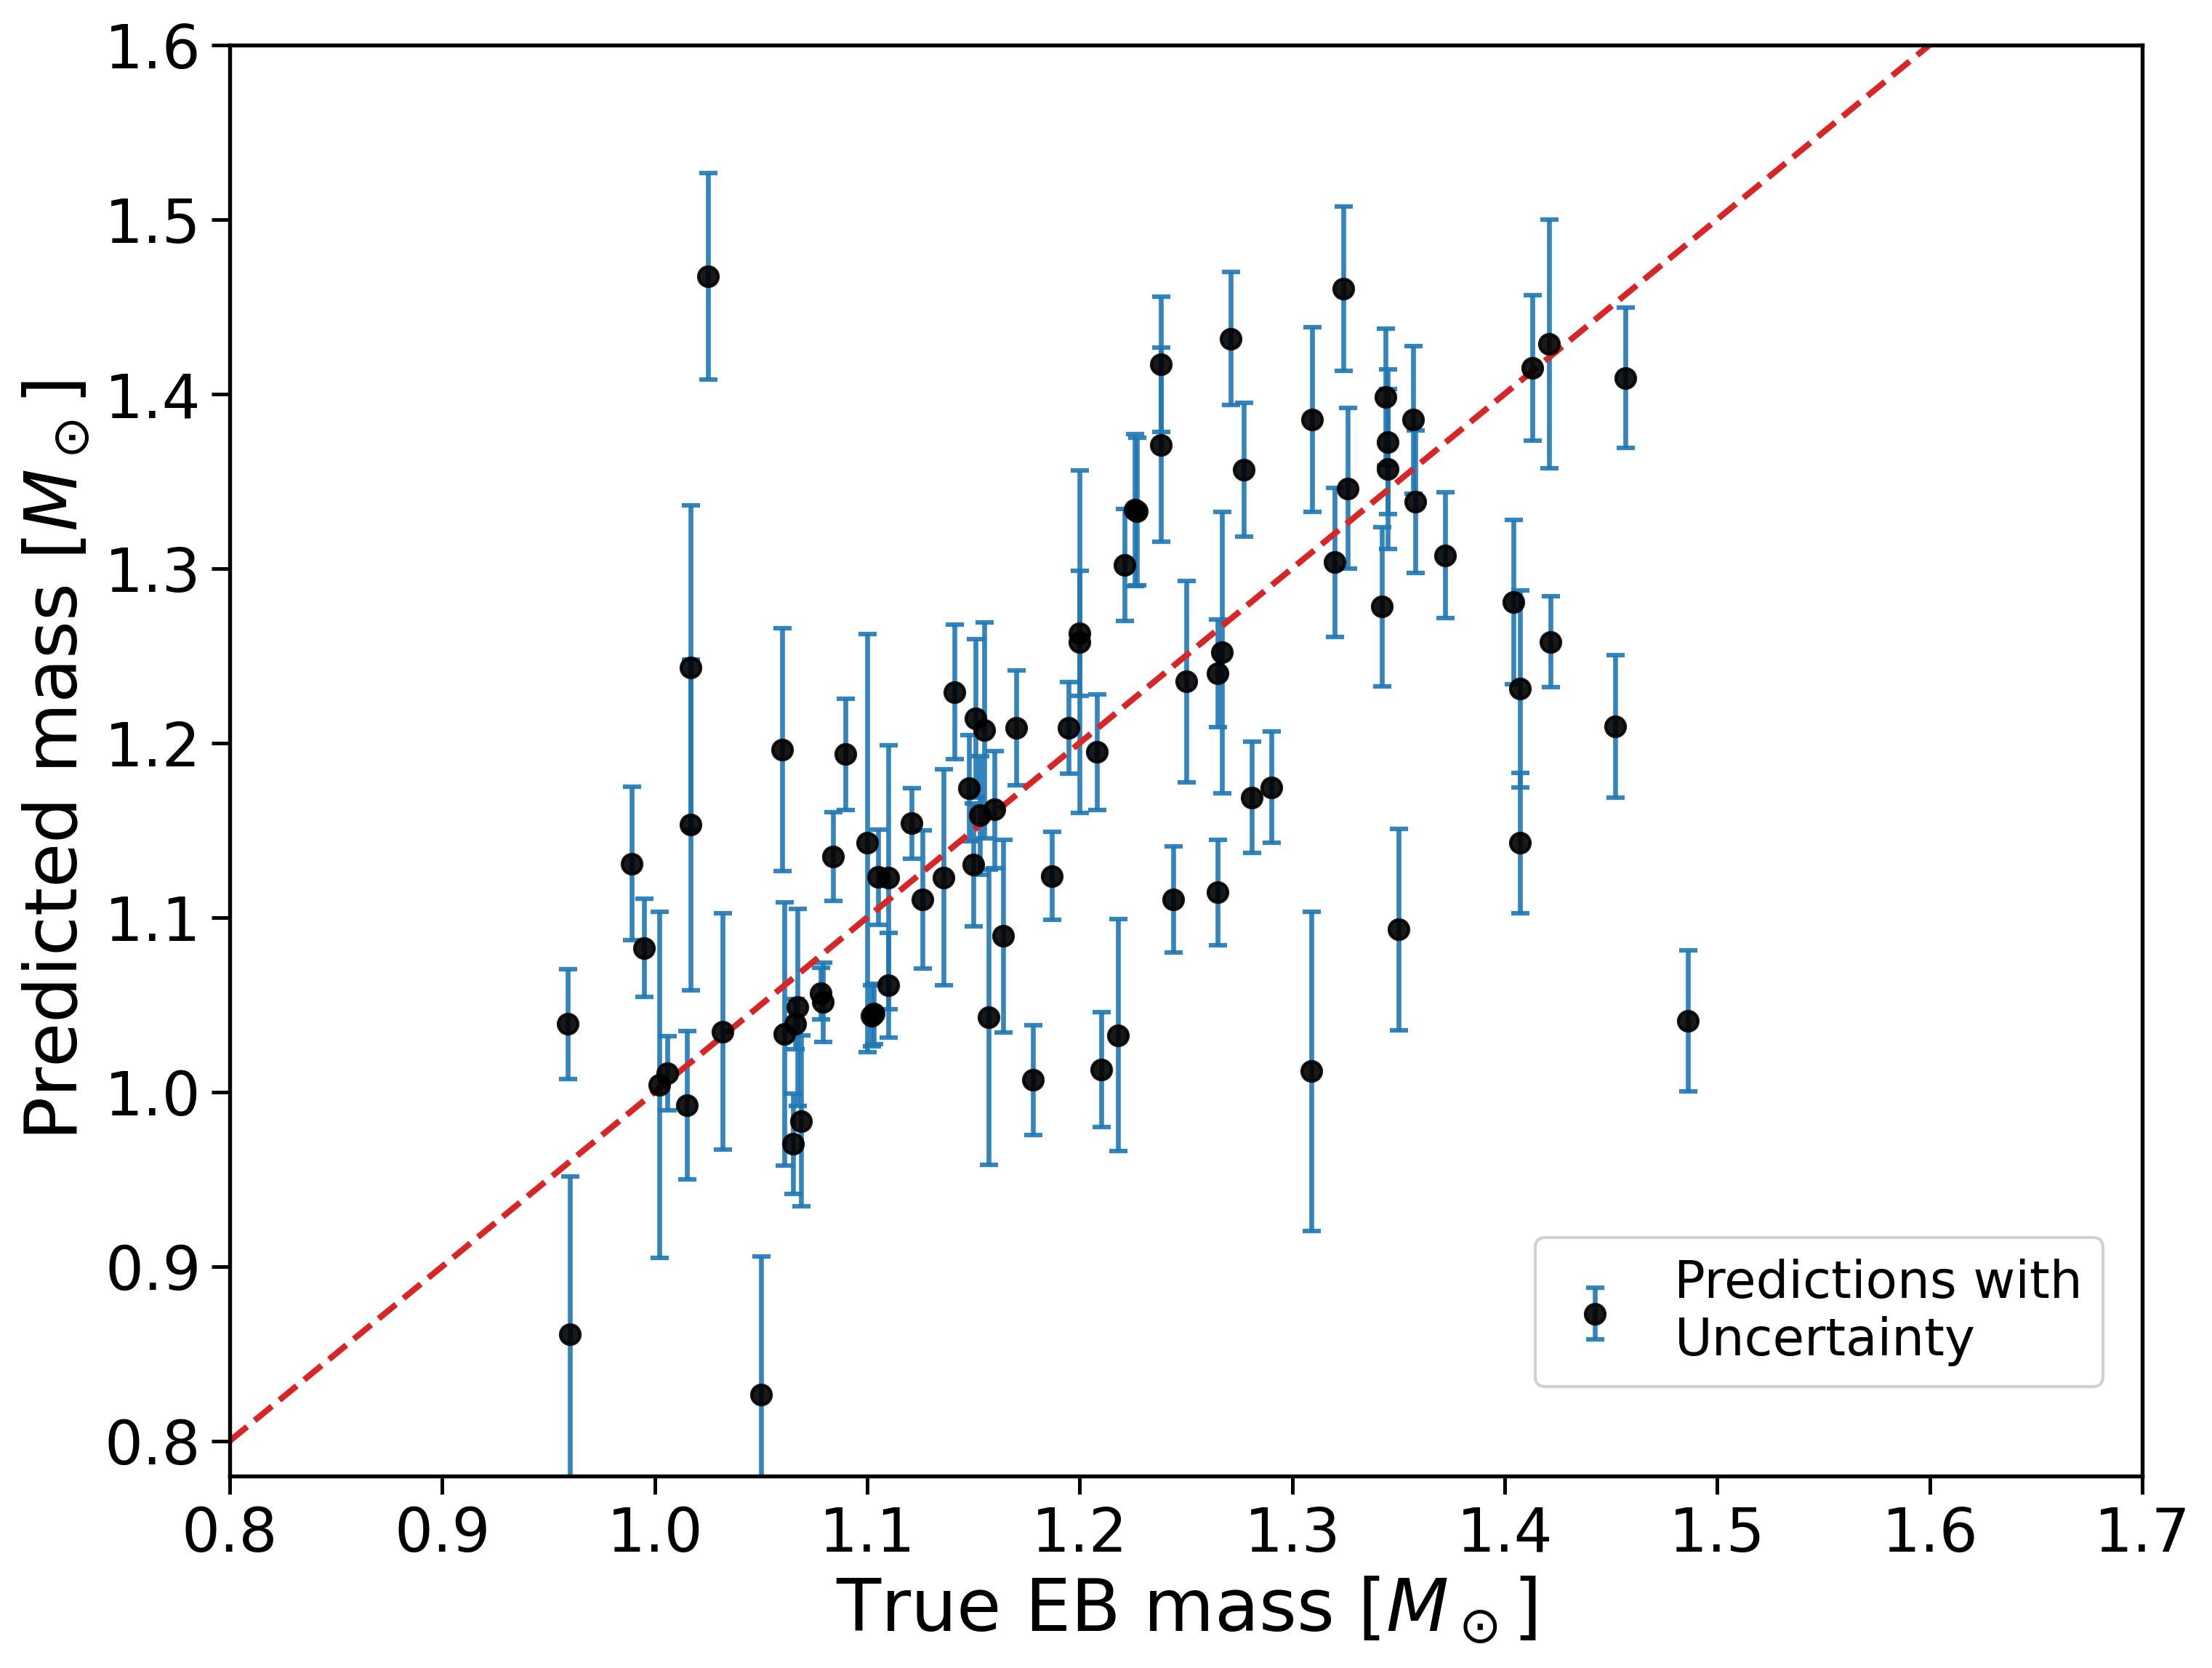
\includegraphics[width=\linewidth]{04_predicted_vs_true_EB_masses.png}
    \caption{Predicted masses.}
    \label{fig:dataset_D_mass_predictions}
\end{subfigure}
\hfill
\begin{subfigure}[t]{0.31\textwidth}
    \centering
    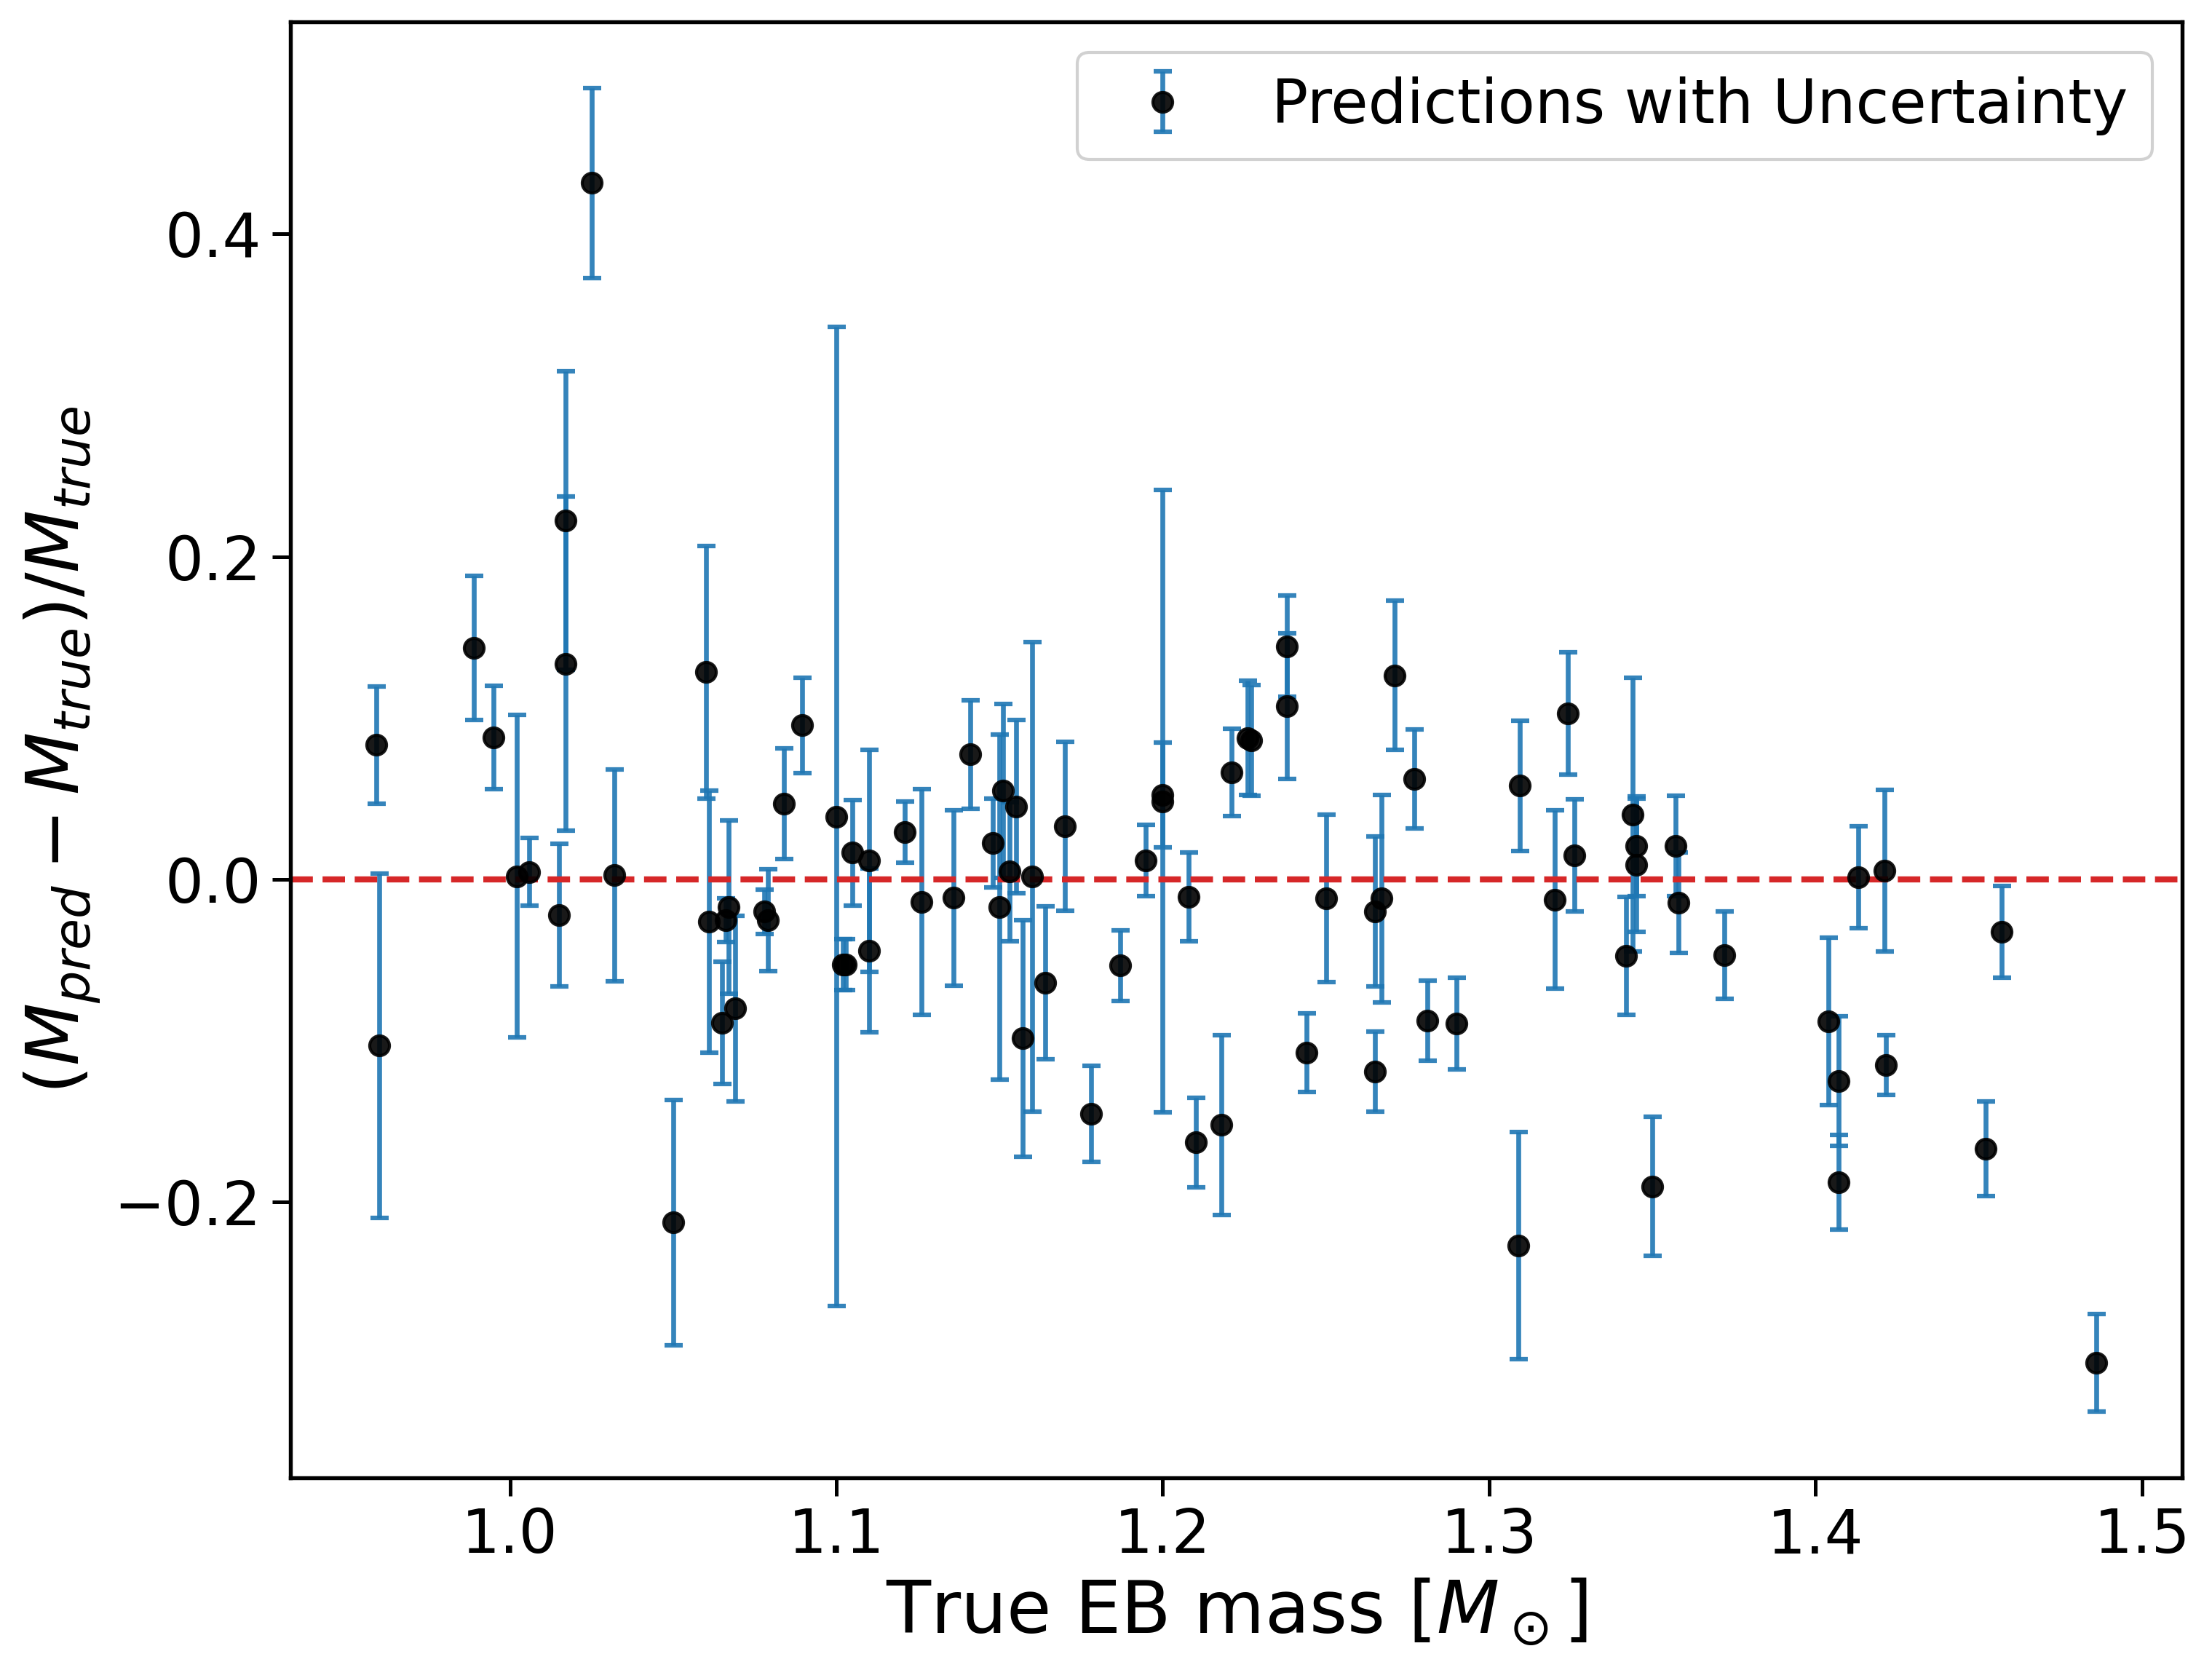
\includegraphics[width=\linewidth]{03_fractional_residual_vs_true_EB_mass.png}
    \caption{Fractional residuals.}
    \label{fig:dataset_D_mass_residuals}
\end{subfigure}
\hfill
\begin{subfigure}[t]{0.35\textwidth}
    \centering
    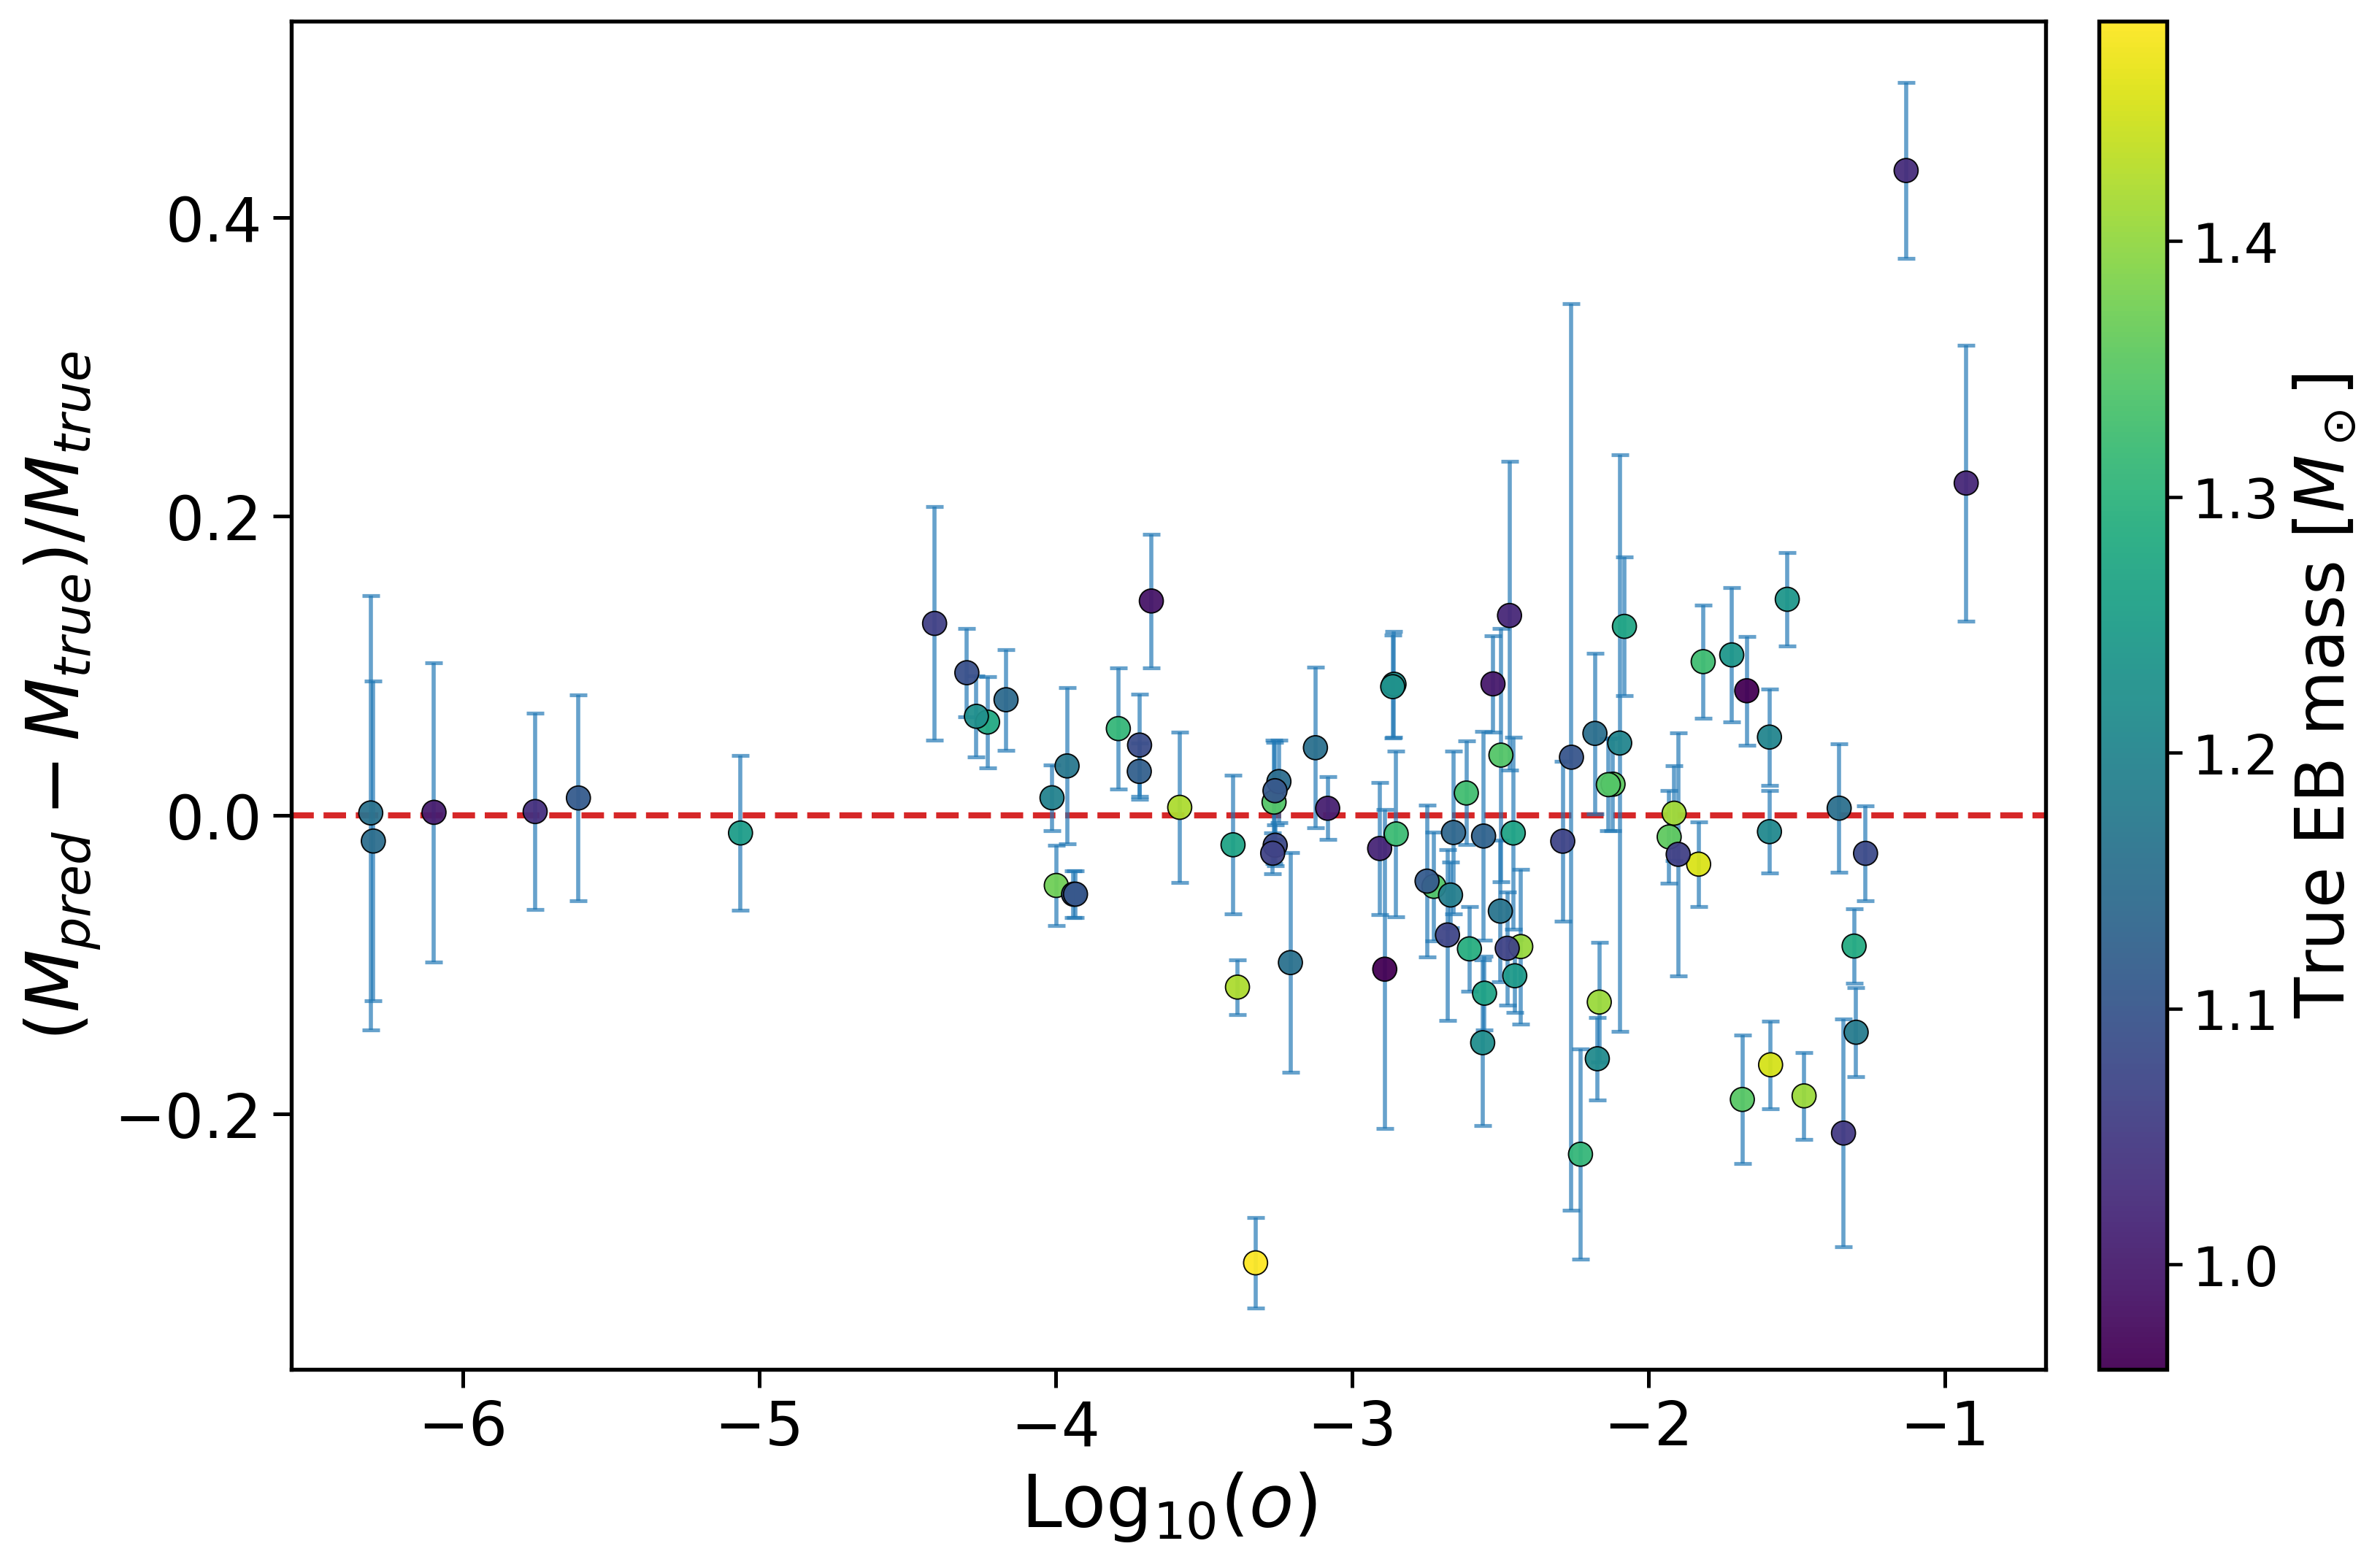
\includegraphics[width=\linewidth]{05_fractional_residual_vs_log10_oblateness_mass_colored.png}
    \caption{Fractional residuals, colour-coded by true mass.}
    \label{fig:dataset_D_o_residuals_mass_colored}
\end{subfigure}

\caption{Mass-prediction performance and mass dependence of the BHS residuals for the selected eclipsing-binary sample. The model uses $T_{\mathrm{eff}}$, $L$, $\log g$ and $[\mathrm{Fe}/\mathrm{H}]$ as input parameters. The left panel compares predicted and reference EB masses, the central panel shows the corresponding fractional residuals as a function of true mass, and the right panel shows the fractional residuals as a function of stellar oblateness $o$, colour-coded by true mass. Error bars show the propagated predictive uncertainty, and the dashed red line marks zero residual. The sample contains $n=85$ stars.}
\label{fig:dataset_D_mass}

\end{figure}

To test the dependence of the residuals on the different input parameters, a multivariable linear regression was performed on the eclipsing-binary residuals. Each feature, together with $o$ and $M$, was assigned a regression coefficient, $\beta$, quantifying its influence on the residual behaviour. Since the predictors were standardised, the coefficients can be directly compared.

The signed residuals are not significantly associated with oblateness, with $\beta_{\log o} = 0.002 \pm 0.005$, consistent with zero; $o$ does not introduce an overall positive or negative bias in the predictions. Instead, the signed residuals are mainly associated with the stellar parameters themselves. As already seen in Figure \ref{fig:dataset_D_mass}, mass affects the tendency towards overprediction or underprediction, with $\beta_M = -0.108 \pm 0.005$. Other relevant contributions are found for $T_{\mathrm{eff}}$, with $\beta_{T_{\mathrm{eff}}} = 0.077 \pm 0.007$, and for $[\mathrm{Fe}/\mathrm{H}]$, with $\beta_{[\mathrm{Fe}/\mathrm{H}]} = 0.048 \pm 0.002$.

The result changes when the absolute fractional residual is used as the response variable. In this case, $\log o$ is the only statistically significant predictor, with $\beta_{\log o} = 0.030 \pm 0.012$. Since the predictors are standardised, this means that a one-standard-deviation increase in $\log o$ is associated with an increase of about $3.0$ percentage points in $|\delta M|$. The remaining predictors are not significant in this regression.

The uncertainty calibration also suggests that eclipsing-binary stars are harder to predict than stars drawn from the training distribution, since an additional source of scatter appears when the asteroseismic-trained model is applied to eclipsing binaries. Only $30/85$ stars, or $35.3\%$, have their true mass within $1\sigma$ of the predictive interval.

\section{Conclusions} \label{sec:conclusions}

This work employed an uncertainty-aware stacking approach to obtain posterior predictive distributions for stellar masses using probabilistic machine-learning models. Three level-0 models, BART, HBNN and GP, were combined through Bayesian Hierarchical Stacking. The training set was constructed from high-quality reference catalogues based mainly on asteroseismology, detached eclipsing binaries and interferometry. The starting point was the 726 main-sequence-star catalogue of \citet{moya2018}, which was extended with recent literature sources published from 2018 onwards. After cleaning and cross-matching the samples, the final usable set consisted of 767 main-sequence stars, all of which had $M$, $T_{\mathrm{eff}}$, $L$, $[\mathrm{Fe}/\mathrm{H}]$ and $\rho$; 729 also had $\log g$, and 295 had $o$.

The first experiment tested the models on FGK-type stars, since this was the dominant stellar population in the final sample. Using a $20\%$ holdout set yielded mean absolute relative differences between predicted and reference masses which were all close to $5\%$, with the level-1 BHS model giving the best overall performance. HBNN and BART showed a systematic tendency to pull predictions towards approximately $1.25\,M_\odot$, where the training set is most densely populated. In contrast, GP showed no clear mass-dependent bias, although it produced a small number of outliers with unphysically large predictive uncertainties. The stacking model benefited from the complementary behaviour of the level-0 predictors and achieved an MRD of $0.20\%$, indicating negligible global bias.

The second experiment focused on a feature set with reduced model dependence, using $T_{\mathrm{eff}}$, $L$ and $[\mathrm{Fe}/\mathrm{H}]$ to estimate stellar masses. The qualitative behaviour of the three level-0 models and the stacking model remained similar to that found in the previous experiment, although the predictive precision worsened by approximately two percentage points. The models also showed a small overpredicting tendency, with the BHS model giving an MRD of $-1.36\%$. The predictions were then compared with evolutionary-grid estimates based on PARSEC \citep{bressan2012} and with linear-relation masses presented by \citet{moya2018}. The three approaches gave broadly compatible, but not identical results. A natural continuation of this analysis would be to combine all three approaches within a single stacking framework, so that the final estimate can benefit from the strengths of each method.

The third experiment showed that models trained on approximately single-star data can be transferred to eclipsing-binary components, but not without limitations. The oblateness parameter $o$ was introduced to quantify the degree of interaction between the two components, and the models were trained only on the assembled asteroseismic sample. The differences between the predicted and reference masses for eclipsing-binary stars were then analysed as a function of $o$. For the selected sample of 85 eclipsing-binary stars, oblateness did not introduce a significant signed mass bias, with $\beta_{\log o} = 0.002 \pm 0.005$. However, it did increase the absolute residuals, with $\beta_{\log o} = 0.030 \pm 0.012$, indicating a loss of precision rather than a systematic loss of accuracy. A practical transition point was found around $o \sim 0.01$, above which the residual scatter becomes large enough for the predictions to be considered less reliable.

\subsection*{Conclusiones}
\medskip
{\itshape
\noindent Este trabajo tom\'o un enfoque de stacking con tratamiento expl\'icito de incertidumbres para obtener distribuciones predictivas posteriores de masas estelares mediante modelos probabil\'isticos de machine learning. Tres modelos de nivel 0, BART, HBNN y GP, fueron combinados mediante Bayesian Hierarchical Stacking. El dataset de entrenamiento se construy\'o a partir de cat\'alogos de referencia de alta calidad, basados principalmente en astrosismolog\'ia, binarias eclipsantes e interferometr\'ia. El punto de partida fue el cat\'alogo de 726 estrellas de la secuencia principal recopilado por \citet{moya2018}, que se ampli\'o con fuentes bibliogr\'aficas recientes publicadas a partir de 2018. Tras la limpieza y el cruce de las muestras, el conjunto final utilizable qued\'o formado por 767 estrellas de la secuencia principal, todas ellas con $M$, $T_{\mathrm{eff}}$, $L$, $[\mathrm{Fe}/\mathrm{H}]$ y $\rho$; 729 tambi\'en ten\'ian $\log g$, y 295 ten\'ian $o$.

El primer experimento evalu\'o los modelos en estrellas de tipo FGK, dado que esta era la poblaci\'on estelar dominante en la muestra final. Utilizando un conjunto de prueba reservado del $20\%$, las diferencias relativas absolutas medias entre las masas predichas y las masas de referencia fueron todas pr\'oximas al $5\%$, con el modelo de stacking proporcionando el mejor rendimiento global. HBNN y BART mostraron una tendencia sistem\'atica a desplazar las predicciones hacia aproximadamente $1.25\,M_\odot$, donde el conjunto de entrenamiento se muestra m\'as densamente poblado. En cambio, GP no mostr\'o un sesgo claro dependiente de la masa, aunque produjo un reducido n\'umero de predicciones con incertidumbres f\'isicamente inveros\'imiles. El modelo de stacking se benefici\'o del comportamiento complementario de los predictores de nivel 0 y alcanz\'o un MRD de $0.20\%$, lo que indica un sesgo global despreciable.

El segundo experimento se centr\'o en un conjunto de variables de entrada con menor dependencia de modelos, utilizando $T_{\mathrm{eff}}$, $L$ y $[\mathrm{Fe}/\mathrm{H}]$. El comportamiento cualitativo de los tres modelos de nivel 0 y del modelo BHS se mantuvo similar al encontrado en el experimento anterior, aunque la precisi\'on predictiva empeor\'o en aproximadamente dos puntos porcentuales. Los modelos tambi\'en mostraron una leve tendencia a la sobrepredicci\'on, con el modelo BHS dando un MRD de $-1.36\%$. Las predicciones se compararon posteriormente con estimaciones basadas en modelos estelares de PARSEC \citep{bressan2012} y con predicciones mediante las relaciones lineales presentadas por \citet{moya2018}. Los tres enfoques dieron resultados compatibles, aunque no id\'enticos. La continuaci\'on natural de este an\'alisis ser\'ia combinar los tres enfoques dentro de un \'unico marco de stacking, de modo que la estimaci\'on final pueda beneficiarse de las fortalezas de cada m\'etodo.

El tercer experimento mostr\'o que los modelos entrenados con datos de estrellas individuales pueden transferirse a componentes de binarias eclipsantes, aunque no sin limitaciones. El par\'ametro de oblaticidad $o$ se introdujo para cuantificar el grado de interacci\'on entre las dos componentes, y los modelos se entrenaron \'unicamente con la muestra astrosismol\'ogica recopilada. Las diferencias entre las predicciones de masas y los valores de referencia para las estrellas binarias eclipsantes se analizaron entonces como funci\'on de $o$. Para la muestra seleccionada, 85 estrellas binarias eclipsantes, la oblaticidad no introdujo un sesgo signado de masa significativo, con $\beta_{\log o} = 0.002 \pm 0.005$. Sin embargo, s\'i aument\'o los residuos absolutos, con $\beta_{\log o} = 0.030 \pm 0.012$, lo que indica una p\'erdida de precisi\'on m\'as que una p\'erdida sistem\'atica de exactitud. Se encontr\'o un punto de transici\'on pr\'actico alrededor de $o \sim 0.01$, por encima del cual la dispersi\'on de los residuos se vuelve suficientemente grande como para considerar las predicciones menos fiables.
}


\bibliographystyle{aasjournal}
\bibliography{references}

\end{document}
\endinput}
\fi
\BayeStarMLMaybeInputMain

\documentclass[paper=a4, fontsize=12pt]{scrartcl}

\usepackage[british]{babel}
\usepackage[utf8]{inputenc}
\usepackage[T1]{fontenc}

% Mathematics
\usepackage{amsmath, amsfonts, amssymb, amsthm}
\usepackage{accents}
\usepackage{cancel}

% Units
\usepackage{siunitx}

% Figures and tables
\usepackage{graphicx}
\usepackage{epstopdf}
\usepackage{float}
\usepackage[labelfont=bf]{caption}
\usepackage{subcaption}
\captionsetup[table]{labelsep=period,singlelinecheck=false}

% Layout and formatting
\usepackage[a4paper,margin=22mm]{geometry}
\usepackage{sectsty}
\allsectionsfont{\normalfont\scshape\bfseries}
\sectionfont{\normalfont\Large\scshape\bfseries}
\setlength\parindent{15pt}

\usepackage{fancyhdr}
\pagestyle{fancy}
\fancyhead{}
\fancyfoot[L]{}
\fancyfoot[C]{}
\fancyfoot[R]{\thepage}
\renewcommand{\headrulewidth}{0pt}
\renewcommand{\footrulewidth}{0pt}
\setlength{\headheight}{13.6pt}

\usepackage{setspace}
\setstretch{1.15}

\newcommand{\horrule}[1]{\rule{\linewidth}{#1}}

% Other packages
\usepackage{lipsum}
\usepackage{xcolor}
\usepackage{makeidx}
\usepackage{fancybox}
\usepackage{tikz}
\usepackage[most]{tcolorbox}
\usepackage{multicol}

% Background
\usepackage[pages=some]{background}
\backgroundsetup{
 scale=1,
 color=black,
 opacity=1,
 angle=0,
 contents={
 
\includegraphics[height=\paperheight]{Figuras/Fondo.pdf}
 }
}
\usepackage{wallpaper}

% Bibliography
\usepackage[round,authoryear]{natbib}
\setlength{\bibsep}{0pt plus 0.2ex}
\providecommand{\bibfont}{}
\renewcommand{\bibfont}{\normalfont\normalsize\setstretch{1.0}}

% Hyperref should be near the end
\usepackage[hidelinks=true, hyperfootnotes=false]{hyperref}
